% !TeX program = pdflatex -> bibtex -> pdflatex * 2
% Documento unificado. Compilar desde esta carpeta: pdflatex, biber propuesta, pdflatex, pdflatex.
% Si las bibliografias por curso muestran entradas de otro curso, borre propuesta.bbl (y propuesta.bcf) y vuelva a compilar todo el ciclo: un .bbl desactualizado respecto al .bcf desordena las refsections.
\documentclass[11pt]{report}

\input{propuesta-preamble}

\begin{document}

\begin{titlepage}
\thispagestyle{empty}
\begin{tikzpicture}[remember picture, overlay]
  % Fondo
  \fill[Azul-UCR] (current page.south west) rectangle (current page.north east);

  % Franja lateral
  \fill[Celeste-UCR] (current page.south west) rectangle ([xshift=0.85cm]current page.north west);
  \fill[Amarillo-UCR] ([xshift=0.85cm]current page.south west) rectangle ([xshift=1.00cm]current page.north west);

  % Formas decorativas
  \fill[Celeste-UCR, opacity=0.16]
    ([xshift=-1.6cm, yshift=-1.4cm]current page.north east) circle (5.4cm);
  \fill[Verde-UCR, opacity=0.14]
    ([xshift=-0.4cm, yshift=-9.2cm]current page.north east) circle (3.6cm);
  \fill[Amarillo-UCR, opacity=0.10]
    ([xshift=1.8cm, yshift=3.4cm]current page.south east) circle (4.2cm);

  % Malla: nodos y aristas (metáfora del plan de estudios)
  \begin{scope}[shift={([xshift=-7.55cm, yshift=-12.6cm]current page.north east)}]
    \foreach \x in {0,1,2,3} {
      \foreach \y in {0,1,2,3,4} {
        \draw[white, opacity=0.18, line width=0.6pt]
          (\x*1.42, -\y*1.28) -- (\x*1.42, -\y*1.28-1.28);
      }
    }
    \foreach \x in {0,1,2} {
      \foreach \y in {0,1,2,3,4,5} {
        \draw[white, opacity=0.18, line width=0.6pt]
          (\x*1.42, -\y*1.28) -- (\x*1.42+1.42, -\y*1.28);
      }
    }
    \foreach \x in {0,1,2,3} {
      \foreach \y in {0,1,2,3,4,5} {
        \fill[white, opacity=0.22] (\x*1.42, -\y*1.28) circle (0.19);
      }
    }
    \draw[Celeste-UCR, line width=1.55pt]
      (0,0) -- (1.42,-1.28) -- (2.84,-1.28) -- (2.84,-3.84) -- (4.26,-5.12);
    \fill[Amarillo-UCR] (0,0) circle (0.30);
    \fill[Celeste-UCR] (1.42,-1.28) circle (0.24);
    \fill[Celeste-UCR] (2.84,-1.28) circle (0.24);
    \fill[Celeste-UCR] (2.84,-3.84) circle (0.24);
    \fill[Verde-UCR] (4.26,-5.12) circle (0.30);
  \end{scope}

  % Encabezado institucional
  \node[anchor=north west]
    at ([xshift=2.15cm, yshift=-1.45cm]current page.north west) {
      
\includegraphics[height=1.45cm]{assets/logos/firma-ucr-blanco.png}
    };

  % Texto principal
  \node[anchor=north west, inner sep=0pt]
    at ([xshift=2.15cm, yshift=-4.15cm]current page.north west) {
      \begin{minipage}{12.4cm}
        \color{white}\raggedright
        {\color{Celeste-UCR}\fontsize{12}{14}\selectfont\bfseries PROPUESTA CURRICULAR\par}
        \vspace{10pt}
        {\fontsize{36}{40}\selectfont\bfseries
        Propuestas de\\
        modificación\\
        curricular\par}
        \vspace{12pt}
        {\color{Amarillo-UCR}\rule{3.15cm}{3.2pt}\par}
        \vspace{14pt}
        {\fontsize{16}{20}\selectfont
        Bachillerato y Licenciatura\\
        en Matemática\par}
      \end{minipage}
    };

  % Pie
  \node[anchor=south west, inner sep=0pt]
    at ([xshift=2.15cm, yshift=2.35cm]current page.south west) {
      \begin{minipage}{10cm}
        \color{white}\raggedright
        
\includegraphics[height=1.7cm]{assets/logos/logo-mate.png}\\[12pt]
        {\fontsize{12}{15}\selectfont Comisión de Malla Curricular\par}
        {\color{Celeste-UCR}\fontsize{12}{15}\selectfont \the\year\par}
      \end{minipage}
    };
\end{tikzpicture}
\end{titlepage}

\tableofcontents


\clearpage

\chapter{Introducción}
\chapter{Introducción}


En los últimos años se han realizado esfuerzos para transformar las carreras que pertenecen a la Escuela de Matemática de la Universidad de Costa Rica. Un paso iniciial se dio con la creación de la carrera de Educación Matemática, que, en el año 2017, abrió las puertas e integró una primera generación de estudiantes. Un año después, se consideró la necesidad de reestructurar las carreras de Matemática y Ciencias Actuariales, para lo cual se inició un proceso de manera conjunta. En el año 2019 se hizo la separación de los procesos con el fin de que se pudieran desarrollar los apartados necesarios para la construcción del perfil de cada carrera por aparte. Este documento constituye una nueva propuesta para el plan de estudios de la carrera de Matemática.

El proceso ha sido largo. En el periodo 2018-2020, se propuso un camino que estuvo mediado por una subcomisión de la Comisión de Docencia de la Escuela de Matemática, en el que se incorporaron las apreciaciones de docentes y estudiantes, así como una revisión de las prácticas llevadas a cabo en las últimas décadas. Esto permitió llegar a establecer el perfil de salida de lo que consideramos será un matemático del siglo XXI \footfullcite{Comision20}. Tal documento se encuentra incluido en el presente trabajo.

Como parte de las incorporaciones de cambio en la reestructuración de la malla curricular, a la luz del trabajo en los marcos referenciales y el establecimiento del perfil de salida, se determinaron cinco áreas curriculares que orientan el trabajo propuesto para alcanzar los propósitos establecidos. Dichas áreas son: habilidades operacionales, pensamiento abstracto, formalismo, pensamiento algorítmico y habilidades investigativas. Este documento no ahonda en tales áreas, pero constituye un fundamento previo para justificar la presencia de estas en la selección y organización de los contenidos, así como la gestión curricular. 

El proceso llevó a la conclusión de la importancia de incorporar dos énfasis en la carrera: Una ruta más teórica o pura que sigue un enfoque más orientado a formar investigadores en áreas puras de la matemática y otro camino más aplicado, dedicado también a formar investigadores pero abierto también a la formación de profesionales que puedan desenvolverse en otros entornos institucionales no académicos o empresariales.

%En este documento se presentan cuatro apartados. Se inicia con la metodología que describe el proceso de los dos años de trabajo para la elaboración del perfil de salida. Se amplía con un contexto teórico y reflexivo de los marcos referenciales que orientan la toma de decisiones para la presentación final de la reestructuración, unida con el aporte de los docentes que participaron en las diferentes actividades donde se recopilaron datos. En los dos últimos apartados se incluyen la declaración de propósitos y el perfil de salida de la carrera de Matemática, aporte que no había sido contemplado anteriormente desde la creación de la carrera, por lo que se considera una transformación en la forma de concebir esta disciplina en el plan de formación. 

Este documento se estructura de acuerdo con los lineamientos establecidos en \cite{Bolanos15} y \cite{CEA24}. 

\section{Metodología}

En esta sección se mencionan algunos aspectos de la metodología que se usó para la conceptualización de la propuesta curricular y la elaboración de este documento.

%se especifican tres aspectos: la conformación del equipo encargado de este documento, los mecanismos que se llevaron a cabo para la obtención de la información, y, por último, una breve noción de lo que representó diseñar este proceso de construcción del perfil de salida, posterior a la elaboración de los marcos referenciales que son pilares fundamentales para esta y otras etapas que se requieren para la reestructuración de la carrera de Matemática. 

\subsection{El equipo de trabajo}

El inicio del perfil de salida viene por mandato de la Vicerrectoría de Docencia (cf.VD-3575-2017) y según designación del Dr. William Ugalde Gómez, director de la Escuela de Matemática, se asignó la responsabilidad. Posterior a una reunión en enero del 2018, junto con las asesoras del CEA, se comprendió la complejidad de esta labor y se conformó un equipo junto con otros tres integrantes, de donde surgió la subcomisión de la Comisión de Docencia que se encargaría de la elaboración del perfil de salida de la carrera. 

El proceso requería una revisión profunda en aspectos epistemológicos y pedagógicos, así como la importancia de dedicar espacios para interactuar con los miembros de la Escuela de Matemática; se acordó en febrero del 2018 la inserción de un estudiante avanzado de la carrera de Enseñanza de la Matemática, quien, posteriormente, se incorporó como miembro de la subcomisión. En agosto del 2019, y durante los siguientes seis meses, se incorporó a otro estudiante con el mismo perfil, que brindó un importante apoyo en la realización de actividades para la obtención de insumos teóricos. Finalmente, la subcomisión concluyó sus labores con tres miembros en julio del 2020 en el contexto del COVID-19, lo cual indujo una participación vía remota y una forma diferente de articular la responsabilidad de concluir el presente documento. 

Los miembros de la subcomisión se encargaron de plantear las estrategias para construir cada uno de los marcos referenciales, orientados por los documentos suministrados y la guía brindada por las asesoras asignadas por el CEA. Además, ellos organizaron las actividades de consulta, realizaron discusión y análisis de la información, y posteriormente, la redacción de cada uno de los apartados. Finalmente, en aquellos aportes que se juzgó necesario, se compartía el trabajo realizado con otros miembros de la Escuela de Matemática, quienes, en muchas ocasiones, dieron importantes contribuciones y una oportuna intervención para asegurar que el trabajo realizado presentaba las características adecuadas. 

A partir del año 20... se cambió la conformación...

Con la llegada del Dr. Pedro Méndez a la dirección de la Escuela de Matemáticas en el año 2025 de nuevo hubo cambios en la conformación ...

\subsection{Las actividades realizadas}

Como parte del proceso se llevaron a cabo numerosas actividades de diversos tipos. Procedemos a describir brevemente las principales.

\subsubsection{Reuniones de la comisión}

...

% \subsection{Espacios de consulta, técnicas de recopilación y análisis de la información}

% Como se observa en la siguiente imagen, se consideraron cinco modalidades para incorporar información pertinente a la redacción del presente documento, cuyo proceso de construcción se justifica según la necesidad de requerir la intervención de otros actores, además de los miembros de la subcomisión. Dicho proceso se prolongó durante dos años y su razón de ser se esboza a continuación. 

\subsubsection{Entrevista}

En un proceso de reflexión inicial para determinar qué es la matemática, se propusieron diferentes áreas de la Matemática, las cuales están bien representadas por miembros de la Escuela de Matemática de la Universidad de Costa Rica; a estas áreas se les llamó identidades. Lo anterior obedece a la complejidad que conlleva establecer este concepto y lo que requiere la construcción de un instrumento denominado V heurística, con el fin de identificar lo teórico y metodológico de cada identidad. Se eligió a uno o dos docentes para que fuesen entrevistados, según la identidad correspondiente. Inicialmente, se determinaron las siguientes identidades: lógica, probabilidad, estadística, geometría, álgebra, análisis, análisis numérico, teoría de números, topología, modelización matemática, análisis funcional y ecuaciones diferenciales.

Con la entrevista se buscaba determinar en qué consiste cada una de las identidades por medio de seis preguntas, cuyos resultados están presentes en el Anexo 1. El proceso de consulta se llevó a cabo entre abril y julio del 2018.

\subsubsection{Grupos focales}

La construcción de cada una de las V heurísticas, según la identidad matemática correspondiente, logró alcanzar el fin esperado excepto en el caso de álgebra, análisis y geometría. Esto puede deberse a que estas tres áreas son las de mayor predominio en la Matemática. Se acordó, por tanto, establecer tres espacios para realizar grupos focales, donde se reunían de cuatro a seis especialistas según la identidad. Los grupos focales procuraban dar respuesta a las preguntas que se diseñaron para la entrevista, con la posibilidad adicional de escuchar otros puntos de vista.

Los tres grupos focales fueron grabados y, después de la transcripción y posterior análisis, se logró construir las tres V heurísticas faltantes. Los grupos focales se aplicaron en el mes de octubre del 2018. 

\subsubsection{Análisis estructurales de la actividad}

Según cada identidad matemática, se procuró un proceso de mayor análisis para profundizar en cada objeto matemático y en el establecimiento de las acciones que lleva a cabo el especialista de esa área. La construcción del análisis estructural de la actividad permitió visualizar la conexión entre el marco socio profesional y el pedagógico, así como la identificación de gran parte de los conocimientos y habilidades descritos en el perfil de salida propuesto. 

La subcomisión diseñó cuatro de estos análisis estructurales; pero, conforme se avanzaba, iban surgiendo más dudas que respuestas de lo que se procuraba alcanzar. Como consecuencia de
muchos momentos de discusión, al considerar el proceso que ya se había desarrollado, tanto en el marco socio profesional como epistemológico, se concluyó que la estadística dejaba de formar parte de las identidades; ya que, esta área está más relacionada con la carrera de ciencias actuariales. Además, durante el desarrollo del análisis estructural del área del análisis matemático, se consideró también que la identidad de análisis funcional se incorporaba a la identidad análisis. En total se llevaron a cabo diez intervenciones para la construcción de los análisis estructurales de la actividad, ya que se acordó la convocatoria de especialistas, según cada área, para diseñar cada uno de estos, con la presencia de al menos un integrante de la subcomisión. Este proceso se extendió alrededor de 8 meses (con la realización de 20 reuniones desde los intentos iniciales, pasando por la incorporación de los especialistas y el análisis de los resultados obtenidos), durante los cuales se alterno con otras actividades del proceso, como lo fue el planeamiento y ejecución de talleres. 


\subsubsection{Talleres}

Como la elaboración de los marcos referenciales es un apartado para construirse según las creencias, vivencias y expectativas de los que conforman la Escuela de Matemática, en cuanto a la carrera de Matemática corresponde, se destinaron tres momentos para la realización de talleres. Estos contaron con la participación de más de veinte personas en cada uno. Para la escogencia de los participantes, se buscó mantener el mejor equilibrio posible en cuanto a género, edad, años de servicio y área de especialización. Además, se solicitó la presencia de algunos estudiantes avanzados de la carrera. 

En el primer taller se extrajo información para iniciar la experiencia de la construcción del marco pedagógico. Se recabó información asociada a las formas en las cuales los participantes enseñan o han aprendido Matemática, las estrategias que aplican actualmente y su visión sobre la futura malla curricular que deberá resultar de este proceso de reestructuración de la carrera. En el segundo taller se trabajó en la obtención de información para el marco epistemológico, para ir construyendo la noción de qué es la matemática, no a partir de lo que dicen las fuentes o especialistas internacionales, sino de la concepción interna de los participantes.

Por último, en el tercer taller, hubo espacio para que los docentes dieran aportes de la posible construcción de una malla curricular, que considerara las áreas curriculares que fueron especificadas previamente. Para esto, se les entregó un material que explicaba las diferentes formas de acceder al aprendizaje según el tipo de curso que se propusiera. En el Anexo 2 se muestra el documento que las asesoras del CEA facilitaron, pero cuyo aporte tendrá mayor incidencia en la propuesta de la reestructuración. Aun así, esto brindó también insumos para la construcción del perfil de salida, e inclusive, para la declaración de propósitos. 

\subsubsection{Consultas, principalmente por correo electrónico}

La subcomisión se reunía con frecuencia para compartir cada uno de los avances e ir estableciendo acuerdos sobre cada aporte generado, en el proceso de construcción del documento. En el transcurso de la experiencia, se vislumbra, por un lado, la oportunidad de enriquecer diferentes apartados al compartir el producto teórico elaborado con otros colegas; y, por el otro, la urgencia de solicitar información ante diferentes escenarios, cuando los propios miembros de la subcomisión consideraban que no tenían la respuesta o alguna forma de dar inicio con esa asignación. La consulta por correo electrónico a diferentes miembros de la Escuela de Matemática fue muy valiosa; se describe, a continuación, en cuáles apartados fue que se contribuyó directamente para la finalización de este documento: principales hitos de la historia de la matemática, historia del desarrollo de la matemática en Costa Rica, prácticas emergentes, decadentes y dominantes, cuadros finales de los análisis estructurales de la actividad, importancia de las identidades matemáticas determinadas en el marco epistemológico, la finalidad de la matemática, perfil de salida, entre otros.


\chapter{Antecedentes y justificación}
\chapter{Antecedentes y justificación}

\section{Antecedentes de la carrera en la UCR}

La formación universitaria en matemática en Costa Rica tiene sus raíces en la Escuela de Ciencias de la Universidad de Costa Rica, creada en 1940, donde la disciplina atendía principalmente las necesidades de otras carreras y la formación de profesores para enseñanza media. En 1957, con la Reforma Universitaria de Rodrigo Facio, se integró el Departamento de Física y Matemáticas, antecedente directo de la carrera profesional en Matemática. En 1971 se creó el Departamento de Matemáticas y, producto del Tercer Congreso Universitario (1972--1973), en 1974 el departamento se convirtió en Escuela de Matemática, con autonomía para impartir y administrar su propia carrera.

Desde entonces, la Escuela ha ofrecido Bachillerato y Licenciatura en Matemática en la Sede Rodrigo Facio (Campus Universitario). Entre los principales hitos curriculares e institucionales se destacan: la Licenciatura en Matemática (1967--1972), el plan con énfasis purista vigente entre 1973 y 1991 (124 créditos de bachillerato y 30 de licenciatura), las reformas de 1992 (cursos optativos interdisciplinarios y ajustes al primer año), el Programa de Maestría en Matemáticas (desde 1980), la creación de los centros CIMM y CIMPA en la década de 1990, y la consolidación de la investigación y la divulgación mediante publicaciones como la \emph{Revista de Matemática: Teoría y Aplicaciones}.

En 2017 se abrió la carrera de Educación Matemática. Un año después inició, de manera conjunta con Ciencias Actuariales, un proceso de reestructuración curricular que en 2019 se separó por carrera. Entre 2018 y 2020, una subcomisión de la Comisión de Docencia de la Escuela---con apoyo del Centro de Enseñanza y Aprendizaje (CEA) y mandato de la Vicerrectoría de Docencia---elaboró el perfil de salida y los marcos referenciales que fundamentan la presente propuesta. Ese trabajo incorporó entrevistas, grupos focales, análisis estructurales de la actividad, talleres con docentes y estudiantes, y consultas a la comunidad académica.

Actualmente la Escuela de Matemática cuenta con 128 profesores (41 con grado de doctor), organizados en tres departamentos: Matemática Pura y Ciencias Actuariales, Educación Matemática, y Matemática Aplicada. El Bachillerato y Licenciatura en Matemática se imparten desde el Departamento de Matemática Pura y Ciencias Actuariales. La propuesta curricular que se presenta responde a la necesidad de actualizar un plan cuyo último rediseño integral data de hace más de tres décadas, en un contexto marcado por la digitalización, la interdisciplinariedad y nuevas demandas del mercado laboral y de la investigación.


\section{Justificación socioprofesional}

La Matemática ocupa un lugar central en el desarrollo científico, tecnológico y social contemporáneo. La digitalización de la información, el avance de la inteligencia artificial, el manejo de datos a gran escala y la modelación de fenómenos complejos han ampliado tanto el objeto de estudio de la disciplina como los ámbitos en que el matemático puede incidir. La UNESCO proclamó el 14 de marzo como Día Internacional de las Matemáticas (2019) y subraya su papel en el logro de los Objetivos de Desarrollo Sostenible, en la formación de capacidades para enfrentar desafíos como el cambio climático, la salud pública y la innovación tecnológica.

En este marco, la carrera de Matemática de la UCR debe formar profesionales competentes para la academia, el sector productivo y la interacción con otras disciplinas. La propuesta de plan de estudios articula cinco áreas curriculares---habilidades operacionales, pensamiento abstracto, formalismo, pensamiento algorítmico y habilidades investigativas---y nuevos espacios formativos (modelación matemática, seminario, comunicación en las ciencias, énfasis en matemática pura y aplicada) que responden a las demandas actuales y futuras del ejercicio profesional.


\subsection{Caracterización profesional}

\subsubsection{Radiografía laboral}

A nivel internacional, las ocupaciones vinculadas con la matemática muestran una demanda creciente. La Oficina de Trabajo Estadístico de Estados Unidos proyectó un aumento del 28\,\% en empleos matemáticos entre 2016 y 2026, superior al promedio de otras ocupaciones, impulsado por el \emph{big data} y la analítica. En rankings como los de CareerCast (2016), figuras como analista de datos, estadístico, matemático y actuario ocupan posiciones destacadas entre las mejores profesiones; carreras con alto contenido matemático (ciencias de la computación, ingeniería, economía, meteorología, entre otras) también se ubican en los primeros lugares.

En Costa Rica, el matemático encuentra oportunidades en instituciones de educación superior e investigación, centros como el CIMM y el CIMPA, organismos públicos y privados que requieren modelación, análisis cuantitativo y apoyo a la toma de decisiones, así como en sectores como finanzas, banca, economía, tecnología y servicios basados en datos. La separación de funciones actuariales hacia la carrera de Ciencias Actuariales y la especialización docente en Educación Matemática redefinen el espacio ocupacional del matemático, orientándolo hacia la investigación, la docencia universitaria, la modelación, el análisis de datos y el trabajo interdisciplinario.

La formación en Matemática desarrolla capacidades analíticas, rigor argumentativo y resolución de problemas que son valoradas transversalmente por empleadores, conforme a evidencia en neurociencia cognitiva y a la propia naturaleza de la disciplina como lenguaje universal de las ciencias.


\subsubsection{Situación de la población graduada}

En el marco del proceso de reestructuración 2018--2020, la Escuela de Matemática recopiló información sobre las prácticas profesionales vigentes mediante entrevistas a especialistas, análisis estructurales de la actividad por identidad matemática, talleres con docentes y estudiantes avanzados, y consultas a la comunidad académica. Esos insumos permitieron caracterizar los escenarios de inserción y las funciones que desempeñan los matemáticos formados en la UCR.

De manera consistente con ese análisis, la población graduada se inserta principalmente en la docencia e investigación universitaria, en la modelación matemática de fenómenos de otras disciplinas y, de manera creciente, en el sector productivo (finanzas, banca, análisis de datos, consultoría cuantitativa). La dificultad para acceder a empleos directamente vinculados con la carrera varía según el ámbito: persiste demanda en academia e investigación, mientras que la enseñanza en secundaria y las labores actuariales han quedado en mayor medida a cargo de profesionales de Educación Matemática y Ciencias Actuariales, respectivamente.

La valoración de la formación recibida---especialmente respecto del perfil de egreso---constituyó insumo central para la elaboración del perfil de salida propuesto, que por primera vez explicita las competencias del matemático del siglo XXI. En la etapa de formalización curricular, la unidad académica complementará este apartado con el seguimiento institucional a las últimas cohortes graduadas, conforme a los lineamientos del Observatorio Laboral de Profesiones (OLAP) y otras fuentes nacionales.


\subsubsection{Campos de inserción laboral}

Los principales campos de inserción identificados para el matemático formado en la UCR son:

\begin{itemize}
  \item \textbf{Investigación académica} (teórica y aplicada), en universidades, centros de investigación y redes científicas nacionales e internacionales.
  \item \textbf{Docencia universitaria}, en programas de pregrado y posgrado en matemática y disciplinas afines.
  \item \textbf{Modelación matemática}, en ingeniería, física, biología, epidemiología, ciencias ambientales y otras áreas que requieren traducir problemas reales al lenguaje matemático.
  \item \textbf{Análisis de datos y ciencia de datos}, en empresas, instituciones financieras, organismos públicos y proyectos de investigación interdisciplinaria.
  \item \textbf{Sector productivo e industrial}, en roles de consultoría cuantitativa, optimización, criptografía, simulación y apoyo a la innovación tecnológica.
  \item \textbf{Trabajo interdisciplinario}, como puente entre equipos de distintas disciplinas en proyectos científicos, tecnológicos o de política pública.
\end{itemize}


\subsubsection{Funciones o tareas profesionales}

Para cada campo de inserción, el matemático desempeña funciones que, sintetizadas a partir del análisis estructural de la actividad realizado en la Escuela, incluyen:

\begin{itemize}
  \item Estudiar, clasificar y relacionar estructuras matemáticas (algebraicas, geométricas, analíticas, topológicas, probabilísticas, etc.) para comprender y resolver problemas.
  \item Formular conjeturas, demostrar resultados y contribuir a la creación de conocimiento matemático original.
  \item Traducir problemas de la vida real o de otras disciplinas al lenguaje matemático, seleccionar herramientas adecuadas y comunicar resultados en lenguaje interdisciplinario.
  \item Modelar fenómenos naturales, sociales o tecnológicos mediante ecuaciones, simulaciones y métodos numéricos o estocásticos.
  \item Analizar e interpretar datos, identificar patrones y apoyar la toma de decisiones basada en evidencia.
  \item Enseñar matemática en el ámbito universitario, diseñar experiencias de aprendizaje y orientar procesos de formación e investigación.
  \item Divulgar la producción científica mediante artículos, informes, presentaciones y participación en congresos y seminarios.
\end{itemize}

Estas funciones orientan la definición del perfil de egreso y la selección de contenidos, competencias y tipos de curso de la malla propuesta.


\subsection{Contribución al desarrollo del país}

La Matemática contribuye al proyecto humanista de la Universidad de Costa Rica al formar profesionales capaces de producir y aplicar conocimiento riguroso al servicio de la sociedad. Las matemáticas son herramienta para el desarrollo sostenible: modelan cambios ambientales y epidemiológicos, optimizan recursos en salud pública y transporte, sustentan la criptografía y las comunicaciones seguras, y apoyan la inteligencia artificial y el aprendizaje automático con aplicaciones en medicina, agricultura, energía y gobernanza.

En el plano nacional, la Escuela de Matemática ha sido pionera en la introducción de las matemáticas modernas en la enseñanza secundaria (Conferencia Interamericana de Educación Matemática, Bogotá, 1961) y mantiene un rol activo en la producción de conocimiento mediante el CIMM, el CIMPA y la Maestría en Matemáticas. La investigación y divulgación matemática enriquecen la cultura científica del país, fortalecen la formación de cuadros docentes e investigadores y generan capacidades para la innovación en sectores estratégicos de la economía costarricense.

La propuesta curricular responde además a compromisos institucionales y a marcos internacionales como los Objetivos de Desarrollo Sostenible y las prioridades de la UNESCO en ciencias básicas, educación matemática e igualdad de género. Al incorporar énfasis en matemática pura y aplicada, modelación, computación y comunicación científica, el plan busca que los graduados contribuyan a la calidad de vida de las personas, al crecimiento del capital humano avanzado y a la generación de oportunidades laborales en ámbitos emergentes de alta demanda social.


\subsection{Prospectiva de la profesión}

El análisis de prácticas profesionales realizado en la Escuela distingue tendencias emergentes, dominantes y decadentes que orientan la proyección de la profesión en la próxima década.

Entre las \textbf{prácticas emergentes} se destacan: la investigación fuera de la academia en disciplinas afines (finanzas, banca, economía, tecnología); el análisis y la ciencia de datos a gran escala; y la experimentación científica apoyada en simulación y recursos computacionales. Entre las \textbf{prácticas dominantes} permanecen la investigación académica, la docencia universitaria, la modelación de fenómenos interdisciplinarios y el trabajo colaborativo con otras ciencias. Entre las \textbf{prácticas decadentes}, en el contexto costarricense, figuran las labores actuariales propias del matemático (asumidas por actuarios) y la docencia en enseñanza secundaria sin formación en Educación Matemática.

A nivel internacional, las mallas de referencia incorporan mayor énfasis en computación, modelación, probabilidad aplicada, comunicación matemática y proyectos de investigación formativa. La propuesta de la UCR alinea la formación con esas tendencias mediante cursos de matemática computacional, modelación matemática, seminario, comunicación en las ciencias y rutas de énfasis en matemática pura y aplicada, sin abandonar la solidez en álgebra, análisis, geometría y topología que caracteriza la tradición formativa de la Escuela.

En los próximos diez años se prevé que el matemático costarricense deba combinar rigor teórico con versatilidad aplicada, capacidad de trabajo en equipos interdisciplinarios, dominio de herramientas computacionales y habilidades de comunicación científica. La presente reestructuración curricular busca anticipar esos hitos y preparar graduados capaces de incursionar en instituciones de investigación de prestigio internacional o en el sector productivo e industrial, en coherencia con la declaración de propósitos de la carrera.


\chapter{Objeto de estudio de la carrera}
\chapter{Objeto de estudio de la carrera}

\section{Definición del objeto de estudio}

La Matemática se entiende como conceptos y entes abstractos, sus propiedades y las relaciones entre estos. Estas entidades abstractas mayoritariamente responden  a versiones idealizadas de la realidad, aunque el proceso de transformación del objeto real observado al ente abstracto que lo representa puede ser intrincado, incluso podría llegar a tomar siglos de evolución del pensamiento. Y puede ocurrir también que entidades que se han creado solo en la abstracción respondan luego a otras realidades. 

Al momento de establecer el objeto de estudio, previamente, hubo una consulta a los docentes en varias actividades y en esa búsqueda de cómo establecer la definición de qué es la Matemática, se determinó que ha sido objeto de transformaciones como producto de la evolución humana, del trabajo colectivo e individual de miles de personas conocidas como matemáticos, quienes visualizan a esta disciplina desde varias perspectivas: 

\begin{itemize}
    
     \color{blue} \item \color{black} Como ciencia, que busca dar respuesta a problemas de otras áreas del conocimiento mediante el razonamiento y la abstracción, que se ocupa de establecer relaciones formales entre objetos abstractos con el fin de explicar y comprender fenómenos de la naturaleza
    
    \color{blue} \item \color{black} Como fundamento, se ha establecido como base teórica de otras disciplinas por su abstracción, precisión, rigor lógico y su alcance para ofrecer una variedad de aplicaciones.
    
    \color{blue} \item \color{black} Como lenguaje, cuyas teorías establecidas se han comunicado de manera universal para las demás ciencias, con el fin de describir el Universo o por ser de interés para sí misma, donde se persigue entender el mundo, y el entorno matemático. 
    
    \color{blue} \item \color{black} Como una forma de expresión creativa: una forma de vida que activa esa pasión por entender los fenómenos de la naturaleza y modelarlos, que brinda un conjunto de técnicas para resolver problemas y que sirve como una herramienta organizativa, donde se describen, de forma rigurosa, aquellos comportamientos, fenómenos, estructuras e ideas que involucran cuantificación, clasificación, predicción, entre otros. 
    \end{itemize}

Con este proceso de reflexión suscitado entre los docentes de la Escuela de Matemática de la Universidad de Costa Rica, se comprende la Matemática desde sus áreas de estudio tales como: Álgebra, Análisis, Geometría, Modelización Matemática, Análisis Numérico, Lógica Matemática, Teoría de Números, Topología, Probabilidad y Ecuaciones Diferenciales.   Esta descripción de áreas no procura interpretarse como una forma de abordar la disciplina en forma separada, por el contrario, recientemente, se analizan situaciones de forma integrada considerando el aporte de las diferentes áreas del saber dentro de la Matemática; y, para este marco referencial, se denomina a cada área de las mencionadas anteriormente como identidad matemática.

Cada identidad matemática es parte de un conocimiento matemático que está representado en la Universidad de Costa Rica por profesionales que los caracteriza no solo por lo que saben, sino por lo que hacen. Al respecto, Mary Midgley expresa que “el conocimiento no es algo que tenemos y podemos comprar; es algo que hacemos y somos” [15]. Es decir, al hacer mención del conocimiento matemático que se produce en la Escuela de Matemática, también se hace referencia al progreso del colectivo que lo integra y con esto la oportunidad de llevar a cabo transformaciones con el paso del tiempo.



\subsubsection{Lo teórico-metodológico}

Se ha mencionado que la Matemática es una ciencia formal. Esta categoría que se le impregna provoca confusión en muchas ocasiones, de ahí que se requiera precisar algunos aspectos. Bunge en [9] comentó que: 

…la lógica y la matemática, por ocuparse de inventar entes formales y de establecer relaciones entre ellos, se llaman a menudo ciencias formales, precisamente porque sus objetos no son cosas ni procesos, sino, para emplear el lenguaje pictórico, formas en las que se puede verter un surtido ilimitado de contenidos, tanto fácticos como empíricos. Esto es, podemos establecer correspondencias entre esas formas (u objetos formales), por una parte, y cosas y procesos pertenecientes a cualquier nivel de la realidad por la otra.

El conocimiento que se establece dentro de la Matemática no es personal, es colectivo. Se logra con el intercambio de ideas y el trabajo colaborativo, al considerar la participación en diferentes ambientes de trabajo donde se plantean las investigaciones, los problemas (tanto los que se plantean dentro o fuera de la disciplina) a través de las reuniones científicas, las cuales se llevan a cabo por medio de: congresos, simposios, conferencias, coloquios, entre otras; en la modalidad de pequeñas reuniones donde se abordan temáticas de matemática especializada o en grandes eventos a nivel nacional e internacional.  

Este conocimiento matemático se produce mediante el pensamiento y la reflexión de las conjeturas que se establecen, el seguimiento que se lleva a cabo en la identificación de casos particulares, del estudio de ejemplos (particularmente cuando se procura resolver problemas que ya existen) y la importancia de seguir esa intuición, donde se genere un nuevo conocimiento, una nueva área de trabajo. Es ir brindando respuestas a algo que viene en proceso, o a una actividad práctica.En la Matemática siempre hay algo a lo cual responder o a lo que se está tratando de dar respuesta.   

La relación entre la teoría y la práctica es muy estrecha. Generalmente, la práctica es la propia investigación que se nutre de los congresos y de la interacción con otros especialistas, donde se logra producir nuevas ideas para un futuro trabajo de colaboración. La investigación de los demás es su práctica y nutre el trabajo a su vez nuevamente. Aunque, si se considera un entorno de prácticas profesionales en un sector productivo, se aplican modelos ya existentes, y, estos, a su vez, se pueden transformar en un espacio de generación de nuevos problemas que después pueden ser objeto de análisis por parte de un matemático. 

    Desde la filosofía de la matemática, Bunge en [9] aclara que:   
    El carácter matemático del conocimiento científico -esto es, el hecho de que es fundado, ordenado y coherente- es lo que lo hace racional. La racionalidad permite que el progreso científico se efectúe no sólo por la acumulación gradual de resultados, sino también por revoluciones. Las revoluciones científicas no son descubrimientos de nuevos hechos aislados, ni son perfeccionamientos en la exactitud de las observaciones, sino que consisten en la sustitución de hipótesis de gran alcance (principios) por nuevos axiomas, y en el reemplazo de teorías enteras por otros sistemas teóricos.  Sin embargo, semejantes revoluciones son a menudo provocadas por el descubrimiento de nuevos hechos de los que no dan cuenta las teorías anteriores, aunque a veces se encuentran en el proceso de comprobación de dichas teorías; y las nuevas teorías se tornan verificables en muchos casos, merced a la invención de nuevas técnicas de medición, de mayor precisión. 

\subsubsection{La finalidad}

Históricamente, la matemática se ha desarrollado como respuesta a las necesidades en el quehacer humano. De manera que el conocimiento matemático se produce para toda la humanidad, desde lo que se produce dentro de un ámbito académico, hasta en las experiencias de la cotidianidad, tal y como fueron comentados en el anterior marco referencial, principalmente en los
inicios de la historia.

Sin embargo, es importante resaltar las áreas o disciplinas que más matemática generan en la actualidad. Entre ellas se pueden citar: 

\begin{itemize}
    
    \color{blue} \item \color{black} El entorno socio económico. 

    
     \color{blue} \item \color{black} El entorno productivo (optimización, clasificación, big data, análisis numérico, etc.).  
     
    \color{blue} \item \color{black}  Las otras ciencias básicas: Física, Química, Biología, etc
    
     \color{blue} \item \color{black} El estudio de fenómenos sociodemográficos (modelación, etc.).
     
     \end{itemize}
     
La matemática se desarrolla, principalmente, por los matemáticos dedicados a la investigación, así como por profesionales de disciplinas afines. En las últimas décadas, la producción de conocimiento matemático, en instituciones financieras y del sector industrial, ha crecido significativamente desde el punto de vista de un quehacer interdisciplinario. Esto ha provocado que también se sumen otros profesionales de áreas afines, de manera más determinante, a la producción del conocimiento matemático.

A nivel nacional y a partir de la década de los años noventa, la producción matemática nacional ha estado básicamente desarrollada por dos centros de investigación (CIMPA y CIMM) de la Universidad de Costa Rica. Antes de la creación de estos centros de investigación, ya existía un desarrollo de trabajo en la matemática, pero gestionada directamente desde la Escuela de Matemática de la UCR. 

En un ámbito más general, el desarrollo de la matemática está, íntimamente, enlazado a universidades y centros de investigación, la mayoría de los cuales están ligados a universidades. Existen centros de investigación en algunos países que no están ligados a universidades (CNRS en Francia, por ejemplo), a pesar de que sus miembros sí deben ligarse a institutos de investigación. En los países del este de Europa, existen todavía las academias que son institutos de investigación no vinculados a Universidades. También existen algunos centros de investigación en salud o en distintas tecnologías que mantienen poca relación con instituciones de enseñanza superior, pero que contribuyen de manera significativa a la construcción de conocimiento matemático. 

No obstante, como se mencionó antes, la producción matemática de instituciones y empresas no ligadas a la academia representa una práctica emergente que ha crecido de manera significativa en las últimas décadas. 



\section{Definición de las áreas de conocimiento}


Se presentan las siguientes identidades matemáticas y no se pretende describirlas de manera exhaustiva ni tampoco expresar que son las únicas, pero son las que poseen relevancia o un mayor crecimiento en la Escuela de Matemática de la Universidad de Costa Rica. 

\begin{itemize}
    
     \color{blue} \item \color{black} \textbf{Álgebra:} El álgebra básica está fundamentada en la manipulación algebraica y resolución de ecuaciones y cálculos de naturaleza simples y sencillos. La evolución histórica del álgebra la transformó, más bien, en el estudio de las diferentes estructuras que llamamos algebraicas: espacios vectoriales, grupos, anillos, cuerpos y módulos en un primer abordaje. Asimismo, la interacción con otras áreas de la matemática, ha conducido a nuevas teorías y estructuras: teoría de representaciones, álgebra conmutativa, álgebra homológica, teoría de retículos, estructuras ordenadas, álgebras de Boole, de Heyting, de Lojasiewicz, teoría de formas cuadráticas, teoría de valuaciones, álgebra universal, algebra multilineal y teoría de álgebras sobre cuerpos. Cada una de ellas tiene interacciones con otras áreas de la matemática, por ejemplo: teoría de números, análisis, geometría y lógica. 
     
    \color{blue} \item \color{black}  \textbf{Análisis:} estudia operaciones que involucran conjuntos, funciones y espacios abstractos, en un ámbito de acción que, si bien, muchas veces es compartido con el álgebra, la naturaleza de esas operaciones es distinta de las manipulaciones algebraicas. Los objetos estudiados por el análisis y las interacciones entre estos, llevan implícito un carácter transfinito. Tal es el caso de la convergencia, la continuidad y otras propiedades topológicas. Son múltiples las subdivisiones que se pueden hacer del análisis, tanto, que es difícil en algunos casos establecer fronteras entre ellas o determinar cuál está contenida en cuál otra. Entre las subáreas del análisis se pueden mencionar el análisis real, dentro del cual podrían considerarse grandes áreas, como las ecuaciones diferenciales, la integración y teoría de la medida, la probabilidad y el análisis numérico. También podemos identificar el análisis complejo, análisis no estándar, análisis funcional y análisis armónico.
    
    \color{blue} \item \color{black} \textbf{Geometría:} es una de las principales ramas de la Matemática y combina la percepción visual con la lógica deductiva. En primer lugar, estudia las relaciones entre rectas y planos y entre curvas y superficies en el espacio, mediante métodos algebraicos con coordenadas y cálculo diferencial. Seguidamente, se abre a estructuras afines y proyectivas en dimensiones superiores, incorporando la teoría de variedades diferenciales y algebraicas. Comprende también el estudio de simetrías mediante grupos de Lie y sus acciones, amén de diversas nociones métricas: conexiones, curvatura e invariantes topológicos.
    
    \color{blue} \item \color{black} \textbf{Modelización Matemática:} describe algún fenómeno con una herramienta matemática. Existen diferentes tipos de modelaje, dentro de los que se destacan: dispersión, mediante ecuaciones diferenciales parciales y modelos espaciales; dinámica de población con ecuaciones diferenciales no lineales, modelos aleatorios con el uso de modelos estocásticos. Cabe mencionar que esta área se encuentra en constante desarrollo y se van implementando mejores formas de modelar. Es un area más interdisciplinaria (vista como herramienta), puesto que ayuda a contestar preguntas en campos fuera de la Matemática.
    
     \color{blue} \item \color{black} \textbf{Análisis Numérico:} área de la matemática que desarrolla métodos numéricos teóricos para resolver problemas prácticos. Involucra temas como el error numérico, eficiencia, complejidad, convergencia y estimaciones. Sirve como una herramienta aplicable a diferentes áreas.
     
    \color{blue} \item \color{black} \textbf{Lógica Matemática:} es el estudio de las interacciones entre el lenguaje formal y los objetos matemáticos.  Se divide en muchas áreas, algunas de las más importantes son: teoría de conjuntos, teoría de modelos, teoría de la demostración y recursividad algorítmica. La lógica matemática surge al inicio del siglo XX, a partir de los estudios del fundamento de las matemáticas; pero, posteriormente, llega a convertirse tanto en una herramienta, como en un área propia de las matemáticas. Tiene importantes interacciones con áreas como el álgebra, la teoría de números, la geometría, el análisis funcional y la informática teórica.
    
     \color{blue} \item \color{black} \textbf{Teoría de Números:} a un nivel elemental, estudia las propiedades de los números enteros primordialmente, entre las cuales se pueden mencionar las propiedades de los números primos y su distribución; y, la solubilidad de ecuaciones en los números enteros. Además, se estudian generalizaciones de este tipo de problemas, análogos de tipo algebraico y la representatividad de números en distintas formas. Es una de las áreas fundamentales de la matemática moderna, con aplicaciones muy importantes para la seguridad en las comunicaciones y transacciones a través de internet. Goza, actualmente, de mucho renombre, puesto que se ve representada en los mejores Departamentos de Matemática a nivel mundial, así como en las entregas de los premios más importantes en las matemáticas, como la medalla Fields y el premio Abel. En palabras de Gauss: “La reina de las Ciencias es la Matemática y la Teoría de los Números es la Reina de las Matemáticas”. 
     
    \color{blue} \item \color{black} \textbf{Topología:} es el estudio de las propiedades que posee un espacio que se preservan bajo deformaciones continuas. Uno de los objetivos centrales es la clasificación o diferenciación de los espacios topológicos, la cual se logra mediante el estudio de aquellos objetos que permanecen invariantes al transformar de manera continua un espacio topológico en otro. Ejemplos relevantes de espacios topológicos son los espacios métricos. Sin embargo, en la gran mayoría de casos, los aspectos propiamente geométricos se dejan para otras áreas de estudio. Esta área se concibe en el centro de la Matemática, es una herramienta que se usa en casi todas las áreas de esta ciencia y que ha tenido mucho éxito al incorporar en su haber otras áreas, como el álgebra y los aspectos diferenciales de la geometría.
    
     \color{blue} \item \color{black} \textbf{Probabilidad:} se expone su noción a partir de una lista de conceptos fundamentales tales como: medida de probabilidad, variable aleatoria, distribución y densidad de distribución, leyes de los grandes números, teorema del límite central, espacios de probabilidad, sigma-álgebra, procesos estocásticos, proceso de Markov, concepto de Martingala, generador, proceso de difusión, proceso de saltos, conceptos de cadena, caminata aleatoria, distintos tipos de convergencia. Dentro de la matemática, la probabilidad juega un rol integrador entre otras ramas porque aplica conceptos de muchas áreas, tales como: Análisis, Combinatoria, Álgebra Abstracta, Sistemas Dinámicos, entre otros. El lenguaje de la probabilidad y sus técnicas son también útiles en el enunciado y prueba de diversos resultados en esas áreas. Adicionalmente, muchas áreas de la matemática encuentran sus aplicaciones en otras ciencias a través de conceptos y resultados probabilísticos; ya que, se usa para representar y medir la incertidumbre de eventos reales. Los conceptos de variable aleatoria y proceso estocástico, propios de probabilidad, son la base teórica de las observaciones que usa la estadística.
     
    \color{blue} \item \color{black} \textbf{Ecuaciones Diferenciales:} son la expresión matemática de las leyes de la naturaleza. A pesar de tener un origen común, las ecuaciones diferenciales ordinarias y las ecuaciones en derivadas parciales, cuentan con métodos muy disímiles. Las ecuaciones ordinarias relacionan una o varias funciones desconocidas de una variable, así como sus derivadas. Las ecuaciones en derivadas parciales involucran funciones multivariables. En un primer momento las ecuaciones en derivadas parciales se centraron en el estudio de las ecuaciones lineales elípticas, parabólicas e hiperbólicas, para luego centrarse en las ecuaciones no lineales. Podría pensarse que la meta de la teoría de las ecuaciones diferenciales es, dada una ecuación, encontrar sus soluciones. Sin embargo, la mayoría de de las ecuaciones diferenciales no se puede resolver explícitamente. Por tanto, hacer un análisis cualitativo de las ecuaciones puede ser de mayor utilidad para el estudio de las soluciones.
    \end{itemize}

Para comprender la complejidad de lo que implica abstraer qué es la Matemática, el filósofo argentino Mario Bunge, al hacer alusión a la Lógica y Matemática, expresó que “a los lógicos y matemáticos no se les da objetos de estudio: ellos construyen sus propios objetos... La materia prima que emplean los lógicos y matemáticos no es fáctica sino ideal” ([9]). Se refuerza la noción de que es
una forma libre de la expresión humana, es parte de un gran espacio de inspiración; pero tiene sus reglas; es decir, un sistema establecido. Para los fines de este proceso, y, al tomar en consideración los aportes brindados por los matemáticos de la Escuela de Matemática, se estableció un objeto de estudio como cierre de la experiencia en la elaboración de este documento, lo cual implicó que no se limitara a solo asentir con lo expresado por otros matemáticos a nivel internacional. 

\subsubsection{Relación con otras disciplinas}

A partir de su tendencia a transformarse con el tiempo y de su espíritu de integración con otras áreas del conocimiento, la Matemática se ha cimentado al tomar como base no solo los avances que surgen dentro de ella, sino también los aportes de grandes áreas como: biología, demografía, microbiología, física, computación, filosofía, economía. 

Por otra parte, en función de ser una herramienta organizativa y que permita comprender mejor los fenómenos que se presentan, diferentes disciplinas emplean herramientas y teorías matemáticas para el avance de sus investigaciones, como: biología, ecología, dinámica social, ingeniería, física, química, computación, finanzas y arquitectura. 

Cabe destacar que la matemática no es una disciplina que ha dejado de poseer impacto. Por el contrario, recientemente se han fortalecido las herramientas existentes y se han introducido otras. Al especificar los campos de acción en los cuales incide la matemática en la investigación actual, se decidió recurrir a las identidades que fueron detalladas en el apartado del objeto de estudio, y, en las cuales, los docentes, según el área del conocimiento matemático expresaron que:

\begin{itemize}
    
    \color{blue} \item \color{black}En álgebra, hay tendencias teóricas y aplicadas. Con respecto a las aplicadas hay aportes en biología, física, química e ingeniería.En cuanto a las teóricas, con el advenimiento de las computadoras, esta tendencia cambió y se resalta la importancia de realizar experimentos computacionales para hacer conjeturas. Como tendencias específicas, se mencionan: álgebra homológica, álgebra no conmutativa, álgebra de Hopf, teoría de representaciones de grupos, problema inverso de Galois, colaboraciones en computación. 

    
     \color{blue} \item \color{black} En el análisis, se trabaja en la resolución numérica de ecuaciones diferenciales parciales, problemas inversos, ecuaciones no lineales, teoría de restricción y particiones polinomiales, análisis armónico. 
     
    \color{blue} \item \color{black}  En la modelización se destaca la oportunidad de ayudar al Ministerio de Salud en políticas de salud pública. Además, se ofrecen análisis para explicar cómo se propagan las enfermedades, o inclusive, se brindan insumos predictivos para elecciones presidenciales. 
    
     \color{blue} \item \color{black} En análisis numérico, por cada problema que surge en la industria, uno debe ser capaz de modelar numéricamente lo que esté pasando. En física, geología y meteorología, gran cantidad de modelos son ecuaciones que se resuelven numéricamente. 
     
     \color{blue} \item \color{black} La lógica matemática permite resolver problemas en otras disciplinas con nuevas herramientas. La teoría de modelos ha permitido avances en el álgebra y en la geometría algebraica que no se habían podido llevar a cabo por los propios especialistas. La teoría descriptiva de conjuntos puede verse como una solución a los problemas que yacen en la intersección de la lógica, la topología y el análisis. En informática teórica se aplica a la criptografía y a la teoría de complejidad algorítmica.
     
     \color{blue} \item \color{black} En teoría de números, hay vertientes de investigación que se concentran en el estudio de puentes entre distintas áreas dentro y fuera de la rama. Por mencionar: los avances recientes en el estudio de números primos, llegar a la demostración de la conjetura de los primos gemelos, demostración de la conjetura débil de Goldbach, y queda pendiente la conjetura fuerte.  
     
     \color{blue} \item \color{black} En topología, hay ramas de investigación que han consolidado aplicaciones en biología, ciencias de la computación, robótica, física; y hasta en juegos (rompecabezas) y arte. A lo interno de la matemática la topología se usa en casi todas las ramas, por ejemplo, la teoría de representaciones, la teoría de Lie, geometría diferencial y lógica. 
     
     \color{blue} \item \color{black} En probabilidad, hay necesidades puramente fundacionales (para extender los conceptos fundamentales) u obedece a aplicaciones, inspiradas por un problema que viene del área de las ciencias. 
     
     \color{blue} \item \color{black}  En ecuaciones diferenciales, el apartado es extenso y se citan algunas a continuación:
     
     \begin{itemize}
         
     
     \color{blue} \item \color{black} Investigación en imagen médica. Entender cómo se comporta la luz a través de los tejidos, trabajo que se lleva a cabo junto con las ecuaciones integrales. 
     
     \color{blue} \item \color{black} Métodos híbridos de imagen médica. En particular, las resonancias magnéticas, ultrasonidos, histografías, tomografía acústica computarizada (TAC).
     
     \color{blue} \item \color{black} En la epidemiología: análisis de vacunas, virus, control de plagas, análisis estructurales
     
     \color{blue} \item \color{black} En la Teoría de la Relatividad, Electromagnetismo, Mecánica Cuántica. 
     
     
      \color{blue} \item \color{black} En la Economía: modelos de flujo, capital.
      \end{itemize}
     
     \color{blue} \item \color{black} En geometría, hay aplicaciones en física, artes y arquitectura. También en la Teoría de Números, la Matemática Discreta, Química, Ingeniería, Modelo de poblaciones, entre otras.
     
    Deseamos enfatizar lo expresado por Bunge en [9]: podemos establecer correspondencias entre esas formas (u objetos formales), por una parte, y cosas y procesos pertenecientes a cualquier nivel de la realidad por la otra. Así es como la física, la química, la fisiología, la psicología, la economía, y las demás ciencias recurren a la matemática, empleándola como herramienta para realizar la más precisa reconstrucción de las complejas relaciones que se encuentran entre los hechos y sus diversos aspectos; dichas ciencias no identifican las formas ideales con los objetos concretos, sino que interpretan las primeras en términos de hechos y de experiencias (o, lo que es equivalente, formalizan enunciados fácticos).
     
     \end{itemize}

\chapter{Propósito de la carrera}
\chapter{Propósito de la carrera}


\chapter{Perfil de Egreso}
\chapter{Perfil de Egreso}

\section{Justificación}

Durante las dos primeras décadas del siglo XXI, el desarrollo de la matemática está en constante aumento gracias a la digitalización de la mayor parte de los objetos usados en el siglo pasado (fotografía, música, medicina, documentos, etc.) y su transferencia.  El célebre matemático Cedric Villani, a quien se le otorgó la medalla Fields, en el año 2010, mencionó en una conferencia en la Facultad de Ciencias de la Universidad Nacional Autónoma de México, que la cantidad de estudiantes de matemática ha aumentado más del 20\% en los últimos 20 años, y esto se debe principalmente a la digitalización del mundo. 

    La Organización de las Naciones Unidas para la Educación, la Ciencia y la Cultura (UNESCO,por sus siglas en inglés) menciona en [2], el importante desarrollo de la matemática a través del mundo, y, sobre todo, en los países en vías de desarrollo:
    
    “Through international cooperation and partnerships, UNESCO organizes activities, especially in developing countries, to promote capacity-building for research and advanced training in mathematics and mathematics education, and in general, to enhance public understanding and appreciation of the importance of mathematics in society and daily life.”

y

    “The UNESCO International Mathematics Exhibition: Experiencing Mathematics continues to travel around the world since July 2004. The exhibition was conceptualized and designed to promote public appreciation of the importance of mathematics to show that mathematics is indispensable for daily living, from basic economic activities to the operation of train stations and airports, as well as to demonstrate that mathematics is fun and interesting. Experiencing Mathematics features posters, manipulative models and interactive devices.”
    
Debido a la importancia de las matemáticas y su interacción con otras áreas, es que la cuadragésima Conferencia General de la UNESCO, en noviembre de 2019, proclamó el 14 de marzo de cada año como el Día Internacional de las Matemáticas, y la siguiente cita figura en su página web, cf. [3]: 

    “Una mayor conciencia mundial y un fortalecimiento de la enseñanza de las ciencias matemáticas son esenciales para hacer frente a desafíos que se plantean en ámbitos como la inteligencia artificial, el cambio climático, la energía y el desarrollo sostenible, y para mejorar la calidad de vida en el mundo desarrollado y en el mundo en desarrollo”. 

    Además, ahí se menciona adicionalmente: 
    “El Día Internacional de las Matemáticas tiene por objeto destacar el papel fundamental que desempeñan las ciencias matemáticas en el logro de los Objetivos de Desarrollo Sostenible de las Naciones Unidas y en el fortalecimiento de las dos prioridades de la UNESCO: África y la igualdad de género. El Día nos invita a celebrar la alegría de las matemáticas y la plétora de vocaciones que ofrece a niñas y niños a través de actividades festivas y diversas en todo el mundo.”
    
 Considerando lo expuesto por la UNESCO en la cuadragésima conferencia, la temática de este año 2020 es: Las matemáticas están en todas partes. En [3] se lee:
 
    ‘’El tema de este año … transmite que las matemáticas son parte del patrimonio cultural de la humanidad: son tan esenciales para nuestras tecnologías como una herramienta para el desarrollo. Las numerosas actividades que tienen lugar en todo el mundo para celebrar el Día son testimonio de la entusiasta acogida que ha tenido. El Día Internacional de las Matemáticas está dirigido por el Programa Internacional de Ciencias Básicas de la UNESCO (PICF) y la Unión Matemática Internacional, con el apoyo de numerosas organizaciones internacionales y regionales.”
    
Y la importancia de la matemática en varias áreas y actividades la humanidad se ven en la ciencia y la tecnología, cuyos ejemplos son variados, según [3]:

\begin{itemize}

  \color{blue}  \item \color{black} El éxito de los buscadores de internet viene de su brillante algoritmo matemático
    
   \color{blue} \item \color{black} La criptografía para comunicaciones seguras se basa en la teoría de números.   
    
    \color{blue} \item \color{black} Los dispositivos de imagen médica, como escáneres de tomografía computarizada (CT-scan) o de imagen por resonancia magnética (MRI), recogen datos numéricos y un algoritmo matemático construye una imagen a partir de ellos.   

    \color{blue} \item \color{black} La inteligencia artificial y el aprendizaje automático (machine learning) están transformando el mundo; por ejemplo, la visión artificial, traducción automática, vehículos autónomos, etc.
    
    \color{blue} \item \color{black} Descodificar el genoma humano es un triunfo de las matemáticas, la estadística y la informática.
    
    \color{blue} \item \color{black} Las matemáticas se usaron para crear la primera imagen de un agujero negro.
    
    \end{itemize}
    
    Como herramienta de organización en la sociedad, se reconoce el papel de la matemática,
tal y como se presenta en [3]:

\begin{itemize}
    
     \color{blue} \item \color{black} Las matemáticas se usan para optimizar el transporte y las redes de comunicaciones
    
    \color{blue} \item \color{black} Las matemáticas ayudan a comprender y controlar la propagación de epidemias. 
    
    \color{blue} \item \color{black} La estadística y la optimización se usan en la planificación y gestión eficiente de sistemas de salud pública, economía, y sociedad. 
    
    \color{blue} \item \color{black} Las matemáticas ayudan a diseñar sistemas electorales que mejor representen la voluntad popular.   
    
    \color{blue} \item \color{black} Las matemáticas ayudan a comprender los riesgos naturales (inundaciones,  terremotos,
huracanes) y a prepararse con anticipación para evitar desastres

\end{itemize}

La organización de las Naciones Unidas, a través de la UNESCO, menciona que las matemáticas son esenciales para alcanzar los Objetivos de Desarrollo Sostenible de la ONU, y en alusión a esto, mencionan en [3], los siguientes ejemplos: 

\begin{itemize}
    
     \color{blue} \item \color{black} Las matemáticas son una herramienta para el desarrollo. Citando a Nelson Mandela (Junio 1990), “La educación es el arma más poderosa que se puede usar para cambiar el mundo”. Y las matemáticas son una parte esencial de la educación, que es necesaria para tener mejores trabajos. 
    
    \color{blue} \item \color{black} Las matemáticas se usan para modelar cambios globales y sus consecuencias en la biodiversidad.
    
    \color{blue} \item \color{black} Las matemáticas se usan para modelar cambios globales y sus consecuencias en la biodiversidad.
    
    \color{blue} \item \color{black} Técnicas de optimización y análisis de datos son necesarias en la transición a un uso sostenible de los recursos naturales.
    
    \color{blue} \item \color{black} La inteligencia artificial se utiliza para extraer datos de imágenes de satélite y dibujar mapas de áreas urbanas, industriales, agrícolas y forestales donde no se encuentran datos por métodos tradicionales.   

    \color{blue} \item \color{black} La educación en matemáticas ofrece a las chicas y a las mujeres un futuro mejor.   

    \color{blue} \item \color{black} La cultura científica y matemática ayuda a cada ciudadano a comprender mejor los desafíos que le rodean. 
    
     \color{blue} \item \color{black} Finalmente, en esta mención, [3], de lo que expresa la UNESCO en relación con las matemáticas, se manifiesta que están en todas partes y en todo lo que hacemos: 
    
     \color{blue} \item \color{black} Las matemáticas inspiran a artistas y músicos: perspectiva, simetría, mosaicos, fractales, curvas, superficies y formas geométricas; patrones, escalas y sonidos en música. 
      
     \color{blue} \item \color{black} Las matemáticas son útiles en juegos de estrategia, desde el backgammon o el ajedrez hasta resolver un cubo de Rubik o jugar al Awale.   


    \color{blue} \item \color{black} Las matemáticas son útiles para preparar presupuestos.
     
      
    \color{blue} \item \color{black} Prácticamente todo el mundo usa algunos conceptos matemáticos: el constructor, el granjero, el comerciante, el artesano, el atleta , …
    
    \color{blue} \item \color{black} Las matemáticas están detrás de las técnicas de geolocalización, desde la navegación con  las estrellas hasta el GPS.   
    
    \color{blue} \item \color{black} Las matemáticas están detrás del software de nuestros teléfonos.   
     
      
    \color{blue} \item \color{black} Las matemáticas hacen películas de animación realistas. 
    
    \color{blue} \item \color{black} ¿Visitaremos Marte algún día? Sin matemáticas nunca será posible.
    \end{itemize}

Todo esto nos muestra que la matemática ha sido usada a lo largo de la historia de la civilización en diferentes circunstancias. Cabe preguntarnos algunas de las siguientes proezas, tal y como se lo preguntan en [4]: 

    « ¿cómo se construyeron las pirámides en Egipto? ¿Cómo se suspenden los puentes? ¿Cómo fue el aterrizaje en la Luna? » Pero, más allá de estos hitos que han marcado a la historia y al desarrollo de las sociedades, resaltamos un interés que no ha sido mencionado: las habilidades que desarrolla un estudiante que incursiona en cualquier carrera de matemática en cualquier parte del mundo.  

La matemática es excelente para el cerebro, puesto que desarrolla importantes conexiones neurológicas para procesar la información, y, entonces, no es sorprendente que estos cerebros logren habilidades analíticas que son fuertemente buscadas y deseadas por los empleadores. En este sentido, los investigadores conducidos por la Dra. Tanya Evans, de la Universidad de Stanford, mencionan que los niños que saben matemáticas son capaces de hacer funcionar ciertas regiones del cerebro mejor y tienen materia gris más voluminosa en estas regiones.  De esta forma se evidencia
en [4] la siguiente cita:

    “Children who know math are able to recruit certain brain regions more reliably, and have greater gray matter volume in those regions, than those who perform more poorly in math. The brain regions involved in higher math skills in high-performing children were associated with various cognitive tasks involving visual attention and decision-making.” 

La matemática lleva a solucionar problemas de la vida real. Ya hemos visto, anteriormente, muchos ejemplos de aplicaciones de la matemática a la vida cotidiana, lo que es interesante es que el matemático, en su estructura mental, enfrentará cada problema de su cotidianidad intentando aplicar el rigor para solventar los problemas que se presentan. Y en algunos casos, podría dar soluciones novedosas. Lo que también es cierto es que los matemáticos tienen un entrenamiento diario en resolución de problemas, y se desarrolla una capacidad no solo para solventar el problema, sino, más bien, para plantearlo e inicialmente para comprenderlo, lo cual no necesariamente cualquiera intenta desde el principio. Definitivamente, los estudiantes de matemática desarrollan un mejor sistema para resolver problemas a lo interno y externo de las matemáticas.

La matemática ayuda en casi todas las demás carreras universitarias.  La complejidad y diversidad de las matemáticas es la razón principal, por la cual, otras disciplinas se benefician de este conocimiento y su forma de argumentar y razonar.  En este sentido, se puede ver en [4] que la Asociación Americana de Matemática (AMS, por sus siglas en inglés) menciona: 

    “Mathematical research and education are at the heart of some careers, while other careers utilize mathematics and its applications to build and enhance important work in the sciences, business, finance, manufacturing, communications, and engineering”

Las carreras que más se benefician de la matemática son principalmente las ingenierías, la computación, la física, la estadística, las ciencias actuariales, las finanzas, la economía y la administración de negocios. Sin embargo, existen otras carreras que se pueden beneficiar colateralmente de las matemáticas, como son las letras y las artes, en un sentido más general; como ejemplo podemos mencionar a Jorge Luis Borges con su extensa literatura y la proporción áurea en las artes.  En este sentido, la matemática usualmente es referida como “la reina de las ciencias”.

La matemática ayuda a entender mejor el mundo.  Cuando se entienden las matemáticas se llega a comprender esencialmente fenómenos naturales. Por ejemplo, la teoría de relatividad de Einstein es la curvatura del espacio cuatro dimensional formado por el tiempo y el espacio tridimensional en el que vivimos.  Pero los conceptos concretos se encuentran en la geometría diferencial.  De ahí que el estudio y comprensión de esa geometría son esenciales para el entendimiento de la teoría de la relatividad. 
La matemática es un lenguaje universal.  Independientemente del lenguaje materno que se hable, el matemático podrá leer y entender la matemática en reuniones científicas o en medios escritos por sí mismo, sin necesariamente hablar la lengua en la cual se escribe. Esto refuerza el hecho de que la matemática está constituida de objetos, relaciones y descripciones universales que no dependen tanto de la cultura e idiosincrasia.  

La matemática y las carreras que se relacionan con ella han sido una de las mejores clasificadas en “CareerCast.com\'s 2016 rankings of the 200 best jobs”. Por ejemplo, mencionamos el número en donde quedaron clasificadas las siguientes carreras: en primer lugar, analista de datos; y en segundo, ser estadístico. En sexto lugar, ser matemático y en décimo puesto, ser un actuario. Y carreras que tienen un alto contenido matemático quedaron respectivamente en las siguientes posiciones: Ciencias de la computación (\# 7), Ingenieros biomecánicas ( \# 14), Meteorología (\# 16), Físicos (\# 21), Economistas (\# 24), Analistas financieros (\# 27), Ingenieros ambientales (\# 37), Ingenieros civiles (\# 38), Ingenieros mecánicos (\# 58), e Ingenieros aeroespaciales (\# 59). 

Además, la Oficina de Trabajo Estadístico (The Bureau of Labor Statistics) proyecta que los empleos en ocupaciones matemáticas crecerá un 28\%, entre los años 2016 al 2026, crecimiento más rápido que el promedio de crecimiento de todas los demás empleos. Esto se debe a la relación que tienen estos trabajos con el “Big data”. 

Por todas estas razones y por la constitución humanista de la Universidad de Costa Rica que se asienta en su estatuto orgánico, es que ha sido, es y será relevante para la institución y para la nación que se impartan carreras de matemática con diferentes énfasis.



\subsection{Perfil de salida}

En la presente sección se presenta una síntesis del perfil de egreso elaborado en el periodo 2018–2020 por la Comisión de Malla Curricular de la carrera Bach. y Lic. en Matemática, como parte del proceso de transformación curricular que impulsa la Escuela de Matemática. El contenido completo del perfil aprobado se incluye en los anexos de este documento.



\begin{table}[H]
\centering
\renewcommand{\arraystretch}{1.3}
\begin{tabular}{|c|p{9cm}|}
\hline
\cellcolor[HTML]{00C0F3}\textbf{Código(s)} & \cellcolor[HTML]{00C0F3}\textbf{Enunciado de la dimensión declarativa} \\
\hline
CD01 & Conoce y comprende los fundamentos matemáticos —incluyendo la lógica, la teoría de números y la geometría euclídea— y los principios formales que sustentan el razonamiento y la argumentación rigurosa. \\
\hline
CD02 & Conoce el uso de software especializado, los fundamentos de la programación y la computación científica, así como las técnicas básicas de análisis numérico para formular, explorar y resolver problemas matemáticos mediante enfoques computacionales. \\
\hline
CD03 & Conoce los conceptos, métodos y aplicaciones básicos del cálculo y del álgebra lineal como fundamentos de la formación matemática. \\
\hline
CD04 & Conoce los conceptos y técnicas de las ecuaciones diferenciales, la teoría de la medida, la probabilidad y los procesos estocásticos, así como del análisis complejo y funcional. \\
\hline
CD05 & Conoce los fundamentos y resultados básicos de la geometría y la topología. \\
\hline
CD06 & Conoce las estructuras y resultados fundamentales del álgebra abstracta. \\
\hline
CD07 & Conoce los principios de la matemática aplicada, por ejemplo por medio de la programación, la modelación, computación científica o el análisis de datos, para resolver problemas y tomar decisiones en ámbitos como la industria, la banca y otros sectores.
\\
\hline
\end{tabular}
\caption{Tabla nueva de conocimientos declarativos.}
\label{tab:declarativa-egreso-integrada}
\end{table}

%\newpage

\begin{table}[H]
\centering
\renewcommand{\arraystretch}{1.3}
\begin{tabular}{|c|p{9cm}|}
\hline
\cellcolor[HTML]{00C0F3}\textbf{Código(s)}  & \cellcolor[HTML]{00C0F3}\textbf{Enunciado de la dimensión procedimental} \\
\hline
CP01 & Aplica pensamiento operacional, abstracto y formal para analizar, resolver y sintetizar problemas matemáticos. \\
\hline
CP02 & Formula conjeturas, resuelve problemas, interpreta resultados y se comunica de manera coherente en lenguaje matemático formal. \\
\hline
CP03 & Utiliza tecnologías y software científico para explorar, validar y resolver problemas matemáticos.\\
\hline
CP04 & Participa activamente en discusiones científicas y divulga el conocimiento matemático de forma accesible a diferentes audiencias.\\
\hline
\end{tabular}
\caption{Tabla nueva de conocimientos procedimentales.}
\label{tab:procedimental-egreso-integrada}
\end{table}


\newpage

\begin{table}[H]
\centering
\renewcommand{\arraystretch}{1.3}
\begin{tabular}{|c|p{9cm}|}
\hline
\cellcolor[HTML]{00C0F3}\textbf{Código(s)} & \cellcolor[HTML]{00C0F3}\textbf{Enunciado de la dimensión actitudinal} \\
\hline
CA01 & Manifiesta respeto por la diversidad humana, matemática, científica y cultural, fomentando un ambiente inclusivo y de valoración mutua. \\
\hline
CA02 & Se comunica con claridad, colabora en equipos académicos y profesionales, y mantiene una disposición al autoaprendizaje y al liderazgo.\\
\hline
CA03 & Demuestra conciencia social y participación ciudadana, con una visión sociocultural e integral de la sociedad en la que la ciencia y la matemática ocupan un lugar relevante.\\
\hline
CA04 & Ejerce pensamiento crítico, actúa con integridad ética y evalúa con rigor las prácticas científicas y académicas.\\
\hline
CA05 & Utiliza su conocimiento matemático para resolver problemas académicos y profesionales, adaptándolo a distintos contextos y necesidades.\\
\hline
CA06 & Mantiene un interés permanente por los desarrollos de la investigación científica y matemática, valorando la actualización como parte de su formación profesional.\\
\hline
\end{tabular}
\caption{Tabla nueva de conocimientos actitudinales.}
\label{tab:actitudinal-egreso-integrada}
\end{table}








\section{Perfil de salida}

En la presente sección se presenta una síntesis del perfil de egreso elaborado en el periodo 2018–2020 por la Comisión de Malla Curricular de la carrera Bach. y Lic. en Matemática, como parte del proceso de transformación curricular que impulsa la Escuela de Matemática. El contenido completo del perfil aprobado se incluye en los anexos de este documento.

El perfil se ha adaptado para reflejar los cuatro grados incluidos esta nueva propuesta.

%\newpage 

\subsubsection{Bachillerato en matemática, énfasis en matemática pura}


\begin{table}[H]
\centering
\renewcommand{\arraystretch}{1.3}
\begin{tabular}{|c|p{9cm}|}
\hline
\cellcolor[HTML]{00C0F3}\textbf{Código(s)} & \cellcolor[HTML]{00C0F3}\textbf{Enunciado de la dimensión declarativa} \\
\hline
CDP01 & Conoce y comprende los fundamentos matemáticos —incluyendo la lógica, la teoría de números y la geometría euclídea— y los principios formales que sustentan el razonamiento y la argumentación rigurosa. \\
\hline
CDP02 & Conoce el uso de software especializado, los fundamentos de la programación y la computación científica, así como las técnicas básicas de análisis numérico para formular, explorar y resolver problemas matemáticos mediante enfoques computacionales. \\
\hline
CDP03 & Conoce los conceptos, métodos y aplicaciones básicos del cálculo y del álgebra lineal como fundamentos de la formación matemática. \\
\hline
CDP04 & Conoce los conceptos y técnicas de las ecuaciones diferenciales, la teoría de la medida, la probabilidad y los procesos estocásticos, así como del análisis complejo y funcional. \\
\hline
CDP05 & Conoce los fundamentos y resultados básicos de la geometría y la topología. \\
\hline
CDP06 & Conoce las estructuras y resultados fundamentales del álgebra abstracta. 
\\
\hline
CDP07 & Conoce las estructuras y resultados fundamentales de algún área de especialización en matemática pura más allá de las antes expuestas. 
\\
\hline
\end{tabular}
\caption{Tabla de conocimientos declarativos o saber conocer.}
\label{tab:declarativa-egreso-integrada}
\end{table}

%\newpage

\begin{table}[H]
\centering
\renewcommand{\arraystretch}{1.3}
\begin{tabular}{|c|p{9cm}|}
\hline
\cellcolor[HTML]{00C0F3}\textbf{Código(s)}  & \cellcolor[HTML]{00C0F3}\textbf{Enunciado de la dimensión procedimental} \\
\hline
CP01 & Aplica pensamiento operacional, abstracto y formal para analizar, resolver y sintetizar problemas matemáticos. \\
\hline
CP02 & Formula conjeturas, resuelve problemas, interpreta resultados y se comunica de manera coherente en lenguaje matemático formal. \\
\hline
CP03 & Utiliza tecnologías y software científico para explorar, validar y resolver problemas matemáticos.\\
\hline
CP04 & Participa activamente en discusiones científicas y divulga el conocimiento matemático de forma accesible a diferentes audiencias.\\
\hline
\end{tabular}
\caption{Tabla de conocimientos procedimentales o saber hacer.}
\label{tab:procedimental-egreso-integrada}
\end{table}

\begin{table}[H]
\centering
\renewcommand{\arraystretch}{1.3}
\begin{tabular}{|c|p{9cm}|}
\hline
\cellcolor[HTML]{00C0F3}\textbf{Código(s)} & \cellcolor[HTML]{00C0F3}\textbf{Enunciado de la dimensión actitudinal} \\
\hline
CA01 & Manifiesta respeto por la diversidad humana, matemática, científica y cultural, fomentando un ambiente inclusivo y de valoración mutua. \\
\hline
CA02 & Se comunica con claridad, colabora en equipos académicos y profesionales, y mantiene una disposición al autoaprendizaje y al liderazgo.\\
\hline
CA03 & Demuestra conciencia social y participación ciudadana, con una visión sociocultural e integral de la sociedad en la que la ciencia y la matemática ocupan un lugar relevante.\\
\hline
CA04 & Ejerce pensamiento crítico, actúa con integridad ética y evalúa con rigor las prácticas científicas y académicas.\\
\hline
CA05 & Utiliza su conocimiento matemático para resolver problemas académicos y profesionales, adaptándolo a distintos contextos y necesidades.\\
\hline
CA06 & Mantiene un interés permanente por los desarrollos de la investigación científica y matemática, valorando la actualización como parte de su formación profesional.\\
\hline
\end{tabular}
\caption{Tabla de conocimientos actitudinales, o saber ser.}
\label{tab:actitudinal-egreso-integrada}
\end{table}


\subsubsection{Bachillerato en matemática, énfasis en matemática aplicada}



\begin{table}[H]
\centering
\renewcommand{\arraystretch}{1.3}
\begin{tabular}{|c|p{9cm}|}
\hline
\cellcolor[HTML]{00C0F3}\textbf{Código(s)} & \cellcolor[HTML]{00C0F3}\textbf{Enunciado de la dimensión declarativa} \\
\hline
CDA01 & Conoce y comprende los fundamentos matemáticos —incluyendo la lógica, la teoría de números y la geometría euclídea— y los principios formales que sustentan el razonamiento y la argumentación rigurosa. \\
\hline
CDA02 & Conoce el uso de software especializado, los fundamentos de la programación y la computación científica, así como las técnicas básicas de análisis numérico para formular, explorar y resolver problemas matemáticos mediante enfoques computacionales. \\
\hline
CDA03 & Conoce los conceptos, métodos y aplicaciones básicos del cálculo y del álgebra lineal como fundamentos de la formación matemática. \\
\hline
CDA04 & Conoce los conceptos y técnicas de las ecuaciones diferenciales, la teoría de la medida, la probabilidad y los procesos estocásticos, así como del análisis complejo y funcional. \\
\hline
CDA05 & Conoce los principios de la matemática aplicada, por ejemplo por medio de la modelación, la estadística o el análisis de datos, para resolver problemas y tomar decisiones en ámbitos como la industria, la banca y otros sectores.
\\
\hline
CDA06 & Conoce las principales tecnologías de aplicación de la matemática, por ejemplo ejemplo la programación y computación científica para aplicar conceptos teóricos a problemas reales.
\\
\hline
CDA07 & Conoce las estructuras y resultados fundamentales de algún área de especialización en matemática aplicada más allá de las antes expuestas. 
\\
\hline
\end{tabular}
\caption{Tabla de conocimientos declarativos o saber conocer.}
\label{tab:declarativa-egreso-integrada}
\end{table}

%\newpage

\begin{table}[H]
\centering
\renewcommand{\arraystretch}{1.3}
\begin{tabular}{|c|p{9cm}|}
\hline
\cellcolor[HTML]{00C0F3}\textbf{Código(s)}  & \cellcolor[HTML]{00C0F3}\textbf{Enunciado de la dimensión procedimental} \\
\hline
CP01 & Aplica pensamiento operacional, abstracto y formal para analizar, resolver y sintetizar problemas matemáticos. \\
\hline
CP02 & Formula conjeturas, resuelve problemas, interpreta resultados y se comunica de manera coherente en lenguaje matemático formal. \\
\hline
CP03 & Utiliza tecnologías y software científico para explorar, validar y resolver problemas matemáticos.\\
\hline
CP04 & Participa activamente en discusiones científicas y divulga el conocimiento matemático de forma accesible a diferentes audiencias.\\
\hline
\end{tabular}
\caption{Tabla de conocimientos procedimentales o saber hacer.}
\label{tab:procedimental-egreso-integrada}
\end{table}


%\newpage

\begin{table}[H]
\centering
\renewcommand{\arraystretch}{1.3}
\begin{tabular}{|c|p{9cm}|}
\hline
\cellcolor[HTML]{00C0F3}\textbf{Código(s)} & \cellcolor[HTML]{00C0F3}\textbf{Enunciado de la dimensión actitudinal} \\
\hline
CA01 & Manifiesta respeto por la diversidad humana, matemática, científica y cultural, fomentando un ambiente inclusivo y de valoración mutua. \\
\hline
CA02 & Se comunica con claridad, colabora en equipos académicos y profesionales, y mantiene una disposición al autoaprendizaje y al liderazgo.\\
\hline
CA03 & Demuestra conciencia social y participación ciudadana, con una visión sociocultural e integral de la sociedad en la que la ciencia y la matemática ocupan un lugar relevante.\\
\hline
CA04 & Ejerce pensamiento crítico, actúa con integridad ética y evalúa con rigor las prácticas científicas y académicas.\\
\hline
CA05 & Utiliza su conocimiento matemático para resolver problemas académicos y profesionales, adaptándolo a distintos contextos y necesidades.\\
\hline
CA06 & Mantiene un interés permanente por los desarrollos de la investigación científica y matemática, valorando la actualización como parte de su formación profesional.\\
\hline
\end{tabular}
\caption{Tabla de conocimientos actitudinales o saber ser.}
\label{tab:actitudinal-egreso-integrada}
\end{table}


\subsubsection{Licenciatura en matemática, énfasis en matemática pura}


En adición a los conocimientos enunciados para el bachillerato, con la licenciatura se tendrían los siguientes.

\begin{table}[H]
\centering
\renewcommand{\arraystretch}{1.3}
\begin{tabular}{|c|p{9cm}|}
\hline
\cellcolor[HTML]{00C0F3}\textbf{Código(s)} & \cellcolor[HTML]{00C0F3}\textbf{Enunciado de la dimensión declarativa} \\
\hline
CDA08 & Conoce estructuras y resultados de nivel intermedio para algunas áreas medulares de especialización en matemática pura. 
\\
\hline
\end{tabular}
\caption{Tabla de conocimientos declarativos o saber conocer.}
\label{tab:declarativa-egreso-integrada}
\end{table}

%\newpage

\begin{table}[H]
\centering
\renewcommand{\arraystretch}{1.3}
\begin{tabular}{|c|p{9cm}|}
\hline
\cellcolor[HTML]{00C0F3}\textbf{Código(s)}  & \cellcolor[HTML]{00C0F3}\textbf{Enunciado de la dimensión procedimental} \\
\hline
CP05 & Aplica pensamiento operacional, abstracto y formal, con fuentes transversales de varias áreas, para formular, analizar y resolver problemas matemáticos. \\
\hline
\end{tabular}
\caption{Tabla de conocimientos procedimentales o saber hacer.}
\label{tab:procedimental-egreso-integrada}
\end{table}


\begin{table}[H]
\centering
\renewcommand{\arraystretch}{1.3}
\begin{tabular}{|c|p{9cm}|}
\hline
\cellcolor[HTML]{00C0F3}\textbf{Código(s)} & \cellcolor[HTML]{00C0F3}\textbf{Enunciado de la dimensión actitudinal} \\
\hline
CA06 & Muestra iniciativa y autonomía para formular preguntas, explorar problemas matemáticos y profundizar en ellos más allá de los procedimientos conocidos.\\
\hline
\end{tabular}
\caption{Tabla de conocimientos actitudinales o saber ser.}
\label{tab:actitudinal-egreso-integrada}
\end{table}

\subsubsection{Licenciatura en matemática, énfasis en matemática aplicada}

En adición a los conocimientos enunciados para el bachillerato, con la licenciatura se tendrían los siguientes.

\begin{table}[H]
\centering
\renewcommand{\arraystretch}{1.3}
\begin{tabular}{|c|p{9cm}|}
\hline
\cellcolor[HTML]{00C0F3}\textbf{Código(s)} & \cellcolor[HTML]{00C0F3}\textbf{Enunciado de la dimensión declarativa} \\
\hline
CDA08 & Conoce estructuras y resultados de nivel intermedio para algunas áreas medulares de especialización en matemática aplicada. 
\\
\hline
\end{tabular}
\caption{Tabla de conocimientos declarativos o saber conocer.}
\label{tab:declarativa-egreso-integrada}
\end{table}

%\newpage

\begin{table}[H]
\centering
\renewcommand{\arraystretch}{1.3}
\begin{tabular}{|c|p{9cm}|}
\hline
\cellcolor[HTML]{00C0F3}\textbf{Código(s)}  & \cellcolor[HTML]{00C0F3}\textbf{Enunciado de la dimensión procedimental} \\
\hline
CP05 & Aplica pensamiento operacional, abstracto y formal, con fuentes transversales de varias áreas, para formular, analizar y resolver problemas matemáticos. \\
\hline
\end{tabular}
\caption{Tabla de conocimientos procedimentales o saber hacer.}
\label{tab:procedimental-egreso-integrada}
\end{table}


\begin{table}[H]
\centering
\renewcommand{\arraystretch}{1.3}
\begin{tabular}{|c|p{9cm}|}
\hline
\cellcolor[HTML]{00C0F3}\textbf{Código(s)} & \cellcolor[HTML]{00C0F3}\textbf{Enunciado de la dimensión actitudinal} \\
\hline
CA06 & Muestra iniciativa y autonomía para formular preguntas, explorar problemas matemáticos y profundizar en ellos más allá de los procedimientos conocidos.\\
\hline
\end{tabular}
\caption{Tabla de conocimientos actitudinales o saber ser.}
\label{tab:actitudinal-egreso-integrada}
\end{table}


\chapter{Estructura curricular}
% =============================================================================
% Tablas de malla curricular.
% Fuente: Documentos/210401-3 Pura.xlsx y 210401-3 Aplicada.xlsx
% Regenerar: python scripts/generate_malla_from_210401.py
% =============================================================================

En este capítulo se presenta la estructura curricular del plan de estudios propuesto así como el análisis realizado para la selección y organización de contenidos. Como parte del proceso de reestructuración de la carrera Bachillerato y Licenciatura en Matemática, se ha considerado la participación del personal docente del departamento que expresó la necesidad de abandonar el modelo actual para pasar a uno más moderno, acorde con las necesidades y demandas del país, con diferentes áreas de especialización.

\section{Malla curricular obligatoria propuesta}

Se presenta, en forma tabular, la estructura curricular propuesta. El detalle de los contenidos de los cursos se encuentra en el siguiente capítulo.

% Estilo compartido para tablas de malla curricular (paleta UCR).
% Requiere: xcolor[table], array, colortbl, rotating, float, hyperref.

\providecolor{Celeste-UCR}{RGB}{0,192,243}
\providecolor{Azul-UCR}{RGB}{0,93,164}
\providecolor{Verde-UCR}{RGB}{109,192,103}
\providecolor{Amarillo-UCR}{RGB}{255,224,106}

\newcommand{\MallaSubsection}[1]{%
  \subsubsection*{\textcolor{Azul-UCR}{#1}}%
}

\newcommand{\MallaSidewayBegin}{%
  \begingroup
  \small
  \setlength{\tabcolsep}{4.5pt}%
  \renewcommand{\arraystretch}{1.2}%
  \arrayrulecolor{Azul-UCR!80}%
  \setlength{\arrayrulewidth}{0.5pt}%
  \begin{sidewaystable}[H]%
  \centering
}

\newcommand{\MallaSidewayEnd}{%
  \end{sidewaystable}%
  \endgroup
}

\newcommand{\MallaTabularBegin}{%
  \rowcolors{3}{white}{Celeste-UCR!12}%
  \begin{tabular}{@{}%
    |c|l|>{\raggedright\arraybackslash}p{5.2cm}|%
    c|c|c|c|c|%
    >{\raggedright\scriptsize\arraybackslash}p{3.9cm}|%
    >{\raggedright\scriptsize\arraybackslash}p{3.3cm}|@{}}
}

\newcommand{\MallaHeader}{%
  \rowcolor{Azul-UCR}%
  \color{white}\bfseries
  Ciclo & Curso & Nombre del curso &
  \multicolumn{4}{c|}{\cellcolor{Azul-UCR}Horas} & Cred. &
  \shortstack{Requisitos y\\ Req. Equivalentes} &
  \shortstack{Correquisitos y\\ Correq. Equivalentes} \\ \hline
  \rowcolor{Celeste-UCR!35}%
  \color{black}\bfseries
  & & & T & P & L & TP & & & \\ \hline
}

\newcommand{\MallaCicloTotal}[2]{%
  \rowcolor{Verde-UCR!28}%
  \multicolumn{10}{|l|}{\textit{Créditos ciclo #1: #2}} \\ \hline
}

\newcommand{\MallaTotalFinal}[2]{%
  \rowcolor{Amarillo-UCR!45}%
  \multicolumn{10}{|r|}{\textbf{#1: #2}} \\ \hline
}

% Sigla clicable hacia el programa (\hypertarget del cuerpo).
% Uso: \MallaSigla{MA0151}  o  \MallaSigla[destino]{MA0615}
\makeatletter
\newcommand{\MallaSigla}[2][]{%
  \def\MallaSigla@opt{#1}%
  \ifx\MallaSigla@opt\empty
    \hyperlink{#2}{#2}%
  \else
    \hyperlink{#1}{#2}%
  \fi
}
\makeatother


\MallaSidewayBegin
\MallaSubsection{Bloque común (ciclos I a III)}

\MallaTabularBegin
\MallaHeader
1 & EF- & ACTIVIDAD DEPORTIVA &  &  &  &  & 0 &  &  \\
1 & EG-I & CURSO INTEGRADO DE HUMANIDADES I &  &  &  &  & 6 &  &  \\
1 & \MallaSigla{MA0151} & FUNDAMENTOS DE ÁLGEBRA, TRIGONOMETRÍA Y GEOMETRÍA ANALÍTICA &  &  &  &  & 3 &  &  \\
1 & \MallaSigla{MA0152} & MATEMÁTICA EXPLORATORIA &  &  &  &  & 3 &  &  \\
1 & RP- & REPERTORIO &  &  &  &  & 3 &  &  \\
\MallaCicloTotal{1}{15}
2 & EG- & CURSO DE ARTE &  &  &  &  & 2 &  &  \\
2 & EG-II & CURSO INTEGRADO DE HUMANIDADES II &  &  &  &  & 6 & EG-I &  \\
2 & LM-3039 & INGLÉS PARA ESTADÍSTICA I &  &  &  & 4 & 3 & XS-1130 o MA-0152 &  \\
2 & \MallaSigla{MA0251} & INTRODUCCIÓN AL CÁLCULO EN UNA VARIABLE &  &  &  &  & 3 & MA0151 Fundamentos de Álgebra, Trigonometría y Geometría Analítica & MA0252 Introducción a las Demostraciones \\
2 & \MallaSigla{MA0252} & INTRODUCCIÓN A LAS DEMOSTRACIONES &  &  &  &  & 4 & MA-0152 Matemática Exploratoria &  \\
\MallaCicloTotal{2}{18}
\end{tabular}

\vspace{1cm}

\MallaTabularBegin
\MallaHeader
3 & SR-I & SEMINARIO DE REALIDAD NACIONAL I &  &  &  &  & 2 & EG-II &  \\
3 & \MallaSigla{MA0361} & ALGEBRA LINEAL I &  &  &  &  & 3 & MA0252 Introducción a las Demostraciones &  \\
3 & LM-3040 & INGLÉS PARA ESTADÍSTICA II &  &  &  & 4 & 3 & LM-3039 &  \\
3 & \MallaSigla{MA0351} & INTRODUCCIÓN AL CÁLCULO EN VARIAS VARIABLES &  &  &  &  & 3 & MA-0251 Cálculo en una variable & MA-0361 Algebra Lineal I \\
3 & \MallaSigla{MA0341} & MATEMÁTICA COMPUTACIONAL & 4 &  &  &  & 3 & MA0251 Cálculo en Una Variable & MA0361 Álgebra Lineal I \\
\MallaCicloTotal{3}{17}
\MallaTotalFinal{Total créditos bloque común}{50}
\end{tabular}
\MallaSidewayEnd

\MallaSidewayBegin
\MallaSubsection{Énfasis en matemática pura (ciclos IV a VIII)}

\MallaTabularBegin
\MallaHeader
4 & SR-II & SEMINARIO DE REALIDAD NACIONAL II &  &  &  &  & 2 & SR-I &  \\
4 & \MallaSigla{MA0461} & ALGEBRA LINEAL II &  &  &  &  & 3 & MA0361 Álgebra Lineal I &  \\
4 & \MallaSigla{MA0451} & PRINCIPIOS DE ANÁLISIS EN UNA VARIABLE &  &  &  &  & 4 & MA-0351 Cálculo en Varias Variables & MA0461 Álgebra Lineal II \\
4 & \MallaSigla{MA0471} & INTRODUCCIÓN A LA GEOMETRÍA DIFERENCIAL &  &  &  &  & 3 & MA-0351 Cálculo en Varias Variables &  \\
4 & \MallaSigla{MA0496} & TEORÍA DE NÚMEROS &  &  &  &  & 3 & MA-0252 Introducción a las Demostraciones &  \\
\MallaCicloTotal{4}{16}
\end{tabular}
\MallaSidewayEnd

\MallaSidewayBegin
\MallaTabularBegin
\MallaHeader
5 & \MallaSigla{MA0561} & ALGEBRA ABSTRACTA I &  &  &  &  & 4 & MA-0461 Algebra Lineal II y MA-0496 Teoría de Números &  \\
5 & \MallaSigla{MA0551} & PRINCIPIOS DE ANÁLISIS EN VARIAS VARIABLES &  &  &  &  & 4 & MA-0451 Principios de Análisis I y MA-0461 Álgebra Lineal II &  \\
5 & \MallaSigla{MA0515} & ECUACIONES DIFERENCIALES &  &  &  &  & 4 & MA-0451 Principios de Análisis I y MA-0461 Álgebra Lineal II &  \\
5 & OPT- & OPTATIVA DE OTRA DISCIPLINA &  &  &  &  & 3 &  &  \\
\MallaCicloTotal{5}{15}

\MallaHeader
6 & \MallaSigla{MA0661} & ALGEBRA ABSTRACTA II &  &  &  &  & 5 & MA-0561 Algebra Abstracta I &  \\
6 & \MallaSigla{MA0635} & INTRODUCCIÓN A LA TOPOLOGÍA &  &  &  &  & 4 & MA-0551 Principios de Análisis II &  \\
6 & \MallaSigla{MA0641} & ANÁLISIS NUMÉRICO I & 5 &  &  &  & 4 & MA-0341 Matemática Computacional y MA-0515 Ecuaciones Diferenciales Ordinarias &  \\
6 & OPT- & OPTATIVA DE OTRA DISCIPLINA &  &  &  &  & 3 &  &  \\
\MallaCicloTotal{6}{16}
\end{tabular}
\MallaSidewayEnd

\MallaSidewayBegin
\MallaTabularBegin
\MallaHeader
7 & \MallaSigla{MA0705} & ANÁLISIS REAL I &  &  &  &  & 5 & MA-0635 Topología General &  \\
7 & \MallaSigla{MA0702} & ANÁLISIS COMPLEJO &  &  &  &  & 4 & MA-0635 Topología General &  \\
7 & \MallaSigla{MA0780} & COMUNICACIÓN EN LAS CIENCIAS & 2 &  &  & 4 & 2 & Haber aprobado al menos uno de: MA-0661 Algebra Abstracta II, MA-0635 Introducción a la Topología MA-0647 Modelación Matemática o MA-0641 Análisis Numérico I &  \\
7 & OPT-001 & Optativa núcleo en matemática pura &  &  &  &  & 4 &  &  \\
\MallaCicloTotal{7}{15}

\MallaHeader
8 & \MallaSigla[MA0781Pura]{MA0781} & PRÁCTICA PROFESIONAL EN MATEMÁTICA PURA &  & ¿? &  & ¿? & 6 & Haber aprobado al menos uno de: MA-0661 Algebra Abstracta II o MA-0635 Topología General &  \\
8 & OPT-001 & Optativa núcleo en matemática pura &  &  &  &  & 8 &  &  \\
8 & OPT-003 & Optativa general en matemática &  &  &  &  & 4 &  &  \\
\MallaCicloTotal{8}{18}
\MallaTotalFinal{Total créditos bachillerato pura}{130}
\end{tabular}
\MallaSidewayEnd

\MallaSidewayBegin
\MallaSubsection{Énfasis en matemática aplicada (ciclos IV a VIII)}

\MallaTabularBegin
\MallaHeader
4 & \MallaSigla{MA0461} & ALGEBRA LINEAL II &  &  &  &  & 3 & MA0361 Álgebra Lineal I &  \\
4 & \MallaSigla{MA0451} & PRINCIPIOS DE ANÁLISIS EN UNA VARIABLE &  &  &  &  & 4 & MA-0351 Cálculo en Varias Variables & MA0461 Álgebra Lineal II \\
4 & \MallaSigla{CA0721} & PROBABILIDAD & 5 &  &  &  & 4 & (CA-0351, CA-0352) o MA-0351 &  \\
4 & \MallaSigla[CA0203]{CA-0204} & HERRAMIENTAS DE CIENCIA DE DATOS I &  &  &  & 5 & 4 & (CA-0101, CI-0112) o MA-0341 &  \\
\MallaCicloTotal{4}{16}
\end{tabular}
\MallaSidewayEnd

\MallaSidewayBegin
\MallaTabularBegin
\MallaHeader
5 & SR-II & SEMINARIO DE REALIDAD NACIONAL II &  &  &  &  & 2 & SR-I &  \\
5 & \MallaSigla{MA0551} & PRINCIPIOS DE ANÁLISIS EN VARIAS VARIABLES &  &  &  &  & 4 & MA-0451 Principios de Análisis I y MA-0461 Álgebra Lineal II &  \\
5 & \MallaSigla{MA0515} & ECUACIONES DIFERENCIALES &  &  &  &  & 4 & MA-0451 Principios de Análisis I y MA-0461 Álgebra Lineal II &  \\
5 & \MallaSigla{CA0303} & ESTADÍSTICA ACTUARIAL I &  &  &  & 5 & 4 & MA-0720 o CA-0721, CA-0204 &  \\
5 & OPT- & OPTATIVA DE OTRA DISCIPLINA &  &  &  &  & 3 &  &  \\
\MallaCicloTotal{5}{17}

\MallaHeader
6 & \MallaSigla{MA0641} & ANÁLISIS NUMÉRICO I & 5 &  &  &  & 4 & MA-0341 Matemática Computacional y MA-0515 Ecuaciones Diferenciales Ordinarias &  \\
6 & \MallaSigla{MA0635} & INTRODUCCIÓN A LA TOPOLOGÍA &  &  &  &  & 4 & MA-0551 Principios de Análisis II &  \\
6 & \MallaSigla{MA0647} & Modelación matemática & 5 &  &  &  & 4 & MA-0515 &  \\
6 & OPT- & Optativa de otra disciplina &  &  &  &  & 3 &  &  \\
\MallaCicloTotal{6}{15}
\end{tabular}
\MallaSidewayEnd

\MallaSidewayBegin
\MallaTabularBegin
\MallaHeader
7 & \MallaSigla{MA0705} & ANÁLISIS REAL I &  &  &  &  & 5 & MA-0635 Topología General &  \\
7 & \MallaSigla{MA0702} & ANÁLISIS COMPLEJO &  &  &  &  & 4 & MA-0635 Topología General &  \\
7 & \MallaSigla[CA0411AnalisisDatos]{CA-0411} & ANÁLISIS DE DATOS I &  &  &  & 5 & 4 & CA-0307 &  \\
7 & \MallaSigla{MA0780} & COMUNICACIÓN EN LAS CIENCIAS & 2 &  &  & 4 & 2 & Haber aprobado al menos uno de: MA-0661 Algebra Abstracta II, MA-0635 Introducción a la Topología MA-0647 Modelación Matemática o MA-0641 Análisis Numérico I &  \\
\MallaCicloTotal{7}{15}

\MallaHeader
8 & \MallaSigla[MA0781Aplicada]{MA0781} & PRÁCTICA PROFESIONAL EN MATEMÁTICA APLICADA &  & ¿? &  & ¿? & 6 & Haber aprobado al menos uno de: MA-0647 Modelación Matemática, MA-0641 Análisis Numérico I o MA-0635 Topología General &  \\
8 & OPT-002 & Optativa núcleo en matemática aplicada &  &  &  &  & 8 &  &  \\
8 & OPT-003 & Optativa general en matemática &  &  &  &  & 4 &  &  \\
\MallaCicloTotal{8}{18}
\MallaTotalFinal{Total créditos bachillerato aplicada}{131}
\end{tabular}
\MallaSidewayEnd

\MallaSidewayBegin
\MallaSubsection{Énfasis en matemática pura (licenciatura, ciclos IX y X)}

\MallaTabularBegin
\MallaHeader
9 & \MallaSigla[MA0781SEDPura]{MA0781} & SEMINARIO DE ESTUDIOS DIRIGIDOS EN MATEMÁTICA PURA I & 2 &  &  & 19 & 7 & MA-0781 Práctica profesional en matemática pura &  \\
10 & OPT-001 & Optativa núcleo en matemática pura &  &  &  &  & 4 &  &  \\
9 & OPT-003 & Optativa general en matemática &  &  &  &  & 4 &  &  \\
\MallaCicloTotal{9}{15}
10 & \MallaSigla[MA0881Pura]{MA0881} & SEMINARIO DE ESTUDIOS DIRIGIDOS EN MATEMÁTICA PURA II & 2 &  &  & 19 & 7 & MA-0781 Seminario de estudios dirigidos en matemática pura I &  \\
10 & OPT-003 & Optativa general en matemática &  &  &  &  & 8 &  &  \\
\MallaCicloTotal{10}{15}
\MallaTotalFinal{Total créditos licenciatura pura}{30}
\end{tabular}
\MallaSidewayEnd

\MallaSidewayBegin
\MallaSubsection{Énfasis en matemática aplicada (licenciatura, ciclos IX y X)}

\MallaTabularBegin
\MallaHeader
9 & \MallaSigla[MA0781SEDAplicada]{MA0781} & SEMINARIO DE ESTUDIOS DIRIGIDOS EN MATEMÁTICA APLICADA I & 2 &  &  & 19 & 7 & MA-0781 Práctica profesional en matemática aplicada &  \\
9 & OPT-002 & Optativa núcleo en matemática aplicada &  &  &  &  & 4 &  &  \\
9 & OPT-003 & Optativa general en matemática &  &  &  &  & 4 &  &  \\
\MallaCicloTotal{9}{15}
10 & \MallaSigla[MA0881Aplicada]{MA0881} & SEMINARIO DE ESTUDIOS DIRIGIDOS EN MATEMÁTICA APLICADA II & 2 &  &  & 19 & 7 & MA-0781 Seminario de estudios dirigidos en matemática aplicada I &  \\
10 & OPT-003 & Optativa general en matemática &  &  &  &  & 8 &  &  \\
\MallaCicloTotal{10}{15}
\MallaTotalFinal{Total créditos licenciatura aplicada}{30}
\end{tabular}
\MallaSidewayEnd

\begin{figure}
\centering
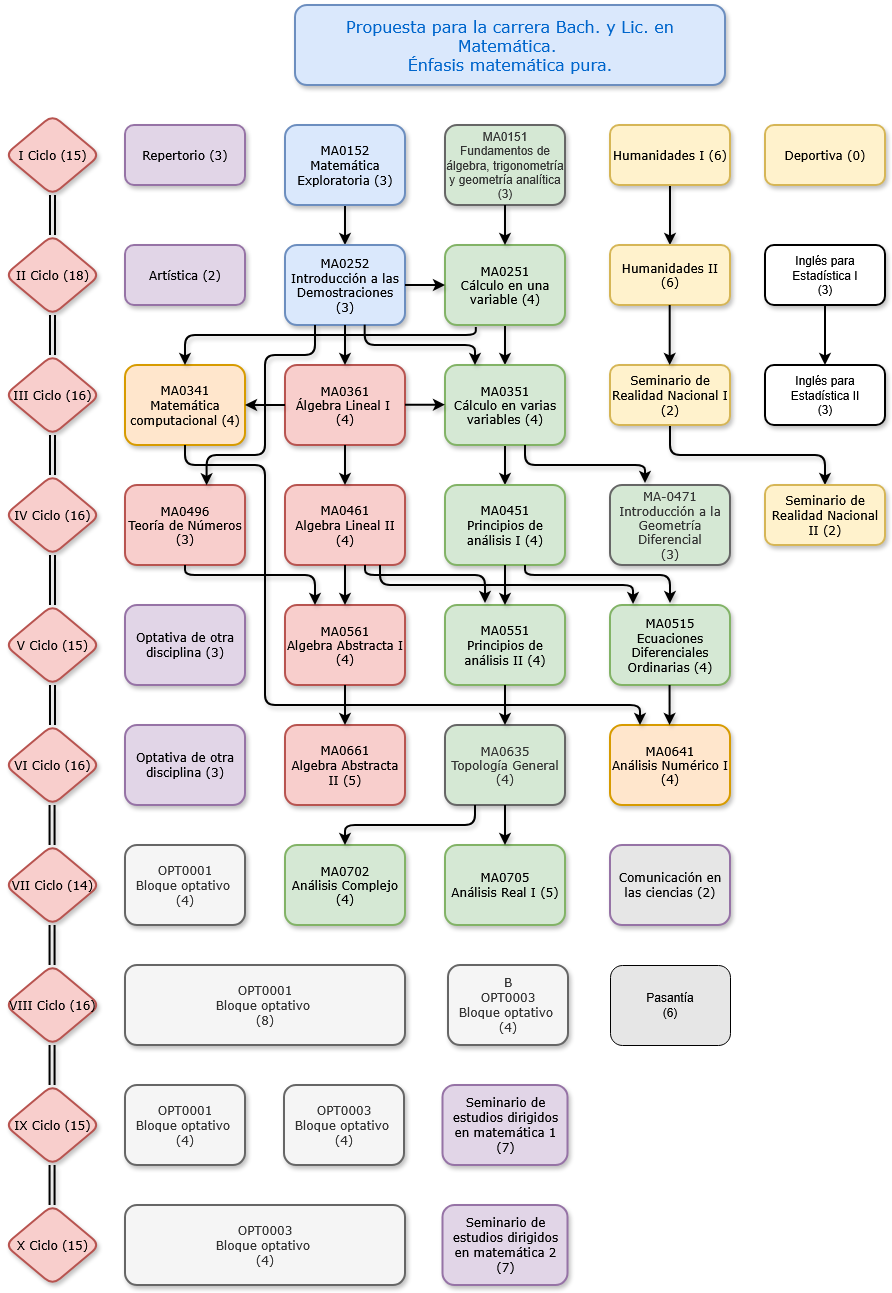
\includegraphics[width=0.75\textwidth]{propuesta_pura}
\caption{Diagrama de plan de Bachillerato y Licenciatura en Matemática con énfasis en Matemática Pura}
\end{figure}

\begin{figure}
\centering
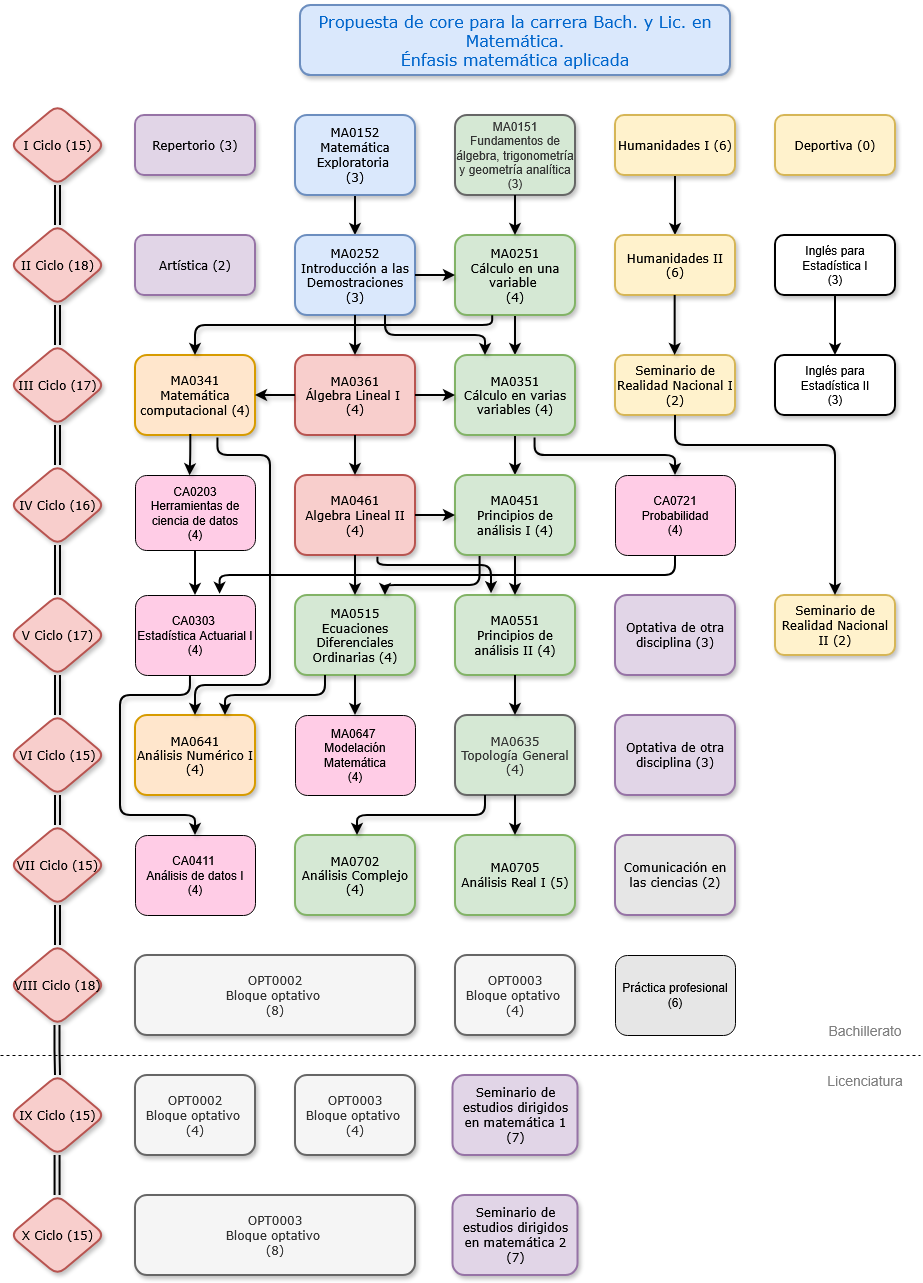
\includegraphics[width=0.75\textwidth]{propuesta_aplicada}
\caption{Diagrama de plan de Bachillerato y Licenciatura en Matemática con énfasis en Matemática Aplicada}
\end{figure}

\subsection{Requisitos de graduación}

\subsubsection{Bachillerato en matemática, ambos énfasis}

Se requiere de la asistencia, a lo largo de la carrera, a diez (10) actividades académicas válidas , por ejemplo:
\begin{enumerate}
    \item Charlas del Coloquio del Departamento de Matemáticas.
    \item Seminarios, conferencias o ciclos especiales anunciados por el departamento como válidos para este curso.
    \item Otras actividades académicas que la Dirección del Departamento disponga expresamente, con indicaciones oportunas.
\end{enumerate}

\subsubsection{Licenciatura en matemática, ambos énfasis}

Se requiere de la asistencia, a lo largo de la carrera, a cinco (5) actividades académicas válidas, distintas a las empleadas para cumplir el requerimiento similar de bachillerato, por ejemplo:
\begin{enumerate}
    \item Charlas del Coloquio del Departamento de Matemáticas.
    \item Seminarios, conferencias o ciclos especiales anunciados por el departamento como válidos para este curso.
    \item Otras actividades académicas que la Dirección del Departamento disponga expresamente, con indicaciones oportunas.
\end{enumerate}
\begin{refsection}
%\section{Selección de contenidos}

%En este capítulo se describe la metodología empleada en la selección de contenidos y cursos en la nueva propuesta de estructura curricular.



%\section{Reuniones con expertos por áreas disciplinares}

\section{Pertinencia de un bloque común en el plan de estudios}

Por las razones expuestas en la sección anterior, y con la idea de tener una mayor flexibilidad curricular en la carrera de Matemáticas, se plantea un bloque común (core) al inicio de la carrera, que permita explorar y estudiar diferentes áreas de la matemática posteriormente. Según la discusión que se planteó en la Reunión de Departamento del 05 de mayo de 2021, la planificación de la secuencia de los contenidos y las formas en las cuales se pueden organizar debe plantearse en función de las cinco áreas curriculares establecidas en el perfil de egreso: habilidades operacionales, pensamiento abstracto, formalismo, pensamiento algorítmico y habilidades investigativas. En el desarrollo de las capacidades cognitivas del estudiante, se definió iniciar con un enfoque operacional que disminuye progresivamente, mientras que conforme se van adquiriendo destrezas operacionales se va introduciendo y aumentando el nivel de abstracción y formalismo esperado. En paralelo, se deben ir desarrollando el pensamiento algorítmico y habilidades investigativas de forma creciente según el año de estudio.\\

De esta forma, en el core se busca suplir diferentes áreas del conocimiento que deben ser parte de una formación sólida de cualquier persona que desea ejercer como profesional en Matemática. En este proceso de aprendizaje, Bolaños (2015) recomienda que la secuencia de contenidos se puede organizar mediante cursos, módulos, talleres, seminarios y combinaciones de estos (p.11). Esta nueva forma de trabajar en la carrera permitirá establecer puntos en común según las exigencias y necesidades del Departamento de Matemática.

En el perfil de egreso se estableció que

\begin{center}
\begin{minipage}{0.75\linewidth}
        \vspace{5pt}%margen superior de minipage
        {\small
                Los primeros ciclos de la carrera deberán contener una alta proporción de aprendizaje conductista, con pequeños matices de los enfoques cognitivo y crítico… En esta etapa temprana, el enfoque cognitivo puede irse implantando de manera paulatina mediante talleres y actividades lúdicas o de estudio independiente, incrustadas dentro de los cursos teórico-prácticos… Hacia la parte final de la carrera se busca que [la persona estudiante] realice cognitivamente los procesos de aprendizaje. (p.57-58).
        }
        \vspace{5pt}%margen inferior de la minipage
    \end{minipage}
\end{center}

Incluso, ya se había mencionado desde los espacios de reflexión previos que el estudiantado “lo primero que debe aprender no tiene que ver con los contenidos, es
necesario que aprenda formas de organizar el pensamiento en Matemática” (p. 60) (**Esta postura es la parte crucial para la comprensión de lo que se está haciendo en los cursos de primer año**). Esta es una visión que se comparte en el cuerpo docente y una forma de dar respuesta a esta pretensión es el establecimiento de un core en la etapa inicial de la formación en la carrera de Matemática.

Asimismo, después de la revisión de los programas de la carrera de Matemática en diferentes universidades del mundo (UNAM, MIT, UChicago, Paris-Saclay, por mencionar solo algunas), se evidenció que esta forma de proponer un plan de estudio es una práctica usual, por lo que se reflexionó acerca de la pertinencia para adoptar prácticas similares en nuestra universidad. 

Este bloque común debe permitir un desempeño favorable en diferentes énfasis o áreas de especialización. Esto va acorde con la renovación y actualización del cuerpo docente, y con la diversificación de intereses de investigación, lo que permite una amplia gama de posibilidades para el estudiantado.

\section{Áreas curriculares}

La presente sección tiene por finalidad dar una definición a las distintas áreas curriculares presentadas en la Propuesta para el rediseño del Bachillerato en Matemática. Antes que nada, conviene definir qué se entenderá por áreas curriculares. Según el Artículo 2 del Acuerdo 033 del Consejo Superior Universitario del 2007, las áreas curriculares son “conjunto de programas curriculares afines que pueden ser agrupados porque sus referentes epistemológicos pertenecen a un área común de conocimiento” (Artículo 2 del Acuerdo 033 del Consejo Superior Universitario, 2007). Por su parte, un programa curricular

\begin{center}
\begin{minipage}{0.8\linewidth}
        \vspace{5pt}%margen superior de minipage
        {\small
                Es un sistema abierto y dinámico compuesto por actividades, procesos, recursos, infraestructura, profesores, estudiantes, egresados, mecanismos de evaluación y estrategias de articulación con la sociedad, mediante el cual se desarrolla un proceso que busca cumplir ciertos objetivos de formación en los estudiantes a través de sus planes de estudio. El título académico es el reconocimiento que hace la sociedad, a través de la Universidad, del cumplimiento de dichos objetivos de formación por parte de un individuo. (Artículo 3 del Acuerdo 033 del Consejo Superior Universitario, 2007).
        }
        \vspace{5pt}%margen inferior de la minipage
    \end{minipage}
\end{center}


En esta sección se describen las áreas curriculares según el análisis realizado en el perfil de egreso y la reunión de departamento efectuada el 05 de mayo de 2021.

\begin{table}[H]
\begin{center}
\begin{tabular}{|lccc|}
\hline
\multicolumn{4}{|c|}{\cellcolor[HTML]{00C0F3} \textbf{Habilidades operacionales}} \\ \hline
\multicolumn{1}{|l|}{} & \multicolumn{1}{c|}{\cellcolor[HTML]{8ED8F8} \textbf{Año}} & \multicolumn{1}{c|}{\cellcolor[HTML]{8ED8F8} \textbf{Dominio}} & \cellcolor[HTML]{8ED8F8} \textbf{Contenidos} \\ \cline{2-4} 
\multicolumn{1}{|l|}{} & \multicolumn{1}{c|}{I} & \multicolumn{1}{c|}{Alto} & Alto \\ \cline{2-4} 
\multicolumn{1}{|l|}{} & \multicolumn{1}{c|}{II} & \multicolumn{1}{c|}{Alto} & Medio \\ \cline{2-4} 
\multicolumn{1}{|l|}{} & \multicolumn{1}{c|}{III} & \multicolumn{1}{c|}{Alto} & Bajo \\ \cline{2-4} 
\multicolumn{1}{|l|}{\multirow{-5}{*}{\begin{tabular}[c]{@{}l@{}}Conjunto de todas las destrezas que requiere la persona \\ estudiante para poder efectuar operaciones matemáticas\\ concretas de cierta temática (aritmética, funciones, teoría\\  de conjuntos, cálculo, probabilidad, etc,), en la que no \\ es necesario un pensamiento abstracto. \end{tabular}}} & \multicolumn{1}{c|}{IV} & \multicolumn{1}{c|}{Alto} & Bajo \\ \hline
\end{tabular}
\end{center}
\end{table}

\begin{table}[H]
\begin{center}
\begin{tabular}{|llll|}
\hline
\multicolumn{4}{|c|}{\cellcolor[HTML]{00C0F3} \textbf{Pensamiento Abstracto}} \\ \hline
\multicolumn{1}{|l|}{} & \multicolumn{1}{l|}{\cellcolor[HTML]{8ED8F8}} & \multicolumn{1}{l|}{\cellcolor[HTML]{8ED8F8}} & \cellcolor[HTML]{8ED8F8} \\
\multicolumn{1}{|l|}{} & \multicolumn{1}{l|}{\cellcolor[HTML]{8ED8F8}} & \multicolumn{1}{l|}{\cellcolor[HTML]{8ED8F8}} & \cellcolor[HTML]{8ED8F8} \\
\multicolumn{1}{|l|}{} & \multicolumn{1}{l|}{\multirow{-3}{*}{\cellcolor[HTML]{8ED8F8} \textbf{Año}}} & \multicolumn{1}{l|}{\multirow{-3}{*}{\cellcolor[HTML]{8ED8F8} \textbf{Dominio}}} & \multirow{-3}{*}{\cellcolor[HTML]{8ED8F8} \textbf{Contenidos}} \\ \cline{2-4} 
\multicolumn{1}{|l|}{} & \multicolumn{1}{l|}{I} & \multicolumn{1}{l|}{Medio} & Bajo \\ \cline{2-4} 
\multicolumn{1}{|l|}{} & \multicolumn{1}{l|}{II} & \multicolumn{1}{l|}{Medio} & Medio \\ \cline{2-4} 
\multicolumn{1}{|l|}{} & \multicolumn{1}{l|}{III} & \multicolumn{1}{l|}{Alto} & Alto \\ \cline{2-4} 
\multicolumn{1}{|l|}{\multirow{-7}{*}{\begin{tabular}[c]{@{}l@{}}- Nivel elevado del pensamiento en el cual convergen la\\ deducción, la síntesis, la interpretación y el análisis.\\ - Medio para la construcción del conocimiento teórico a\\ través del proceso de formación del concepto.\\ - Supone la capacidad de asumir un marco mental de \\ trabajo, en el que necesariamente se tengan claros muchos\\ conceptos para poder generar más conocimiento teórico.\end{tabular}}} & \multicolumn{1}{l|}{IV} & \multicolumn{1}{l|}{Alto} & Alto \\ \hline
\end{tabular}
\end{center}
\end{table}

\begin{table}[H]
\begin{center}
\begin{tabular}{|llll|}
\hline
\multicolumn{4}{|c|}{\cellcolor[HTML]{00C0F3} \textbf{Pensamiento Algorítmico}} \\ \hline
\multicolumn{1}{|l|}{} & \multicolumn{1}{l|}{\cellcolor[HTML]{8ED8F8} \textbf{Año}} & \multicolumn{1}{l|}{\cellcolor[HTML]{8ED8F8} \textbf{Dominio}} & \cellcolor[HTML]{8ED8F8} \textbf{Contenidos} \\ \cline{2-4} 
\multicolumn{1}{|l|}{} & \multicolumn{1}{l|}{I} & \multicolumn{1}{l|}{Bajo} & Bajo \\ \cline{2-4} 
\multicolumn{1}{|l|}{} & \multicolumn{1}{l|}{II} & \multicolumn{1}{l|}{Medio} & Medio \\ \cline{2-4} 
\multicolumn{1}{|l|}{} & \multicolumn{1}{l|}{III} & \multicolumn{1}{l|}{Alto} & Alto \\ \cline{2-4} 
\multicolumn{1}{|l|}{\multirow{-5}{*}{\begin{tabular}[c]{@{}l@{}}Capacidad de entender, ejecutar, evaluar y\\ crear algoritmos. El pensamiento que hace \\ uso de procesos recursivos.\end{tabular}}} & \multicolumn{1}{l|}{IV} & \multicolumn{1}{l|}{Alto} & Alto \\ \hline
\end{tabular}
\end{center}
\end{table}

\begin{table}[H]
\begin{center}
\begin{tabular}{|llll|}
\hline
\multicolumn{4}{|c|}{\cellcolor[HTML]{00C0F3} \textbf{Formalismo}} \\ \hline
\multicolumn{1}{|l|}{} & \multicolumn{1}{l|}{\cellcolor[HTML]{8ED8F8} \textbf{Año}} & \multicolumn{1}{l|}{\cellcolor[HTML]{8ED8F8} \textbf{Dominio}} & \cellcolor[HTML]{8ED8F8}\textbf{Contenidos} \\ \cline{2-4} 
\multicolumn{1}{|l|}{} & \multicolumn{1}{l|}{I} & \multicolumn{1}{l|}{Bajo} & Bajo \\ \cline{2-4} 
\multicolumn{1}{|l|}{} & \multicolumn{1}{l|}{II} & \multicolumn{1}{l|}{Medio} & Medio \\ \cline{2-4} 
\multicolumn{1}{|l|}{} & \multicolumn{1}{l|}{III} & \multicolumn{1}{l|}{Alto} & Medio \\ \cline{2-4} 
\multicolumn{1}{|l|}{\multirow{-5}{*}{\begin{tabular}[c]{@{}l@{}}Implica que el estudiantado pueda estructurar de tal manera el\\  pensamiento para poderlo comunicar de una forma que se \\ ajuste a las reglas de legitimación matemáticas establecidas. \\ Si bien es cierto, el formalismo no es lo que mueve a un \\ matemático, si que es algo de lo que no se puede prescindir.\end{tabular}}} & \multicolumn{1}{l|}{IV} & \multicolumn{1}{l|}{Alto} & Alto \\ \hline
\end{tabular}
\end{center}
\end{table}

\begin{table}[H]
\begin{center}
\begin{tabular}{|llll|}
\hline
\multicolumn{4}{|c|}{\cellcolor[HTML]{00C0F3} \textbf{Habilidades investigativas}} \\ \hline
\multicolumn{1}{|l|}{} & \multicolumn{1}{l|}{\cellcolor[HTML]{8ED8F8}} & \multicolumn{1}{l|}{\cellcolor[HTML]{8ED8F8}} & \cellcolor[HTML]{8ED8F8} \\
\multicolumn{1}{|l|}{} & \multicolumn{1}{l|}{\multirow{-2}{*}{\cellcolor[HTML]{8ED8F8} \textbf{Año}}} & \multicolumn{1}{l|}{\multirow{-2}{*}{\cellcolor[HTML]{8ED8F8} \textbf{Dominio}}} & \multirow{-2}{*}{\cellcolor[HTML]{8ED8F8} \textbf{Contenidos}} \\ \cline{2-4} 
\multicolumn{1}{|l|}{} & \multicolumn{1}{l|}{} & \multicolumn{1}{l|}{} &  \\
\multicolumn{1}{|l|}{} & \multicolumn{1}{l|}{\multirow{-2}{*}{I}} & \multicolumn{1}{l|}{\multirow{-2}{*}{-}} & \multirow{-2}{*}{Bajo} \\ \cline{2-4} 
\multicolumn{1}{|l|}{} & \multicolumn{1}{l|}{} & \multicolumn{1}{l|}{} &  \\
\multicolumn{1}{|l|}{} & \multicolumn{1}{l|}{\multirow{-2}{*}{II}} & \multicolumn{1}{l|}{\multirow{-2}{*}{-}} & \multirow{-2}{*}{Bajo} \\ \cline{2-4} 
\multicolumn{1}{|l|}{} & \multicolumn{1}{l|}{} & \multicolumn{1}{l|}{} &  \\
\multicolumn{1}{|l|}{} & \multicolumn{1}{l|}{\multirow{-2}{*}{III}} & \multicolumn{1}{l|}{\multirow{-2}{*}{Bajo}} & \multirow{-2}{*}{Bajo} \\ \cline{2-4} 
\multicolumn{1}{|l|}{} & \multicolumn{1}{l|}{} & \multicolumn{1}{l|}{} &  \\
\multicolumn{1}{|l|}{\multirow{-10}{*}{\begin{tabular}[c]{@{}l@{}}Conjunto de habilidades de diversa naturaleza, que empiezan \\ a desarrollarse desde antes de que el individuo tenga acceso a\\ procesos sistemáticos de formación para la investigación, que\\ en su mayoría no se desarrollan solo para posibilitar la \\ realización de las tareas propias de la investigación, pero que \\ han sido detectadas por formadores como habilidades cuyo \\ desarrollo. en el(la) investigador(a) en formación o en \\ funciones, es una contribución fundamental para potenciar \\ que pueda realizar investigación de buena calidad.\end{tabular}}} & \multicolumn{1}{l|}{\multirow{-2}{*}{IV}} & \multicolumn{1}{l|}{\multirow{-2}{*}{Medio}} & \multirow{-2}{*}{Medio} \\ \hline
\end{tabular}
\end{center}
\end{table}

\section{Lógica de selección de contenidos}

La selección de contenidos responde a una lógica de construcción que inició con la identificación del objeto de estudio, se moldea con los saberes, competencias y valores del perfil de egreso determinados a partir de la recopilación de información contextual de la carrera, y que se termina de pulir con el aporte de profesionales y docentes.

Con base en la recopilación de información que se hizo en los talleres y asignaciones de inicio del 2021, se reportan las subáreas de contenidos con una puntuación mayor o igual que 1 (en una escala de 0 a 3) con base en las respuestas obtenidas para los dos primeros años; ver Tablas 4, 5, 6 y 7. Según se indicó, la nota brindada indica el nivel que cada contenido aporta a la consecución del área curricular correspondiente.

\begin{table}[H]
\begin{center}
\caption{Puntajes obtenidos para el primer año con calificación mayor o igual a 1. Las entradas vacías son cero}
\label{Primeranno}
\end{center}
\begin{center}
\begin{tabular}{|l|c|c|c|c|}
\hline
\rowcolor[HTML]{00C0F3} 
\multicolumn{1}{|c|}{\cellcolor[HTML]{00C0F3} \textbf{Contenidos}} & \textbf{Oper} & \textbf{Abs} & \textbf{Form} & \textbf{Alg} \\ \hline
Demostraciones & 2.3 & 1.7 & 1.6 &  \\ \hline
Inducción & 2.7 & 1.1 & 1.3 & 1.4 \\ \hline
Lógica proposicional & 1.7 & 1.6 & 1.6 & 1.1 \\ \hline
Teoría de conjuntos & 1.8 & 1.5 & 1.6 &  \\ \hline
Combinatoria & 2.3 &  &  & 1.5 \\ \hline
Bases de programación & 1.5 &  &  & 1.3 \\ \hline
Precálculo & 2.5 & 1 & 1 & 1.3 \\ \hline
Cálculo & 2.2 &  &  & 1.3 \\ \hline
Álgebra lineal & 1.9 &  &  & 1.2 \\ \hline
Análisis complejo & 1.3 &  &  &  \\ \hline
Probabilidad & 1.4 &  &  &  \\ \hline
Estadística & 1.3 &  &  &  \\ \hline
Preliminares de álgebra & 2.3 & 1.5 & 1.2 & 1.5 \\ \hline
Álgebra lineal & 1.5 &  &  &  \\ \hline
Cuerpos & 1.0 &  &  &  \\ \hline
Divisibilidad factorización & 2.4 & 1.2 &  & 2.1 \\ \hline
Aritmética modular & 2.3 &  &  & 2.1 \\ \hline
Funciones aritméticas & 1.4 &  &  & 1.1 \\ \hline
Álgebras de Boole & 1.1 &  &  &  \\ \hline
Geometría Euclídea & 1.8 & 1.4 & 1.4 & 1.3 \\ \hline
Geometría analítica & 1.1 &  &  &  \\ \hline
\end{tabular}
\end{center}
\end{table}

Con respecto al primer año, se observa que los contenidos dominantes en el área de habilidades operaciones son temas del área de fundamentos (demostraciones, inducción, lógica proposicional, teoría de conjuntos, combinatoria), análisis (precálculo, cálculo), álgebra (álgebra lineal, preliminares de álgebra, cuerpos), teoría de números (divisibilidad, factorización, aritmética modular, funciones aritméticas) y geometría (geometría euclídea y analítica). Se plantea por tal razón tener un bloque de dos cursos introductorios que incluya estos temas, menos los contenidos de análisis que por los temas específicos se agruparan en dos cursos adicionales. En el área curricular del pensamiento algorítmico, dominan los contenidos de teoría de números, combinatoria, preliminares de álgebra, inducción, precálculo y cálculo, en los cuales se estudian algoritmos específicos que facilitan el desarrollo de dicha área

\begin{table}[H]
\begin{center}
\end{center}
\begin{center}
\begin{tabular}{|l|c|c|c|c|}
\hline
\rowcolor[HTML]{00C0F3} 
\multicolumn{1}{|c|}{\cellcolor[HTML]{00C0F3} \textbf{Contenidos}} & \textbf{Oper} & \textbf{Abs} & \textbf{Form} & \textbf{Alg} \\ \hline
Demostraciones & 1.5 & 2.1 & 2.4 &  \\ \hline
Inducción & 2 & 1.5 & 1.6 &  \\ \hline
Lógica proposicional & 1.2 & 1.4 & 1.5 &  \\ \hline
Teoría de conjuntos & 1.3 & 1.6 & 1.9 & 1 \\ \hline
Combinatoria & 1.6 & 1.5 & 1.1 & 1.4 \\ \hline
Bases de programación & 1.6 & 1.2 &  & 1.8 \\ \hline
Estructura de datos & 1.3 &  &  & 1.2 \\ \hline
Paradigmas computacionales & 1.1 &  &  & 1.1 \\ \hline
Bases de datos & 1.0 &  &  &  \\ \hline
Cálculo & 1.8 & 1.9 & 2.1 & 1.5 \\ \hline
Álgebra lineal & 2.1 & 2.4 & 2.2 & 1.9 \\ \hline
Espacios métricos & 1.3 & 1.1 & 1.1 &  \\ \hline
Ánalisis real & 1.3 & 1.2 & 1.2 &  \\ \hline
Análisis complejo & 1.3 &  &  &  \\ \hline
Probabilidad & 1.3 &  &  &  \\ \hline
Estadística & 1.4 &  &  & 1.1 \\ \hline
Análisis numérico & 1.3 &  &  & 1.4 \\ \hline
ODEs & 1.6 &  &  &  \\ \hline
Preliminares de álgebra & 1.3 & 1.5 & 1.7 & 1.3 \\ \hline
Álgebra lineal & 1.8 & 2.0 & 1.8 & 1.5 \\ \hline
Grupos & 1.2 & 1.1 & 1.2 &  \\ \hline
Anillos & \multicolumn{1}{l|}{1.1} & \multicolumn{1}{l|}{1.1} & \multicolumn{1}{l|}{1.2} & \multicolumn{1}{l|}{} \\ \hline
Cuerpos & \multicolumn{1}{l|}{1.1} & \multicolumn{1}{l|}{1.1} & \multicolumn{1}{l|}{1.2} & \multicolumn{1}{l|}{} \\ \hline
Espacios vectoriales & \multicolumn{1}{l|}{2.0} & \multicolumn{1}{l|}{2.3} & \multicolumn{1}{l|}{2.3} & \multicolumn{1}{l|}{1.1} \\ \hline
Geometría Euclídea & \multicolumn{1}{l|}{1.0} & \multicolumn{1}{l|}{1.2} & \multicolumn{1}{l|}{1.4} & \multicolumn{1}{l|}{} \\ \hline
Geometría analítica & \multicolumn{1}{l|}{1.4} & \multicolumn{1}{l|}{} & \multicolumn{1}{l|}{} & \multicolumn{1}{l|}{} \\ \hline
Topología (esp. Euclídeo) & \multicolumn{1}{l|}{1.3} & \multicolumn{1}{l|}{1.4} & \multicolumn{1}{l|}{1.2} & \multicolumn{1}{l|}{} \\ \hline
Topología (esp. métricos) & \multicolumn{1}{l|}{1.2} & \multicolumn{1}{l|}{1.1} & \multicolumn{1}{l|}{} & \multicolumn{1}{l|}{} \\ \hline
\end{tabular}
\end{center}
\caption{Puntajes obtenidos para el segundo año con calificación mayor o igual a 1. Las entradas vacías son cero}
\end{table}

En el caso del segundo año, en donde se espera un incremento en las áreas de pensamiento algorítmico, formalismo y pensamiento abstracto, se obtuvo una alta calificación en los temas de demostraciones, cálculo, álgebra lineal, espacios vectoriales, teoría de conjuntos e inducción.

\begin{table}[H]
\begin{center}
\end{center}
\begin{center}
\begin{tabular}{|l|c|c|c|c|}
\hline
\rowcolor[HTML]{00C0F3} 
\multicolumn{1}{|c|}{\cellcolor[HTML]{00C0F3} \textbf{Contenidos}} & \textbf{Oper}& \textbf{Abs} & \textbf{Form} & \textbf{Alg} \\ \hline
Demostraciones &  & 1.5 & 1.5 &  \\ \hline
Lógica proposicional &  &  &  & 1 \\ \hline
Combinatoria & 1.2 & 1 &  & 1.1 \\ \hline
Bases de programación & 1.6 & 1.2 &  & 1.8 \\ \hline
Estructura de datos & 1.5 &  &  & 1.3 \\ \hline
Paradigmas computacionales & 1 & 1 &  & 1 \\ \hline
Bases de datos & 1.1 &  &  & 1.1 \\ \hline
Aprendizaje automático & 1.2 &  &  & 1.3 \\ \hline
Espacios métricos & 1.1 & 2.3 & 1.9 &  \\ \hline
Ánalisis real & 1.2 & 2.4 & 2.0 &  \\ \hline
Análisis complejo & 1.5 & 2 & 1.8 &  \\ \hline
Probabilidad & 1.3 & 1.8 & 1.2 & 1.0 \\ \hline
Estadística & 1.5 & 1.2 & 1.3 & 1.3 \\ \hline
Análisis numérico & 1.9 & 1.3 & 1.3 & 2.3 \\ \hline
Análisis funcional &  & 1.6 & 1.3 &  \\ \hline
ODEs & 1.5 & 2.3 & 2.1 & 1.6 \\ \hline
PDEs & 1.6 & 1.1 & 1.1 & 1.3 \\ \hline
Modelación  matemática & 1.2 & 1.1 &  & 1.1 \\ \hline
Grupos & 1.8 & 2.8 & 2.1 & 1.6 \\ \hline
Anillos & 1.9 & 2.8 & 1.22.2 & 1.7 \\ \hline
Cuerpos & 1.7 & 2.7 & 2.1 & 1.4 \\ \hline
Álgebras & 1.3 & 2.1 & 1.8 &  \\ \hline
Módulos & 1.0 & 1.8 & 1.8 &  \\ \hline
Teoría de Galois & 1.9 & 2.6 & 2.2 & 2.1 \\ \hline
Teoría de códigos & 1.3 & 1.1 &  &  \\ \hline
Curvas elípticas &  & 1.1 &  &  \\ \hline
Álgebra de Boole &  & 1.0 & 1.0 &  \\ \hline
Cálculo de predicados & 1.6 & 1.5 & 1.5 & 1.0 \\ \hline
Teoría de Computabilidad & 1.1 & 1.2 & 1.1 & 1.2 \\ \hline
Teoría de Modelos & 1.4 & 1.3 & 1.4 &  \\ \hline
Teoría de Demostración & 1.0 & 1.2 & 1.2 &  \\ \hline
Geometría proyectiva &  & 1.5 & 1.4 &  \\ \hline
Geometría diferencial & 1.0 & 1.0 &  &  \\ \hline
Topología de espacios euclídeos & 1.4 & 1.7 & 1.5 &  \\ \hline
Topología de espacios métricos & 1.5 & 2.1 & 2.0 &  \\ \hline
Topología general & 1.4 & 2.0 & 1.8 &  \\ \hline
\end{tabular}
\end{center}
\caption{Puntajes obtenidos para el tercer año con calificación mayor o igual a 1. Las entradas vacías son cero.}
\end{table}

Para el tercer año, en pensamiento abstracto y formalismo dominan los contenidos de espacios métricos, análisis real y complejo, probabilidad, ecuaciones diferenciales ordinarias, grupos, anillos, cuerpos, álgebras, teoría de Galois, cálculo de predicados, geometría proyectiva y topología. En el pensamiento algorítmico destacan análisis numérico, programación, teoría de Galois y álgebra.

\begin{table}[H]
\begin{center}
\end{center}
\begin{center}
\begin{tabular}{|l|c|c|c|c|}
\hline
\rowcolor[HTML]{00C0F3} 
\multicolumn{1}{|c|}{\cellcolor[HTML]{00C0F3} \textbf{Contenidos}} & \textbf{Oper} & \textbf{Abs} & \textbf{Form} & \textbf{Alg} \\ \hline
Bases de programación & 1.0 &  &  & 1.1 \\ \hline
Aprendizaje automático &  &  &  & 1.0 \\ \hline
Espacios métricos &  & 1.6 & 1.4 &  \\ \hline
Análisis real & 1.1 & 2.3 & 2.0 & 1.0 \\ \hline
Análisis complejo & 1.1 & 1.6 & 1.5 &  \\ \hline
Probabilidad & 1.3 & 2.2 & 1.6 & 1.5 \\ \hline
Estadística & 1.0 & 1.5 & 1.3 & 1.1 \\ \hline
Análisis numérico & 1.4 & 1.2 & 1.5 & 2.0 \\ \hline
Análisis funcional &  & 2.1 & 1.7 &  \\ \hline
PDEs & 1.2 & 2.3 & 2.0 & 1.5 \\ \hline
Análisis armónico & 1.4 & 1.7 & 1.4 & 1.3 \\ \hline
Modelación matemática & 1.5 & 1.4 & 1.3 & 1.7 \\ \hline
Grupos &  & 1.4 & 1.4 &  \\ \hline
Anillos &  & 1.0 & 1.0 &  \\ \hline
Cuerpos &  & 1.0 & 1.0 &  \\ \hline
Álgebras & 1.2 & 1.9 & 1.6 & 1.0 \\ \hline
Módulos & 1.3 & 1.9 & 1.5 & 1.0 \\ \hline
Teoría de Galois &  & 1.0 &  &  \\ \hline
Álgebra homológica & 1.7 & 2.4 & 2.0 & 1.5 \\ \hline
Teoría de códigos &  & 1.1 &  &  \\ \hline
Teoría de autómatas &  & 1.1 &  &  \\ \hline
Criptografía de la llave pública & 1.0 &  &  & 1.0 \\ \hline
Curvas elípticas & 1.4 & 1.8 & 1.1 & 1.8 \\ \hline
Criptografía avanzada & 1.9 & 1.3 & 1.0 & 2.7 \\ \hline
Teoría analítica de números & 1.3 & 1.6 & 1.2 &  \\ \hline
Teoría de Computabilidad & 1.4 & 2.4 & 2.2 & 1.1 \\ \hline
Teoría de Modelos & 1.7 & 2.5 & 2.5 & 1.0 \\ \hline
Teoría de Demostración & 1.5 & 1.8 & 1.7 &  \\ \hline
Teoría descriptiva de conjuntos (ZF/ZFC) & 1.3 & 2.0 & 1.9 &  \\ \hline
Geometría proyectiva &  & 1.2 & 1.2 &  \\ \hline
Geometría diferencial & 1.7 & 2.1 & 1.8 &  \\ \hline
Geometría algebraica & 1.9 & 2.6 & 2.2 & 1.2 \\ \hline
Topología de espacios euclídeos &  & 1.0 &  &  \\ \hline
Topología de espacios métricos &  &  &  &  \\ \hline
Topología general &  & 1.6 & 1.2 &  \\ \hline
Homotopía & 1.7 & 2.8 & 2.3 & 1.1 \\ \hline
Homología & 1.6 & 2.7 & 2.3 &  \\ \hline
\end{tabular}
\end{center}
\caption{Puntajes obtenidos para el cuarto año con calificación mayor o igual a 1. Las entradas vacías son cero.}
\end{table}

Para el cuarto año, existe una mayor diversidad en temas sugeridos para el desarrollo de las áreas de pensamiento abstracto, algorítmico y formalismo. En general, destacan análisis real, probabilidad, análisis funcional, ecuaciones en derivadas parciales, álgebra homológica, teoría de computabilidad, teoría de modelos, teoría de conjuntos, geometría diferencial, geometría algebraica, homotopía y homología.

\section{Organización}

A continuación se describe la lógica en la organización de los cursos de la estructura curricular propuesta. De acuerdo con los criterios de organización y secuencia de contenidos, los cursos se agrupan por elementos en común ---las cinco áreas curriculares definidas en el perfil de egreso: habilidades operacionales, pensamiento abstracto, formalismo, pensamiento algorítmico y habilidades investigativas--- y se disponen en una secuencia vertical (por años y ciclos) y horizontal (dentro de un mismo ciclo lectivo), de modo que se garantice continuidad e integración entre las actividades formativas.

La organización sigue un diseño con tronco común en los primeros ciclos y, a partir del segundo año, el énfasis en matemática pura y el énfasis en matemática aplicada. En el desarrollo de las capacidades cognitivas se inicia con un enfoque operacional que disminuye progresivamente, mientras que el nivel de abstracción, formalismo y pensamiento algorítmico aumenta conforme avanza la carrera; las habilidades investigativas se refuerzan de forma transversal y se concentran con mayor intensidad en los últimos ciclos. Esta disposición gradual y armónica busca que el estudiantado logre una mejor comprensión y mayor profundización, conforme a lo establecido en la normativa universitaria y en los lineamientos de CONARE para la secuencia curricular.

\subsection{Cursos con énfasis operacional}

Con base en los niveles propuestos de las áreas curriculares, el primer año concentra el énfasis operacional, con dominio y contenidos altos en esta área. Se pretende así satisfacer las necesidades de los cursos posteriores y permitir una transición acorde con el perfil de ingreso y la madurez matemática del estudiantado. Si bien estos cursos tienen un alto componente operacional ---tanto en contenidos como en el dominio esperado---, también incorporan, de manera inicial, aspectos de pensamiento abstracto. La evaluación privilegia la habilidad operacional, y los contenidos sirven de introducción, en la medida de lo posible, al pensamiento abstracto y al formalismo.

En el ciclo I se ubican MA-0151 Fundamentos de álgebra, trigonometría y geometría analítica y MA-0152 Matemática Exploratoria. El primero desarrolla destrezas operacionales e intuición geométrica sobre álgebra, trigonometría y geometría vectorial y analítica, priorizando ejemplos concretos. El segundo inicia al estudiantado en el razonamiento inductivo y deductivo mediante resolución de problemas, con exploraciones en objetos discretos (teoría de números, combinatoria) y primeras nociones de pruebas sencillas de carácter operacional.

En el ciclo II, MA-0251 Introducción al Cálculo en una variable continúa el énfasis operacional e intuitivo sobre límites, derivadas e integrales, con trabajo centrado en ejemplos concretos y técnicas de cálculo. 

En el segundo año se mantiene un componente operacional alto en dominio, aunque los contenidos operacionales pasan a un nivel medio. MA-0361 Álgebra Lineal I enfatiza habilidades operacionales e intuición geométrica (sistemas, matrices, determinantes), e introduce progresivamente abstracción y formalismo mediante espacios vectoriales y transformaciones lineales. MA-0351 Cálculo en varias variables prioriza igualmente la práctica, la intuición y el pensamiento geométrico sobre sucesiones, series y cálculo diferencial e integral en varias variables. En cursos posteriores el componente operacional no desaparece, pero resulta secundario frente al énfasis en abstracción, formalismo, pensamiento algorítmico o investigación, según lo descrito en las áreas curriculares.

\subsection{Cursos con énfasis en pensamiento algorítmico}

El pensamiento algorítmico se incorpora de forma creciente: bajo en el primer año, medio en el segundo y alto a partir del tercero. Se contempla la inclusión de cursos relacionados con el uso de tecnologías y la implementación de algoritmos, en aras de una formación alineada con el perfil de egreso y con las prácticas emergentes (ciencia de datos, computación científica, modelación), con contenidos actualizados según los requerimientos de la matemática en distintas áreas.

En el tronco común, MA-0341 Matemática Computacional (tercer ciclo) orienta el trabajo a implementar pensamiento algorítmico mediante programación en un lenguaje de alto nivel, retomando contenidos de demostraciones, cálculo y álgebra lineal para ejecutar, analizar y explorar algoritmos, priorizando la intuición y la implementación sobre el formalismo. En el sexto ciclo, MA-0641 Análisis Numérico I profundiza en la resolución de problemas mediante métodos numéricos, con análisis de error, eficiencia, convergencia e implementación, y propicia habilidades investigativas a través de búsqueda bibliográfica e implementación de métodos aplicados.

En el énfasis en matemática aplicada, CA-0203 Herramientas de ciencia de datos I desarrolla destrezas algorítmicas y tecnológicas (hojas de cálculo, R, \LaTeX{}, Markdown, control de versiones), y MA-0647 Modelación Matemática integra algoritmos, simulación y validación de modelos. Asimismo, cursos del tronco o de los énfasis incorporan componentes algorítmicos puntuales ---por ejemplo, experimentación computacional en álgebra lineal o implementación de algoritmos en teoría de números--- sin que ese sea su eje principal. Las optativas de núcleo y temáticas en análisis numérico, computación científica, aprendizaje automático, optimización y análisis de datos permiten profundizar este énfasis en el cuarto año.

\subsection{Cursos con énfasis en pensamiento abstracto y formalismo}

En paralelo con lo anterior, en el primer año se incluye MA-0252 Introducción a las Demostraciones opera como puente entre la matemática predominantemente operacional y la más formal: retoma las intuiciones de exploración del primer ciclo y las articula con lógica, conjuntos, relaciones, funciones, teoría de números elemental e inducción, para desarrollar habilidades de demostración.

El pensamiento abstracto y el formalismo se introducen de forma paulatina y se consolidan a partir del segundo año (niveles medios), hasta alcanzar dominio y contenidos altos en el tercero y el cuarto. Los cursos de esta línea exigen estructurar el pensamiento conforme a las reglas de legitimación matemáticas, demostrar resultados y comunicar argumentos con rigor.

En el tronco común del segundo año, MA-0451 Principios de análisis I formaliza el análisis en una variable real (completitud, convergencia, diferenciación), asumiendo las intuiciones y destrezas operacionales de los cursos de cálculo y las bases de demostración del primer año. MA-0461 Álgebra Lineal II eleva el nivel de abstracción y formalismo (producto interno, teoría espectral, forma de Jordan), con demostraciones y resolución de problemas teóricos. En el tercer año, MA-0551 Principios de Análisis II continúa la formalización del análisis en varias variables; MA-0515 Ecuaciones Diferenciales aporta el sustento teórico de las ecuaciones ordinarias; y MA-0635 Topología General ofrece un tratamiento riguroso de espacios métricos y topológicos, continuidad, compacidad, conexidad y nociones de homotopía.

En el énfasis en matemática pura, MA-0496 Teoría de Números y MA-0471 Introducción a la Geometría Diferencial refuerzan demostración, abstracción y puente hacia estructuras algebraicas y geométricas más generales; MA-0561 Álgebra Abstracta I y MA-0661 Álgebra Abstracta II profundizan en anillos, módulos, grupos, cuerpos y teoría de Galois. En el cuarto año, cursos como MA-0702 Análisis Complejo y MA-0705 Análisis Real I consolidan el formalismo y la abstracción propios del análisis avanzado. En el énfasis en matemática aplicada, aunque el eje no es exclusivamente formalista, se exige dominio conceptual sólido (por ejemplo en probabilidad, estadística y modelación) que articula abstracción con transferencia a problemas concretos.

\subsection{Habilidades investigativas}

Según se externó por varios y varias docentes en la reunión de departamento efectuada el 05 de mayo de 2021, las habilidades investigativas deben estar presentes de forma transversal durante toda la carrera. A modo de ejemplo, en dicha reunión se sugirió asignar trabajos sobre temas relacionados con los cursos, búsquedas bibliográficas, proyectos, videos, búsquedas en internet, referenciar y citar, realizar bibliografías, asistencia a charlas y coloquios, exposiciones, entre otros. Esto no implica estudiar temas adicionales, sino abordar temas propios de los cursos mediante tareas que desarrollen las habilidades investigativas.

En la estructura propuesta, estas habilidades pasan de un nivel bajo en los primeros años a medio en el cuarto. De manera transversal, los programas de cursos del tronco y de los énfasis incorporan proyectos cortos, indagación bibliográfica, experimentación con software y comunicación oral o escrita de resultados. De forma específica, en los últimos ciclos se concentran actividades de formación orientadas a la práctica investigativa y profesional: MA-0780 Comunicación en las ciencias desarrolla escritura y expresión oral científica, ética y conducta responsable en investigación; y MA-0781 Práctica profesional en matemática pura o MA-0781 Práctica profesional en matemática aplicada permiten integrar conocimientos en un entorno académico (práctica de investigación) o profesional (aplicación en entes externos). En el énfasis en matemática aplicada, MA-0647 Modelación Matemática culmina con un proyecto de modelación que articula formulación, análisis, simulación y comunicación de resultados.

\subsection{Cursos optativos}

Los cursos optativos se organizan para ampliar la flexibilidad curricular respecto del plan vigente ---en el cual solo tres cursos optativos de matemática resultaban insuficientes frente al perfil de egreso--- y se agrupan en dos categorías: optativas de núcleo, con programas fijos en áreas representativas del objeto de estudio (análisis, álgebra, geometría, topología, probabilidad, estadística, lógica, optimización, sistemas dinámicos, entre otras), y optativas temáticas, que incluyen cursos de «Tópicos de\ldots» con contenidos abiertos por oferta según la especialidad docente y las necesidades formativas.

La oferta optativa es sustancialmente mayor que la del plan actual y se articula con el énfasis en matemática pura y el énfasis en matemática aplicada: en el primero predominan profundizaciones disciplinares teóricas; en el segundo se incluyen, además, opciones vinculadas a modelación, computación científica, análisis de datos, aprendizaje automático y, cuando corresponda, cursos de otras disciplinas afines que permitan trabajo interdisciplinario. De este modo, la organización de optativas refleja tanto la representatividad del campo disciplinar como la transferencia hacia contextos académicos y productivos contemplados en el perfil de egreso.

Los cursos optativos se dividen en dos tipos:
\begin{itemize}
    \item Optativos núcleo: Son aquellos cursos que, si bien son considerados optativos a un nivel de bachillerato o licenciatura, forman parte de temas que son ejes fundamentales en estudios más avanzados de matemática.
    \item Optativos temáticos: Se refiere a cursos que exploran temas que aunque sean importantes dentro de la disciplina no representan ejes fundamentales para estudios posteriores.
\end{itemize}

\printbibliography[heading=subbibliography,section=\the\value{refsection}]
\end{refsection}


\chapter{Elementos pedagógicos y programas de los cursos}
\chapter{Elementos pedagógicos y programas de los cursos}


\section{Análisis pedagógico}

En este apartado se presenta la caracterización del marco pedagógico que se considera viable para la carrera de Matemática, al tomar en cuenta cuáles aspectos se deben privilegiar por cada enfoque pedagógico y al considerar el aporte de las experiencias de los docentes que, en los últimos años, han mencionado la importancia de transformar los espacios de aprendizaje y la forma en la que se concibe la relación docente-estudiante. 

\subsection{Aspectos generales}

Los procesos de enseñanza y aprendizaje se van determinando por medio de prácticas que siguen los aspectos teóricos establecidos por la pedagogía, puesto que es una disciplina de estudio donde se “indaga, reflexiona y sistematizan las prácticas educativas y formativas, desde diferentes estatutos epistemológicos y metodológicos” \cite[p.~10]{AriasFrancis2011}. De esta disciplina, se incorporan modelos pedagógicos que permiten una aproximación de la realidad a la que se debe enfrentar una comunidad, desde un punto de vista formativo, considerando que se establezca una forma de trabajo ordenada y coherente, cuya comprensión, según \cite{AriasFrancis2011}, “implica reconocer las huellas que sirven como fundamento para la reflexión y la investigación, y como marco de referencia para interpretar y comprender implicaciones, limitaciones y alcances” (p.~19).

Para un acercamiento a una visión de lo que supone un componente pedagógico en la carrera de Matemática, a partir de las experiencias que expresaron los docentes en los talleres, y, según los marcos referenciales presentados anteriormente, se han analizado las características personales y colectivas que se han considerado en diferentes instantes al enseñar matemática, y se coincide que se requiere un camino de mejora en la forma de aplicar la pedagogía en la matemática, precisamente con la adquisición de estrategias que permitan una mejor toma de decisiones en esta disciplina.  
Considerando que el contexto educativo pertenece al siglo XXI, hay un interés por conocer el valor práctico de la matemática, inclusive más allá de la posibilidad de resolver problemas. Gil \cite{gil2005reflexiones} expresó que mostrar ese valor práctico es tarea del docente, así como el ser capaz de despertar la motivación necesaria, que lleve al estudiante a aprender más y mejor. Este es un gran reto, lo cual invita a que diversos profesionales se unan para que se logren activar competencias que conlleven el mundo de las relaciones entre la matemática, la visión del universo y la tecnología. Según el año de estudio en el que se encuentre el estudiante, el docente deberá diseñar actividades adecuadas para ese momento.  


\subsection{Enfoques pedagógicos}

Para limitar la propuesta del perfil de salida de la carrera de Matemática, se vislumbra un modelo pedagógico que incorpore varios enfoques, que estén acordes a la propuesta curricular y cuyo personal docente es el que lo va a ejecutar. Se considera primordialmente el enfoque cognitivo, pero también se destacan aspectos del conductista y del crítico, puesto que, en una etapa inicial de la carrera, se considera que el enfoque cognitivo es más complejo de implementar satisfactoriamente; y hacia la parte final de la carrera se busca que el estudiante realice cognitivamente los procesos de aprendizaje.

La coyuntura actual de la educación secundaria en nuestro país, en la que el estudiante llega a la Universidad con conocimientos matemáticos casi nulos y conceptualmente deteriorados, dificultan que la carrera comience con un enfoque netamente cognitivo o crítico. Los primeros ciclos de la carrera deberán contener una alta proporción de aprendizaje conductista, con pequeños matices de los enfoques cognitivo y crítico. 

En esta etapa temprana, el enfoque cognitivo puede irse implantando de manera paulatina mediante talleres y actividades lúdicas o de estudio independiente, incrustadas dentro de los cursos teórico-prácticos. Más que partir de los escasos conocimientos previos en matemática, el estudiante podría partir del conocimiento de la realidad, para comenzar a entenderla desde una perspectiva matemática. La solución de algunos problemas sociales concretos mediante modelos matemáticos simples puede ayudar a ir implantando el modelo crítico, el cual también se puede fortalecer paulatinamente mediante seminarios de corte histórico, la realización de foros de discusión y el aprendizaje colaborativo. A medida que se avanza en la carrera, los componentes cognitivo y crítico, pero, sobre todo, el primero, deberán irse acentuando de manera transversal. 

Esta presentación de la secuencia de la enseñanza subyacente con los enfoques requiere precisar cada uno de estos, tanto en cómo se conciben, como las premisas pedagógicas correspondientes. González \cite{Gonzalez2014} presenta un material para innovar en docencia universitaria y esta descripción de los enfoques considera apartados presentes en ese documento que fueron considerados como apropiados para orientar al docente de Matemática. 

\subsubsection*{Enfoque cognitivo}

Este enfoque plantea al conocimiento como un acto interior del desarrollo humano, para comprender la sociedad, adaptarse y actuar en ella.  Difiere del conductismo al plantear que el conocimiento no se obtiene ni se posee, sino que se construye y se interioriza, lo cual genera personas más apropiadas de su conocimiento, además de que construyen, a su vez, un criterio acerca de lo que aprenden. 

Las premisas pedagógicas en este enfoque son: 


\begin{itemize}
    
    \color{blue} \item \color{black} El docente tiene el conocimiento para enseñar.  

    
     \color{blue} \item \color{black} Los estudiantes son personas activas, con conocimientos previos y comprenden su contexto. 
     
    \color{blue} \item \color{black}  Los estudiantes construyen el conocimiento, lo asimilan y lo acomodan, relacionándolo con sus aprendizajes anteriores, de manera que se vuelve significativo. 
    
     \color{blue} \item \color{black} El conocimiento es una verdad que debe ser relacionada con los aprendizajes anteriores y contrastada con la realidad. 
     
     \end{itemize}
     
La persona que tiene a cargo la docencia, y que practica este enfoque, se plantea objetivos cuyo fin esencial es la construcción de conocimientos, de manera empírica, al relacionarlos con la realidad mediante actividades de aprendizaje en las que el docente se convierte en una guía que toma en cuenta los aprendizajes previos de sus estudiantes. Su tarea es velar porque los estudiantes enriquezcan su experiencia mediante el razonamiento, la solución de problemas, los estudios de caso, la investigación bibliográfica, las prácticas y otras actividades que vayan de lo concreto a lo abstracto, en función del grado de maduración del sujeto; revisiones periódicas a conceptos ya aprendidos; y, retroalimentación a partir de un problema ya resuelto. 

\subsubsection*{Enfoque conductista}

El conductismo dice que el conocimiento es evidenciable. Por ejemplo, aprender a escribir se evidencia con la posibilidad de hacerlo, y, por lo tanto, el conocimiento se obtiene, se posee, “la gente anhela, busca y adquiere conocimiento” \cite[p.~126]{skinner1974sobre}. El aprendizaje se da cuando hay una modificación del comportamiento, generalmente observable, y que es generado a partir de estímulos y respuestas, mediante la práctica.

Las premisas pedagógicas que surgen de este enfoque son: 


\begin{itemize}
    
    \color{blue} \item \color{black} El docente entrega el conocimiento. 


    
     \color{blue} \item \color{black} El conocimiento se obtiene mediante el análisis de las partes para comprender la totalidad. 
     
    \color{blue} \item \color{black} El conocimiento es una verdad que debe ser adquirida para ser ejecutada. 
    \end{itemize}


\subsubsection*{Enfoque crítico}

Según este enfoque pedagógico, el conocimiento es un motor para la transformación social mediante la relación de la teoría con la práctica en contextos determinados. Su fin es la comprensión de la sociedad para mejorarla en pro de la calidad de vida. Difiere del cognitivismo y el conductismo, al plantear que el conocimiento se construye en y para un contexto determinado, mediante el proceso de interacción social entre la teoría, la práctica y la realidad. “Aprender significa generar cultura (...) generar investigación y reflexión de anuncio y denuncia, de acción y promoción, de pensamiento dialéctico en función de un objeto de estudio” \cite[p.~191]{ordonez2002pedagogia}. 

Las premisas pedagógicas de este enfoque son: 

\begin{itemize}
    
    \color{blue} \item \color{black} La flexibilidad o capacidad de adoptar formas diversas determinadas por las necesidades vitales y los problemas nacionales. 

     \color{blue} \item \color{black} La creatividad en la que “el estudiante deje de ser pasivo (...) y luchar por la participación, la recreación y la imaginación científica” \cite{Gonzalez2014}.
     
    \color{blue} \item \color{black} La dialogicidad mediante “una estructura pedagógica dialogal que implica horizontalidad, (...) crítica” \cite{Gonzalez2014}. 
    \end{itemize}
    
No es la intención hacer una descripción detallada sobre estos enfoques, pero es importante indicar que, a lo largo del proceso, se consideró necesaria la formación continua del docente de la carrera en aspectos didácticos y pedagógicos. Estos breves aspectos que han sido resaltados brindan una oportunidad de comprender mejor lo que se considera debe ser un estudiante de la carrera de Matemática, así como la manera de llevar a cabo la docencia. 

\subsection{Conceptualización de la población estudiantil y docente}

En este apartado se inicia con la conceptualización, tanto de la población estudiantil como del docente, para posteriormente tratar de entender la relación entre ambas poblaciones.

\subsubsection*{Concepción de la población estudiantil}

La población estudiantil de la carrera de Matemática de la Universidad de Costa Rica está constituida por todos los estudiantes que tengan la condición de estudiante activo o inactivo (que no está matriculado, aunque podría estar en el padrón estudiantil y por ello tener el derecho a la inscripción en cursos). Se concibe también una población extendida compuesta por egresados (quienes concluyeron el plan de estudios, pero tienen pendiente su trabajo final de graduación) y población graduada (quienes han obtenido su título de graduación en el grado académico de bachillerato). 

En uno de los talleres realizados, con la participación de docentes y de estudiantes avanzados de la carrera, se establecieron características que son necesarias que un estudiante presente, resumidas en la frase: “que sea responsable y disciplinado”. En relación con esta forma de concebir al estudiante, expresaron que “hay gente genial pero no tiene la disciplina de trabajo y conforme avanza la carrera esa genialidad por sí misma deja de ser suficiente”.

Otras características que se consideran relevantes son: que sea paciente, que practique el compañerismo, ya que es fundamental para el avance y el apoyo académico, por cuanto se necesita la cooperación entre los compañeros por encima de la competitividad. No se pretende un estudiante ideal porque no existe, pero se aspira a que sea alguien que no tenga un ego desmesurado y que sea persistente.

Existen dos realidades de estudiantes: por un lado, aquellos que son quejosos, dramáticos y que solo están interesados en tener un buen promedio; y, por otro, los esforzados y con deseos de superación. En los últimos años, se han incorporado diferentes actividades, entre las que se destacan los Coloquios y el Café Matemático, que brindan acompañamiento y mejores herramientas de trabajo al estudiante, lo cual le permite proyectarse como estudiante, y, asumir un rol más activo y comprometido con las exigencias que la carrera demanda. 

¿Cuál bagaje conceptual trae el estudiante al principio? En matemática es muy difícil diagnosticar esto porque vienen de realidades muy diversas. Lo primero que debe aprender no tiene que ver con los contenidos, es necesario que aprenda formas de organizar el pensamiento en matemática. 

\subsubsection*{Rol docente facilitador}

Según lo expresado por Rizzo \cite[p.~15]{rizzo2017ser}, “es muy importante lo que “sabe” un docente, así como la gestión de la clase: su “actitud”, las relaciones afectuosas y comunicativas que proponga, el logro de un “clima matemático” en el aula, para posibilitar y potenciar un aprendizaje significativo”. 

Dicha autora expresa cuál conocimiento debe poseer el docente de matemática para dar seguimiento al perfil de salida propuesto. Este conocimiento debe considerar lo siguiente: 

\begin{itemize}
    
    \color{blue} \item \color{black} El contexto, el cual implica reflexionar acerca de la dimensión social, política, cultural de la institución y de los alumnos, para una toma de decisiones del proceso de aprendizaje. Se reconoce que el docente es parte de los agentes de transformación en medio de una sociedad y de ahí el rol activo que conlleva estar atentos a las circunstancias actuales. 

     \color{blue} \item \color{black} Lo curricular sobre la matemática, que, en este caso, es de relevancia el perfil de salida determinado y su continua revisión al momento de planear un curso. 
     
    \color{blue} \item \color{black} Lo didáctico, en lo cual se consideran los espacios para la selección y uso de materiales didácticos como herramientas pedagógicas, así como que se logre dar respuesta a los propósitos declarados en la carrera. 
    
    \color{blue} \item \color{black} Sobre sí mismo, porque importa qué concepción de matemática tiene, qué le aporta a su forma de dar las clases, qué lo motiva y qué necesita mejorar, así como aquello que lo limita pero que puede ser una oportunidad de apoyarse en otros para alcanzar el fin deseado.
    \end{itemize}
    
Algunos docentes de la Escuela de Matemática de la Universidad de Costa Rica, en un taller realizado el 22 de mayo del 2019, comentaron que, durante mucho tiempo, se han dado prácticas como las siguientes: brindar listas de ejercicios, enseñar técnicas de exploración científica para realizar la investigación, proponer proyectos de investigación donde aprendan a escribir, comunicar, la forma de citar. Hay también exámenes orales y tareas que se exponen en clases. Para llevar a cabo todo esto, se incluye la siguiente lista de características que son necesarias y que fueron expresadas por dichos docentes: que tenga apertura, sepa escuchar, que pueda proyectar la voz, que sea ordenado, con buena letra, versátil, que busque diferentes formas de explicar cuando no se logra entender algo. Se reconoce que, con el paso del tiempo, se aprende que es bueno preguntar antes de borrar la pizarra, que se tenga pasión por lo que enseña, humildad académica, paciencia y, con mayor importancia, que se preparen las clases, porque el estudiante mide el conocimiento del profesor. 

En este rubro se mencionan valores como la paciencia, la perseverancia, la apertura, la cultura de trabajo y la autocrítica. Por otro lado, el trabajo colaborativo se menciona como una dinámica que se busca aplicar en los procesos de aprendizaje.  Por lo tanto, a partir de las tres conceptualizaciones anteriores, cada docente que desee innovar en sus aulas podría plantearse la siguiente premisa orientadora: asumir un enfoque pedagógico, según \cite{Gonzalez2014}, implica: 

\begin{itemize}
    
    \color{blue} \item \color{black} Ser consciente de las actividades pedagógicas que da más gusto realizar.

     \color{blue} \item \color{black} Determinar cuál es el enfoque pedagógico favorito, lo cual implica conocer algunos enfoques pedagógicos básicos para tener insumos en el momento de elegir.
     
    \color{blue} \item \color{black} Encontrar el enfoque pedagógico base del perfil profesional de la carrera en la cual se colabora.
    
    \color{blue} \item \color{black} Conocer, como punto de partida para innovar, las principales características didácticas de ese enfoque. 
    
    \color{blue} \item \color{black} Buscar la coherencia entre el mandato curricular y la postura pedagógica personal. 
    \end{itemize}

\subsubsection*{Relación docente-estudiante}

Considerando lo que se expresó en el taller del 22 de mayo del 2019, se destaca la empatía con los estudiantes como punto de partida, porque así se logra fomentar la participación para fortalecer la comunicación oral. La experiencia de aprendizaje se da tanto individual como grupalmente, y hay profesores que resaltan este último, otros no. Una clave de esto radica en las discusiones en grupo cuando ya se ha estudiado. Usualmente, la clase ha sido magistral, pero, el ideal de la clase es que los estudiantes lleguen estudiados y que se resuelvan ejercicios. 

Se reconoce que el esfuerzo grande debe ser en los primeros años, y, por este motivo, se procura la presencia de profesores convencidos de esta situación en los primeros años de carrera, donde se motive al estudiantado a que sean más cooperativos y menos egoístas, que tengan una cercanía entre ellos y que se mantenga la convicción de que muchos de los estudiantes serán futuros colegas. 

La carrera ha estado muy enfocada en resolver exámenes, entonces los estudiantes se adiestraron en eso. A largo plazo, se lograba desarrollar el pensamiento lógico, se adquiere madurez académica, profundidad analítica, un desarrollo del pensamiento abstracto. 

Si el profesor brinda apuntes del curso, bien claros, es una gran ayuda, porque, para hacer ejercicios, lo más importante es tener la materia, saber de cuáles fuentes se puede estudiar, hacer listas de ejercicios; pero, se menciona que Internet ha perjudicado un poco porque los estudiantes buscan cómo tener sus listas de ejercicios resueltas, no en asegurarse que van aprendiendo. 

Se destaca que el profesor debe distinguirse, sin necesidad de establecer una jerarquía específica. Por cómo se han dado los acontecimientos a lo largo de la historia, no existe posibilidad de que, en la formación inicial, un estudiante construya conocimiento desde cero. Por eso, el profesor guía ese acompañamiento teórico para que se lleguen a alcanzar los conceptos matemáticos. Por lo que se insiste en que el estudiante debe poseer pasión por la materia, que sea creativo, curioso, entre otras; sin embargo, en los primeros años, se ha dado el panorama que el estudiante casi ni participa, teme fallar, no soporta ser evidenciado ante los demás por no tener ese conocimiento que otros tal vez sí han adquirido previo a la carrera, por lo que se ha establecido una ruptura de la relación vertical entre el docente y el estudiante; esto provoca que, poco a poco, se vaya constituyendo una relación horizontal, con el apoyo de asistentes o de consejeros, con el fin de que el estudiante logre aceptar que, en la experiencia de aprender, en matemática, es necesario expresar las creencias que se poseen y poder, así, transformarlas con ayuda de los compañeros y del colectivo al cual decidió pertenecer. 

En esta relación, la postura de Hernández \cite{hernandez2017metodo} es la que se concibe dentro de las funciones del docente en su labor didáctica, para lo cual, se observa la necesidad de que, en el proceso de enseñanza y aprendizaje de la matemática, se consideren los siguientes componentes: 

\begin{itemize}
    
    \color{blue} \item \color{black} Motivación.

     \color{blue} \item \color{black} La orientación hacia el objetivo. 
     
    \color{blue} \item \color{black} El aseguramiento del nivel de partida. 
    
    \color{blue} \item \color{black} La elaboración del nuevo contenido.  
    
    \color{blue} \item \color{black} La fijación. 
    
    \color{blue} \item \color{black} El control y valoración del rendimiento.
    \end{itemize}

Estos componentes se incorporan para que el docente recuerde que la labor no es solo dentro del aula o en el momento de estar en comunicación con el estudiante. No obstante, esto debe procurarse en ambos sentidos: el estudiante también debe reflexionar acerca de su forma de aprender y qué debe mejorar. Por eso es que, en el perfil, se vislumbra a una persona que esté consciente de los conocimientos, habilidades y actitudes que le son propias de la carrera de Matemática. El docente es solo un guía que procura que dicho estudiante pueda comprender qué significa estar en Matemática.  


\subsection{Sobre la virtualidad}

El tema de la virtualidad, es decir, la posibilidad de ofrecer clases en línea (de forma sincrónica o asincrónica), se ha debatido ampliamente a lo largo del tiempo. Adquirió especial relevancia a partir de la pandemia de COVID-19 en 2020 y continúa vigente en la actualidad. La evidencia parece indicar que el rendimiento académico \textit{inmediato} (evaluado al final del curso) no difiere significativamente entre la modalidad virtual y la presencial \cite{hachey2022post}.

Las clases virtuales ofrecen ventajas tales como la posibilidad de grabarse, de modo que la persona estudiante puede revisarlas posteriormente y repetir aquellas partes que le resulten difíciles. También resultan convenientes para quienes encuentran complicado el traslado hasta la universidad, ya que ahorran tiempo y dinero al recibir la clase desde su lugar de residencia.

Sin embargo, también presentan problemas, como la falta de contacto directo con la persona docente y, en consecuencia, la pérdida de una discusión continua sobre el tema. Podría argumentarse que esta interacción también es posible en el ambiente virtual sincrónico, pero la experiencia observada por las personas docentes de matemáticas indica que rara vez ocurre. Esta pérdida de interacción reduce la profundidad del aprendizaje: aunque algunos estudios comparan las notas obtenidas en ambas modalidades y no encuentran diferencias significativas, lo cierto es que el estudiantado tiene una experiencia formativa más limitada al no darse esas interacciones directas. Por ejemplo, en un estudio realizado en Arabia Saudita \cite{Alshehri31122023}, se encontró que "students perceived technology as a supportive tool that could not replace the need for teacher–student interaction and engagement. In addition, online students perceived communication as an essential classroom element. Participants considered online assessment measures ineffective without useful feedback."

La diferencia es palpable cuando se hace una demostración. La experiencia de ver la construcción en vivo del elemento fundamental de la matemática pura y poder preguntar, señalar, opinar, ofrecer alternativas, proponer generalizaciones, etc. con retroalimentación inmediata de la persona docente, enriquece significativamente el proceso de aprendizaje en matemática. A esto podemos agregar las dificultades técnicas de interactuar por medio de la escritura en vivo con estudiantes para analizar un argumento.

En relación con la incorporación de componentes virtuales en la enseñanza de la matemática, resulta pertinente considerar que las características propias de la disciplina pueden plantear retos particulares para la educación a distancia. En este sentido, Yorkovsky y Levenberg \parencite{YorkovskyLevenberg2022}, al estudiar las experiencias de estudiantes de formación docente en ciencias y matemática, encontraron una clara preferencia por la enseñanza presencial frente a las modalidades a distancia, siendo la modalidad sincrónica la menos favorecida. Entre las principales dificultades señaladas se encuentran la comprensión de los contenidos, la interacción con la persona docente, los problemas técnicos y las limitaciones de los medios utilizados para ilustrar y representar conceptos matemáticos. Estos resultados sugieren que la incorporación de virtualidad en una carrera de Matemática Pura debe realizarse de manera reflexiva, atendiendo no solamente a la disponibilidad de recursos tecnológicos, sino también a las necesidades pedagógicas propias de una disciplina en la que la abstracción, el razonamiento simbólico, la discusión de argumentos y la interacción directa durante la resolución de problemas desempeñan un papel central.

Otra posible situación problemática asociada a las clases virtuales, en particular a las sincrónicas, es la posibilidad de una conexión deficiente o incluso desconexión debido a factores externos no controlables por la persona docente o estudiante. 

En cursos prácticos, donde el uso de la computadora en vivo es factible, podría ser que la modalidad virtual tenga más ventajas. 

En vista de lo anterior, se ha optado por un modelo basado mayoritariamente en clases presenciales. Se ha establecido que las modalidades virtuales (parcial o total) son apropiadas en algunas clases prácticas, con estilo de laboratorio computacional, donde puedan ofrecer ventajas. Se espera que esto contribuya a una formación más integral del estudiantado y tenga repercusiones positivas en el largo plazo.

\section{Cursos}

En esta sección se incluye la lista de cursos de la propuesta, organizada por año y, cuando corresponde, por énfasis. Cada entrada enlaza al programa recogido en la sección~\ref{sec:anexo-programas}.

\subsection{Cursos de primer año}

La siguiente tabla muestra los niveles de dominio y contenidos esperados para estos dos semestres.

\begin{table}[H]
\begin{center}
\begin{tabular}{|ccc|}
\hline
\multicolumn{3}{|c|}{\cellcolor[HTML]{00C0F3} \textbf{Niveles de dominio y contenidos por área curricular}} \\ \hline
\multicolumn{1}{|l|}{\cellcolor[HTML]{8ED8F8}\textbf{Área curricular}} & \multicolumn{1}{l|}{\cellcolor[HTML]{8ED8F8}\textbf{Dominio}} & \cellcolor[HTML]{8ED8F8}\textbf{Contenidos} \\ \hline
\multicolumn{1}{|c|}{Habilidades operacionales} & \multicolumn{1}{c|}{Alto} & Alto \\ \hline
\multicolumn{1}{|l|}{Pensamiento abstracto} & \multicolumn{1}{c|}{Medio} & Bajo \\ \hline
\multicolumn{1}{|l|}{Pensamiento algorítmico} & \multicolumn{1}{c|}{Bajo} & Bajo \\ \hline
\multicolumn{1}{|l|}{Formalismo} & \multicolumn{1}{c|}{Bajo} & Bajo \\ \hline
\multicolumn{1}{|c|}{Habilidades investigativas} & \multicolumn{1}{c|}{-} & Bajo \\ \hline
\end{tabular}
\end{center}
\caption{Niveles de dominio y contenidos para los cursos del primer año de la carrera.}
\end{table}

\begin{itemize}
    \item \hyperlink{MA0151}{MA-0151 Fundamentos de álgebra, trigonometría y geometría analítica}
    \item \hyperlink{MA0152}{MA-0152 Matemática Exploratoria}
    \item \hyperlink{MA0251}{MA-0251 Introducción al Cálculo en una variable}
    \item \hyperlink{MA0252}{MA-0252 Introducción a las Demostraciones}
\end{itemize}


\subsection{Cursos de segundo año}

\begin{table}[H]
\begin{center}
\begin{tabular}{|ccc|}
\hline
\multicolumn{3}{|c|}{\cellcolor[HTML]{00C0F3} \textbf{Niveles de dominio y contenidos por área curricular}} \\ \hline
\multicolumn{1}{|l|}{\cellcolor[HTML]{8ED8F8}\textbf{Área curricular}} & \multicolumn{1}{l|}{\cellcolor[HTML]{8ED8F8}\textbf{Dominio}} & \cellcolor[HTML]{8ED8F8}\textbf{Contenidos} \\ \hline
\multicolumn{1}{|l|}{Habilidades operacionales} & \multicolumn{1}{c|}{Alto} & Medio \\ \hline
\multicolumn{1}{|l|}{Pensamiento abstracto} & \multicolumn{1}{c|}{Medio} & Medio \\ \hline
\multicolumn{1}{|l|}{Pensamiento algorítmico} & \multicolumn{1}{c|}{Medio} & Medio \\ \hline
\multicolumn{1}{|l|}{Formalismo} & \multicolumn{1}{c|}{Medio} & Medio \\ \hline
\multicolumn{1}{|l|}{Habilidades investigativas} & \multicolumn{1}{c|}{-} & Bajo \\ \hline
\end{tabular}
\end{center}
\caption{Niveles de dominio y contenidos para los cursos del segundo año de la carrera.}
\end{table}

\begin{itemize}
    \item \hyperlink{MA0341}{MA-0341 Matemática Computacional}
    \item \hyperlink{MA0351}{MA-0351 Cálculo en varias variables}
    \item \hyperlink{MA0361}{MA-0361 Algebra Lineal I}
    \item \hyperlink{MA0451}{MA-0451 Principios de análisis I}
    \item \hyperlink{MA0461}{MA-0461 Algebra Lineal II}
\end{itemize}

\subsubsection*{Énfasis en matemática pura}
\begin{itemize}
    \item \hyperlink{MA0471}{MA-0471 Introducción a la Geometría Diferencial}
    \item \hyperlink{MA0496}{MA-0496 Teoría de Números}
\end{itemize}

\subsubsection*{Énfasis en matemática aplicada}
\begin{itemize}
    \item \hyperlink{CA0203}{CA-0203 Herramientas de ciencia de datos I}
    \item \hyperlink{CA0721}{CA-0721 Probabilidad}
\end{itemize}




\subsection{Cursos de tercer año}

La siguiente tabla resume los niveles de dominio y contenidos esperados para el tercer año, según las áreas curriculares definidas en este capítulo.

\begin{table}[H]
\begin{center}
\begin{tabular}{|ccc|}
\hline
\multicolumn{3}{|c|}{\cellcolor[HTML]{00C0F3} \textbf{Niveles de dominio y contenidos por área curricular}} \\ \hline
\multicolumn{1}{|l|}{\cellcolor[HTML]{8ED8F8}\textbf{Área curricular}} & \multicolumn{1}{l|}{\cellcolor[HTML]{8ED8F8}\textbf{Dominio}} & \cellcolor[HTML]{8ED8F8}\textbf{Contenidos} \\ \hline
\multicolumn{1}{|l|}{Habilidades operacionales} & \multicolumn{1}{c|}{Alto} & Bajo \\ \hline
\multicolumn{1}{|l|}{Pensamiento abstracto} & \multicolumn{1}{c|}{Alto} & Alto \\ \hline
\multicolumn{1}{|l|}{Pensamiento algorítmico} & \multicolumn{1}{c|}{Alto} & Alto \\ \hline
\multicolumn{1}{|l|}{Formalismo} & \multicolumn{1}{c|}{Alto} & Medio \\ \hline
\multicolumn{1}{|l|}{Habilidades investigativas} & \multicolumn{1}{c|}{Bajo} & Bajo \\ \hline
\end{tabular}
\end{center}
\caption{Niveles de dominio y contenidos para los cursos del tercer año de la carrera.}
\end{table}

\begin{itemize}
    \item \hyperlink{MA0515}{MA-0515 Ecuaciones Diferenciales}
    \item \hyperlink{MA0551}{MA-0551 Principios de Análisis II}
    \item \hyperlink{MA0635}{MA-0635 Topología General}
    \item \hyperlink{MA0641}{MA-0641 Análisis Numérico I}
\end{itemize}

\subsubsection*{Énfasis en matemática pura}
\begin{itemize}
    \item \hyperlink{MA0561}{MA-0561 Algebra Abstracta I}
    \item \hyperlink{MA0661}{MA-0661 Algebra Abstracta II}
\end{itemize}

\subsubsection*{Énfasis en matemática aplicada}
\begin{itemize}
    \item \hyperlink{CA0303}{CA-0303 Estadística I}
    \item \hyperlink{MA0647}{MA-0647 Modelación Matemática}
\end{itemize}

\subsection{Cursos de cuarto año}

La siguiente tabla resume los niveles de dominio y contenidos esperados para el cuarto año, según las áreas curriculares definidas en este capítulo.

\begin{table}[H]
\begin{center}
\begin{tabular}{|ccc|}
\hline
\multicolumn{3}{|c|}{\cellcolor[HTML]{00C0F3} \textbf{Niveles de dominio y contenidos por área curricular}} \\ \hline
\multicolumn{1}{|l|}{\cellcolor[HTML]{8ED8F8}\textbf{Área curricular}} & \multicolumn{1}{l|}{\cellcolor[HTML]{8ED8F8}\textbf{Dominio}} & \cellcolor[HTML]{8ED8F8}\textbf{Contenidos} \\ \hline
\multicolumn{1}{|l|}{Habilidades operacionales} & \multicolumn{1}{c|}{Alto} & Bajo \\ \hline
\multicolumn{1}{|l|}{Pensamiento abstracto} & \multicolumn{1}{c|}{Alto} & Alto \\ \hline
\multicolumn{1}{|l|}{Pensamiento algorítmico} & \multicolumn{1}{c|}{Alto} & Alto \\ \hline
\multicolumn{1}{|l|}{Formalismo} & \multicolumn{1}{c|}{Alto} & Alto \\ \hline
\multicolumn{1}{|l|}{Habilidades investigativas} & \multicolumn{1}{c|}{Medio} & Medio \\ \hline
\end{tabular}
\end{center}
\caption{Niveles de dominio y contenidos para los cursos del cuarto año de la carrera.}
\end{table}

\begin{itemize}
    \item \hyperlink{MA0701}{MA-0701 Seminario de Matemática}
    \item \hyperlink{MA0702}{MA-0702 Análisis Complejo}
    \item \hyperlink{MA0705}{MA-0705 Análisis Real I}
    \item \hyperlink{MA0780}{MA-0780 Comunicación en las ciencias}
\end{itemize}

\subsubsection*{Énfasis en matemática pura}
\begin{itemize}
    \item \hyperlink{MA0781Pura}{MA-0781 Práctica profesional en matemática pura}
\end{itemize}

\subsubsection*{Énfasis en matemática aplicada}
\begin{itemize}
    \item \hyperlink{CA0411AnalisisDatos}{CA-0411 Análisis de Datos I}
    \item \hyperlink{MA0781Aplicada}{MA-0781 Práctica profesional en matemática aplicada}
\end{itemize}

\subsection{Cursos de licenciatura}

Las áreas curriculares del capítulo de estructura curricular contemplan explícitamente los años I a IV; para la licenciatura se proyecta la culminación de esa progresión, con énfasis reforzado en habilidades investigativas mediante los seminarios de estudios dirigidos.

\begin{table}[H]
\begin{center}
\begin{tabular}{|ccc|}
\hline
\multicolumn{3}{|c|}{\cellcolor[HTML]{00C0F3} \textbf{Niveles de dominio y contenidos por área curricular}} \\ \hline
\multicolumn{1}{|l|}{\cellcolor[HTML]{8ED8F8}\textbf{Área curricular}} & \multicolumn{1}{l|}{\cellcolor[HTML]{8ED8F8}\textbf{Dominio}} & \cellcolor[HTML]{8ED8F8}\textbf{Contenidos} \\ \hline
\multicolumn{1}{|l|}{Habilidades operacionales} & \multicolumn{1}{c|}{Alto} & Bajo \\ \hline
\multicolumn{1}{|l|}{Pensamiento abstracto} & \multicolumn{1}{c|}{Alto} & Alto \\ \hline
\multicolumn{1}{|l|}{Pensamiento algorítmico} & \multicolumn{1}{c|}{Alto} & Alto \\ \hline
\multicolumn{1}{|l|}{Formalismo} & \multicolumn{1}{c|}{Alto} & Alto \\ \hline
\multicolumn{1}{|l|}{Habilidades investigativas} & \multicolumn{1}{c|}{Alto} & Alto \\ \hline
\end{tabular}
\end{center}
\caption{Niveles de dominio y contenidos proyectados para los cursos de licenciatura.}
\end{table}

\begin{itemize}
    \item \hyperlink{MA0781SED}{MA-0781 Seminario de estudios dirigidos en matemática}
    \item \hyperlink{MA0881}{MA-0881 Seminario de estudios dirigidos en matemática}
\end{itemize}

\subsection{Cursos optativos}
\subsubsection*{Cursos optativos de núcleo en matemática pura OPT-001}

\begin{itemize}
    \item {MA-0788 Análisis Real II}
    \item \hyperlink{MA0506}{MA-0506 Teoría algebraica de números}
    \item {MA-0506 Teoría analítica de números}
    \item \hyperlink{MA0512}{MA-0512 Teoría de conjuntos}
    \item \hyperlink{MA0525}{MA-0525 Combinatoria}
    \item \hyperlink{MA0528}{MA-0528 Sistemas dinámicos}
    \item \hyperlink{MA0703}{MA-0703 Integración}
    \item \hyperlink{MA0707}{MA-0707 Geometría Diferencial}
    \item \hyperlink{MA0709}{MA-0709 Geometría algebraica}
    \item \hyperlink{MA0711}{MA-0711 Lógica}
    \item \hyperlink{MA0714}{MA-0714 Optimización}
    \item \hyperlink{MA0755}{MA-0755 Ecuaciones diferenciales parciales}
    \item \hyperlink{MA0804}{MA-0804 Topología algebraica}
    \item \hyperlink{MA0806}{MA-0806 Análisis funcional}
    \item \hyperlink{MA0815}{MA-0815 Análisis armónico}
    \item \hyperlink{MA0820}{MA-0820 Teoría de modelos}
    \item \hyperlink{MA0840}{MA-0840 Probabilidad}
    \item \hyperlink{MA0860}{MA-0860 Teoría de módulos}
    \item \hyperlink{MA0889}{MA-0889 Álgebra conmutativa}
    \item \hyperlink{MA0920}{MA-0920 Ecuaciones en derivadas parciales numéricas}
\end{itemize}

\subsubsection*{Cursos optativos de núcleo en matemática pura OPT-002}
\begin{itemize}
    \item {CA-304 Herramientas de ciencia de datos II}
    \item {CA-0411 Análisis de Datos II}
    \item {CA-0403 Estadística actuarial II}
    \item {CA-0512 Modelos Lineales}
    \item {CA-0612 Series de Tiempo}
    \item \hyperlink{MA0406}{MA-0406 Introducción a la optimización}
    \item {MA-0477 Ecuaciones Diferenciales Aplicadas}
    \item {MA-0722 Estadística Matemática I}
\end{itemize}

\subsubsection*{Cursos optativos en general OPT-003}


\begin{itemize}
    \item {MA-0788 Análisis Real II}
    \item \hyperlink{MA0506}{MA-0506 Teoría algebraica de números}
    \item {MA-0506 Teoría analítica de números}
    \item \hyperlink{MA0512}{MA-0512 Teoría de conjuntos}
    \item \hyperlink{MA0525}{MA-0525 Combinatoria}
    \item \hyperlink{MA0528}{MA-0528 Sistemas dinámicos}
    \item \hyperlink{MA0703}{MA-0703 Integración}
    \item \hyperlink{MA0707}{MA-0707 Geometría Diferencial}
    \item \hyperlink{MA0709}{MA-0709 Geometría algebraica}
    \item \hyperlink{MA0711}{MA-0711 Lógica}
    \item \hyperlink{MA0714}{MA-0714 Optimización}
    \item \hyperlink{MA0755}{MA-0755 Ecuaciones diferenciales parciales}
    \item \hyperlink{MA0804}{MA-0804 Topología algebraica}
    \item \hyperlink{MA0806}{MA-0806 Análisis funcional}
    \item \hyperlink{MA0815}{MA-0815 Análisis armónico}
    \item \hyperlink{MA0820}{MA-0820 Teoría de modelos}
    \item \hyperlink{MA0840}{MA-0840 Probabilidad}
    \item \hyperlink{MA0860}{MA-0860 Teoría de módulos}
    \item \hyperlink{MA0889}{MA-0889 Álgebra conmutativa}
    \item \hyperlink{MA0920}{MA-0920 Ecuaciones en derivadas parciales numéricas}
    \item {CA-304 Herramientas de ciencia de datos II}
    \item {CA-0411 Análisis de Datos II}
    \item {CA-0403 Estadística actuarial II}
    \item {CA-0512 Modelos Lineales}
    \item {CA-0612 Series de Tiempo}
    \item \hyperlink{MA0406}{MA-0406 Introducción a la optimización}
    \item {MA-0477 Ecuaciones Diferenciales Aplicadas}
    \item {MA-0722 Estadística Matemática I}    
    \item \hyperlink{MA0609}{MA-0609 Teoría analítica de números}
    \item \hyperlink{MA0790}{MA-0790 Tópicos de análisis}
    \item \hyperlink{MA0791}{MA-0791 Tópicos de Probabilidad}
    \item \hyperlink{MA0792}{MA-0792 Tópicos de Ecuaciones diferenciales}
    \item \hyperlink{MA0793}{MA-0793 Tópicos de Geometría}
    \item \hyperlink{MA0794}{MA-0794 Tópicos de Modelación}
    \item \hyperlink{MA0796}{MA-0796 Tópicos de Álgebra}
    \item \hyperlink{MA0797}{MA-0797 Tópicos de Matemática discreta}
    \item \hyperlink{MA0830}{MA-0830 Tópicos de Teoría de Números}
    \item \hyperlink{MA0831}{MA-0831 Tópicos de Lógica}
    \item \hyperlink{MA0832}{MA-0832 Tópicos en Topología}
    \item \hyperlink{MA0918}{MA-0918 Procesos estocásticos}
    \item \hyperlink{MA0794}{MA-0794 Tópicos de Modelación}
    \item \hyperlink{MA0795}{MA-0795 Tópicos de Computación científica}
    \item \hyperlink{MA0798}{MA-0798 Tópicos de Análisis de datos}
    \item \hyperlink{MA0799}{MA-0799 Tópicos de Aprendizaje automático}
    \item {MA-0759 Tópicos de Matemática Financiera}
    \item \hyperlink{MA0917}{MA-0917 Estadística II}
    \item \hyperlink{MA0918}{MA-0918 Procesos estocásticos}
    \item {CA-917 Estadística matemática II}
    \item \hyperlink{MA0795}{MA-0795 Tópicos de Computación científica}
\end{itemize}




\section{Cursos}

En esta sección se incluye la lista de cursos de la propuesta, organizada por año y, cuando corresponde, por énfasis. Cada entrada enlaza al programa recogido en la sección~\ref{sec:anexo-programas}.

\subsection{Cursos de primer año}

La siguiente tabla muestra los niveles de dominio y contenidos esperados para estos dos semestres.

\begin{table}[H]
\begin{center}
\begin{tabular}{|ccc|}
\hline
\multicolumn{3}{|c|}{\cellcolor[HTML]{00C0F3} \textbf{Niveles de dominio y contenidos por área curricular}} \\ \hline
\multicolumn{1}{|l|}{\cellcolor[HTML]{8ED8F8}\textbf{Área curricular}} & \multicolumn{1}{l|}{\cellcolor[HTML]{8ED8F8}\textbf{Dominio}} & \cellcolor[HTML]{8ED8F8}\textbf{Contenidos} \\ \hline
\multicolumn{1}{|c|}{Habilidades operacionales} & \multicolumn{1}{c|}{Alto} & Alto \\ \hline
\multicolumn{1}{|l|}{Pensamiento abstracto} & \multicolumn{1}{c|}{Medio} & Bajo \\ \hline
\multicolumn{1}{|l|}{Pensamiento algorítmico} & \multicolumn{1}{c|}{Bajo} & Bajo \\ \hline
\multicolumn{1}{|l|}{Formalismo} & \multicolumn{1}{c|}{Bajo} & Bajo \\ \hline
\multicolumn{1}{|c|}{Habilidades investigativas} & \multicolumn{1}{c|}{-} & Bajo \\ \hline
\end{tabular}
\end{center}
\caption{Niveles de dominio y contenidos para los cursos del primer año de la carrera.}
\end{table}

\subsubsection*{Cursos comunes a los dos énfasis}

\begin{itemize}
    \item \hyperlink{MA0151}{MA-0151 Fundamentos de álgebra, trigonometría y geometría analítica}
    \item \hyperlink{MA0152}{MA-0152 Matemática Exploratoria}
    \item \hyperlink{MA0251}{MA-0251 Cálculo en una variable}
    \item \hyperlink{MA0252}{MA-0252 Introducción a las Demostraciones}
\end{itemize}


\subsection{Cursos de segundo año}

\begin{table}[H]
\begin{center}
\begin{tabular}{|ccc|}
\hline
\multicolumn{3}{|c|}{\cellcolor[HTML]{00C0F3} \textbf{Niveles de dominio y contenidos por área curricular}} \\ \hline
\multicolumn{1}{|l|}{\cellcolor[HTML]{8ED8F8}\textbf{Área curricular}} & \multicolumn{1}{l|}{\cellcolor[HTML]{8ED8F8}\textbf{Dominio}} & \cellcolor[HTML]{8ED8F8}\textbf{Contenidos} \\ \hline
\multicolumn{1}{|l|}{Habilidades operacionales} & \multicolumn{1}{c|}{Alto} & Medio \\ \hline
\multicolumn{1}{|l|}{Pensamiento abstracto} & \multicolumn{1}{c|}{Medio} & Medio \\ \hline
\multicolumn{1}{|l|}{Pensamiento algorítmico} & \multicolumn{1}{c|}{Medio} & Medio \\ \hline
\multicolumn{1}{|l|}{Formalismo} & \multicolumn{1}{c|}{Medio} & Medio \\ \hline
\multicolumn{1}{|l|}{Habilidades investigativas} & \multicolumn{1}{c|}{-} & Bajo \\ \hline
\end{tabular}
\end{center}
\caption{Niveles de dominio y contenidos para los cursos del segundo año de la carrera.}
\end{table}

\subsubsection*{Cursos comunes a los dos énfasis}

\begin{itemize}
    \item \hyperlink{MA0341}{MA-0341 Matemática Computacional}
    \item \hyperlink{MA0351}{MA-0351 Cálculo en varias variables}
    \item \hyperlink{MA0361}{MA-0361 Algebra Lineal I}
    \item \hyperlink{MA0451}{MA-0451 Principios de análisis I}
    \item \hyperlink{MA0461}{MA-0461 Algebra Lineal II}
\end{itemize}

\subsubsection*{Cursos del énfasis en matemática pura}
\begin{itemize}
    \item \hyperlink{MA0471}{MA-0471 Introducción a la Geometría Diferencial}
    \item \hyperlink{MA0496}{MA-0496 Teoría de Números}
\end{itemize}

\subsubsection*{Cursos del énfasis en matemática aplicada}
\begin{itemize}
    \item {CA-0204 Herramientas de ciencia de datos I}
    \item \hyperlink{CA0721}{CA-0721 Probabilidad}
\end{itemize}




\subsection{Cursos de tercer año}

La siguiente tabla resume los niveles de dominio y contenidos esperados para el tercer año, según las áreas curriculares definidas en este capítulo.

\begin{table}[H]
\begin{center}
\begin{tabular}{|ccc|}
\hline
\multicolumn{3}{|c|}{\cellcolor[HTML]{00C0F3} \textbf{Niveles de dominio y contenidos por área curricular}} \\ \hline
\multicolumn{1}{|l|}{\cellcolor[HTML]{8ED8F8}\textbf{Área curricular}} & \multicolumn{1}{l|}{\cellcolor[HTML]{8ED8F8}\textbf{Dominio}} & \cellcolor[HTML]{8ED8F8}\textbf{Contenidos} \\ \hline
\multicolumn{1}{|l|}{Habilidades operacionales} & \multicolumn{1}{c|}{Alto} & Bajo \\ \hline
\multicolumn{1}{|l|}{Pensamiento abstracto} & \multicolumn{1}{c|}{Alto} & Alto \\ \hline
\multicolumn{1}{|l|}{Pensamiento algorítmico} & \multicolumn{1}{c|}{Alto} & Alto \\ \hline
\multicolumn{1}{|l|}{Formalismo} & \multicolumn{1}{c|}{Alto} & Medio \\ \hline
\multicolumn{1}{|l|}{Habilidades investigativas} & \multicolumn{1}{c|}{Bajo} & Bajo \\ \hline
\end{tabular}
\end{center}
\caption{Niveles de dominio y contenidos para los cursos del tercer año de la carrera.}
\end{table}

\subsubsection*{Cursos comunes a los dos énfasis}

\begin{itemize}
    \item \hyperlink{MA0515}{MA-0515 Ecuaciones Diferenciales Ordinarias}
    \item \hyperlink{MA0551}{MA-0551 Principios de Análisis II}
    \item \hyperlink{MA0635}{MA-0635 Topología General}
    \item \hyperlink{MA0641}{MA-0641 Análisis Numérico I}
\end{itemize}

\subsubsection*{Cursos del énfasis en matemática pura}
\begin{itemize}
    \item \hyperlink{MA0561}{MA-0561 Algebra Abstracta I}
    \item \hyperlink{MA0661}{MA-0661 Algebra Abstracta II}
\end{itemize}

\subsubsection*{Cursos del énfasis en matemática aplicada}
\begin{itemize}
    \item {CA-0303 Estadística Actuarial I}
    \item \hyperlink{MA0647}{MA-0647 Modelación Matemática}
\end{itemize}

\subsection{Cursos de cuarto año}

La siguiente tabla resume los niveles de dominio y contenidos esperados para el cuarto año, según las áreas curriculares definidas en este capítulo.

\begin{table}[H]
\begin{center}
\begin{tabular}{|ccc|}
\hline
\multicolumn{3}{|c|}{\cellcolor[HTML]{00C0F3} \textbf{Niveles de dominio y contenidos por área curricular}} \\ \hline
\multicolumn{1}{|l|}{\cellcolor[HTML]{8ED8F8}\textbf{Área curricular}} & \multicolumn{1}{l|}{\cellcolor[HTML]{8ED8F8}\textbf{Dominio}} & \cellcolor[HTML]{8ED8F8}\textbf{Contenidos} \\ \hline
\multicolumn{1}{|l|}{Habilidades operacionales} & \multicolumn{1}{c|}{Alto} & Bajo \\ \hline
\multicolumn{1}{|l|}{Pensamiento abstracto} & \multicolumn{1}{c|}{Alto} & Alto \\ \hline
\multicolumn{1}{|l|}{Pensamiento algorítmico} & \multicolumn{1}{c|}{Alto} & Alto \\ \hline
\multicolumn{1}{|l|}{Formalismo} & \multicolumn{1}{c|}{Alto} & Alto \\ \hline
\multicolumn{1}{|l|}{Habilidades investigativas} & \multicolumn{1}{c|}{Medio} & Medio \\ \hline
\end{tabular}
\end{center}
\caption{Niveles de dominio y contenidos para los cursos del cuarto año de la carrera.}
\end{table}

\subsubsection*{Cursos comunes a los dos énfasis}

\begin{itemize}
    \item \hyperlink{MA0702}{MA-0702 Análisis Complejo}
    \item \hyperlink{MA0705}{MA-0705 Análisis Real I}
    \item \hyperlink{MA0880}{MA-0880 Comunicación en las ciencias}
\end{itemize}

\subsubsection*{Cursos del énfasis en matemática pura}
\begin{itemize}
    \item \hyperlink{MA0881Pura}{MA-0881 Práctica profesional en matemática pura}
\end{itemize}

\subsubsection*{Cursos del énfasis en matemática aplicada}
\begin{itemize}
    \item {CA-0411 Análisis de Datos I}
    \item \hyperlink{MA0883}{MA-0883 Práctica profesional en matemática aplicada}
\end{itemize}

\subsection{Cursos de licenciatura}

Las áreas curriculares del capítulo de estructura curricular contemplan explícitamente los años I a IV; para la licenciatura se proyecta la culminación de esa progresión, con énfasis reforzado en habilidades investigativas mediante los seminarios de estudios dirigidos.

\begin{table}[H]
\begin{center}
\begin{tabular}{|ccc|}
\hline
\multicolumn{3}{|c|}{\cellcolor[HTML]{00C0F3} \textbf{Niveles de dominio y contenidos por área curricular}} \\ \hline
\multicolumn{1}{|l|}{\cellcolor[HTML]{8ED8F8}\textbf{Área curricular}} & \multicolumn{1}{l|}{\cellcolor[HTML]{8ED8F8}\textbf{Dominio}} & \cellcolor[HTML]{8ED8F8}\textbf{Contenidos} \\ \hline
\multicolumn{1}{|l|}{Habilidades operacionales} & \multicolumn{1}{c|}{Alto} & Bajo \\ \hline
\multicolumn{1}{|l|}{Pensamiento abstracto} & \multicolumn{1}{c|}{Alto} & Alto \\ \hline
\multicolumn{1}{|l|}{Pensamiento algorítmico} & \multicolumn{1}{c|}{Alto} & Alto \\ \hline
\multicolumn{1}{|l|}{Formalismo} & \multicolumn{1}{c|}{Alto} & Alto \\ \hline
\multicolumn{1}{|l|}{Habilidades investigativas} & \multicolumn{1}{c|}{Alto} & Alto \\ \hline
\end{tabular}
\end{center}
\caption{Niveles de dominio y contenidos proyectados para los cursos de licenciatura.}
\end{table}

\subsubsection*{Énfasis en matemática pura}
\begin{itemize}
    \item \hyperlink{MA0982}{MA-0982 Seminario de estudios dirigidos en matemática pura I}
    \item \hyperlink{MA1081Pura}{MA-1081 Seminario de estudios dirigidos en matemática pura II}
\end{itemize}

\subsubsection*{Énfasis en matemática aplicada}
\begin{itemize}
    \item \hyperlink{MA0984}{MA-0984 Seminario de estudios dirigidos en matemática aplicada I}
    \item \hyperlink{MA1082}{MA-1082 Seminario de estudios dirigidos en matemática aplicada II}
\end{itemize}

\subsection{Cursos optativos}
\subsubsection*{Cursos optativos de núcleo en matemática pura OPT-001}

\begin{itemize}
    \item \hyperlink{MA0788}{MA-0788 Análisis Real II}
    \item \hyperlink{MA0506}{MA-0506 Teoría algebraica de números}
    \item \hyperlink{MA0809}{MA-0809 Teoría analítica de números}
    \item \hyperlink{MA0512}{MA-0512 Teoría de conjuntos}
    \item \hyperlink{MA0525}{MA-0525 Combinatoria}
    \item \hyperlink{MA0528}{MA-0528 Sistemas dinámicos}
    \item \hyperlink{MA0703}{MA-0703 Integración}
    \item \hyperlink{MA0707}{MA-0707 Geometría Diferencial}
    \item \hyperlink{MA0810}{MA-0810 Geometría algebraica I}
    \item \hyperlink{MA0711}{MA-0711 Lógica}
    \item \hyperlink{MA0714}{MA-0714 Optimización}
    \item \hyperlink{MA0755}{MA-0755 Ecuaciones diferenciales parciales}
    \item \hyperlink{MA0804}{MA-0804 Topología algebraica}
    \item \hyperlink{MA0806}{MA-0806 Análisis funcional}
    \item \hyperlink{MA0815}{MA-0815 Análisis armónico}
    \item \hyperlink{MA0820}{MA-0820 Teoría de modelos}
    \item \hyperlink{MA0840}{MA-0840 Probabilidad}
    \item \hyperlink{MA0860}{MA-0860 Teoría de módulos}
    \item \hyperlink{MA0889}{MA-0889 Álgebra conmutativa}
    \item \hyperlink{MA0920}{MA-0920 Ecuaciones en derivadas parciales numéricas}
\end{itemize}

\subsubsection*{Cursos optativos de núcleo en matemática pura OPT-002}
\begin{itemize}
    \item {CA-0304 Herramientas de ciencia de datos II}
    \item {CA-0411 Análisis de Datos II}
    \item {CA-0403 Estadística actuarial II}
    \item {CA-0512 Modelos Lineales}
    \item {CA-0612 Series de Tiempo}
    \item \hyperlink{MA0406}{MA-0406 Introducción a la optimización}
    \item {MA-0477 Ecuaciones Diferenciales Aplicadas}
    \item {MA-0722 Estadística Matemática I}
\end{itemize}

\subsubsection*{Cursos optativos en general OPT-003}


\begin{itemize}
    \item \hyperlink{MA0788}{MA-0788 Análisis Real II}
    \item \hyperlink{MA0506}{MA-0506 Teoría algebraica de números}
    \item \hyperlink{MA0809}{MA-0809 Teoría analítica de números}
    \item \hyperlink{MA0512}{MA-0512 Teoría de conjuntos}
    \item \hyperlink{MA0525}{MA-0525 Combinatoria}
    \item \hyperlink{MA0528}{MA-0528 Sistemas dinámicos}
    \item \hyperlink{MA0703}{MA-0703 Integración}
    \item \hyperlink{MA0707}{MA-0707 Geometría Diferencial}
    \item \hyperlink{MA0810}{MA-0810 Geometría algebraica I}
    \item \hyperlink{MA0711}{MA-0711 Lógica}
    \item \hyperlink{MA0714}{MA-0714 Optimización}
    \item \hyperlink{MA0755}{MA-0755 Ecuaciones diferenciales parciales}
    \item \hyperlink{MA0804}{MA-0804 Topología algebraica}
    \item \hyperlink{MA0806}{MA-0806 Análisis funcional}
    \item \hyperlink{MA0815}{MA-0815 Análisis armónico}
    \item \hyperlink{MA0820}{MA-0820 Teoría de modelos}
    \item \hyperlink{MA0840}{MA-0840 Probabilidad}
    \item \hyperlink{MA0860}{MA-0860 Teoría de módulos}
    \item \hyperlink{MA0889}{MA-0889 Álgebra conmutativa}
    \item \hyperlink{MA0920}{MA-0920 Ecuaciones en derivadas parciales numéricas}
    \item {CA-304 Herramientas de ciencia de datos II}
    \item {CA-0411 Análisis de Datos II}
    \item {CA-0403 Estadística actuarial II}
    \item {CA-0512 Modelos Lineales}
    \item {CA-0612 Series de Tiempo}
    \item \hyperlink{MA0406}{MA-0406 Introducción a la optimización}
    \item {MA-0477 Ecuaciones Diferenciales Aplicadas}
    \item {MA-0722 Estadística Matemática I}    
    \item \hyperlink{MA0809}{MA-0809 Teoría analítica de números}
    \item \hyperlink{MA0790}{MA-0790 Tópicos de análisis}
    \item \hyperlink{MA0791}{MA-0791 Tópicos de Probabilidad}
    \item \hyperlink{MA0792}{MA-0792 Tópicos de Ecuaciones diferenciales}
    \item \hyperlink{MA0793}{MA-0793 Tópicos de Geometría}
    \item \hyperlink{MA0794}{MA-0794 Tópicos de Modelación}
    \item \hyperlink{MA0796}{MA-0796 Tópicos de Álgebra}
    \item \hyperlink{MA0797}{MA-0797 Tópicos de Matemática discreta}
    \item \hyperlink{MA0830}{MA-0830 Tópicos de Teoría de Números}
    \item \hyperlink{MA0831}{MA-0831 Tópicos de Lógica}
    \item \hyperlink{MA0832}{MA-0832 Tópicos en Topología}
    \item \hyperlink{MA0918}{MA-0918 Procesos estocásticos}
    \item \hyperlink{MA0794}{MA-0794 Tópicos de Modelación}
    \item \hyperlink{MA0795}{MA-0795 Tópicos de Computación científica}
    \item \hyperlink{MA0798}{MA-0798 Tópicos de Análisis de datos}
    \item \hyperlink{MA0799}{MA-0799 Tópicos de Aprendizaje automático}
    \item {MA-0759 Tópicos de Matemática Financiera}
    \item \hyperlink{MA0917}{MA-0917 Estadística II}
    \item \hyperlink{MA0918}{MA-0918 Procesos estocásticos}
    \item {CA-917 Estadística matemática II}
    \item \hyperlink{MA0795}{MA-0795 Tópicos de Computación científica}
\end{itemize}




\chapter{Gestión curricular}
%\chapter{Gestión del plan de estudios}
% [JGC]: esto es copy/paste de lo que se había iniciado hace dos años
\chapter{Gestión curricular}
En este apartado se plantea componentes necesarios para la administración educativa de la malla curricular, incluyendo el plan de transición para estudiantes activos del plan de estudios vigente. También se aborda la evaluación curricular posterior a su futura implementación y la forma en que el personal docente será capacitado a las nuevas exigencias de la malla curricular.

\section{Administración y ejecución}

\subsection{Estructura administrativa de la unidad académica}

La carrera Bachillerato y Licenciatura en Matemática pertenece al Departamento de Matemática y Ciencias Actuariales, el cual actualmente administra también la carrera Bach. y Lic. en Ciencias Actuariales. En la Figura \ref{fig:dpto} se presenta la estructura administrativa vigente. Con la creación del Departamento de Ciencias Actuariales, el Departamento de Matemática está a cargo exclusivamente de la carrera de Matemática y la administración de cursos de matemática de la carrera de Ciencias Actuariales. Esto permitirá un enfoque especializado en temas de plan de estudios, investigación, acción social y apoyo a estudiantes, buscando potenciar ambas carreras a nivel nacional e internacional. Además, en eventuales procesos de autoevaluación y acreditación, cada departamento podrá concentrar esfuerzos en cada carrera específica.

\begin{figure}
    \centering
    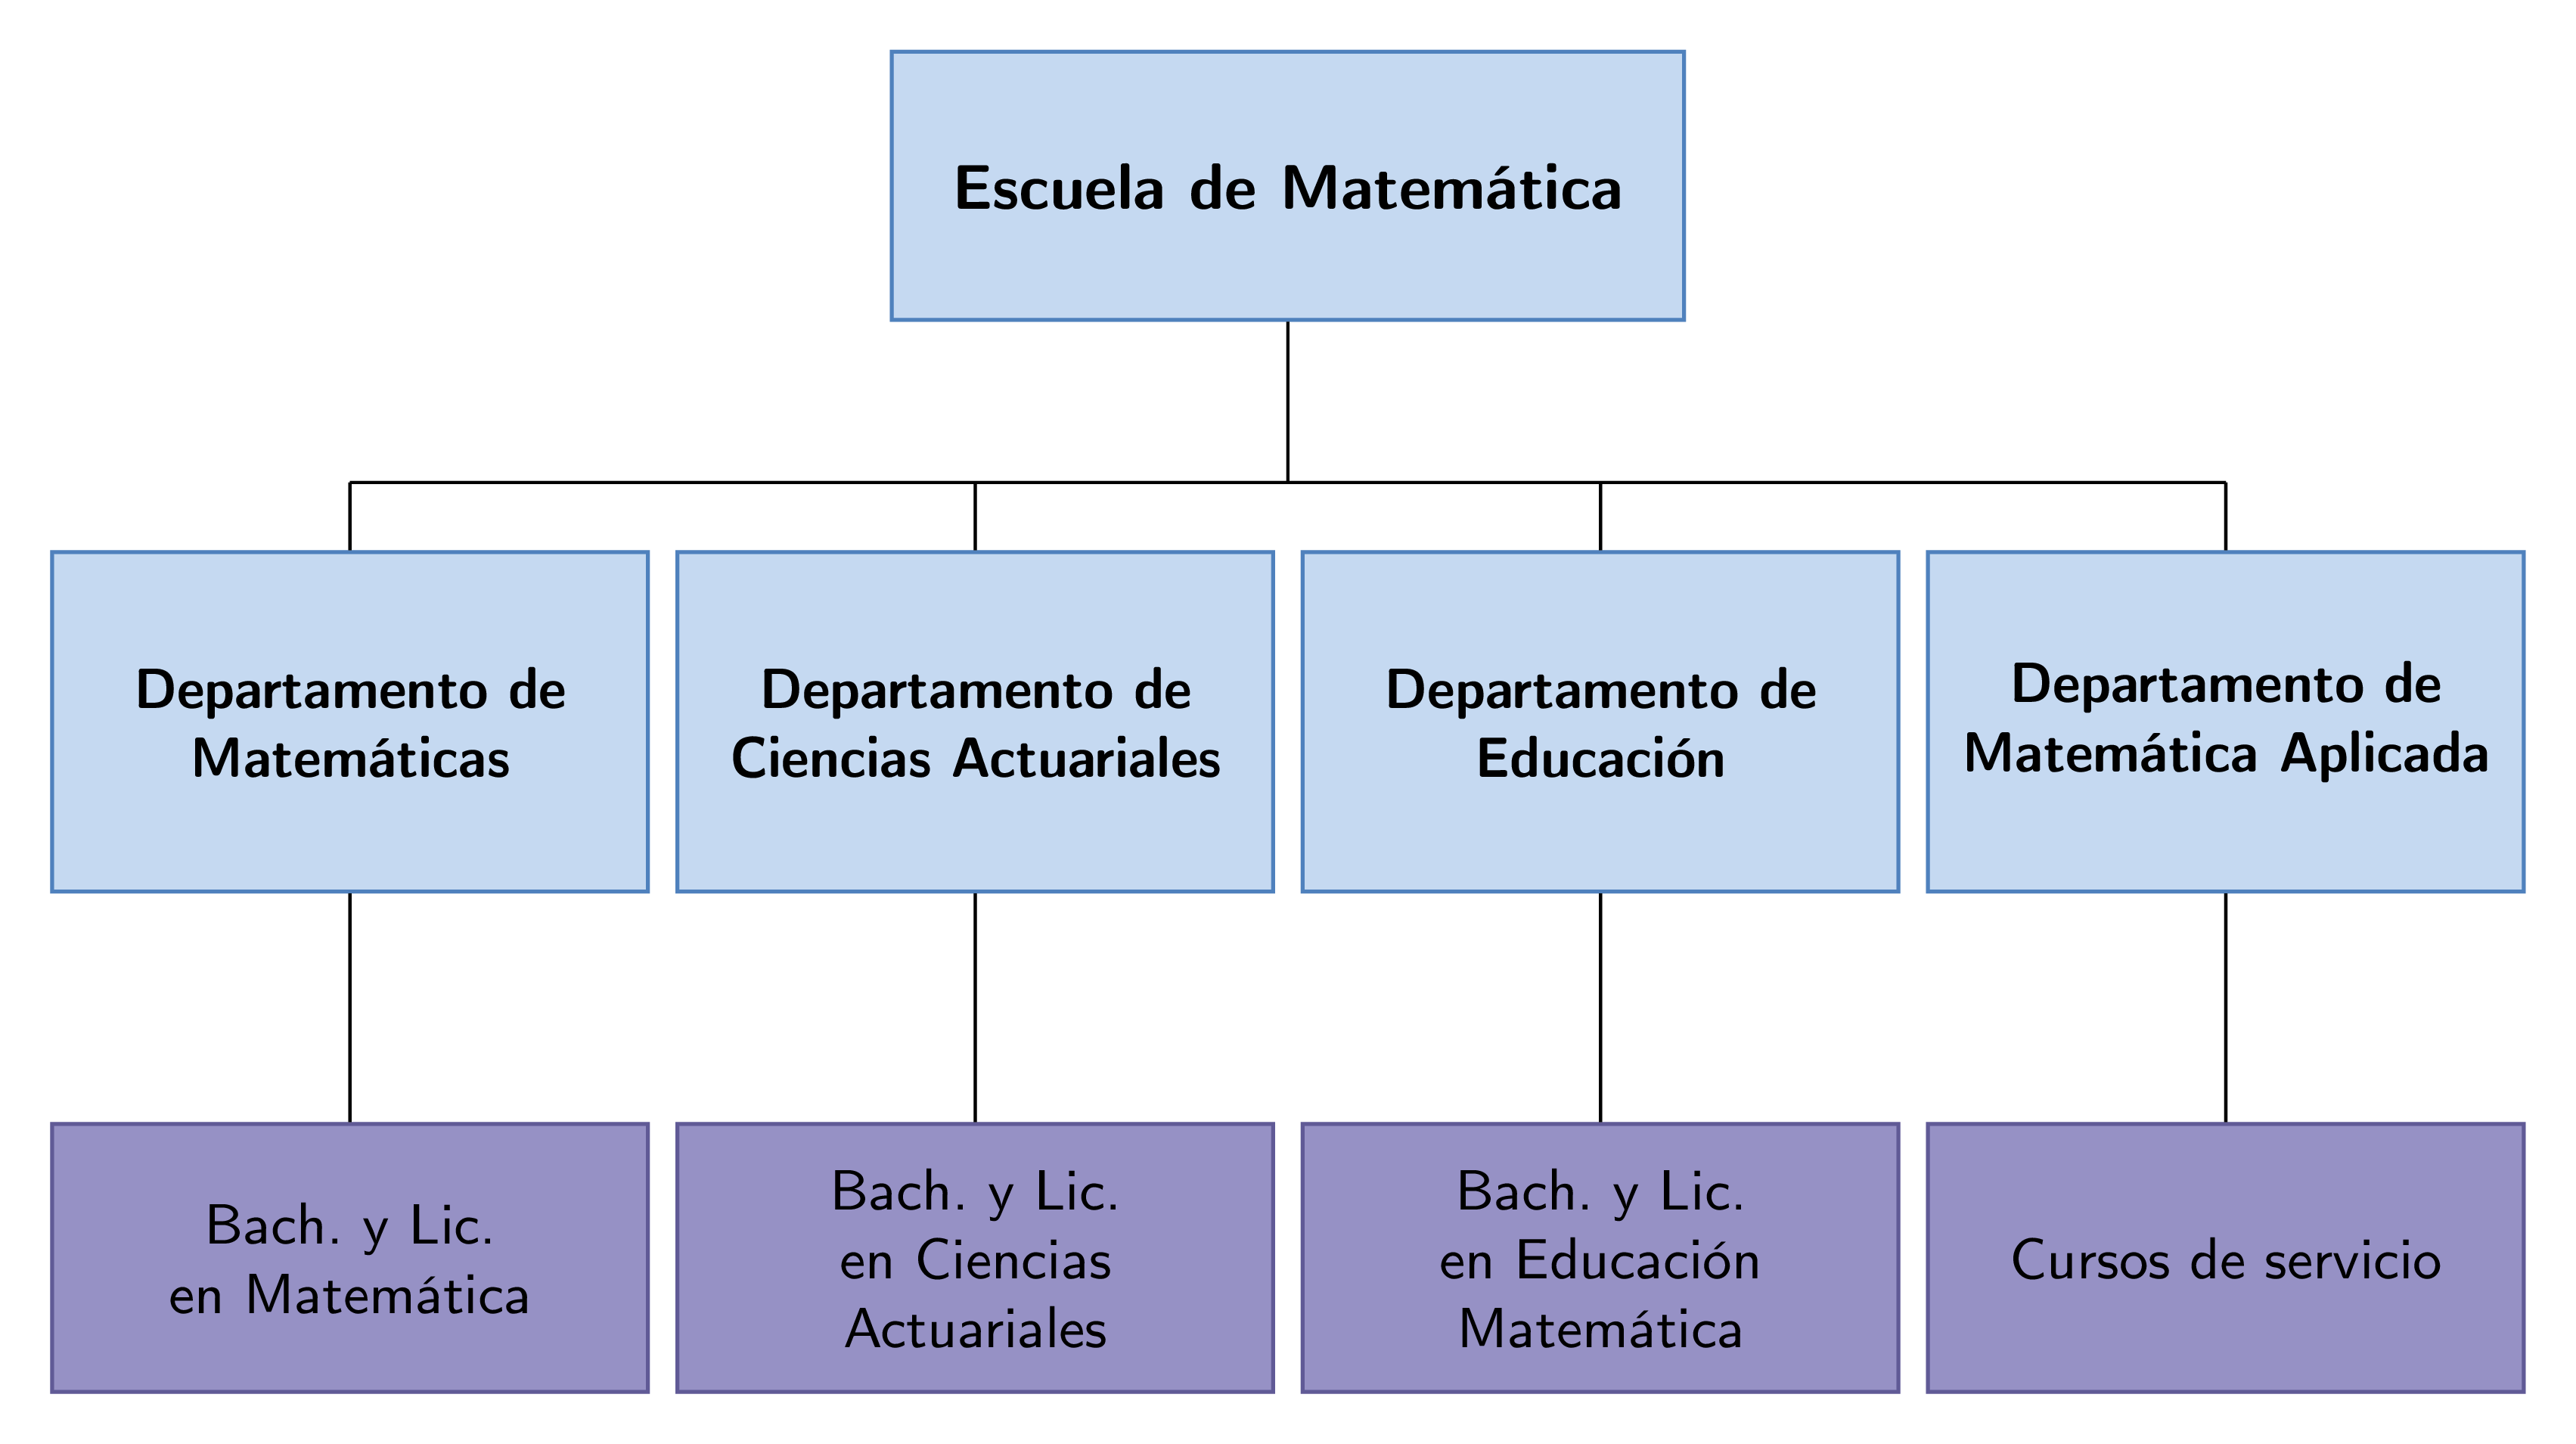
\includegraphics[width=0.5\linewidth]{dptos2.png}
    \caption{División por departamentos vigente en la Escuela de Matemática}
    \label{fig:dpto}
\end{figure}

\subsection{Cuerpo docente}
En la Tabla \ref{tab:docentes} se presenta el personal docente activo que ha impartido cursos en la carrera de Matemática desde el año 2010. Se clasifican por áreas de especialización, que corresponde a la especialización que tiene más cercanía a las áreas curriculares que se definieron con anterioridad. En la última columna de la tabla se especifica si el nombramiento de cada docente es en propiedad (P), becario (B), exbecario (E), o interinazgo (I).

% Please add the following required packages to your document preamble:
% \usepackage{longtable}
% Note: It may be necessary to compile the document several times to get a multi-page table to line up properly
\begin{longtable}[c]{|l|l|c|}
\caption{Lista de docentes en condición activa que han impartido cursos desde el 2010.}
\label{tab:docentes}\\
\hline
\rowcolor[HTML]{00C0F3}
Docente & Especialidad & Nombramiento \\ \hline
%
\endhead
%
Jennifer Acuña Larios & Análisis & P \\ \hline
Luis Acuña Valverde &  & P \\ \hline
Josué Ávila Artavia &  & E \\ \hline
Luis Barboza Chinchilla &  & P \\ \hline
Adrián Barquero Sánchez &  & P \\ \hline
Raúl Bolaños Guerrero &  & P \\ \hline
Ronald Bustamante Medina &  & P \\ \hline
Juan Gabriel Calvo Alpízar &  & P \\ \hline
Santiago Cambronero Villalobos &  & P \\ \hline
José David Campos Fernández &  & P \\ \hline
Daniel Campos Salas &  & P \\ \hline
Santiago Chaves Aguilar &  & E \\ \hline
Pedro Díaz Navarro &  & I \\ \hline
Christian Fonseca Mora &  & P \\ \hline
Álvaro Guevara Villalobos &  & P \\ \hline
Jorge Guier Acosta &  & P \\ \hline
Jonathan Gutiérrez Pavón &  & P \\ \hline
Alberto Hernández Alvarado &  & P \\ \hline
David Jiménez López &  & P \\ \hline
David Krumm Cabezas &  & I \\ \hline
Allan Lacy Mora &  & P \\ \hline
Jennifer Loría Sorio &  & E \\ \hline
Darío Mena Arias &  & P \\ \hline
Pedro Méndez Hernández &  & P \\ \hline
Carlos Montalto Cruz &  & P \\ \hline
Samaria Montenegro Guzmán &  & P \\ \hline
German Mora Sáenz &  & B \\ \hline
Adrián Naranjo Alvarado &  & B \\ \hline
Hugo Peña Gómez &  & I \\ \hline
Alexander Ramírez González &  & P \\ \hline
Oldemar Rodríguez Rojas &  & P \\ \hline
José Rosales Ortega &  & P \\ \hline
Adriana Sánchez Chavarría &  & P \\ \hline
Jesús Sánchez Guevara &  & P \\ \hline
Fabio Sánchez Peña &  & P \\ \hline
Esteban Segura Ugalde &  & P \\ \hline
Filánder Sequeira Chavarría &  & I \\ \hline
Maikol Solís Chacón &  & P \\ \hline
Javier Trejos Zelaya &  & P \\ \hline
William Ugalde Gómez &  & P \\ \hline
Roberto Ulloa Esquivel &  & E \\ \hline
Mario Villalobos Arias &  & P \\ \hline
Mark Villarino Bertran &  & P \\ \hline
Rafael Zamora Calero &  & P \\ \hline
Óscar Zamora Luna &  & E \\ \hline
Ronald Zúñiga Rojas &  & P \\ \hline
\end{longtable}


Con base en la información anterior, se detalla la cantidad de profesores disponibles (no exclusivos) por cada uno de los cursos que componen la malla curricular propuesta en la Tabla \ref{tab:cursos}. Es importante agregar que muchos docentes están simultáneamente disponibles en más de un curso, por lo que esta tabla representa un escenario optimista de la cantidad de recursos disponibles en la Escuela de Matemática para hacerle frente a la oferta académica. Cada curso se espera que sea impartido por docentes con doctorado. En el caso de tener maestría, se permitirá si el  curso es relacionado con el área de trabajo. %Por otro lado, la columna que indica el grado académico mínimo es definido con respecto a la complejidad de los contenidos y a la ubicación del curso en la malla curricular.


\begin{longtable}[c]{|l|p{7cm}|p{3.4cm}|p{2cm}|}
\caption{Número de personal docente por curso del nuevo plan de estudios, según especialidad}
\label{tab:cursos}\\
\hline
\rowcolor[HTML]{00C0F3}
Sigla & Curso & Área de especialidad & Número de docentes \\ \hline
%
\endhead
%
\MA{0151} & \gls{MA0151} & General &  \\ \hline
\MA{0152} & \gls{MA0152} & General &  \\ \hline
\MA{0251} & \gls{MA0251} & General &  \\ \hline
\MA{0252} & \gls{MA0252} & General &  \\ \hline
\MA{0261} & \gls{MA0261} & Álgebra &  \\ \hline
\MA{0341} & \gls{MA0341} & Numérico &  \\ \hline
\MA{0351} & \gls{MA0351} & Análisis &  \\ \hline
\MA{0361} & \gls{MA0361} & Álgebra &  \\ \hline
\MA{0451} & \gls{MA0451} & Análisis &  \\ \hline
\MA{0461} & \gls{MA0461} & Teoría de números &  \\ \hline
\MA{0471} & \gls{MA0471} & Análisis &  \\ \hline
\MA{0472} & \gls{MA0472} & Geometría &  \\ \hline
\MA{0515} & \gls{MA0515} & Análisis &  \\ \hline
\MA{0520} & \gls{MA0520} & Análisis/Estadística &  \\ \hline
\MA{0535} & \gls{MA0535} & Álgebra &  \\ \hline
\MA{0541} & \gls{MA0541} & Numérico &  \\ \hline
\MA{0615} & \gls{MA0615} & Análisis &  \\ \hline
\MA{0625} & \gls{MA0625} & Análisis &  \\ \hline
\MA{0635} & \gls{MA0635} & Álgebra &  \\ \hline
\MA{063X} & \gls{MA063X} & Topología &  \\ \hline
\MA{0702} & \gls{MA0702} & Análisis &  \\ \hline
\MA{0725} & \gls{MA0725} & Análisis &  \\ \hline
\MA{07xx} & \gls{MA07xx} & Geometría &  \\ \hline
\MA{-OPT} & \gls{OPT-Algebra} & Álgebra &  \\ \hline
\MA{-OPT} & \gls{OPT-Analisis} & Análisis &  \\ \hline
\MA{-OPT} & \gls{OPT-Aplicada} & Aplicada &  \\ \hline
\MA{-OPT} & \gls{OPT-Computacion cientifica} & Numérico &  \\ \hline
\MA{-OPT} & \gls{OPT-Discreta} & Discreta &  \\ \hline
\MA{-OPT} & \gls{OPT-Estadistica, Ciencia datos} & Estadística&  \\ \hline
\MA{-OPT} & \gls{OPT-Geometria} & Geometría &  \\ \hline
\MA{-OPT} & \gls{OPT-Logica} & Lógica &  \\ \hline
\MA{-OPT} & \gls{OPT-Topologia} & Topología &  \\ \hline
%\end{tabular}
\end{longtable}


\subsection{Plan de Transición}
Para estudiantes activos que ingresaron en el año 2025 o anteriores, se propone un plan de transición con base en el cohorte que corresponda, bajo el supuesto de que cada estudiante tiene el año correspondiente al cohorte completo al finalizar el año 2025. Los documentos completos se incluyen en el Anexo ??.

\subsubsection{Cohorte C7}
Se estima que este grupo tendrá XX estudiantes, quienes aprobaron MA0150 y MA0250, además de los cursos de generales de primer año. %A este grupo se le debe convalidar MA0251, MA0252 y permitir que MA0261 sea correquisito con los cursos del I26, como excepción por el plan de transición.

\begin{table}[h!]
\centering
\begin{tabular}{|l|l|}
\hline
\rowcolor[HTML]{00C0F3}
Cohorte C7 & Primer año completo del plan anterior \\ \hline
I28 & \begin{tabular}[c]{@{}l@{}}\textbf{Pura y Aplicada:}\\ SR-I Seminario de Realidad Nacional I (2)\\ MA0361 Álgebra Lineal I (4)\\ EG- Curso de Arte (2)\\ MA0351 Cálculo en Varias Variables (4)\\ MA0341 Matemática Computacional (4)\end{tabular} \\ \hline
II28 & \begin{tabular}[c]{@{}l@{}}\textbf{Pura y Aplicada:} igual que el ciclo IV del plan 03\end{tabular} \\ \hline
I29 & \begin{tabular}[c]{@{}l@{}}\textbf{Pura y Aplicada:} igual que el ciclo V del plan 03\end{tabular} \\ \hline
II29 & \begin{tabular}[c]{@{}l@{}}\textbf{Pura y Aplicada:} igual que el ciclo VI del plan 03\end{tabular} \\ \hline
I30 & \begin{tabular}[c]{@{}l@{}}\textbf{Pura y Aplicada:} igual que el ciclo VII del plan 03\end{tabular} \\ \hline
II30 & \begin{tabular}[c]{@{}l@{}}\textbf{Pura y Aplicada:} igual que el ciclo VIII del plan 03\end{tabular} \\ \hline
\end{tabular}
\end{table}

% \begin{table}[h!]
% \centering
% \begin{tabular}{|c|l|}
% \hline
% \rowcolor[HTML]{00C0F3}
% Cohorte C5 & Primer año completo del plan anterior \\ \hline
% I26 & \begin{tabular}[c]{@{}l@{}}MA0261 \gls{MA0261} (3)\\ MA0341 \gls{MA0341} (4)\\ MA0351 \gls{MA0351} (4)\\ Artística (2)\end{tabular} \\ \hline
% II26 & \begin{tabular}[c]{@{}l@{}}MA0361 \gls{MA0361} (4)\\ MA0451 \gls{MA0451} (4)\\ MA0461 \gls{MA0461} (4)\\ MA0471 \gls{MA0471} (4)\\ Seminario de Realidad Nacional I (2)\end{tabular} \\ \hline
% I27 & Igual que Ciclo V - Plan 26 \\ \hline
% II 27 & Igual que Ciclo VI - Plan 26 \\ \hline
% I 28 & Igual que Ciclo VII - Plan 26 \\ \hline
% II 28 & Igual que Ciclo VIII - Plan 26 \\ \hline
% \end{tabular}
% \end{table}

\subsubsection{Cohorte C6}
Se estima que este grupo tendrá XX estudiantes, quienes aprobaron MA0150, MA0250, MA0350, MA0360, MA0370, MA0450 y MA0460. %A este grupo se le debe convalidar MA0252, MA0351, MA0341, y permitir que MA0461 y MA0535 sean correquisitos, como excepción por el plan de transición.

\begin{table}[h!]
\centering
\begin{tabular}{|l|l|}
\hline
\rowcolor[HTML]{00C0F3}
Cohorte C6 & Dos primeros años completos del plan anterior \\ \hline
I28 & \begin{tabular}[c]{@{}l@{}}\textbf{Pura:}\\ MA0561 Álgebra Abstracta I (4)\\ MA0471 Introducción a la Geometría Diferencial (3)\\ MA0515 Ecuaciones Diferenciales Ordinarias (4)\\ Optativa de otra disciplina (3)\\ \textbf{Aplicada:}\\ MA0635 Topología General (4)\\ MA0515 Ecuaciones Diferenciales Ordinarias (4)\\ Optativa específica de matemática (4)\\ Optativa de otra disciplina (4)\end{tabular} \\ \hline
II28 & \begin{tabular}[c]{@{}l@{}}\textbf{Pura:} igual que el ciclo VI del plan 03\\ \textbf{Aplicada:}\\ CA0204 Herramientas de Ciencia de Datos I (4)\\ MA0647 Modelación Matemática (4)\\ CA0721 Probabilidad (4)\\ MA0641 Análisis Numérico I (4)\end{tabular} \\ \hline
I29 & \begin{tabular}[c]{@{}l@{}}\textbf{Pura:} igual que el ciclo VII del plan 03\\ \textbf{Aplicada:}\\ CA0303 Estadística Actuarial I (4)\\ MA0702 Análisis Complejo (4)\\ MA0705 Análisis Real I (4)\\ MA0780 Comunicación en las Ciencias (2)\\ MA0701 Seminario (0)\end{tabular} \\ \hline
II29 & \begin{tabular}[c]{@{}l@{}}\textbf{Pura:} igual que el ciclo VIII del plan 03\\ \textbf{Aplicada:}\\ CA0411 Análisis de Datos I (4)\\ Optativa específica de matemática (4)\\ Optativa específica de matemática (4)\\ MA0781 Pasantía (4)\end{tabular} \\ \hline
\end{tabular}
\end{table}

% \begin{table}[h!]
% \centering
% \begin{tabular}{|l|l|}
% \hline
% \rowcolor[HTML]{00C0F3}
% Cohorte C4 & Segundo año completo del plan anterior) \\ \hline
% I26 & \begin{tabular}[c]{@{}l@{}} {MA0561} (4), MA0515 (4), MA0471 (3), optativa otra disciplina\\ Aplicada: CA0721, CA0203, MA0515, optativa \\
% **MA0461 \gls{MA0461} (4)\\ MA0520 \gls{MA0520} (4)\\ MA0535 \gls{MA0535} (4)\\ MA0541 \gls{MA0541} (4)\\ Seminario de Realidad Nacional II (2)\end{tabular} \\ \hline
% II26 & Igual que Ciclo VI - Plan 26\\ Aplicada: \\ \hline
% I27 & Igual que Ciclo VII - Plan 26\\ Aplicada: \\ \hline
% II 27 & Igual que Ciclo VIII - Plan 26\\ Aplicada: \\ \hline
% \end{tabular}
% \end{table}

\subsubsection{Cohorte C5}
Quienes tengan tres años completos del plan 02, deben finalizar dicho plan. Para ello deben cursar MA0702, MA0704, MA0870, una optativa de otra disciplina y tres optativas de Matemática. Posteriormente, podrán continuar en la licenciatura del plan 03.

\subsubsection{Excepciones}
Cada estudiante que no haya cumplido sus ciclos de estudio de acuerdo con el plan de estudios anterior, no contemplados en los incisos anteriores, o aquellos de planes previos, deberá de utilizar la tabla de convalidaciones para trasladarse hacia la malla del nuevo plan de estudios, y deberá cursar los cursos no convalidables hasta cumplir con todos los requisitos del plan 2028. 

\subsubsection{Convalidaciones}

Se plantea considerar convalidaciones para casos particulares que no cumplen con un cohorte específico; ver Tabla \ref{tab:conv}. De esta forma, se deberán trasladar al Plan 03 que inicia en el 2028, realizando las convalidaciones que correspondan, y deberán cursar aquellos cursos no convalidables hasta cumplir con todos los requisitos del plan 2028.

\begin{table}[h!]
\centering
\caption{Convalidaciones para la transición de plan de estudios}
\label{tab:conv}
\begin{tabular}{|p{7.25cm}|p{7.25cm}|}
\rowcolor[HTML]{00C0F3}
\hline
Sigla y curso aprobado & Sigla y curso por convalidar \\ \hline
MA0150 Principios de Matemática & MA0252 Introducción a las Demostraciones \\ \hline
MA0250 Cálculo en una Variable I & MA0251 Cálculo en una Variable \\ \hline
MA0350 Cálculo en una Variable II & MA0451 Principios de Análisis I \\ \hline
MA0360 Álgebra Lineal I & MA0361 Álgebra Lineal I \\ \hline
MA0370 Principios de Geometría & MA0496 Teoría de Números u Optativa Específica de Matemática \\ \hline
MA0450 Cálculo en Varias Variables & MA0551 Principios de Análisis II \\ \hline
MA0455 Ecuaciones Diferenciales Ordinarias & MA0515 Ecuaciones Diferenciales Ordinarias \\ \hline
MA0460 Álgebra Lineal II & MA0461 Álgebra Lineal II \\ \hline
MA0505 Análisis I & MA0705 Análisis Real I \\ \hline
MA0561 Grupos y Anillos & MA0561 Álgebra Abstracta I \\ \hline
MA0605 Análisis II & MA0725 Análisis Real II \\ \hline
MA0660 Teoría de Galois & MA0661 Álgebra Abstracta II \\ \hline
MA0702 Variable Compleja I & MA0702 Análisis Complejo \\ \hline
MA0704 Topología General I & MA0635 Topología General \\ \hline
MA0870 Geometría Diferencial & MA0471 Introducción a la Geometría Diferencial \\ \hline
OPT- Bloque de Optativos Específicos de Matemáticas & Optativa Específica de Matemática \\ \hline
Cursos de Licenciatura & Optativa Específica de Matemática \\ \hline
\end{tabular}
\end{table}

\subsection{Proyección de carga académica para el plan de transición}

Según el plan descrito en la sección anterior, se presenta la proyección de carga académica necesaria para suplir la demanda de los años de transición (2028, 2029, 2030). Esto bajo el supuesto de recibir el máximo de 26 estudiantes por año más doce estudiantes por traslado, ofertando dos grupos? por curso en primer año.

\begin{longtable}[c]{|p{0.7cm}|p{1.6cm}|p{6.4cm}|p{1.5cm}|p{1.2cm}|p{1.4cm}|}
\caption{Proyección de carga académica para el plan de transición, año 2028}
\label{tab:carga2028}\\
\hline
\rowcolor[HTML]{00C0F3}
Ciclo & Cohorte & Curso & Créditos & Grupos & Jornada \\ \hline
\endhead
%
I & C8P C8A & MA0151 Fundamentos de Álgebra, Trigonometría y Geometría Analítica & 3 & \textbf{2} & 0.375 \\ \hline
I & C8P C8A & MA0152 Matemática Exploratoria & 3 & \textbf{2} & 0.375 \\ \hline
I & C7P C7A & MA0341 Matemática Computacional & 4 & 1 & 0.375 \\ \hline
I & C7P C7A & MA0351 Cálculo en Varias Variables & 4 & 1 & 0.375 \\ \hline
I & C7P C7A & MA0361 Álgebra Lineal I & 4 & 1 & 0.375 \\ \hline
I & C6P & MA0471 Introducción a la Geometría Diferencial & 3 & 1 & 0.375 \\ \hline
I & C6P C6A & MA0515 Ecuaciones Diferenciales Ordinarias & 4 & 1 & 0.375 \\ \hline
I & C6P & MA0561 Álgebra Abstracta I & 4 & 1 & 0.375 \\ \hline
I & C6A & MA0635 Topología General & 4 & 1 & 0.375 \\ \hline
I & C5 & MA0702 Variable Compleja I & 5 & 1 & 0.375 \\ \hline
I & C5 & MA0704 Topología General I & 5 & 1 & 0.000 \\ \hline
I & C5 C6A& OPT- Bloque de Optativos Específicos de Matemáticas & 5 & 1 & 0.375 \\ \hline
%I & C6A & OPT- Optativa Específica de Matemática & 4 & 1 & 0.375 \\ \hline
 &  &  & Subtotal I Ciclo & 14 & 3.575 \\ \hline
II & C6A C7A & CA0204 Herramientas de Ciencia de Datos I & 4 & 1 & 0.375 \\ \hline
II & C6A C7A & CA0721 Probabilidad & 4 & 1 & 0.375 \\ \hline
II & C8P C8A & LM3039 Inglés para Estadística I & 3 & 1 & 0.250 \\ \hline
II & C8P C8A & MA0251 Cálculo en una Variable & 3 & 1 & 0.375 \\ \hline
II & C8P C8A & MA0252 Introducción a las Demostraciones & 4 & 1 & 0.375 \\ \hline
II & C7P C7A & MA0451 Principios de Análisis I & 4 & 1 & 0.375 \\ \hline
II & C7P C7A & MA0461 Álgebra Lineal II & 4 & 1 & 0.375 \\ \hline
II & C7P & MA0471 Introducción a la Geometría Diferencial & 3 & 1 & 0.375 \\ \hline
II & C7P & MA0496 Teoría de Números & 3 & 1 & 0.375 \\ \hline
II & C6P & MA0635 Topología General & 4 & 1 & 0.375 \\ \hline
II & C6P C6A & MA0641 Análisis Numérico I & 4 & 1 & 0.375 \\ \hline
II & C6A & MA0647 Modelación Matemática & 4 & 1 & 0.375 \\ \hline
II & C6P & MA0661 Álgebra Abstracta II & 4 & 1 & 0.375 \\ \hline
II & C5 & MA0870 Geometría Diferencial & 5 & 1 & 0.375 \\ \hline
II & C5 & OPT- Bloque de Optativos Específicos de Matemáticas & 5 & 1 & 0.375 \\ \hline
II & C5 & OPT- Bloque de Optativos Específicos de Matemáticas & 5 & 1 & 0.375 \\ \hline
 &  &  & Subtotal II Ciclo & 16 & 5.875 \\ \hline
 &  &  & Total del año & 29 & 9.450 \\ \hline
\end{longtable}

\begin{longtable}[c]{|p{0.8cm}|p{1.8cm}|p{6.8cm}|p{1.5cm}|p{1.3cm}|p{1.5cm}|}
\caption{Proyección de carga académica para el plan de transición, año 2029}
\label{tab:carga2029}\\
\hline
\rowcolor[HTML]{00C0F3}
Ciclo & Cohorte & Curso & Créditos & Grupos & Jornada \\ \hline
\endhead
%
I & C6A C7A & CA0303 Estadística Actuarial I & 4 & 1 & 0.375 \\ \hline
I & C8P C8A & LM3040 Inglés para Estadística II & 3 & 1 & 0.250 \\ \hline
I & C9P C9A & MA0151 Fundamentos de Álgebra, Trigonometría y Geometría Analítica & 3 & 1 & 0.375 \\ \hline
I & C9P C9A & MA0152 Matemática Exploratoria & 3 & 1 & 0.375 \\ \hline
I & C8P C8A & MA0341 Matemática Computacional & 4 & 1 & 0.375 \\ \hline
I & C8P C8A & MA0351 Cálculo en Varias Variables & 4 & 1 & 0.375 \\ \hline
I & C8P C8A & MA0361 Álgebra Lineal I & 4 & 1 & 0.375 \\ \hline
I & C7P C7A & MA0515 Ecuaciones Diferenciales Ordinarias & 4 & 1 & 0.375 \\ \hline
I & C7P C7A & MA0551 Principios de Análisis II & 4 & 1 & 0.375 \\ \hline
I & C7P & MA0561 Álgebra Abstracta I & 4 & 1 & 0.375 \\ \hline
I & C6P C6A & MA0701 Seminario & 0 & 1 & 0.000 \\ \hline
I & C6P C6A & MA0702 Análisis Complejo & 4 & 1 & 0.375 \\ \hline
I & C6P C6A & MA0705 Análisis Real I & 4 & 1 & 0.375 \\ \hline
I & C6P C6A & MA0780 Comunicación en las Ciencias & 2 & 1 & 0.375 \\ \hline
I & C6P & OPT- Optativa Específica de Matemática & 4 & 1 & 0.375 \\ \hline
 &  &  & Subtotal I Ciclo & 15 & 5.4375 \\ \hline
II & C8A & CA0204 Herramientas de Ciencia de Datos I & 4 & 1 & 0.375 \\ \hline
II & C6A & CA0411 Análisis de Datos I & 4 & 1 & 0.375 \\ \hline
II & C8A & CA0721 Probabilidad & 4 & 1 & 0.375 \\ \hline
II & C9P C9A & LM3039 Inglés para Estadística I & 3 & 1 & 0.1875 \\ \hline
II & C9P C9A & MA0251 Cálculo en una Variable & 3 & 1 & 0.375 \\ \hline
II & C9P C9A & MA0252 Introducción a las Demostraciones & 4 & 1 & 0.375 \\ \hline
II & C8P C8A & MA0451 Principios de Análisis I & 4 & 1 & 0.375 \\ \hline
II & C8P C8A & MA0461 Álgebra Lineal II & 4 & 1 & 0.375 \\ \hline
II & C8P & MA0471 Introducción a la Geometría Diferencial & 3 & 1 & 0.375 \\ \hline
II & C8P & MA0496 Teoría de Números & 3 & 1 & 0.375 \\ \hline
II & C7P C7A & MA0635 Topología General & 4 & 1 & 0.375 \\ \hline
II & C7P C7A & MA0641 Análisis Numérico I & 4 & 1 & 0.375 \\ \hline
II & C7A & MA0647 Modelación Matemática & 4 & 1 & 0.375 \\ \hline
II & C7P & MA0661 Álgebra Abstracta II & 4 & 1 & 0.375 \\ \hline
II & C6P C6A & MA0781 Pasantía & 4 & 1 & 0.000 \\ \hline
II & C6P C6A & OPT- Optativa Específica de Matemática & 4 & 1 & 0.375 \\ \hline
II & C6P C6A & OPT- Optativa Específica de Matemática & 4 & 1 & 0.375 \\ \hline
II & C6P & OPT- Optativa Específica de Matemática & 4 & 1 & 0.375 \\ \hline
 &  &  & Subtotal II Ciclo & 18 & x.5625 \\ \hline
 &  &  & Total del año & 33 & xx \\ \hline
\end{longtable}

% anchos de columna: Ciclo | Cohorte | Curso | Créditos | Grupos | Jornada
\begin{longtable}[c]{|p{0.8cm}|p{1.8cm}|p{6.8cm}|p{1.5cm}|p{1.3cm}|p{1.5cm}|}
\caption{Proyección de carga académica para el plan de transición, año 2030}
\label{tab:carga2030}\\
\hline
\rowcolor[HTML]{00C0F3}
Ciclo & Cohorte & Curso & Créditos & Grupos & Jornada \\ \hline
\endhead
%
I & C8A & CA0303 Estadística Actuarial I & 4 & 1 & 0.375 \\ \hline
I & C7A & CA0411 Análisis de Datos I & 4 & 1 & 0.375 \\ \hline
I & C9P C9A & LM3040 Inglés para Estadística II & 3 & 1 & 0.1875 \\ \hline
I & C10P C10A & MA0151 Fundamentos de Álgebra, Trigonometría y Geometría Analítica & 3 & 1 & 0.375 \\ \hline
I & C10P C10A & MA0152 Matemática Exploratoria & 3 & 1 & 0.375 \\ \hline
I & C9P C9A & MA0341 Matemática Computacional & 4 & 1 & 0.375 \\ \hline
I & C9P C9A & MA0351 Cálculo en Varias Variables & 4 & 1 & 0.375 \\ \hline
I & C9P C9A & MA0361 Álgebra Lineal I & 4 & 1 & 0.375 \\ \hline
I & C8P C8A & MA0515 Ecuaciones Diferenciales Ordinarias & 4 & 1 & 0.375 \\ \hline
I & C8P C8A & MA0551 Principios de Análisis II & 4 & 1 & 0.375 \\ \hline
I & C8P & MA0561 Álgebra Abstracta I & 4 & 1 & 0.375 \\ \hline
I & C7P C7A & MA0701 Seminario & 0 & 1 & 0.375 \\ \hline
I & C7P C7A & MA0702 Análisis Complejo & 4 & 1 & 0.375 \\ \hline
I & C7P C7A & MA0705 Análisis Real I & 4 & 1 & 0.375 \\ \hline
I & C7P C7A & MA0780 Comunicación en las Ciencias & 2 & 1 & 0.375 \\ \hline
I & C7P & OPT- Optativa Específica de Matemática & 4 & 1 & 0.375 \\ \hline
 &  &  & Subtotal I Ciclo & 16 & 5.8125 \\ \hline
II & C9A & CA0204 Herramientas de Ciencia de Datos I & 4 & 1 & 0.375 \\ \hline
II & C9A & CA0721 Probabilidad & 4 & 1 & 0.375 \\ \hline
II & C10P C10A & LM3039 Inglés para Estadística I & 3 & 1 & 0.1875 \\ \hline
II & C10P C10A & MA0251 Cálculo en una Variable & 3 & 1 & 0.375 \\ \hline
II & C10P C10A & MA0252 Introducción a las Demostraciones & 4 & 1 & 0.375 \\ \hline
II & C9P C9A & MA0451 Principios de Análisis I & 4 & 1 & 0.375 \\ \hline
II & C9P C9A & MA0461 Álgebra Lineal II & 4 & 1 & 0.375 \\ \hline
II & C9P & MA0471 Introducción a la Geometría Diferencial & 3 & 1 & 0.375 \\ \hline
II & C9P & MA0496 Teoría de Números & 3 & 1 & 0.375 \\ \hline
II & C8P C8A & MA0635 Topología General & 4 & 1 & 0.375 \\ \hline
II & C8P C8A & MA0641 Análisis Numérico I & 4 & 1 & 0.375 \\ \hline
II & C8A & MA0647 Modelación Matemática & 4 & 1 & 0.375 \\ \hline
II & C8P & MA0661 Álgebra Abstracta II & 4 & 1 & 0.375 \\ \hline
II & C7P C7A & MA0781 Pasantía & 4 & 1 & 0.375 \\ \hline
II & C7P C7A & OPT- Optativa Específica de Matemática & 4 & 1 & 0.375 \\ \hline
II & C7P C7A & OPT- Optativa Específica de Matemática & 4 & 1 & 0.375 \\ \hline
II & C7P C7A & OPT- Optativa Específica de Matemática & 4 & 1 & 0.375 \\ \hline
 &  &  & Subtotal II Ciclo & 17 & 6.1875 \\ \hline
 &  &  & Total del año & 33 & 12 \\ \hline
\end{longtable}

% anchos de columna: Ciclo | Cohorte | Curso | Créditos | Grupos | Jornada
\begin{longtable}[c]{|p{0.8cm}|p{1.8cm}|p{6.8cm}|p{1.5cm}|p{1.3cm}|p{1.5cm}|}
\caption{Proyección de carga académica para el plan de transición, año 2031}
\label{tab:carga2031}\\
\hline
\rowcolor[HTML]{00C0F3}
Ciclo & Cohorte & Curso & Créditos & Grupos & Jornada \\ \hline
\endhead
%
I & C9A & CA0303 Estadística Actuarial I & 4 & 1 & 0.375 \\ \hline
I & C8A & CA0411 Análisis de Datos I & 4 & 1 & 0.375 \\ \hline
I & C10P C10A & LM3040 Inglés para Estadística II & 3 & 1 & 0.1875 \\ \hline
I & C11P C11A & MA0151 Fundamentos de Álgebra, Trigonometría y Geometría Analítica & 3 & 1 & 0.375 \\ \hline
I & C11P C11A & MA0152 Matemática Exploratoria & 3 & 1 & 0.375 \\ \hline
I & C10P C10A & MA0341 Matemática Computacional & 4 & 1 & 0.375 \\ \hline
I & C10P C10A & MA0351 Cálculo en Varias Variables & 4 & 1 & 0.375 \\ \hline
I & C10P C10A & MA0361 Álgebra Lineal I & 4 & 1 & 0.375 \\ \hline
I & C9P C9A & MA0515 Ecuaciones Diferenciales Ordinarias & 4 & 1 & 0.375 \\ \hline
I & C9P C9A & MA0551 Principios de Análisis II & 4 & 1 & 0.375 \\ \hline
I & C9P & MA0561 Álgebra Abstracta I & 4 & 1 & 0.375 \\ \hline
I & C8P C8A & MA0701 Seminario & 0 & 1 & 0.375 \\ \hline
I & C8P C8A & MA0702 Análisis Complejo & 4 & 1 & 0.375 \\ \hline
I & C8P C8A & MA0705 Análisis Real I & 4 & 1 & 0.375 \\ \hline
I & C8P C8A & MA0780 Comunicación en las Ciencias & 2 & 1 & 0.375 \\ \hline
I & C8P & OPT- Optativa Específica de Matemática & 4 & 1 & 0.375 \\ \hline
 &  &  & Subtotal I Ciclo & 16 & 5.8125 \\ \hline
II & C10A & CA0204 Herramientas de Ciencia de Datos I & 4 & 1 & 0.375 \\ \hline
II & C10A & CA0721 Probabilidad & 4 & 1 & 0.375 \\ \hline
II & C11P C11A & LM3039 Inglés para Estadística I & 3 & 1 & 0.1875 \\ \hline
II & C11P C11A & MA0251 Cálculo en una Variable & 3 & 1 & 0.375 \\ \hline
II & C11P C11A & MA0252 Introducción a las Demostraciones & 4 & 1 & 0.375 \\ \hline
II & C10P C10A & MA0451 Principios de Análisis I & 4 & 1 & 0.375 \\ \hline
II & C10P C10A & MA0461 Álgebra Lineal II & 4 & 1 & 0.375 \\ \hline
II & C10P & MA0471 Introducción a la Geometría Diferencial & 3 & 1 & 0.375 \\ \hline
II & C10P & MA0496 Teoría de Números & 3 & 1 & 0.375 \\ \hline
II & C9P C9A & MA0635 Topología General & 4 & 1 & 0.375 \\ \hline
II & C9P C9A & MA0641 Análisis Numérico I & 4 & 1 & 0.375 \\ \hline
II & C9A & MA0647 Modelación Matemática & 4 & 1 & 0.375 \\ \hline
II & C9P & MA0661 Álgebra Abstracta II & 4 & 1 & 0.375 \\ \hline
II & C8P C8A & MA0781 Pasantía & 4 & 1 & 0.375 \\ \hline
II & C8P C8A & OPT- Optativa Específica de Matemática & 4 & 1 & 0.375 \\ \hline
II & C8P C8A & OPT- Optativa Específica de Matemática & 4 & 1 & 0.375 \\ \hline
II & C8P C8A & OPT- Optativa Específica de Matemática & 4 & 1 & 0.375 \\ \hline
 &  &  & Subtotal II Ciclo & 17 & 6.1875 \\ \hline
 &  &  & Total del año & 33 & 12 \\ \hline
\end{longtable}

% anchos de columna: Año | Grupos I | Jornada I | Grupos II | Jornada II | Total grupos | Jornada total
\begin{longtable}[c]{|p{1.2cm}|p{2cm}|p{2.1cm}|p{2cm}|p{2.1cm}|p{1.9cm}|p{2cm}|}
\caption{Resumen de la proyección de carga académica, 2028--2031 [NO ESTA ACTUALIZADA]}
\label{tab:cargaresumen}\\
\hline
\rowcolor[HTML]{00C0F3}
Año & Grupos I Ciclo & Jornada I Ciclo & Grupos II Ciclo & Jornada II Ciclo & Total grupos & Jornada total \\ \hline
\endhead
%
2028 & 13 & 4.875 & 16 & 5.8125 & 29 & 10.6875 \\ \hline
2029 & 15 & 5.4375 & 18 & 6.5625 & 33 & 12 \\ \hline
2030 & 16 & 5.8125 & 17 & 6.1875 & 33 & 12 \\ \hline
2031 & 16 & 5.8125 & 17 & 6.1875 & 33 & 12 \\ \hline
%Total &  &  &  &  & 128 & 46.6875 \\ \hline
\end{longtable}


\section{Seguimiento y Evaluación}

En esta sección se plantea la estrategia de evaluación de la carrera y el plan de desarrollo docente que la Escuela de Matemática podría implementar para capacitar al cuerpo docente ante las nuevas exigencias académicas de la malla propuesta.

\subsection{Momentos y estrategias de evaluación de la carrera}

La puesta en marcha de esta propuesta estará a cargo de la persona directora del Departamento de Matemática, en conjunto con la comisión que elaboró esta propuesta, quienes supervisarán la implementación completa del proceso de transición y la asignación y ejecución de carga presupuestaria tal y como se detalla en la Sección 5.1. Asimismo, será el Departamento de Matemática el encargado de ejecutar las estrategias de desarrollo docente que se explican en la siguiente sección, preferiblemente a través de la conformación de una comisión con ese objetivo en particular. 
Por otro lado, se recomienda que el Departamento nombre una comisión encargada de la evaluación de la malla curricular propuesta para que tenga listo un diagnóstico del perfil de salida y de la malla vigente a lo sumo cinco años después de que el plan se haya incorporado de manera completa en la población estudiantil. Se recomienda que los mismos miembros que conformaron la elaboración de este documento participen en esa comisión de evaluación.

\subsection{Desarrollo docente}

\subsection{Presupuesto}



\chapter{Anexos}


\chapter{Anexos}


\section{Caracterización profesional}
\label{sec:CaractProf}

La caracterización profesional se aborda desde dos análisis complementarios, el primero de estos corresponde al análisis de las prácticas profesionales, y, el segundo, a la definición profesional. Para esto se considera cada análisis estructural de la actividad realizado con los docentes, según identidad matemática, y también una consulta con otros especialistas. 


\subsection{Análisis de las prácticas profesionales}


Este apartado se lleva a cabo por medio de categorías que se establecen para valorar las prácticas que, actualmente, trabajan los profesionales en Matemática, desde aquellas prácticas que han dejado de ser prioridades hasta las que son oportunidades para el matemático del futuro. Al respecto, se establecen las categorías de prácticas emergentes, dominantes y decadentes, con sus respectivas categorías y una forma de comprender el motivo por el cual han sido valoradas de esa forma.

\subsubsection{Prácticas emergentes}

\subsubsection*{Investigación fuera de la academia en disciplinas afines}


En el mundo, y, particularmente, en nuestro país, es notorio el crecimiento de la demanda de matemáticos en disciplinas tan variadas como las finanzas, la banca, la economía, la estadística. El trabajo interdisciplinario y las habilidades de liderazgo, para la conformación de equipos interdisciplinarios, se hacen cada vez más importantes e imprescindibles. 

El matemático de hoy en día debe estar en contacto permanente con los últimos acontecimientos científicos, no solo de la matemática propiamente, sino también de otras disciplinas afines. Debe saber entender y hacerse entender por otros profesionales, debe tener la empatía necesaria para interactuar, y dar respuestas satisfactorias a los requerimientos de otras disciplinas.

\subsubsection*{Análisis de datos}

La ciencia de los datos es aplicable, en términos generales, a diversas áreas (reconocimiento de imágenes, agrupamiento de datos, aprendizaje no supervisado, etc.). En resumen, la ciencia de
los datos está de moda. Las labores relacionadas con el manejo de datos a gran escala, ha hecho que el mercado, para los profesionales en áreas afines a la matemática, se expanda considerablemente. Esto, a su vez, ha provocado no solo una revalorización del matemático a nivel profesional, sino que, además, ha impactado la forma en que se hace mucha de la investigación académica, más de la mano del manejo e interpretación de datos. 

\subsubsection*{Experimentación científica cada vez más apoyada en la tecnología}

Los avances tecnológicos se han desencadenado de una manera impactante en las últimas décadas. Esto, sin duda, ha afectado de manera muy positiva el desarrollo de la investigación en matemática. Por citar ejemplos, la simulación de fenómenos naturales, que tiempo atrás se realizaba más de la mano de simulaciones mecánicas o mediante la observación directa, hoy en día es posible realizarla de manera más versátil mediante el uso de la tecnología. Al estudiar fenómenos financieros o económicos, o, en general, fenómenos de comportamiento social, las simulaciones estocásticas son una herramienta que, si bien han existido por décadas, cada vez están más a la mano y de manera más natural. El impacto de estos recursos para la investigación es innegable. 

\subsubsection{Prácticas dominantes}

\subsubsection*{Investigación académica}

La investigación académica, tanto teórica como aplicada, ha estado presente como una práctica profesional en matemática, posiblemente desde la antigüedad. Esta es una práctica que definitivamente no va a pasar de moda. El matemático es posiblemente uno de los científicos al que se le facilita más la investigación, sobre todo si esta es de carácter teórico, debido a que no requiere de realización de grandes experimentos en laboratorios sofisticados. Muchos grandes avances se pueden realizar solo con disciplina, lápiz y papel. 


\subsubsection*{Docencia Universitaria }


Es muy difícil desligar a un matemático de la Docencia Universitaria. Si bien, algunas prácticas emergentes han provocado que el sector productivo absorba ciertos profesionales del área de la matemática, una gran mayoría de matemáticos en el mundo mantienen su ligamen con la academia. Los grandes institutos de investigación en matemática alrededor del mundo que no pertenecen a las Universidades mantienen estrecha relación con estas.

\subsubsection*{Modelización de fenómenos de otras disciplinas}

Un área importante de la matemática, posiblemente la que más se reconoce desde fuera de la matemática, es la de modelización, o, en general, la matemática aplicada. Si bien hay varias prácticas emergentes relacionadas con esta área de la matemática, lo cierto es que, globalmente, representa una práctica que ha sido dominante por mucho tiempo. En tiempos recientes, esta práctica se ha venido desarrollando en diferentes áreas donde los matemáticos juegan un papel importante en el desarrollo de nuevas herramientas de modelización. 

\subsubsection*{Trabajo interdisciplinario}


Si bien algunas prácticas emergentes están relacionadas de cerca con el trabajo interdisciplinario, esta práctica ha estado presente por largo tiempo, por ejemplo, en aplicaciones en Ingeniería y Física, en donde la resolución numérica de ecuaciones diferenciales parciales ayuda a modelar fenómenos en diversas aplicaciones (electromagnetismo, fluidos, etc.). Otro ejemplo importante de trabajo interdisciplinario es el modelado de enfermedades infecciosas, con sus posibles impactos en política de salud pública. 

El objetivo de un trabajo interdisciplinario consiste en abordar de forma sistemática una pregunta de investigación, por medio de la articulación de diversas áreas de conocimiento, a fin de que sus actividades no se produzcan en forma aislada, dispersa o fraccionada. Este trabajo integrado potencializa el conocimiento teórico y metodológico necesario para abordar los complejos y diversos retos que enfrenta la ciencia del siglo XXI. Los matemáticos juegan un papel fundamental en el trabajo interdisciplinario, donde sirven como traductores de un problema de la vida real al lenguaje matemático. Esto permite utilizar las herramientas matemáticas disponibles. 

\subsubsection{Decadentes}

\subsubsection{Labores de índole actuarial}

Tal vez, esta sea ya una práctica que desapareció por completo de la matemática. Al menos en nuestro país, con una carrera de Ciencias Actuariales relativamente joven, las labores de tipo actuarial como los peritajes legales, asesorías en seguros o pensiones y labores por el estilo, son ahora asumidas principalmente por los actuarios, por lo que dejan de ser una opción para los matemáticos.


\subsubsection{Docencia en enseñanza secundaria}

Debido a la existencia, cada vez mayor, de profesionales especializados en el área de Educación Matemática, es notoria la disminución de la oferta laboral para los matemáticos de parte de este sector, al menos en nuestro país.  

De esta forma, se presenta un profesional en matemática que está en constante cambio. Hay necesidad de dar respuesta a las demandas actuales de una sociedad que requiere profesionales en matemática que no solo estén presentes en un entorno académico, sino también en los entornos productivos de la industria y el comercio. Se han ampliado los escenarios donde la matemática participa, y, por tanto, en los que el matemático puede ingresar para aprender, descubrir, investigar y, sobre todo, vivir con pasión.

\subsection{Definición profesional}

A partir de las identidades matemáticas designadas en el Análisis de la Disciplina, se estableció un objeto ligado a la identidad matemática que se caracterizó desde el punto de vista profesional de la siguiente forma:

%\rowcolor[HTML]{00C0F3} 
%\multicolumn{3}{|c|}{\cellcolor[HTML]{00C0F3}Reuniones de comité} \\ \hline
%\rowcolor[HTML]{8ED8F8}

\begin{center}
    \textbf{Objeto 1: Estructuras asociadas a clases de objetos y relaciones entre ellas.}
\end{center}

\begin{table}[H]
\begin{tabular}{|cl|}
\hline
\rowcolor[HTML]{00C0F3} 
\multicolumn{2}{|c|}{\cellcolor[HTML]{00C0F3}} \\
\rowcolor[HTML]{00C0F3} 
\multicolumn{2}{|c|}{\cellcolor[HTML]{00C0F3}} \\
\rowcolor[HTML]{00C0F3} 
\multicolumn{2}{|c|}{\multirow{-3}{*}{\cellcolor[HTML]{00C0F3}\textbf{\begin{tabular}[c]{@{}c@{}}Objetivo 1.1: Clasificar estructuras algebraicas de acuerdo con\\ los morfismos que las preservan para reconocerlas y relacionarlas.\\ .\end{tabular}}}} \\ \hline
\rowcolor[HTML]{8ED8F8} 
\multicolumn{1}{|c|}{\cellcolor[HTML]{8ED8F8}\textbf{\begin{tabular}[c]{@{}c@{}}.\\ Acciones\\ .\end{tabular}}} & \multicolumn{1}{c|}{\cellcolor[HTML]{8ED8F8}\textbf{\begin{tabular}[c]{@{}c@{}}.\\ Estrategias metodológicas \\ y tecnológicas\\ .\end{tabular}}} \\ \hline
\multicolumn{1}{|l|}{\begin{tabular}[c]{@{}l@{}}.\\ Comprender estructuras algebraicas básicas y \\ concretas (números reales y complejos, \\ polinomios y soluciones).\\ .\end{tabular}} & \begin{tabular}[c]{@{}l@{}}.\\ Exploración bibliográfica y web\\ .\end{tabular} \\ \hline
\multicolumn{1}{|l|}{\begin{tabular}[c]{@{}l@{}}.\\ Comprender las estructuras algebraicas (conjuntos\\ y relaciones, espacios vectoriales, grupos, anillos, \\ cuerpos, módulos,categorías...).\\ .\end{tabular}} & \begin{tabular}[c]{@{}l@{}}.\\ Resolución de ejercicios.\\ .\end{tabular} \\ \hline
\multicolumn{1}{|l|}{\begin{tabular}[c]{@{}l@{}}.\\ Estudiar interacciones entre estructuras de distinto tipo\\ .\end{tabular}} & \begin{tabular}[c]{@{}l@{}}.\\ Trabajo en equipo\\ .\end{tabular} \\ \hline
\end{tabular}
\end{table}

\begin{table}[H]
\begin{tabular}{|cl|}
\hline
\rowcolor[HTML]{00C0F3} 
\multicolumn{2}{|c|}{\cellcolor[HTML]{00C0F3}} \\
\rowcolor[HTML]{00C0F3} 
\multicolumn{2}{|c|}{\cellcolor[HTML]{00C0F3}} \\
\rowcolor[HTML]{00C0F3} 
\multicolumn{2}{|c|}{\multirow{-3}{*}{\cellcolor[HTML]{00C0F3}\textbf{\begin{tabular}[c]{@{}c@{}}Objetivo 1.2: Comprender la interacción del Álgebra con otras áreas del conocimiento\\ para utilizar métodos algebraicos en la resolución de problemas de otras áreas.\\ \end{tabular}}}} \\ \hline
\rowcolor[HTML]{8ED8F8} 
\multicolumn{1}{|c|}{\cellcolor[HTML]{8ED8F8}\textbf{\begin{tabular}[c]{@{}c@{}}\\ Acciones\\ \end{tabular}}} & \multicolumn{1}{c|}{\cellcolor[HTML]{8ED8F8}\textbf{\begin{tabular}[c]{@{}c@{}}\\ Estrategias metodológicas \\ y tecnológicas\\ \end{tabular}}} \\ \hline
\multicolumn{1}{|l|}{\begin{tabular}[c]{@{}l@{}}\\ Estudiar las áreas relacionadas (geometría algebraica, \\ teoría de números, topología, análisis funcional, \\ lógica).\\ \end{tabular}} & \begin{tabular}[c]{@{}l@{}} \\ Exploración bibliográfica.\\ \end{tabular} \\ \hline
\multicolumn{1}{|l|}{\begin{tabular}[c]{@{}l@{}}\\ Estudiar las aplicaciones de resultados algebraicos \\ en otras áreas.\\ \end{tabular}} & \begin{tabular}[c]{@{}l@{}}\\ Interacción con expertos de otras \\ áreas.\\ \end{tabular} \\ \hline
\multicolumn{1}{|l|}{\begin{tabular}[c]{@{}l@{}}\\ Estudiar las aplicaciones de otras áreas al álgebra\\ \end{tabular}} & \begin{tabular}[c]{@{}l@{}}\\ Desarrollo de proyectos y\\  presentaciones.\\ \end{tabular} \\ \hline
\rowcolor[HTML]{00C0F3} 
\multicolumn{2}{|c|}{\cellcolor[HTML]{00C0F3}} \\
\rowcolor[HTML]{00C0F3} 
\multicolumn{2}{|c|}{\cellcolor[HTML]{00C0F3}} \\
\rowcolor[HTML]{00C0F3} 
\multicolumn{2}{|c|}{\multirow{-3}{*}{\cellcolor[HTML]{00C0F3}\textbf{\begin{tabular}[c]{@{}c@{}}Objetivo 1.3: Contribuir a la creación de conocimiento desde el Álgebra \\ para proveer nuevos métodos algebraicos en la matemática o fuera de ella.\\ \end{tabular}}}} \\ \hline
\rowcolor[HTML]{8ED8F8} 
\multicolumn{1}{|c|}{\cellcolor[HTML]{8ED8F8}\textbf{\begin{tabular}[c]{@{}c@{}}\\ Acciones\\ \end{tabular}}} & \multicolumn{1}{c|}{\cellcolor[HTML]{8ED8F8}\textbf{\begin{tabular}[c]{@{}c@{}}\\ Estrategias metodológicas \\ y tecnológicas\\ \end{tabular}}} \\ \hline
\multicolumn{1}{|l|}{\begin{tabular}[c]{@{}l@{}}\\ Crear nuevas estructuras algebraicas y nuevas \\ técnicas, como respuesta a problemas del Álgebra\\  y de otras áreas.\\ \end{tabular}} & \begin{tabular}[c]{@{}l@{}}\\ Exploración bibliográfica\\ \\ \end{tabular} \\ \hline
\multicolumn{1}{|l|}{\begin{tabular}[c]{@{}l@{}} \\ Aplicar técnicas algebraicas a resolución de nuevos\\ problemas.\\ \end{tabular}} & \begin{tabular}[c]{@{}l@{}}\\ Interacción con expertos de otras\\  áreas.\\ \end{tabular} \\ \hline
\multicolumn{1}{|l|}{\begin{tabular}[c]{@{}l@{}} \\ Usar conocimiento existente en la resolución de \\ problemas  en Álgebra.\\  \end{tabular}} & \begin{tabular}[c]{@{}l@{}} \\ Seminario, charlas. \\  \end{tabular} \\ \hline
\rowcolor[HTML]{00C0F3} 
\multicolumn{2}{|c|}{\cellcolor[HTML]{00C0F3}} \\
\rowcolor[HTML]{00C0F3} 
\multicolumn{2}{|c|}{\cellcolor[HTML]{00C0F3}} \\
\rowcolor[HTML]{00C0F3}
\multicolumn{2}{|c|}{\multirow{-3}{*}{\cellcolor[HTML]{00C0F3}\textbf{\begin{tabular}[c]{@{}c@{}}Objetivo 1.4: Divulgar la producción de conocimientos, \\ para que pueda ser comprendida y usada\\ \end{tabular}}}} \\ \hline
\rowcolor[HTML]{8ED8F8} 
\multicolumn{1}{|c|}{\cellcolor[HTML]{8ED8F8}\textbf{\begin{tabular}[c]{@{}c@{}} \\ Acciones\\ \end{tabular}}} & \multicolumn{1}{c|}{\cellcolor[HTML]{8ED8F8}\textbf{\begin{tabular}[c]{@{}c@{}}\\ Estrategias metodológicas\\  y tecnológicas\\ \end{tabular}}} \\ \hline
\multicolumn{1}{|l|}{\begin{tabular}[c]{@{}l@{}}\\ Elaborar documentos formales\\ \end{tabular}} & \begin{tabular}[c]{@{}l@{}}\\ Uso de sofware especializado para \\ redactar artículos científicos.\\ \end{tabular} \\ \hline
\multicolumn{1}{|l|}{\begin{tabular}[c]{@{}l@{}}\\ Socializar los conocimientos mediante la \\ interacción con otros profesionales\\ \end{tabular}} & \begin{tabular}[c]{@{}l@{}}\\ Asistencia a conferencias, congresos, \\ seminarios, etc.\\ \end{tabular} \\ \hline
\multicolumn{1}{|l|}{\begin{tabular}[c]{@{}l@{}}\\ Comunicar los resultados mediante un lenguaje\\ interdisciplinario\\ \end{tabular}} & \begin{tabular}[c]{@{}l@{}}\\ Realizar informes y presentaciones.\\ \end{tabular} \\ \hline
\end{tabular}
\end{table}

\vspace{2mm}

\begin{center}
    \textbf{Objeto 2: Propiedades de las estructuras geométricas}
\end{center}

\begin{table}[H]
\begin{tabular}{|ll|}
\hline
\rowcolor[HTML]{00C0F3} 
\multicolumn{2}{|c|}{\cellcolor[HTML]{00C0F3}} \\
\rowcolor[HTML]{00C0F3} 
\multicolumn{2}{|c|}{\cellcolor[HTML]{00C0F3}} \\
\rowcolor[HTML]{00C0F3} 
\multicolumn{2}{|c|}{\multirow{-3}{*}{\cellcolor[HTML]{00C0F3}\textbf{\begin{tabular}[c]{@{}c@{}}Objetivo 2.1: Conocer los principales tipos de Geometría para visualizar\\ los espacios euclídeos, hiperbólicos, esféricos y proyectivos.\end{tabular}}}} \\ \hline
\rowcolor[HTML]{8ED8F8} 
\multicolumn{1}{|c|}{\cellcolor[HTML]{8ED8F8}\textbf{Acciones}} & \multicolumn{1}{c|}{\cellcolor[HTML]{8ED8F8}\textbf{\begin{tabular}[c]{@{}c@{}}Estrategias metodológicas \\ \\ y tecnológicas\end{tabular}}} \\ \hline
\multicolumn{1}{|l|}{\begin{tabular}[c]{@{}l@{}}Estudiar las bases de la geometría clásica\\ (euclidiana).\end{tabular}} &  \\ \hline
\multicolumn{1}{|l|}{\begin{tabular}[c]{@{}l@{}}Estudiar las bases de Álgebra y Análisis real\\ y complejo\end{tabular}} & Exploración bibliográfica y web \\ \hline
\multicolumn{1}{|l|}{Estudiar la geometría proyectiva real y compleja.} & Resolución de ejercicios \\ \hline
\multicolumn{1}{|l|}{Reconocer los diferentes tipos de geometría.} & Trabajo en equipo \\ \hline
\multicolumn{1}{|l|}{Enfocar una o algunas ramas de preferencia.} &  \\ \hline
\rowcolor[HTML]{00C0F3} 
\multicolumn{2}{|c|}{\cellcolor[HTML]{00C0F3}} \\
\rowcolor[HTML]{00C0F3} 
\multicolumn{2}{|c|}{\cellcolor[HTML]{00C0F3}} \\
\rowcolor[HTML]{00C0F3} 
\multicolumn{2}{|c|}{\multirow{-3}{*}{\cellcolor[HTML]{00C0F3}\textbf{\begin{tabular}[c]{@{}c@{}}Objetivo 2.2: Conocer las propiedades de curvas, superficies y variedades para visualizar \\ las nociones geométricas básicas en espacios de dos, tres y más dimensiones.\\ .\end{tabular}}}} \\ \hline
\rowcolor[HTML]{8ED8F8} 
\multicolumn{1}{|c|}{\cellcolor[HTML]{8ED8F8}\textbf{Acciones}} & \multicolumn{1}{c|}{\cellcolor[HTML]{8ED8F8}\textbf{\begin{tabular}[c]{@{}c@{}}Estrategias metodológicas \\ \\ y tecnológicas\end{tabular}}} \\ \hline
\multicolumn{1}{|l|}{Estudiar las propiedades conocidas} &  \\ \hline
\multicolumn{1}{|l|}{\begin{tabular}[c]{@{}l@{}}Estudiar objetos asociados a las estructuras \\ geométricas (haces, fibrados vectoriales, \\ curvaturas).\end{tabular}} & Resolución de ejercicios \\ \hline
\multicolumn{1}{|l|}{\begin{tabular}[c]{@{}l@{}}Indagar los métodos y técnicas de estudio para \\ resolver los problemas geométricos.\end{tabular}} & \begin{tabular}[c]{@{}l@{}}Interacción con expertos de otras\\ áreas\end{tabular} \\ \hline
\rowcolor[HTML]{00C0F3} 
\multicolumn{2}{|c|}{\cellcolor[HTML]{00C0F3}} \\
\rowcolor[HTML]{00C0F3} 
\multicolumn{2}{|c|}{\cellcolor[HTML]{00C0F3}} \\
\rowcolor[HTML]{00C0F3} 
\multicolumn{2}{|c|}{\multirow{-3}{*}{\cellcolor[HTML]{00C0F3}\textbf{\begin{tabular}[c]{@{}c@{}}Objetivo 2.3: Resolver problemas de las estructuras geométricas\\ \\ para producir nuevo conocimiento.\end{tabular}}}} \\ \hline
\rowcolor[HTML]{8ED8F8} 
\multicolumn{1}{|c|}{\cellcolor[HTML]{8ED8F8}\textbf{\begin{tabular}[c]{@{}c@{}}.\\ Acciones\\ .\end{tabular}}} & \multicolumn{1}{c|}{\cellcolor[HTML]{8ED8F8}\textbf{\begin{tabular}[c]{@{}c@{}}.\\ Estrategias metodológicas \\ y tecnológicas\\ .\end{tabular}}} \\ \hline
\multicolumn{1}{|l|}{Reconocer el problema por resolver} & Exploración bibliográfica \\ \hline
\multicolumn{1}{|l|}{\begin{tabular}[c]{@{}l@{}}Identificar aplicaciones a otros problemas en \\ Geometría, otras áreas de la Matemática o en \\ la vida real.\end{tabular}} & \begin{tabular}[c]{@{}l@{}}Interacción con expertos de otras\\ \\  áreas.\end{tabular} \\ \hline
\multicolumn{1}{|l|}{\begin{tabular}[c]{@{}l@{}}Entender los pasos sucesivos al problema que\\ se trata de resolver.\end{tabular}} & Seminario, charlas. \\ \hline
\multicolumn{1}{|l|}{\begin{tabular}[c]{@{}l@{}}Plantear las técnicas necesarias para resolver el\\  problema\end{tabular}} &  \\ \hline
\end{tabular}
\end{table}


\begin{table}[H]
\begin{tabular}{|ll|}
\hline
\rowcolor[HTML]{00C0F3} 
\multicolumn{2}{|c|}{\cellcolor[HTML]{00C0F3}} \\
\rowcolor[HTML]{00C0F3} 
\multicolumn{2}{|c|}{\cellcolor[HTML]{00C0F3}} \\
\rowcolor[HTML]{00C0F3} 
\multicolumn{2}{|c|}{\multirow{-3}{*}{\cellcolor[HTML]{00C0F3}\textbf{\begin{tabular}[c]{@{}c@{}}Objetivo 2.4: Investigar problemas en geometría para desarrollar\\ aplicaciones a problemas reales.\end{tabular}}}} \\ \hline
\rowcolor[HTML]{8ED8F8} 
\multicolumn{1}{|c|}{\cellcolor[HTML]{8ED8F8}\textbf{Acciones}} & \multicolumn{1}{c|}{\cellcolor[HTML]{8ED8F8}\textbf{\begin{tabular}[c]{@{}c@{}}Estrategias metodológicas\\ \\  y tecnológicas\end{tabular}}} \\ \hline
\multicolumn{1}{|l|}{\begin{tabular}[c]{@{}l@{}}Estudiar modelos geométricos de problemas \\ reales abiertos.\end{tabular}} &  \\ \hline
\multicolumn{1}{|l|}{\begin{tabular}[c]{@{}l@{}}Interactuar con profesionales de otras \\ disciplinas.\end{tabular}} & Visualización. \\ \hline
\multicolumn{1}{|l|}{Encriptar la información.} & Sofware especializado. \\ \hline
\multicolumn{1}{|l|}{Simplificar el problema para que sea aplicable.} & Interacción con otras disciplinas. \\ \hline
\multicolumn{1}{|l|}{\begin{tabular}[c]{@{}l@{}}Describir el problema mediante números que \\ puedan ser insertados en un sistema.\end{tabular}} &  \\ \hline
\rowcolor[HTML]{00C0F3} 
\multicolumn{2}{|c|}{\cellcolor[HTML]{00C0F3}} \\
\rowcolor[HTML]{00C0F3} 
\multicolumn{2}{|c|}{\cellcolor[HTML]{00C0F3}} \\
\rowcolor[HTML]{00C0F3} 
\multicolumn{2}{|c|}{\multirow{-3}{*}{\cellcolor[HTML]{00C0F3}\textbf{\begin{tabular}[c]{@{}c@{}}Objetivo 2.5: Divulgar la producción de conocimientos, para que \\ pueda ser comprendida y usada\end{tabular}}}} \\ \hline
\rowcolor[HTML]{8ED8F8} 
\multicolumn{1}{|c|}{\cellcolor[HTML]{8ED8F8}\textbf{Acciones}} & \multicolumn{1}{c|}{\cellcolor[HTML]{8ED8F8}\textbf{\begin{tabular}[c]{@{}c@{}}Estrategias metodológicas \\ y tecnológicas.\end{tabular}}} \\ \hline
\multicolumn{1}{|l|}{Elaborar documentos formales} & \begin{tabular}[c]{@{}l@{}}Uso de software especializado para\\ redactar artículos cienctíficos.\end{tabular} \\ \hline
\multicolumn{1}{|l|}{\begin{tabular}[c]{@{}l@{}}Socializar los conocimientos mediante la \\ interacción con otros profesionales.\end{tabular}} & \begin{tabular}[c]{@{}l@{}}Asistencia a conferencias, congresos,\\ seminarios, etc.\end{tabular} \\ \hline
\multicolumn{1}{|l|}{\begin{tabular}[c]{@{}l@{}}Comunicar los resultados mediante un \\ lenguaje interdisciplinario.\end{tabular}} & Realizar informes y presentaciones. \\ \hline
\end{tabular}
\end{table}

\begin{center}
    \textbf{Objeto 3: Propiedades de los números.}
\end{center}

\begin{table}[H]
\begin{tabular}{|ll|}
\hline
\rowcolor[HTML]{00C0F3} 
\multicolumn{2}{|c|}{\cellcolor[HTML]{00C0F3}} \\
\rowcolor[HTML]{00C0F3} 
\multicolumn{2}{|c|}{\cellcolor[HTML]{00C0F3}} \\
\rowcolor[HTML]{00C0F3} 
\multicolumn{2}{|c|}{\multirow{-3}{*}{\cellcolor[HTML]{00C0F3}\textbf{\begin{tabular}[c]{@{}c@{}}Objetivo 3.1: Demostrar nuevos resultados para contribuir en el entorno\\ \\ cient'ifico y social.\end{tabular}}}} \\ \hline
\rowcolor[HTML]{8ED8F8} 
\multicolumn{1}{|c|}{\cellcolor[HTML]{8ED8F8}\textbf{Acciones}} & \multicolumn{1}{c|}{\cellcolor[HTML]{8ED8F8}\textbf{\begin{tabular}[c]{@{}c@{}}Estrategias metodológicas \\ \\ y tecnológicas\end{tabular}}} \\ \hline
\multicolumn{1}{|l|}{Conocer las definiciones y los principios básicos.} &  \\
\multicolumn{1}{|l|}{Generalizar resultados, nociones y definiciones.} & Exploración bibliográfica y web \\
\multicolumn{1}{|l|}{Relacionar distintas áreas de la Teoría de Números} & Resolución de ejercicios. \\
\multicolumn{1}{|l|}{Efectuar cálculos concretos.} & Trabajo en equipo. \\ \hline
\end{tabular}
\end{table}

\begin{table}[H]
\begin{tabular}{|ll|}
\hline
\rowcolor[HTML]{00C0F3} 
\multicolumn{2}{|c|}{\cellcolor[HTML]{00C0F3}} \\
\rowcolor[HTML]{00C0F3} 
\multicolumn{2}{|c|}{\cellcolor[HTML]{00C0F3}} \\
\rowcolor[HTML]{00C0F3} 
\multicolumn{2}{|c|}{\multirow{-3}{*}{\cellcolor[HTML]{00C0F3}\textbf{\begin{tabular}[c]{@{}c@{}}Objetivo 3.2: Conocer las propiedades de curvas, superficies y variedades para visualizar \\ las nociones geométricas básicas en espacios de dos, tres y más dimensiones.\\ .\end{tabular}}}} \\ \hline
\rowcolor[HTML]{8ED8F8} 
\multicolumn{1}{|c|}{\cellcolor[HTML]{8ED8F8}\textbf{Acciones}} & \multicolumn{1}{c|}{\cellcolor[HTML]{8ED8F8}\textbf{\begin{tabular}[c]{@{}c@{}}Estrategias metodológicas \\ \\ y tecnológicas\end{tabular}}} \\ \hline
\multicolumn{1}{|l|}{Elaborar algoritmos.} &  \\
\multicolumn{1}{|l|}{Analizar datos obtenidos.} & CAS \\
\multicolumn{1}{|l|}{\begin{tabular}[c]{@{}l@{}}Identificar patrones, tendencias y \\ comportamientos.\end{tabular}} & Lenguajes de programación. \\
\multicolumn{1}{|l|}{Implementar los algoritmos.} & \begin{tabular}[c]{@{}l@{}}Sistemas de cómputo especializados\\ en Teoría de Números.\end{tabular} \\ \hline
\rowcolor[HTML]{00C0F3} 
\multicolumn{2}{|c|}{\cellcolor[HTML]{00C0F3}} \\
\rowcolor[HTML]{00C0F3} 
\multicolumn{2}{|c|}{\cellcolor[HTML]{00C0F3}} \\
\rowcolor[HTML]{00C0F3} 
\multicolumn{2}{|c|}{\multirow{-3}{*}{\cellcolor[HTML]{00C0F3}\textbf{\begin{tabular}[c]{@{}c@{}}Objetivo 3.3: Formular conjeturas con base en observaciones experimentales\\ o teóricas sobre resultados plausibles para producir nuevo conocimiento.\end{tabular}}}} \\ \hline
\rowcolor[HTML]{8ED8F8} 
\multicolumn{1}{|c|}{\cellcolor[HTML]{8ED8F8}\textbf{Acciones}} & \multicolumn{1}{c|}{\cellcolor[HTML]{8ED8F8}\textbf{\begin{tabular}[c]{@{}c@{}}Estrategias metodológicas \\ y tecnológicas\end{tabular}}} \\ \hline
\multicolumn{1}{|l|}{Plantear problemas de estudio.} &  \\
\multicolumn{1}{|l|}{Generalizar resultados previamente encontrados.} & Exploración bibliográfica. \\
\multicolumn{1}{|l|}{Inducir resultados con base en la experimentación.} & \begin{tabular}[c]{@{}l@{}}Interacción con expertos de otras\\ áreas.\end{tabular} \\
\multicolumn{1}{|l|}{\begin{tabular}[c]{@{}l@{}}Ordenar resultados relacionados por medio de \\ puntos de vista unificadores.\end{tabular}} & Seminarios, charlas. \\ \hline
\rowcolor[HTML]{00C0F3} 
\multicolumn{2}{|c|}{\cellcolor[HTML]{00C0F3}} \\
\rowcolor[HTML]{00C0F3} 
\multicolumn{2}{|c|}{\cellcolor[HTML]{00C0F3}} \\
\rowcolor[HTML]{00C0F3} 
\multicolumn{2}{|c|}{\multirow{-3}{*}{\cellcolor[HTML]{00C0F3}\textbf{\begin{tabular}[c]{@{}c@{}}Objetivo 3.4: Demostrar nuevos resultados para contribuir en el\\ entorno científico y social.\end{tabular}}}} \\ \hline
\rowcolor[HTML]{8ED8F8} 
\multicolumn{1}{|c|}{\cellcolor[HTML]{8ED8F8}\textbf{Acciones}} & \multicolumn{1}{c|}{\cellcolor[HTML]{8ED8F8}\textbf{\begin{tabular}[c]{@{}c@{}}Estrategias metodológicas\\ \\  y tecnológicas\end{tabular}}} \\ \hline
\multicolumn{1}{|l|}{\begin{tabular}[c]{@{}l@{}}Estudiar modelos geométricos de problemas \\ reales abiertos.\end{tabular}} & \begin{tabular}[c]{@{}l@{}}Uso de software especializado como\\ CAS para ayudar en demostraciones \\ que involucran cálculos complicados.\end{tabular} \\
\multicolumn{1}{|l|}{\begin{tabular}[c]{@{}l@{}}Estudiar y aplicar las técnicas previas relacionadas\\ a los objetos estudiados.\end{tabular}} & \begin{tabular}[c]{@{}l@{}}Aplicación de técnicas usuales en el\\ estudio de los objetos particulares.\end{tabular} \\
\multicolumn{1}{|l|}{Crear nuevas teorías, conceptos y técnicas.} & \begin{tabular}[c]{@{}l@{}}Búsqueda de nuevos métodos para\\ solventar problemas nuevos.\end{tabular} \\
\multicolumn{1}{|l|}{Verificar y validar los teoremas obtenidos.} & \begin{tabular}[c]{@{}l@{}}Utilización de avances recientes para\\ demostrar nuevos teoremas.\end{tabular} \\
\multicolumn{1}{|l|}{} & \begin{tabular}[c]{@{}l@{}}Uso de software para verificar y \\ validar resultados.\end{tabular} \\ \hline
\rowcolor[HTML]{00C0F3} 
\multicolumn{2}{|c|}{\cellcolor[HTML]{00C0F3}} \\
\rowcolor[HTML]{00C0F3} 
\multicolumn{2}{|c|}{\cellcolor[HTML]{00C0F3}} \\
\rowcolor[HTML]{00C0F3} 
\multicolumn{2}{|c|}{\multirow{-3}{*}{\cellcolor[HTML]{00C0F3}\textbf{\begin{tabular}[c]{@{}c@{}}Objetivo 3.5: Divulgar la producción de conocimientos, para\\ \\ que pueda ser comprendida y usada.\end{tabular}}}} \\ \hline
\rowcolor[HTML]{8ED8F8} 
\multicolumn{1}{|c|}{\cellcolor[HTML]{8ED8F8}\textbf{Acciones}} & \multicolumn{1}{c|}{\cellcolor[HTML]{8ED8F8}\textbf{\begin{tabular}[c]{@{}c@{}}Estrategias metodológicas \\ y tecnológicas.\end{tabular}}} \\ \hline
\multicolumn{1}{|l|}{Elaborar documentos formales} & \begin{tabular}[c]{@{}l@{}}Uso de software especializado para\\ redactar artículos científicos.\end{tabular} \\
\multicolumn{1}{|l|}{\begin{tabular}[c]{@{}l@{}}Socializar los conocimientos mediante la \\ interacción con otros profesionales.\end{tabular}} & \begin{tabular}[c]{@{}l@{}}Asistencia a conferencias, congresos,\\ seminarios, etc.\end{tabular} \\
\multicolumn{1}{|l|}{\begin{tabular}[c]{@{}l@{}}Comunicar los resultados mediante un \\ lenguaje interdisciplinario.\end{tabular}} & Realizar informes y presentaciones. \\ \hline
\end{tabular}
\end{table}

\begin{center}
    \textbf{Objeto 4: Espacios Topológicos.}
\end{center}

\begin{table}[H]
\begin{tabular}{|cl|}
\hline
\rowcolor[HTML]{00C0F3} 
\multicolumn{2}{|c|}{\cellcolor[HTML]{00C0F3}} \\
\rowcolor[HTML]{00C0F3} 
\multicolumn{2}{|c|}{\cellcolor[HTML]{00C0F3}} \\
\rowcolor[HTML]{00C0F3} 
\multicolumn{2}{|c|}{\multirow{-3}{*}{\cellcolor[HTML]{00C0F3}\textbf{\begin{tabular}[c]{@{}c@{}}Objetivo 4.1: Entender qué es una Topología para que el estudiantado comprenda los \\ alcances de esta área de estudio y sus relaciones con otras áreas de la matemática\\ y la ciencia en general.\end{tabular}}}} \\ \hline
\rowcolor[HTML]{8ED8F8} 
\multicolumn{1}{|c|}{\cellcolor[HTML]{8ED8F8}\textbf{Acciones}} & \multicolumn{1}{c|}{\cellcolor[HTML]{8ED8F8}\textbf{\begin{tabular}[c]{@{}c@{}}Estrategias metodológicas \\ \\ y tecnológicas\end{tabular}}} \\ \hline
\multicolumn{1}{|l|}{Estudiar ejemplos de topología.} & Exploración bibliográfica y web. \\
\multicolumn{1}{|l|}{Estudiar propiedades de topología.} & Resolución de ejercicios. \\
\multicolumn{1}{|l|}{Clasificar los ejemplos de topologías.} & Trabajo en equipo. \\ \hline
\rowcolor[HTML]{00C0F3} 
\multicolumn{2}{|c|}{\cellcolor[HTML]{00C0F3}} \\
\rowcolor[HTML]{00C0F3} 
\multicolumn{2}{|c|}{\cellcolor[HTML]{00C0F3}} \\
\rowcolor[HTML]{00C0F3} 
\multicolumn{2}{|c|}{\multirow{-3}{*}{\cellcolor[HTML]{00C0F3}\textbf{\begin{tabular}[c]{@{}c@{}}Objetivo 4.2: Manipular las topologías para generar nuevos espacios topológicos\\ \\ y estudiar las relaciones entre nuevos y conocidos espacios topológicos.\end{tabular}}}} \\ \hline
\rowcolor[HTML]{8ED8F8} 
\multicolumn{1}{|c|}{\cellcolor[HTML]{8ED8F8}\textbf{Acciones}} & \multicolumn{1}{c|}{\cellcolor[HTML]{8ED8F8}\textbf{\begin{tabular}[c]{@{}c@{}}Estrategias metodológicas \\ \\ y tecnológicas\end{tabular}}} \\ \hline
\multicolumn{1}{|l|}{} & Exploración bibliográfica y web. \\
\multicolumn{1}{|l|}{Construir nuevas topologías a partir de otras.} & Resolución de ejercicios. \\
\multicolumn{1}{|l|}{Estudiar invariantes topológicos.} & Trabajo en equipo. \\ \hline
\rowcolor[HTML]{00C0F3} 
\multicolumn{2}{|c|}{\cellcolor[HTML]{00C0F3}} \\
\rowcolor[HTML]{00C0F3} 
\multicolumn{2}{|c|}{\cellcolor[HTML]{00C0F3}} \\
\rowcolor[HTML]{00C0F3} 
\multicolumn{2}{|c|}{\multirow{-3}{*}{\cellcolor[HTML]{00C0F3}\textbf{\begin{tabular}[c]{@{}c@{}}Objetivo 4.3: Incorporar otras áreas de la matemática en la topología para lograr\\ mejores herramientas para relacionar y distinguir los diferentes \\ espacios topológicos.\end{tabular}}}} \\ \hline
\rowcolor[HTML]{8ED8F8} 
\multicolumn{1}{|c|}{\cellcolor[HTML]{8ED8F8}\textbf{Acciones}} & \multicolumn{1}{c|}{\cellcolor[HTML]{8ED8F8}\textbf{\begin{tabular}[c]{@{}c@{}}Estrategias metodológicas \\ y tecnológicas\end{tabular}}} \\ \hline
\multicolumn{1}{|l|}{\begin{tabular}[c]{@{}l@{}}Incorporar el análisis como herramienta para la \\ topología (Topología métrica).\end{tabular}} & Exploración bibliográfica. \\
\multicolumn{1}{|l|}{\begin{tabular}[c]{@{}l@{}}Incorporar el Álgebra como herramienta para la\\ Topología (Topología diferencial).\end{tabular}} & \begin{tabular}[c]{@{}l@{}}Interacción con expertos de otras \\ áreas.\end{tabular} \\
\multicolumn{1}{|l|}{\begin{tabular}[c]{@{}l@{}}Incorporar variedades diferenciables como \\ herramientas la Topología (Topología \\ diferencial).\end{tabular}} & Seminarios, charlas. \\ \hline
\rowcolor[HTML]{00C0F3} 
\multicolumn{2}{|c|}{\cellcolor[HTML]{00C0F3}} \\
\rowcolor[HTML]{00C0F3} 
\multicolumn{2}{|c|}{\cellcolor[HTML]{00C0F3}} \\
\rowcolor[HTML]{00C0F3} 
\multicolumn{2}{|c|}{\multirow{-3}{*}{\cellcolor[HTML]{00C0F3}\textbf{\begin{tabular}[c]{@{}c@{}}Objetivo 4.4: Diferenciar espacios topológcos para clasificarlos\\ \\ y estudiar sus propiedades, similitudes y diferencias.\end{tabular}}}} \\ \hline
\rowcolor[HTML]{8ED8F8} 
\multicolumn{1}{|c|}{\cellcolor[HTML]{8ED8F8}\textbf{Acciones}} & \multicolumn{1}{c|}{\cellcolor[HTML]{8ED8F8}\textbf{\begin{tabular}[c]{@{}c@{}}Estrategias metodológicas\\ \\  y tecnológicas\end{tabular}}} \\ \hline
\multicolumn{1}{|l|}{} & Exploración bibliográfica. \\
\multicolumn{1}{|l|}{\begin{tabular}[c]{@{}l@{}}Estudiar propiedades de los espacios \\ topológicos.\end{tabular}} & \begin{tabular}[c]{@{}l@{}}Interacción con expertos de otras \\ áreas.\end{tabular} \\
\multicolumn{1}{|l|}{Estudiar invariantes topológicas.} & Seminarios, charlas. \\ \hline
\end{tabular}
\end{table}

\begin{table}[H]
\begin{tabular}{|cl|}
\hline
\rowcolor[HTML]{00C0F3} 
\multicolumn{2}{|c|}{\cellcolor[HTML]{00C0F3}} \\
\rowcolor[HTML]{00C0F3} 
\multicolumn{2}{|c|}{\cellcolor[HTML]{00C0F3}} \\
\rowcolor[HTML]{00C0F3} 
\multicolumn{2}{|c|}{\multirow{-3}{*}{\cellcolor[HTML]{00C0F3}\textbf{\begin{tabular}[c]{@{}c@{}}Objetivo 4.5: Aplicar la topología en otras áreas de la Matemática para generar\\ \\ nuevos resultados tanto en esta misma área como en otras áreas de \\ la matemática y la ciencia.\end{tabular}}}} \\ \hline
\rowcolor[HTML]{8ED8F8} 
\multicolumn{1}{|c|}{\cellcolor[HTML]{8ED8F8}\textbf{Acciones}} & \multicolumn{1}{c|}{\cellcolor[HTML]{8ED8F8}\textbf{\begin{tabular}[c]{@{}c@{}}Estrategias metodológicas \\ y tecnológicas.\end{tabular}}} \\ \hline
\multicolumn{1}{|l|}{} & Exploración bibliográfica. \\
\multicolumn{1}{|l|}{\begin{tabular}[c]{@{}l@{}}Estudiar teoremas de topología que se pueden \\ utilizar en otras áreas de la Matemática.\end{tabular}} & \begin{tabular}[c]{@{}l@{}}Interacción con expertos de otras\\ áreas.\end{tabular} \\
\multicolumn{1}{|l|}{\begin{tabular}[c]{@{}l@{}}Generar resultados en otras áreas de la \\ Matemática utilizando Topología.\end{tabular}} & Seminarios, charlas.. \\ \hline
\rowcolor[HTML]{00C0F3} 
\multicolumn{2}{|c|}{\cellcolor[HTML]{00C0F3}} \\
\rowcolor[HTML]{00C0F3} 
\multicolumn{2}{|c|}{\cellcolor[HTML]{00C0F3}} \\
\rowcolor[HTML]{00C0F3} 
\multicolumn{2}{|c|}{\multirow{-3}{*}{\cellcolor[HTML]{00C0F3}\textbf{\begin{tabular}[c]{@{}c@{}}Objetivo 4.6: Divulgar la producción de conocimientos, para \\ que pueda ser comprendida y usada.\end{tabular}}}} \\ \hline
\rowcolor[HTML]{8ED8F8} 
\multicolumn{1}{|c|}{\cellcolor[HTML]{8ED8F8}\textbf{Acciones}} & \multicolumn{1}{c|}{\cellcolor[HTML]{8ED8F8}\textbf{\begin{tabular}[c]{@{}c@{}}Estrategias metodológicas \\ y tecnológicas.\end{tabular}}} \\ \hline
\multicolumn{1}{|l|}{Elaborar documentos formales.} & \begin{tabular}[c]{@{}l@{}}Uso de software especializado para \\ redactar artículos científicos.\end{tabular} \\
\multicolumn{1}{|l|}{\begin{tabular}[c]{@{}l@{}}Socializar los conocimientos mediante la \\ interacción con otros profesionales.\end{tabular}} & \begin{tabular}[c]{@{}l@{}}Asistencia a conferencias, congresos, \\ seminarios, etc\end{tabular} \\
\multicolumn{1}{|l|}{\begin{tabular}[c]{@{}l@{}}Comunicar los resultados mediante un lenguaje \\ interdisciplinario.\end{tabular}} & Realizar informes y presentaciones. \\ \hline
\end{tabular}
\end{table}

\begin{center}
    \textbf{Objeto 5: Fenómenos, objetos o experimentos de carácter aleatorio}
\end{center}

\begin{table}[H]
\begin{tabular}{|cl|}
\hline
\rowcolor[HTML]{00C0F3} 
\multicolumn{2}{|c|}{\cellcolor[HTML]{00C0F3}} \\
\rowcolor[HTML]{00C0F3} 
\multicolumn{2}{|c|}{\cellcolor[HTML]{00C0F3}} \\
\rowcolor[HTML]{00C0F3} 
\multicolumn{2}{|c|}{\multirow{-3}{*}{\cellcolor[HTML]{00C0F3}\textbf{\begin{tabular}[c]{@{}c@{}}Objetivo 5.1: Comprender los objetos de naturaleza aleatoria para \\ realizar planteamientos matemáticos adecuados.\end{tabular}}}} \\ \hline
\rowcolor[HTML]{8ED8F8} 
\multicolumn{1}{|c|}{\cellcolor[HTML]{8ED8F8}\textbf{Acciones}} & \multicolumn{1}{c|}{\cellcolor[HTML]{8ED8F8}\textbf{\begin{tabular}[c]{@{}c@{}}Estrategias metodológicas \\ \\ y tecnológicas\end{tabular}}} \\ \hline
\multicolumn{1}{|l|}{Definir los objetos aleatorios.} & Investigar bibliografía y web \\ \hline
\multicolumn{1}{|l|}{\begin{tabular}[c]{@{}l@{}}Definir objetos matemáticos que resumen \\ información sobre fenómenos aleatorios\\ (medida de probabilidad, momentos, función\\ características, etc.).\end{tabular}} & Realización de prácticas. \\ \hline
\multicolumn{1}{|l|}{\begin{tabular}[c]{@{}l@{}}Estudiar la interacción entre fenómenos \\ aleatorios (independencias, correlación,etc.).\end{tabular}} & Exploración de datos. \\ \hline
\end{tabular}
\end{table}

\begin{table}[H]
\begin{tabular}{|cl|}
\hline
\rowcolor[HTML]{00C0F3} 
\multicolumn{2}{|c|}{\cellcolor[HTML]{00C0F3}} \\
\rowcolor[HTML]{00C0F3} 
\multicolumn{2}{|c|}{\cellcolor[HTML]{00C0F3}} \\
\rowcolor[HTML]{00C0F3} 
\multicolumn{2}{|c|}{\multirow{-3}{*}{\cellcolor[HTML]{00C0F3}\textbf{\begin{tabular}[c]{@{}c@{}}Objetivo 5.2: Estudiar los procesos estocásticos, con el fin de plantear \\ \\ adecuadamente los problemas .\end{tabular}}}} \\ \hline
\rowcolor[HTML]{8ED8F8} 
\multicolumn{1}{|c|}{\cellcolor[HTML]{8ED8F8}\textbf{Acciones}} & \multicolumn{1}{c|}{\cellcolor[HTML]{8ED8F8}\textbf{\begin{tabular}[c]{@{}c@{}}Estrategias metodológicas \\ \\ y tecnológicas\end{tabular}}} \\ \hline
\multicolumn{1}{|l|}{\begin{tabular}[c]{@{}l@{}}Distinguir los diferentes tipos de procesos\\ estocásticos.\end{tabular}} & \begin{tabular}[c]{@{}l@{}}Interacción con expertos (conferencias,\\ seminarios, charlas de otras disciplinas\\ y áreas de la matemática).\end{tabular} \\ \hline
\multicolumn{1}{|l|}{\begin{tabular}[c]{@{}l@{}}Caracterizar las propiedades de los diferentes \\ tipos de procesos estocásticos (convergencia,\\ regularidad de trayectorias, teoremas clásicos).\end{tabular}} & Experimentación con los datos. \\ \hline
\multicolumn{1}{|l|}{\begin{tabular}[c]{@{}l@{}}Construir nuevos procesos a apartit de procesos\\ existentes (integración estocástica, SPDE's, \\ SDE's, transformadas, etc.)\end{tabular}} & Consultas bibliográficas. \\ \hline
\rowcolor[HTML]{00C0F3} 
\multicolumn{2}{|c|}{\cellcolor[HTML]{00C0F3}} \\
\rowcolor[HTML]{00C0F3} 
\multicolumn{2}{|c|}{\cellcolor[HTML]{00C0F3}} \\
\rowcolor[HTML]{00C0F3} 
\multicolumn{2}{|c|}{\multirow{-3}{*}{\cellcolor[HTML]{00C0F3}\textbf{\begin{tabular}[c]{@{}c@{}}Objetivo 5.3: Modelar fenómenos aleatorios usando procesos estocásticos, para\\ posibilitar la etapa posterior de resolución del problema.\end{tabular}}}} \\ \hline
\rowcolor[HTML]{8ED8F8} 
\multicolumn{1}{|c|}{\cellcolor[HTML]{8ED8F8}\textbf{Acciones}} & \multicolumn{1}{c|}{\cellcolor[HTML]{8ED8F8}\textbf{\begin{tabular}[c]{@{}c@{}}Estrategias metodológicas \\ y tecnológicas\end{tabular}}} \\ \hline
\multicolumn{1}{|l|}{Identificar y decidir el tipo de proceso adecuado.} & \begin{tabular}[c]{@{}l@{}}Interacción con expertos (conferencias,\\ seminarios, charlas de otras disciplinas\\ y áreas de la matemática.)\end{tabular} \\ \hline
\multicolumn{1}{|l|}{\begin{tabular}[c]{@{}l@{}}Estudiar las propiedades usando teoría clásica o\\ formulando nueva teoría.\end{tabular}} & Experimentación con los datos. \\ \hline
\multicolumn{1}{|l|}{\begin{tabular}[c]{@{}l@{}}Inferir y comunicar resultados sobre el fenómeno\\ modelado.\end{tabular}} & Consultas bibliográficas. \\ \hline
\rowcolor[HTML]{00C0F3} 
\multicolumn{2}{|c|}{\cellcolor[HTML]{00C0F3}} \\
\rowcolor[HTML]{00C0F3} 
\multicolumn{2}{|c|}{\cellcolor[HTML]{00C0F3}} \\
\rowcolor[HTML]{00C0F3} 
\multicolumn{2}{|c|}{\multirow{-3}{*}{\cellcolor[HTML]{00C0F3}\textbf{\begin{tabular}[c]{@{}c@{}}Objetivo 5.4: Divulgar la producción de conocimientos, para que \\ pueda ser comprendida y usada.\end{tabular}}}} \\ \hline
\rowcolor[HTML]{8ED8F8} 
\multicolumn{1}{|c|}{\cellcolor[HTML]{8ED8F8}\textbf{Acciones}} & \multicolumn{1}{c|}{\cellcolor[HTML]{8ED8F8}\textbf{\begin{tabular}[c]{@{}c@{}}Estrategias metodológicas\\ \\  y tecnológicas\end{tabular}}} \\ \hline
\multicolumn{1}{|l|}{Elaborar documentos formales} & \begin{tabular}[c]{@{}l@{}}Uso de software especializado para\\ redactar artículos científicos.\end{tabular} \\ \hline
\multicolumn{1}{|l|}{\begin{tabular}[c]{@{}l@{}}Socializar los conocimientos mediante la\\ interacción con profesionales.\end{tabular}} & \begin{tabular}[c]{@{}l@{}}Asistencia a conferencias, congresos,\\ seminarios, etc.\end{tabular} \\ \hline
\multicolumn{1}{|l|}{\begin{tabular}[c]{@{}l@{}}Comunicar los resultados mediante un lenguaje\\ interdisciplinario.\end{tabular}} & Realizar informes y presentaciones. \\ \hline
\end{tabular}
\end{table}

\vspace{40mm}

\begin{center}
    \textbf{Objeto 6: Relación entre el lenguaje formal y los objetos matemáticos}
\end{center}

\begin{table}[H]
\begin{tabular}{|cl|}
\hline
\rowcolor[HTML]{00C0F3} 
\multicolumn{2}{|c|}{\cellcolor[HTML]{00C0F3}} \\
\rowcolor[HTML]{00C0F3} 
\multicolumn{2}{|c|}{\cellcolor[HTML]{00C0F3}} \\
\rowcolor[HTML]{00C0F3} 
\multicolumn{2}{|c|}{\multirow{-3}{*}{\cellcolor[HTML]{00C0F3}\textbf{\begin{tabular}[c]{@{}c@{}}Objetivo 6.1: Entender sintaxis formales para establecer lenguajes de\\ estudio de la matemática y de la informática.\end{tabular}}}} \\ \hline
\rowcolor[HTML]{8ED8F8} 
\multicolumn{1}{|c|}{\cellcolor[HTML]{8ED8F8}\textbf{Acciones}} & \multicolumn{1}{c|}{\cellcolor[HTML]{8ED8F8}\textbf{\begin{tabular}[c]{@{}c@{}}Estrategias metodológicas \\ \\ y tecnológicas\end{tabular}}} \\ \hline
\multicolumn{1}{|l|}{Estudiar cálculo proposicional.} & Exploración bibliográfica y web. \\
\multicolumn{1}{|l|}{Estudiar lenguajes de primer orden.} & Resolución de ejercicios. \\
\multicolumn{1}{|l|}{\begin{tabular}[c]{@{}l@{}}Ampliar el estudio a otros tipos de sintaxis \\ (lenguajes de segundo orden, de las Máquinas\\ de Turing, autómatas y lenguajes infinitarios).\end{tabular}} & Trabajo en equipo. \\ \hline
\rowcolor[HTML]{00C0F3} 
\multicolumn{2}{|c|}{\cellcolor[HTML]{00C0F3}} \\
\rowcolor[HTML]{00C0F3} 
\multicolumn{2}{|c|}{\cellcolor[HTML]{00C0F3}} \\
\rowcolor[HTML]{00C0F3} 
\multicolumn{2}{|c|}{\multirow{-3}{*}{\cellcolor[HTML]{00C0F3}\textbf{\begin{tabular}[c]{@{}c@{}}Objetivo 6.2: Entender la semántica en relación con la sintaxis para establecer\\ los modelos asociados a lenguajes matemáticos e informáticos.\end{tabular}}}} \\ \hline
\rowcolor[HTML]{8ED8F8} 
\multicolumn{1}{|c|}{\cellcolor[HTML]{8ED8F8}\textbf{Acciones}} & \multicolumn{1}{c|}{\cellcolor[HTML]{8ED8F8}\textbf{\begin{tabular}[c]{@{}c@{}}Estrategias metodológicas \\ \\ y tecnológicas\end{tabular}}} \\ \hline
\multicolumn{1}{|l|}{\begin{tabular}[c]{@{}l@{}}Construir la semántica en relación con la \\ sintaxis.\end{tabular}} & Exploración bibliográfica y web. \\
\multicolumn{1}{|l|}{\begin{tabular}[c]{@{}l@{}}Estudiar los teoremas de completitud y \\ compacidad.\end{tabular}} & Resolución de ejercicios. \\
\multicolumn{1}{|l|}{\begin{tabular}[c]{@{}l@{}}Estudiar aplicaciones de completitud y \\ compacidad en otras áreas de la Matemática\\ (Estructuras algebraicas, Teoría de números,\\ Análisis no estándar).\end{tabular}} & Trabajo en equipo. \\ \hline
\rowcolor[HTML]{00C0F3} 
\multicolumn{2}{|c|}{\cellcolor[HTML]{00C0F3}} \\
\rowcolor[HTML]{00C0F3} 
\multicolumn{2}{|c|}{\cellcolor[HTML]{00C0F3}} \\
\rowcolor[HTML]{00C0F3} 
\multicolumn{2}{|c|}{\multirow{-3}{*}{\cellcolor[HTML]{00C0F3}\textbf{\begin{tabular}[c]{@{}c@{}}Objetivo 6.3: Modelar fenómenos aleatorios usando procesos estocásticos, para\\ posibilitar la etapa posterior de resolución del problema.\end{tabular}}}} \\ \hline
\rowcolor[HTML]{8ED8F8} 
\multicolumn{1}{|c|}{\cellcolor[HTML]{8ED8F8}\textbf{Acciones}} & \multicolumn{1}{c|}{\cellcolor[HTML]{8ED8F8}\textbf{\begin{tabular}[c]{@{}c@{}}Estrategias metodológicas \\ y tecnológicas\end{tabular}}} \\ \hline
\multicolumn{1}{|l|}{} & Exploración bibliográfica \\
\multicolumn{1}{|l|}{\begin{tabular}[c]{@{}l@{}}Formalizar la computabilidad (funciones \\ recursivas, máquinas de Turing, entre otras).\end{tabular}} & \begin{tabular}[c]{@{}l@{}}Interacción con expertos de otras \\ áreas.\end{tabular} \\
\multicolumn{1}{|l|}{\begin{tabular}[c]{@{}l@{}}Mostrar el Teorema de Incompletitud de Godel\\ y el Teorema de Indecibilidad de Turing\end{tabular}} & Seminarios, charlas. \\ \hline
\rowcolor[HTML]{00C0F3} 
\multicolumn{2}{|c|}{\cellcolor[HTML]{00C0F3}} \\
\rowcolor[HTML]{00C0F3} 
\multicolumn{2}{|c|}{\cellcolor[HTML]{00C0F3}} \\
\rowcolor[HTML]{00C0F3} 
\multicolumn{2}{|c|}{\multirow{-3}{*}{\cellcolor[HTML]{00C0F3}\textbf{\begin{tabular}[c]{@{}c@{}}Objetivo 6.4: Estudiar las bases de la Teoría de Conjuntos para\\ dar consistencia a la matemática.\end{tabular}}}} \\ \hline
\rowcolor[HTML]{8ED8F8} 
\multicolumn{1}{|c|}{\cellcolor[HTML]{8ED8F8}\textbf{Acciones}} & \multicolumn{1}{c|}{\cellcolor[HTML]{8ED8F8}\textbf{\begin{tabular}[c]{@{}c@{}}Estrategias metodológicas\\ \\  y tecnológicas\end{tabular}}} \\ \hline
\multicolumn{1}{|l|}{\begin{tabular}[c]{@{}l@{}}Axiomatizar la teoría de conjuntos \\ (Zermelo-Fraenkel).\end{tabular}} & Exploración bibliográfica y web. \\
\multicolumn{1}{|l|}{Estudiar ordinales, cardinales y su aritmética.} & Resolución de ejercicios. \\
\multicolumn{1}{|l|}{\begin{tabular}[c]{@{}l@{}}Entender los modelos de ZF y sus extensiones\\ (ZFC).\end{tabular}} & Trabajo en equipo. \\
\multicolumn{1}{|l|}{Estudiar consistencia e independencia.} &  \\ \hline
\end{tabular}
\end{table}


\begin{table}[H]
\begin{tabular}{|cl|}
\hline
\rowcolor[HTML]{00C0F3} 
\multicolumn{2}{|c|}{\cellcolor[HTML]{00C0F3}} \\
\rowcolor[HTML]{00C0F3} 
\multicolumn{2}{|c|}{\cellcolor[HTML]{00C0F3}} \\
\rowcolor[HTML]{00C0F3} 
\multicolumn{2}{|c|}{\multirow{-3}{*}{\cellcolor[HTML]{00C0F3}\textbf{\begin{tabular}[c]{@{}c@{}}Objetivo 6.5: Producir conocimientos en la Lógica Matemática y áreas \\ \\ afines con el fin de aplicarlos a la matemática y a la informática.\end{tabular}}}} \\ \hline
\rowcolor[HTML]{8ED8F8} 
\multicolumn{1}{|c|}{\cellcolor[HTML]{8ED8F8}\textbf{Acciones}} & \multicolumn{1}{c|}{\cellcolor[HTML]{8ED8F8}\textbf{\begin{tabular}[c]{@{}c@{}}Estrategias metodológicas \\ y tecnológicas.\end{tabular}}} \\ \hline
\multicolumn{1}{|l|}{\begin{tabular}[c]{@{}l@{}}Profundizar en una o varias áreas de la Lógica\\ Matemática (Teoría de la Demostración de \\ Modelos, Computabilidad, Teoría de Conjuntos).\end{tabular}} & Exploración bibliográfica y web. \\
\multicolumn{1}{|l|}{Buscar nuevas preguntas de investigación.} & Resolución de ejercicios. \\
\multicolumn{1}{|l|}{Establecer nuevos resultados.} & Trabajo en equipo. \\ \hline
\multicolumn{1}{|l|}{\begin{tabular}[c]{@{}l@{}}Establecer relaciones con otras áreas de la \\ Matemática.\end{tabular}} &  \\ \hline
\rowcolor[HTML]{00C0F3} 
\multicolumn{2}{|c|}{\cellcolor[HTML]{00C0F3}} \\
\rowcolor[HTML]{00C0F3} 
\multicolumn{2}{|c|}{\cellcolor[HTML]{00C0F3}} \\
\rowcolor[HTML]{00C0F3} 
\multicolumn{2}{|c|}{\multirow{-3}{*}{\cellcolor[HTML]{00C0F3}\textbf{\begin{tabular}[c]{@{}c@{}}Objetivo 6.6: Divulgar la producción de conocimientos, para que pueda ser \\ comprendida y usada.\end{tabular}}}} \\ \hline
\rowcolor[HTML]{8ED8F8} 
\multicolumn{1}{|c|}{\cellcolor[HTML]{8ED8F8}\textbf{Acciones}} & \multicolumn{1}{c|}{\cellcolor[HTML]{8ED8F8}\textbf{\begin{tabular}[c]{@{}c@{}}Estrategias metodológicas \\ y tecnológicas.\end{tabular}}} \\ \hline
\multicolumn{1}{|l|}{Elaborar documentos formales.} & \begin{tabular}[c]{@{}l@{}}Uso de software especializado para \\ redactar artículos científicos.\end{tabular} \\
\multicolumn{1}{|l|}{\begin{tabular}[c]{@{}l@{}}Socializar los conocimientos mediante la \\ interacción con otros profesionales.\end{tabular}} & \begin{tabular}[c]{@{}l@{}}Asistencia a conferencias, congresos, \\ seminarios, etc.\end{tabular} \\
\multicolumn{1}{|l|}{\begin{tabular}[c]{@{}l@{}}Comunicar los resultados mediante un lenguaje \\ interdisciplinario.\end{tabular}} & Realizar informes y presentaciones. \\ \hline
\end{tabular}
\end{table}

\begin{center}
    \textbf{Objeto 7: Funciones a partir de relaciones entre sus derivadas (problema diferencial).}
\end{center}


\begin{table}[H]
\begin{tabular}{|cl|}
\hline
\rowcolor[HTML]{00C0F3} 
\multicolumn{2}{|c|}{\cellcolor[HTML]{00C0F3}} \\
\rowcolor[HTML]{00C0F3} 
\multicolumn{2}{|c|}{\cellcolor[HTML]{00C0F3}} \\
\rowcolor[HTML]{00C0F3} 
\multicolumn{2}{|c|}{\multirow{-3}{*}{\cellcolor[HTML]{00C0F3}\textbf{\begin{tabular}[c]{@{}c@{}}Objetivo 7.1: Determinar la naturaleza de los conceptos y relaciones en el\\ problema diferencial, con el fin de realizar un planteamiento\\ adecuado del problema.\end{tabular}}}} \\ \hline
\rowcolor[HTML]{8ED8F8} 
\multicolumn{1}{|c|}{\cellcolor[HTML]{8ED8F8}\textbf{Acciones}} & \multicolumn{1}{c|}{\cellcolor[HTML]{8ED8F8}\textbf{\begin{tabular}[c]{@{}c@{}}Estrategias metodológicas \\ y tecnológicas\end{tabular}}} \\ \hline
\multicolumn{1}{|l|}{} & Investigar bibliografía y web. \\
\multicolumn{1}{|l|}{\begin{tabular}[c]{@{}l@{}}Determinar los espacios de funciones \\ apropiados para el  problema.\end{tabular}} & Realización de prácticas. \\
\multicolumn{1}{|l|}{\begin{tabular}[c]{@{}l@{}}Definir el concepto de diferenciación y de \\ solución en estos espacios.\end{tabular}} & Exploración de datos. \\ \hline
\end{tabular}
\end{table}


\begin{table}[H]
\begin{tabular}{|cl|}
\hline
\rowcolor[HTML]{00C0F3} 
\multicolumn{2}{|c|}{\cellcolor[HTML]{00C0F3}} \\
\rowcolor[HTML]{00C0F3} 
\multicolumn{2}{|c|}{\cellcolor[HTML]{00C0F3}} \\
\rowcolor[HTML]{00C0F3} 
\multicolumn{2}{|c|}{\multirow{-3}{*}{\cellcolor[HTML]{00C0F3}\textbf{\begin{tabular}[c]{@{}c@{}}Objetivo 7.2: Describir cuantitativa o cualitativamente las soluciones\\ \\ del problema diferencial, con el fin de describir\\ o aproximar la solución exacta.\end{tabular}}}} \\ \hline
\rowcolor[HTML]{8ED8F8} 
\multicolumn{1}{|c|}{\cellcolor[HTML]{8ED8F8}\textbf{Acciones}} & \multicolumn{1}{c|}{\cellcolor[HTML]{8ED8F8}\textbf{\begin{tabular}[c]{@{}c@{}}Estrategias metodológicas \\ y tecnológicas\end{tabular}}} \\ \hline
\multicolumn{1}{|l|}{\begin{tabular}[c]{@{}l@{}}Estudiar la existencia y unicidad de las \\ soluciones.\end{tabular}} &  \\
\multicolumn{1}{|l|}{Estudiar la regularidad de las soluciones.} &  \\
\multicolumn{1}{|l|}{\begin{tabular}[c]{@{}l@{}}Estudiar la relación de las soluciones con sus\\ condiciones iniciales y de frontera (principio\\ máximo, método de energía, entre otros).\end{tabular}} & Investigar bibliografía y web. \\
\multicolumn{1}{|l|}{\begin{tabular}[c]{@{}l@{}}Estudiar el comportamiento asintótico y \\ estructural.\end{tabular}} & Realización de prácticas. \\
\multicolumn{1}{|l|}{Estudiar singularidades de solución.} & Exploración de datos. \\
\multicolumn{1}{|l|}{\begin{tabular}[c]{@{}l@{}}Estudiar métodos numéricos para la resolución\\ del problema diferencial.\end{tabular}} &  \\ \hline
\rowcolor[HTML]{00C0F3} 
\multicolumn{2}{|c|}{\cellcolor[HTML]{00C0F3}} \\
\rowcolor[HTML]{00C0F3} 
\multicolumn{2}{|c|}{\cellcolor[HTML]{00C0F3}} \\
\rowcolor[HTML]{00C0F3} 
\multicolumn{2}{|c|}{\multirow{-3}{*}{\cellcolor[HTML]{00C0F3}\textbf{\begin{tabular}[c]{@{}c@{}}Objetivo 7.3: Comprender las posibilidades de modelación de los fenómenos\\ diferenciales, para modelar y resolver problemas mediante el \\ uso de las ecuaciones diferenciales.\end{tabular}}}} \\ \hline
\rowcolor[HTML]{8ED8F8} 
\multicolumn{1}{|c|}{\cellcolor[HTML]{8ED8F8}\textbf{Acciones}} & \multicolumn{1}{c|}{\cellcolor[HTML]{8ED8F8}\textbf{\begin{tabular}[c]{@{}c@{}}Estrategias metodológicas \\ y tecnológicas\end{tabular}}} \\ \hline
\multicolumn{1}{|l|}{\begin{tabular}[c]{@{}l@{}}Entender la relación entre un problema \\ diferencial y el fenómeno que modela.\end{tabular}} &  \\
\multicolumn{1}{|l|}{\begin{tabular}[c]{@{}l@{}}Estudiar los problemas diferenciales clásicos\\ (sistemas lineales, elípticas, parabólicas, \\ hiperbólicas).\end{tabular}} & \begin{tabular}[c]{@{}l@{}}Interacción con expertos de otras \\ disciplinas.\end{tabular} \\
\multicolumn{1}{|l|}{\begin{tabular}[c]{@{}l@{}}Estudiar los problemas diferenciales \\ (linearización, análisis de Fourier,  cálculo \\ variacional, entre otros).\end{tabular}} & Trabajo interdisciplinario. \\
\multicolumn{1}{|l|}{Implementar métodos numéricos de simulación.} & Exploración numérica. \\ \hline
\rowcolor[HTML]{00C0F3} 
\multicolumn{2}{|c|}{\cellcolor[HTML]{00C0F3}} \\
\rowcolor[HTML]{00C0F3} 
\multicolumn{2}{|c|}{\cellcolor[HTML]{00C0F3}} \\
\rowcolor[HTML]{00C0F3} 
\multicolumn{2}{|c|}{\multirow{-3}{*}{\cellcolor[HTML]{00C0F3}\textbf{\begin{tabular}[c]{@{}c@{}}Objetivo 7.4: Producir nuevo conocimiento, apra contribuir en el entorno\\ \\ científico y social.\end{tabular}}}} \\ \hline
\rowcolor[HTML]{8ED8F8} 
\multicolumn{1}{|c|}{\cellcolor[HTML]{8ED8F8}\textbf{Acciones}} & \multicolumn{1}{c|}{\cellcolor[HTML]{8ED8F8}\textbf{\begin{tabular}[c]{@{}c@{}}Estrategias metodológicas\\  y tecnológicas\end{tabular}}} \\ \hline
\multicolumn{1}{|l|}{\begin{tabular}[c]{@{}l@{}}Entender y profundizar los problemas \\ diferenciales existentes.\end{tabular}} & Investigar bibliografía y web. \\
\multicolumn{1}{|l|}{\begin{tabular}[c]{@{}l@{}}Ampliar las posibilidades de modelación de los\\ problemas diferenciales.\end{tabular}} & Realización de prácticas. \\
\multicolumn{1}{|l|}{\begin{tabular}[c]{@{}l@{}}Establecer interacciones entre el área de \\ Ecuaciones Diferenciales y otras áreas del\\ conocimiento.\end{tabular}} & Exploración de datos. \\
\multicolumn{1}{|l|}{Estudiar consistencia e independencia.} &  \\ \hline
\end{tabular}
\end{table}


\begin{table}[H]
\begin{tabular}{|cl|}
\hline
\rowcolor[HTML]{00C0F3} 
\multicolumn{2}{|c|}{\cellcolor[HTML]{00C0F3}} \\
\rowcolor[HTML]{00C0F3} 
\multicolumn{2}{|c|}{\cellcolor[HTML]{00C0F3}} \\
\rowcolor[HTML]{00C0F3} 
\multicolumn{2}{|c|}{\multirow{-3}{*}{\cellcolor[HTML]{00C0F3}\textbf{\begin{tabular}[c]{@{}c@{}}Objetivo 7.5: Divulgar la producción de conocimientos, para que \\ \\ pueda ser comprendida y usada.\end{tabular}}}} \\ \hline
\rowcolor[HTML]{8ED8F8} 
\multicolumn{1}{|c|}{\cellcolor[HTML]{8ED8F8}\textbf{Acciones}} & \multicolumn{1}{c|}{\cellcolor[HTML]{8ED8F8}\textbf{\begin{tabular}[c]{@{}c@{}}Estrategias metodológicas \\ y tecnológicas.\end{tabular}}} \\ \hline
\multicolumn{1}{|l|}{Elaborar documentos formales.} & \begin{tabular}[c]{@{}l@{}}Uso de software especializado para\\ redactar artículos científicos.\end{tabular} \\
\multicolumn{1}{|l|}{\begin{tabular}[c]{@{}l@{}}Socializar los conocimientos mediante la \\ interacción con otros profesionales.\end{tabular}} & \begin{tabular}[c]{@{}l@{}}Asistencia a conferencias, congresos, \\ seminarios, etc.\end{tabular} \\
\multicolumn{1}{|l|}{\begin{tabular}[c]{@{}l@{}}Comunicar los resultados mediante un lenguaje\\ interdisciplinario.\end{tabular}} & Realizar informes y presentaciones. \\ \hline
\end{tabular}
\end{table}

\begin{center}
\textbf{Objeto 8: Estructuras asociadas a los números reales
o los números complejos, que involucren espacios topológicos.}
\end{center}

\begin{table}[H]
\begin{tabular}{|ll|}
\hline
\rowcolor[HTML]{00C0F3} 
\multicolumn{2}{|c|}{\cellcolor[HTML]{00C0F3}} \\
\rowcolor[HTML]{00C0F3} 
\multicolumn{2}{|c|}{\cellcolor[HTML]{00C0F3}} \\
\rowcolor[HTML]{00C0F3} 
\multicolumn{2}{|c|}{\multirow{-3}{*}{\cellcolor[HTML]{00C0F3}\textbf{\begin{tabular}[c]{@{}c@{}}Objetivo 8.1: Comprender el análisis sobre los espacios vectoriales reales de \\ \\ dimensión finita, con el fin de aplicarlo a situaciones dentro \\ fuera de la Matemática.\end{tabular}}}} \\ \hline
\rowcolor[HTML]{8ED8F8} 
\multicolumn{1}{|c|}{\cellcolor[HTML]{8ED8F8}\textbf{Acciones}} & \multicolumn{1}{c|}{\cellcolor[HTML]{8ED8F8}\textbf{\begin{tabular}[c]{@{}c@{}}Estrategias metodológicas \\ y tecnológicas\end{tabular}}} \\ \hline
\multicolumn{1}{|l|}{\begin{tabular}[c]{@{}l@{}}Estudiar técnicas de Cálculo Diferencial e \\ Integral en una y varias variables.\end{tabular}} & Exploración bibliográfica y web. \\
\multicolumn{1}{|l|}{\begin{tabular}[c]{@{}l@{}}Estudiar las propiedades topológicas de \\ espacios euclídeos.\end{tabular}} & Resolución de ejercicios. \\
\multicolumn{1}{|l|}{\begin{tabular}[c]{@{}l@{}}Estudiar las funciones, entre espacios euclídeos,\\ desde el punto de vista de su continuidad y \\ diferenciabilidad.\end{tabular}} & Trabajo en equipo. \\
\multicolumn{1}{|l|}{\begin{tabular}[c]{@{}l@{}}Estudiar los resultados mediante un lenguaje \\ interdisciplinario.\end{tabular}} &  \\ \hline
\rowcolor[HTML]{00C0F3} 
\multicolumn{2}{|c|}{\cellcolor[HTML]{00C0F3}} \\
\rowcolor[HTML]{00C0F3} 
\multicolumn{2}{|c|}{\cellcolor[HTML]{00C0F3}} \\
\rowcolor[HTML]{00C0F3} 
\multicolumn{2}{|c|}{\multirow{-3}{*}{\cellcolor[HTML]{00C0F3}\textbf{\begin{tabular}[c]{@{}c@{}}Objetivo 8.2: Comprender el análisis sobre los números complejos,\\ con el fin de aplicarlo a situaciones dentro o fuera de la Matemática.\end{tabular}}}} \\ \hline
\rowcolor[HTML]{8ED8F8} 
\multicolumn{1}{|c|}{\cellcolor[HTML]{8ED8F8}\textbf{Acciones}} & \multicolumn{1}{c|}{\cellcolor[HTML]{8ED8F8}\textbf{\begin{tabular}[c]{@{}c@{}}Estrategias metodológicas \\ y tecnológicas\end{tabular}}} \\ \hline
\multicolumn{1}{|l|}{\begin{tabular}[c]{@{}l@{}}Estudiar las funciones de variable compleja \\ desde el punto de vista de su continuidad y \\ diferenciabilidad.\end{tabular}} &  \\
\multicolumn{1}{|l|}{\begin{tabular}[c]{@{}l@{}}Estudiar las técnicas y resultados acerca de las\\ integrales de línea sobre los números complejos.\end{tabular}} & Exploración bibliográfica. \\
\multicolumn{1}{|l|}{\begin{tabular}[c]{@{}l@{}}Estudiar las propiedades de aproximación de\\ funciones de variable compleja.\end{tabular}} & \begin{tabular}[c]{@{}l@{}}Interacción con expertos de otras \\ áreas.\end{tabular} \\
\multicolumn{1}{|l|}{Estudiar las propiedades de mapeos conformes.} &  \\ \hline
\end{tabular}
\end{table}


\begin{table}[H]
\begin{tabular}{|ll|}
\hline
\rowcolor[HTML]{00C0F3} 
\multicolumn{2}{|c|}{\cellcolor[HTML]{00C0F3}} \\
\rowcolor[HTML]{00C0F3} 
\multicolumn{2}{|c|}{\cellcolor[HTML]{00C0F3}} \\
\rowcolor[HTML]{00C0F3} 
\multicolumn{2}{|c|}{\multirow{-3}{*}{\cellcolor[HTML]{00C0F3}\textbf{\begin{tabular}[c]{@{}c@{}}Objetivo 8.3: Conocer los principales conceptos y resultados del Análisis\\ Funcional, para abordar los problemas que involucran espacios de \\ dimensión infinita en su solución.\end{tabular}}}} \\ \hline
\rowcolor[HTML]{8ED8F8} 
\multicolumn{1}{|c|}{\cellcolor[HTML]{8ED8F8}\textbf{Acciones}} & \multicolumn{1}{c|}{\cellcolor[HTML]{8ED8F8}\textbf{\begin{tabular}[c]{@{}c@{}}Estrategias metodológicas \\ y tecnológicas\end{tabular}}} \\ \hline
\multicolumn{1}{|l|}{\begin{tabular}[c]{@{}l@{}}Estudiar las propiedades básicas de los\\ principales espacios de funciones \\ c,c, l,\end{tabular}} &  \\
\multicolumn{1}{|l|}{\begin{tabular}[c]{@{}l@{}}Estudiar las principales técnicas de aproximación \\ de espacios de funciones.\end{tabular}} &  \\
\multicolumn{1}{|l|}{\begin{tabular}[c]{@{}l@{}}Estudiar las propiedades algebraicas y topológicas\\ básicas de los espacios de dimensión infinita\\ (Banach, métricos, Fréchet, Hilbert).\end{tabular}} & Exploración bibliográfica. \\
\multicolumn{1}{|l|}{\begin{tabular}[c]{@{}l@{}}Estudiar las principales propiedades de las \\ transformaciones lineales continuas sobre\\ espacios vectoriales de dimensión infinita.\end{tabular}} & \begin{tabular}[c]{@{}l@{}}Interacción con expertos de otras\\ áreas.\end{tabular} \\
\multicolumn{1}{|l|}{\begin{tabular}[c]{@{}l@{}}Estudiar las propiedades básicas de los \\ operadores compactos.\end{tabular}} & Seminarios, charlas. \\
\multicolumn{1}{|l|}{\begin{tabular}[c]{@{}l@{}}Estudiar los rudimentos de la teoría espectral de \\ operadores.\end{tabular}} &  \\ \hline
\rowcolor[HTML]{00C0F3} 
\multicolumn{2}{|c|}{\cellcolor[HTML]{00C0F3}} \\
\rowcolor[HTML]{00C0F3} 
\multicolumn{2}{|c|}{\cellcolor[HTML]{00C0F3}} \\
\rowcolor[HTML]{00C0F3} 
\multicolumn{2}{|c|}{\multirow{-3}{*}{\cellcolor[HTML]{00C0F3}\textbf{\begin{tabular}[c]{@{}c@{}}Objetivo 8.4:  Investigar las propiedades de las estructuras del Análisis \\ \\ para generar nuevo conocimiento.\end{tabular}}}} \\ \hline
\rowcolor[HTML]{8ED8F8} 
\multicolumn{1}{|c|}{\cellcolor[HTML]{8ED8F8}\textbf{Acciones}} & \multicolumn{1}{c|}{\cellcolor[HTML]{8ED8F8}\textbf{\begin{tabular}[c]{@{}c@{}}Estrategias metodológicas\\  y tecnológicas\end{tabular}}} \\ \hline
\multicolumn{1}{|l|}{Revisar las propiedades conocidas.} &  \\
\multicolumn{1}{|l|}{Establecer conjeturas para nuevas propiedades.} & Exploración bibliográfica. \\
\multicolumn{1}{|l|}{\begin{tabular}[c]{@{}l@{}}Indagar los métodos y técnicas para resolver las\\ conjeturas.\end{tabular}} & \begin{tabular}[c]{@{}l@{}}Interacción con expertos de otras\\ áreas.\end{tabular} \\
\multicolumn{1}{|l|}{Resolver los problemas planteados.} & Seminarios, charlas. \\
\multicolumn{1}{|l|}{\begin{tabular}[c]{@{}l@{}}Identificar aplicaciones a otros problemas en \\ Análisis, otras áreas de la Matemática u otras\\ áreas del conocimiento.\end{tabular}} &  \\ \hline
\rowcolor[HTML]{00C0F3} 
\multicolumn{2}{|c|}{\cellcolor[HTML]{00C0F3}} \\
\rowcolor[HTML]{00C0F3} 
\multicolumn{2}{|c|}{\cellcolor[HTML]{00C0F3}} \\
\rowcolor[HTML]{00C0F3} 
\multicolumn{2}{|c|}{\multirow{-3}{*}{\cellcolor[HTML]{00C0F3}\textbf{\begin{tabular}[c]{@{}c@{}}Objetivo 8.5: Divulgar la producción de conocimientos, para que \\ pueda ser comprendida y usada.\end{tabular}}}} \\ \hline
\rowcolor[HTML]{8ED8F8} 
\multicolumn{1}{|c|}{\cellcolor[HTML]{8ED8F8}\textbf{Acciones}} & \multicolumn{1}{c|}{\cellcolor[HTML]{8ED8F8}\textbf{\begin{tabular}[c]{@{}c@{}}Estrategias metodológicas \\ y tecnológicas.\end{tabular}}} \\ \hline
\multicolumn{1}{|l|}{Elaborar documentos formales.} & \begin{tabular}[c]{@{}l@{}}Uso de software especializado para\\ redactar artículos científicos.\end{tabular} \\
\multicolumn{1}{|l|}{\begin{tabular}[c]{@{}l@{}}Socializar los conocimientos mediante la \\ interacción con otros profesionales.\end{tabular}} & \begin{tabular}[c]{@{}l@{}}Asistencia a conferencias, congresos, \\ seminarios, etc.\end{tabular} \\
\multicolumn{1}{|l|}{\begin{tabular}[c]{@{}l@{}}Comunicar los resultados mediante un lenguaje\\ interdisciplinario.\end{tabular}} & Realizar informes y presentaciones. \\ \hline
\end{tabular}
\end{table}

\vspace{16mm}

\begin{center}
    \textbf{Objeto 9: Algoritmos para aproximar soluciones de problemas matemáticos de diversas áreas.}
\end{center}

\begin{table}[H]
\begin{tabular}{|cl|}
\hline
\rowcolor[HTML]{00C0F3} 
\multicolumn{2}{|c|}{\cellcolor[HTML]{00C0F3}} \\
\rowcolor[HTML]{00C0F3} 
\multicolumn{2}{|c|}{\cellcolor[HTML]{00C0F3}} \\
\rowcolor[HTML]{00C0F3} 
\multicolumn{2}{|c|}{\multirow{-3}{*}{\cellcolor[HTML]{00C0F3}\textbf{\begin{tabular}[c]{@{}c@{}}Objetivo 9.1:  Comprender los algortimos clásicos de aproximación para aplicarlos \\ \\ en la solución de problemas.\end{tabular}}}} \\ \hline
\rowcolor[HTML]{8ED8F8} 
\multicolumn{1}{|c|}{\cellcolor[HTML]{8ED8F8}\textbf{Acciones}} & \multicolumn{1}{c|}{\cellcolor[HTML]{8ED8F8}\textbf{\begin{tabular}[c]{@{}c@{}}Estrategias metodológicas \\ y tecnológicas\end{tabular}}} \\ \hline
\multicolumn{1}{|l|}{} & Investigación bibliográfica. \\
\multicolumn{1}{|l|}{\begin{tabular}[c]{@{}l@{}}Estudiar características propias de algoritmos \\ existentes.\end{tabular}} & Uso de tecnología. \\
\multicolumn{1}{|l|}{Comparar los algoritmos.} & Resolución de ejercicios. \\
\multicolumn{1}{|l|}{\begin{tabular}[c]{@{}l@{}}Implementar algoritmos y comparar \\ rendimientos\end{tabular}} & Interacción con expertos. \\ \hline
\rowcolor[HTML]{00C0F3} 
\multicolumn{2}{|c|}{\cellcolor[HTML]{00C0F3}} \\
\rowcolor[HTML]{00C0F3} 
\multicolumn{2}{|c|}{\cellcolor[HTML]{00C0F3}} \\
\rowcolor[HTML]{00C0F3} 
\multicolumn{2}{|c|}{\multirow{-3}{*}{\cellcolor[HTML]{00C0F3}\textbf{\begin{tabular}[c]{@{}c@{}}Objetivo 9.2: Aplicar algoritmos clásicos para analizar fenómenos de\\ \\ diversas áreas.\end{tabular}}}} \\ \hline
\rowcolor[HTML]{8ED8F8} 
\multicolumn{1}{|c|}{\cellcolor[HTML]{8ED8F8}\textbf{Acciones}} & \multicolumn{1}{c|}{\cellcolor[HTML]{8ED8F8}\textbf{\begin{tabular}[c]{@{}c@{}}Estrategias metodológicas \\ y tecnológicas\end{tabular}}} \\ \hline
\multicolumn{1}{|l|}{} & Investigación bibliográfica. \\
\multicolumn{1}{|l|}{Identificar la naturaleza del fenómeno de estudio.} & Uso de tecnología. \\
\multicolumn{1}{|l|}{\begin{tabular}[c]{@{}l@{}}Implementar y comparar diferentes algoritmos que\\ resuelvan el problema.\end{tabular}} & Elaboración de reportes. \\
\multicolumn{1}{|l|}{Interpretar resultados obtenidos.} & Interacción con expertos. \\ \hline
\rowcolor[HTML]{00C0F3} 
\multicolumn{2}{|c|}{\cellcolor[HTML]{00C0F3}} \\
\rowcolor[HTML]{00C0F3} 
\multicolumn{2}{|c|}{\cellcolor[HTML]{00C0F3}} \\
\rowcolor[HTML]{00C0F3} 
\multicolumn{2}{|c|}{\multirow{-3}{*}{\cellcolor[HTML]{00C0F3}\textbf{\begin{tabular}[c]{@{}c@{}}Objetivo 9.3: Producir o mejorar algoritmos para aproximar soluciones\\ \\ de problemas numéricos.\end{tabular}}}} \\ \hline
\rowcolor[HTML]{8ED8F8} 
\multicolumn{1}{|c|}{\cellcolor[HTML]{8ED8F8}\textbf{Acciones}} & \multicolumn{1}{c|}{\cellcolor[HTML]{8ED8F8}\textbf{\begin{tabular}[c]{@{}c@{}}Estrategias metodológicas \\ y tecnológicas\end{tabular}}} \\ \hline
\multicolumn{1}{|l|}{Proponer algoritmos.} & Investigación bibliográfica. \\
\multicolumn{1}{|l|}{\begin{tabular}[c]{@{}l@{}}Verificar convergencia, estabilidad, planteamientos\\ y estimados de error.\end{tabular}} & Uso de tecnología. \\
\multicolumn{1}{|l|}{\begin{tabular}[c]{@{}l@{}}Implementar y comparar eficiencia (tiempos\\ de ejecución, complejidad, convergencia).\end{tabular}} & Interacción con expertos. \\ \hline
\rowcolor[HTML]{00C0F3} 
\multicolumn{2}{|c|}{\cellcolor[HTML]{00C0F3}} \\
\rowcolor[HTML]{00C0F3} 
\multicolumn{2}{|c|}{\cellcolor[HTML]{00C0F3}} \\
\rowcolor[HTML]{00C0F3} 
\multicolumn{2}{|c|}{\multirow{-3}{*}{\cellcolor[HTML]{00C0F3}\textbf{\begin{tabular}[c]{@{}c@{}}Objetivo 9.4: Divulgar la producción de conocimientos, para que \\ pueda ser comprendida y usada.\end{tabular}}}} \\ \hline
\rowcolor[HTML]{8ED8F8} 
\multicolumn{1}{|c|}{\cellcolor[HTML]{8ED8F8}\textbf{Acciones}} & \multicolumn{1}{c|}{\cellcolor[HTML]{8ED8F8}\textbf{\begin{tabular}[c]{@{}c@{}}Estrategias metodológicas \\ y tecnológicas.\end{tabular}}} \\ \hline
\multicolumn{1}{|l|}{Elaborar documentos formales.} & \begin{tabular}[c]{@{}l@{}}Uso de software especializado para\\ redactar artículos científicos.\end{tabular} \\
\multicolumn{1}{|l|}{\begin{tabular}[c]{@{}l@{}}Socializar los conocimientos mediante la \\ interacción con otros profesionales.\end{tabular}} & \begin{tabular}[c]{@{}l@{}}Asistencia a conferencias, congresos, \\ seminarios, etc.\end{tabular} \\
\multicolumn{1}{|l|}{\begin{tabular}[c]{@{}l@{}}Comunicar los resultados mediante un lenguaje\\ interdisciplinario.\end{tabular}} & Realizar informes y presentaciones. \\ \hline
\end{tabular}
\end{table}

\vspace{20mm}

\begin{center}
    \textbf{Objeto 10: Procesos de la vida real.}
\end{center}

\begin{table}[H]
\begin{tabular}{|cl|}
\hline
\rowcolor[HTML]{00C0F3} 
\multicolumn{2}{|c|}{\cellcolor[HTML]{00C0F3}} \\
\rowcolor[HTML]{00C0F3} 
\multicolumn{2}{|c|}{\cellcolor[HTML]{00C0F3}} \\
\rowcolor[HTML]{00C0F3} 
\multicolumn{2}{|c|}{\multirow{-3}{*}{\cellcolor[HTML]{00C0F3}\textbf{Objetivo 10.1: Indagar la especificidad de un proceso.}}} \\ \hline
\rowcolor[HTML]{8ED8F8} 
\multicolumn{1}{|c|}{\cellcolor[HTML]{8ED8F8}\textbf{Acciones}} & \multicolumn{1}{c|}{\cellcolor[HTML]{8ED8F8}\textbf{\begin{tabular}[c]{@{}c@{}}Estrategias metodológicas \\ y tecnológicas\end{tabular}}} \\ \hline
\multicolumn{1}{|l|}{Entender sobre el área de estudio.} &  \\
\multicolumn{1}{|l|}{Plantear problemas o preguntas.} & Exploración bibliográfica y web. \\
\multicolumn{1}{|l|}{Recolectar datos disponibles.} & Resolución de ejercicios. \\
\multicolumn{1}{|l|}{Identificar variables y parámetros.} & Trabajo en equipo. \\
\multicolumn{1}{|l|}{Identificar limitaciones y realizar suposiciones.} &  \\ \hline
\rowcolor[HTML]{00C0F3} 
\multicolumn{2}{|c|}{\cellcolor[HTML]{00C0F3}} \\
\rowcolor[HTML]{00C0F3} 
\multicolumn{2}{|c|}{\cellcolor[HTML]{00C0F3}} \\
\rowcolor[HTML]{00C0F3} 
\multicolumn{2}{|c|}{\multirow{-3}{*}{\cellcolor[HTML]{00C0F3}\textbf{Objetivo 10.2: Describir el proceso de la vida real con ecuaciones matemáticas.}}} \\ \hline
\rowcolor[HTML]{8ED8F8} 
\multicolumn{1}{|c|}{\cellcolor[HTML]{8ED8F8}\textbf{Acciones}} & \multicolumn{1}{c|}{\cellcolor[HTML]{8ED8F8}\textbf{\begin{tabular}[c]{@{}c@{}}Estrategias metodológicas \\ y tecnológicas\end{tabular}}} \\ \hline
\multicolumn{1}{|l|}{\begin{tabular}[c]{@{}l@{}}Determinar la herramienta matemática pertinente\\ con la cual se modelará.\end{tabular}} &  \\
\multicolumn{1}{|l|}{Formular el modelo con base en la herramienta.} & Exploración bibliográfica. \\
\multicolumn{1}{|l|}{Calibrar el modelo.} & \begin{tabular}[c]{@{}l@{}}Interacción con expertos de otras \\ áreas.\end{tabular} \\
\multicolumn{1}{|l|}{Reformular el modelo.} &  \\ \hline
\rowcolor[HTML]{00C0F3} 
\multicolumn{2}{|c|}{\cellcolor[HTML]{00C0F3}} \\
\rowcolor[HTML]{00C0F3} 
\multicolumn{2}{|c|}{\cellcolor[HTML]{00C0F3}} \\
\rowcolor[HTML]{00C0F3} 
\multicolumn{2}{|c|}{\multirow{-3}{*}{\cellcolor[HTML]{00C0F3}\textbf{Objetivo 10.3: Implementar el modelo planteado.}}} \\ \hline
\rowcolor[HTML]{8ED8F8} 
\multicolumn{1}{|c|}{\cellcolor[HTML]{8ED8F8}\textbf{Acciones}} & \multicolumn{1}{c|}{\cellcolor[HTML]{8ED8F8}\textbf{\begin{tabular}[c]{@{}c@{}}Estrategias metodológicas \\ y tecnológicas\end{tabular}}} \\ \hline
\multicolumn{1}{|l|}{Aplicar la teoría matemática al modelo.} & Exploración bibliográfica. \\
\multicolumn{1}{|l|}{Categorizar y organizar los resultados.} & \begin{tabular}[c]{@{}l@{}}Interacción con expertos de otras\\ áreas.\end{tabular} \\
\multicolumn{1}{|l|}{Formular recomendaciones.} & Seminarios, charlas. \\ \hline
\rowcolor[HTML]{00C0F3} 
\multicolumn{2}{|c|}{\cellcolor[HTML]{00C0F3}} \\
\rowcolor[HTML]{00C0F3} 
\multicolumn{2}{|c|}{\cellcolor[HTML]{00C0F3}} \\
\rowcolor[HTML]{00C0F3} 
\multicolumn{2}{|c|}{\multirow{-3}{*}{\cellcolor[HTML]{00C0F3}\textbf{Objetivo 10.4: Analizar los resultados del modelo planteado para el proceso.}}} \\ \hline
\rowcolor[HTML]{8ED8F8} 
\multicolumn{1}{|c|}{\cellcolor[HTML]{8ED8F8}\textbf{Acciones}} & \multicolumn{1}{c|}{\cellcolor[HTML]{8ED8F8}\textbf{\begin{tabular}[c]{@{}c@{}}Estrategias metodológicas\\  y tecnológicas\end{tabular}}} \\ \hline
\multicolumn{1}{|l|}{Interpretar los resultados con base en la pregunta.} & Software especializado. \\
\multicolumn{1}{|l|}{Determinar estrategias de abordaje al problema.} & Interacción con otras disciplinas. \\ \hline
\end{tabular}
\end{table}

\begin{table}[H]
\begin{tabular}{|cl|}
\hline
\rowcolor[HTML]{00C0F3} 
\multicolumn{2}{|c|}{\cellcolor[HTML]{00C0F3}} \\
\rowcolor[HTML]{00C0F3} 
\multicolumn{2}{|c|}{\cellcolor[HTML]{00C0F3}} \\
\rowcolor[HTML]{00C0F3} 
\multicolumn{2}{|c|}{\multirow{-3}{*}{\cellcolor[HTML]{00C0F3}\textbf{\begin{tabular}[c]{@{}c@{}}Objetivo 10.5: Divulgar la producción de conocimientos, para que \\ pueda ser comprendida y usada.\end{tabular}}}} \\ \hline
\rowcolor[HTML]{8ED8F8} 
\multicolumn{1}{|c|}{\cellcolor[HTML]{8ED8F8}\textbf{Acciones}} & \multicolumn{1}{c|}{\cellcolor[HTML]{8ED8F8}\textbf{\begin{tabular}[c]{@{}c@{}}Estrategias metodológicas \\ y tecnológicas.\end{tabular}}} \\ \hline
\multicolumn{1}{|l|}{Elaborar documentos formales.} & \begin{tabular}[c]{@{}l@{}}Uso de software especializado para\\ redactar artículos científicos.\end{tabular} \\
\multicolumn{1}{|l|}{\begin{tabular}[c]{@{}l@{}}Socializar los conocimientos mediante la \\ interacción con otros profesionales.\end{tabular}} & \begin{tabular}[c]{@{}l@{}}Asistencia a conferencias, congresos, \\ seminarios, etc.\end{tabular} \\
\multicolumn{1}{|l|}{\begin{tabular}[c]{@{}l@{}}Comunicar los resultados mediante un lenguaje\\ interdisciplinario.\end{tabular}} & Realizar informes y presentaciones. \\ \hline
\end{tabular}
\end{table}


\section{Perfil de salida}

El perfil de salida fue aprobado por la Asamblea de la Escuela de Matemática en Diciembre del 2020.

Este documento presenta una propuesta estructurada del perfil de egreso para la carrera de Bach. y Lic. en Matemática de la Universidad de Costa Rica, como parte de un proceso más amplio de reestructuración curricular. Dicho proceso surge del interés institucional por actualizar las carreras de Matemática y Ciencias Actuariales y se formaliza a través de una subcomisión de la Comisión de Docencia, con acompañamiento del Centro de Evaluación Académica (CEA). El documento constituye el primer paso para fundamentar la renovación del plan de estudios de la carrera, a partir del establecimiento de un perfil profesional coherente con las necesidades del siglo XXI.

La construcción del perfil implicó un trabajo colectivo y sistemático entre 2018 y 2020, que integró entrevistas a docentes, grupos focales, talleres, consultas por correo y análisis estructurales de la profesión matemática. Estos esfuerzos condujeron a la identificación de cinco áreas curriculares clave: habilidades operacionales, pensamiento abstracto, formalismo, pensamiento algorítmico y habilidades investigativas.

El documento se organiza en varios apartados. La Metodología detalla el proceso de trabajo, los actores involucrados y las estrategias empleadas para la recolección y análisis de información. Los Marcos referenciales abarcan un análisis histórico, profesional, disciplinar y pedagógico de la matemática como ciencia y como profesión. La Justificación argumenta la pertinencia de actualizar la formación matemática frente a los retos actuales de la sociedad y la ciencia, con respaldo en organismos internacionales como la UNESCO. Finalmente, se presentan una declaración de propósitos y el perfil de salida esperado de la persona graduada, perfil que incluye conocimientos, capacidades y actitudes fundamentales para su inserción profesional, académica o investigativa.

Este perfil busca dotar a la carrera de una identidad clara y de una base para el diseño curricular, articulando la tradición matemática con los desafíos contemporáneos en educación superior.

Las siguientes tablas contienen, de manera resumida, los aspectos fundamentales, incluyendo el código y el nivel, de cada saber del perfil de salida. Estos se dividen en los saberes conocer, los saberes hacer y los saberes ser.


\begin{longtable}{|l|l|l|}
\hline
\rowcolor[HTML]{00C0F3} 
\multicolumn{1}{|c|}{\cellcolor[HTML]{00C0F3}\textbf{Código}} & \multicolumn{1}{c|}{\cellcolor[HTML]{00C0F3}\textbf{Tipo del saber}} & \multicolumn{1}{c|}{\cellcolor[HTML]{00C0F3}\textbf{Descripción del saber}} \\ \hline
SC01 & Saber Conocer & \begin{tabular}[c]{@{}l@{}}Conocimiento avanzado en los fundamentos y\\  conceptos básicos de la matemática: operadores\\ lógicos, predicados, proposiciones, variables, \\ aritmética, la geometría euclídea.\end{tabular} \\ \hline
SC02 & Saber Conocer & \begin{tabular}[c]{@{}l@{}}Conocimiento avanzado en software avanzado\\ y aspectos computacionales de la matemática.\end{tabular} \\ \hline
SC03 & Saber Conocer & \begin{tabular}[c]{@{}l@{}}Conocimiento básico en lenguajes de programa-\\ ción que potencia su capacidad para programar\\ algoritmos matemáticos.\end{tabular} \\ \hline
SC04 & Saber Conocer & \begin{tabular}[c]{@{}l@{}}Conocimiento avanzado en técnicas de cálculo \\ en una y varias variables, y álgebra lineal.\end{tabular} \\ \hline
SC05 & Saber Conocer & \begin{tabular}[c]{@{}l@{}}Conocimiento intermedio en ecuaciones diferenciales,\\ teoría de la medida y probabilidad.\end{tabular} \\ \hline
SC06 & Saber Conocer & \begin{tabular}[c]{@{}l@{}}Conocimiento avanzado en el análisis de espacios\\ vectoriales reales de dimensión finita.\end{tabular} \\ \hline
SC07 & Saber Conocer & \begin{tabular}[c]{@{}l@{}}Conocimiento intermedio en los principales tipos\\ de Geometría (Euclídea, Proyectiva, Hiperbólica,\\ de curvas y superficies).\end{tabular} \\ \hline
SC08 & Saber Conocer & \begin{tabular}[c]{@{}l@{}}Conocimiento básico en los objetos de naturaleza\\ aleatoria (probabilidad, procesos estocásticos) y\\ sus aplicaciones en el entorno de la vida real.\end{tabular} \\ \hline
SC09 & Saber Conocer & \begin{tabular}[c]{@{}l@{}}Conocimiento básico en el análisis sobre los \\ números complejos y sus aplicaciones en el \\ entorno de la vida real.\end{tabular} \\ \hline
SC10 & Saber Conocer & \begin{tabular}[c]{@{}l@{}}Conocimiento intermedio en las estructuras al-\\ gebraicas(álgebra abstracta) y sus morfismos \\ junto con las aplicaciones a otras áreas del \\ conocimiento y del entorno de la vida real.\end{tabular} \\ \hline
SC11 & Saber Conocer & \begin{tabular}[c]{@{}l@{}}Conocimiento básico en las estructuras geomé-\\ tricas desde el punto de vista algebraico o dife-\\ rencial junto con sus aplicaciones a otras áreas\\ del conocimiento y el entorno de la vida real.\end{tabular} \\ \hline
SC12 & Saber Conocer & \begin{tabular}[c]{@{}l@{}}Conocimiento básico en la lógica matemática y \\ los fundamentos de la matemática, así como sus\\ aplicaciones a otras áreas del conocimiento y del \\ entorno de la vida real.\end{tabular} \\ \hline
SC13 & Saber Conocer & \begin{tabular}[c]{@{}l@{}}Conocimiento básico de la estructura de los sis-\\ temas numéricos (análisis numérico)  y sus apli-\\ caciones en el entorno y en otras disciplinas.\end{tabular} \\ \hline
SC14 & Saber Conocer & \begin{tabular}[c]{@{}l@{}}Conocimiento básico en los principales conceptos\\ y resultados del Análisis Funcional y sus aplica-\\ ciones a otras áreas del conocimiento.\end{tabular} \\ \hline
SC15 & Saber Conocer & \begin{tabular}[c]{@{}l@{}}Conocimiento intermedio en las estructuras topo-\\ lógicas desde el punto de vista general, geométrico\\ y algebraico, junto con las aplicaciones a otras \\ áreas de la matemática y de la vida real.\end{tabular} \\ \hline
SC16 & Saber Conocer & \begin{tabular}[c]{@{}l@{}}Conocimiento básico de los objetos de la Teoría\\ de Números y sus relaciones con otras áreas del \\ conocimiento.\end{tabular} \\ \hline
SC17 & Saber Conocer & \begin{tabular}[c]{@{}l@{}}Conocimiento básico en modelación matemática y\\ sus aplicaciones a la vida del entorno real.\end{tabular} \\ \hline
SH01 & Saber Hacer & \begin{tabular}[c]{@{}l@{}}Piensa operacionalmente en áreas de la matemá-\\ tica básica y avanzada para el trabajo propio y \\ con profesionales de otras disciplinas.\end{tabular} \\ \hline
SH02 & Saber Hacer & \begin{tabular}[c]{@{}l@{}}Resuelve problemas elementales de aritmética,\\ álgebra y cálculo.\end{tabular} \\ \hline
SH03 & Saber Hacer & \begin{tabular}[c]{@{}l@{}}Experimenta con nuevas tecnologías para validar \\ y conjeturar resultados.\end{tabular} \\ \hline
SH04 & Saber Hacer & \begin{tabular}[c]{@{}l@{}}Aplica la matemática a la búsqueda de soluciones\\ del entorno\end{tabular} \\ \hline
SH05 & Saber Hacer & \begin{tabular}[c]{@{}l@{}}Piensa de manera abstracta y formal en la resolu-\\ ción de problemas.\end{tabular} \\ \hline
SH06 & Saber Hacer & \begin{tabular}[c]{@{}l@{}}Sintetiza  distintos conceptos para abstraerse y\\ condensarse en un solo objeto matemático.\end{tabular} \\ \hline
SH07 & Saber Hacer & \begin{tabular}[c]{@{}l@{}}Visualiza y utiliza los conceptos geométricos-topo-\\ lógicos con el fin de encontrar nuevas aplicaciones\\ a la matemática y a la vida real.\end{tabular} \\ \hline
SH08 & Saber Hacer & \begin{tabular}[c]{@{}l@{}}Lee y entiende resultados escritos en lenguaje\\ matemático.\end{tabular} \\ \hline
SH09 & Saber Hacer & \begin{tabular}[c]{@{}l@{}}Plantea problemas reales en términos matemáticos,\\ mediante la modelación con miras a la aproxima-\\ ción, simulación y pronóstico.\end{tabular} \\ \hline
SH10 & Saber Hacer & \begin{tabular}[c]{@{}l@{}}Utiliza software científico para elaborar documentos,\\ crear algoritmos que le permitan plantear problemas,\\ obtener soluciones y divulgar los resultados.\end{tabular} \\ \hline
SH11 & Saber Hacer & \begin{tabular}[c]{@{}l@{}}Obtiene resultados mediante la ciencia de los datos\\ con el fin de encontrar relaciones e interpretaciones.\end{tabular} \\ \hline
SH12 & Saber Hacer & \begin{tabular}[c]{@{}l@{}}Expresa sus ideas en forma coherente mediante el\\ lenguaje matemático formal.\end{tabular} \\ \hline
SH13 & Saber Hacer & \begin{tabular}[c]{@{}l@{}}Usa la tecnología para explorar científicamente en \\ áreas del conocimiento matemático y afines.\end{tabular} \\ \hline
SH14 & Saber Hacer & \begin{tabular}[c]{@{}l@{}}Incorpora nuevos espacios de discusión científica y \\ matemática, o grupos de trabajo ya existentes.\end{tabular} \\ \hline
SH15 & Saber Hacer & \begin{tabular}[c]{@{}l@{}}Explora científicamente con el fin de entender temas\\ que no son de su especialidad.\end{tabular} \\ \hline
SH16 & Saber Hacer & \begin{tabular}[c]{@{}l@{}}Intercambia ideas con otros científicos y \\ matemáticos.\end{tabular} \\ \hline
SH17 & Saber Hacer & \begin{tabular}[c]{@{}l@{}}Actualiza sus conocimientos con el fin de mantener\\ vigencia en su área de especialidad.\end{tabular} \\ \hline
SH18 & Saber Hacer & \begin{tabular}[c]{@{}l@{}}Divulga y comunica el conocimiento matemático\\ que posee o las transformaciones que ha obtenido de\\ este a comunidades de especialistas o audiencias\\ más generales.\end{tabular} \\ \hline
SH19 & Saber Hacer & \begin{tabular}[c]{@{}l@{}}Relaciona la topología, el análisis y la geometría \\ con otras áreas de la Matemática y las ciencias en \\ general.\end{tabular} \\ \hline
SH20 & Saber Hacer & \begin{tabular}[c]{@{}l@{}}Relaciona el álgebra con otras áreas de la Matemá-\\ tica y las ciencias en general.\end{tabular} \\ \hline
SH21 & Saber Hacer & \begin{tabular}[c]{@{}l@{}}Visualiza los espacios euclídeos, hiperbólicos, \\ esféricos y protectivos, y las geometrías básicas en\\ dos, tres y más dimensiones.\end{tabular} \\ \hline
SH22 & Saber Hacer & \begin{tabular}[c]{@{}l@{}}Modela procesos reales (por ejemplo: fenómenos \\ aleatorios) mediante el uso de modelos matemáticos\\ tales como: procesos estocásticos, ecuaciones diferen-\\ ciales, métodos numéricos,etc.\end{tabular} \\ \hline
SH23 & Saber Hacer & \begin{tabular}[c]{@{}l@{}}Formula conjeturas con base en observaciones expe-\\ rimentales o teóricas sobre resultados plausibles.\end{tabular} \\ \hline
SS01 & Saber Ser & \begin{tabular}[c]{@{}l@{}}Es una persona que cuenta con la información y los\\ elementos necesarios para respetar la diversidad \\ humana independientemente de la etnia, género, \\ ideología, religión, estatus económico, orientación\\ sexual, nacionalidad o cualquier otra característica.\end{tabular} \\ \hline
SS02 & Saber Ser & \begin{tabular}[c]{@{}l@{}}Es una persona que escucha activamente para com-\\ prender la intención del mensaje que se le quiere\\ transmitir, y sabe comunicar de manera clara y \\ oportuna sus criterios y opiniones.\end{tabular} \\ \hline
SS03 & Saber Ser & \begin{tabular}[c]{@{}l@{}}Es una persona consciente de las diferencias que \\ existen entre los grupos sociales, así como de sus \\ necesidades y reconoce el valor de la organización y\\ de la participación ciudadana.\end{tabular} \\ \hline
SS04 & Saber Ser & \begin{tabular}[c]{@{}l@{}}Es una persona crítica y analítica que aplica los \\ principios éticos y de excelencia a las actividades\\ relacionadas con su disciplina.\end{tabular} \\ \hline
SS05 & Saber Ser & \begin{tabular}[c]{@{}l@{}}Es una persona que reconoce el valor del trabajo\\ interdisciplinario y que trabaja en equipo y de forma\\ colaborativa.\end{tabular} \\ \hline
SS06 & Saber Ser & \begin{tabular}[c]{@{}l@{}}Es una persona que concibe la realidad sociocultural\\ como una construcción fundada en la ciencia.\end{tabular} \\ \hline
SS07 & Saber Ser & \begin{tabular}[c]{@{}l@{}}Es una persona que concibe la ciencia y la matemática \\ como prácticas sociales interrelacionadas.\end{tabular} \\ \hline
SS08 & Saber Ser & \begin{tabular}[c]{@{}l@{}}Es una persona que respeta la diversidad matemática\\ y científica, y más generalmente, profesional y \\ cultural.\end{tabular} \\ \hline
SS09 & Saber Ser & \begin{tabular}[c]{@{}l@{}}Es una persona con disposición crítica hacia las diversas\\ prácticas científicas presentes en la sociedad.\end{tabular} \\ \hline
SS10 & Saber Ser & \begin{tabular}[c]{@{}l@{}}Es una persona que concibe la matemática como \\ fenómenos ligados a la cultura y la identidad de \\ una comunidad científica\end{tabular} \\ \hline
SS11 & Saber Ser & \begin{tabular}[c]{@{}l@{}}Es una persona que toma posiciones críticas ante las\\ instituciones académicas.\end{tabular} \\ \hline
SS12 & Saber Ser & \begin{tabular}[c]{@{}l@{}}Es una persona que tiene una visión integral de la \\ sociedad por medio del análisis de las producciones\\ científicas y matemáticas.\end{tabular} \\ \hline
SS13 & Saber Ser & \begin{tabular}[c]{@{}l@{}}Es una persona que cultiva y fomenta la creatividad \\ intelectual y científica a partir del conocimiento \\ matemático con el fin de ayudar a la comprensión de la \\ realidad circundante.\end{tabular} \\ \hline
SS14 & Saber Ser & \begin{tabular}[c]{@{}l@{}}Es una persona que conoce la importancia de la\\ matemática en la resolución de problemas propios y\\ prácticos del entorno.\end{tabular} \\ \hline
SS15 & Saber Ser & \begin{tabular}[c]{@{}l@{}}Es una persona que valora la importancia de conocer\\ la actualidad de la investigación científica y matemática.\end{tabular} \\ \hline
SS16 & Saber Ser & \begin{tabular}[c]{@{}l@{}}Es una persona que distingue las fuentes y personali-\\ dades académicas a las cuales acudir para solicitar \\ colaboración y ayuda en temas fuera de su área de \\ experticia.\end{tabular} \\ \hline
SS17 & Saber Ser & \begin{tabular}[c]{@{}l@{}}Es una persona que posee valor del autoaprendizaje y \\ que puede llegar a ser líder en la organización y dirección\\ de equipos de trabajo inter y multidisciplinario y dentro\\ de la matemática.\end{tabular} \\ \hline
\end{longtable}


\subsubsection{Presentacion de las “V” heurísticas de las identidades matemáticas presentes en la Escuela de Matematica de la Universidad de Costa Rica}

Guía de preguntas:

\begin{itemize}
    
    \color{blue} \item \color{black} ¿Cuáles son los conceptos fundamentales de esta área?

     \color{blue} \item \color{black}  ¿A partir de cuál acontecimiento histórico surgió la (se completa con la identidad)?
     
    \color{blue} \item \color{black} ¿Cómo se ubica usted a la (se completa con la identidad) dentro de la Matemática? 
    
    \color{blue} \item \color{black} ¿Cuáles áreas, ajenas a la (se completa con la identidad), han contribuido en el desarrollo de esta?
    
    \color{blue} \item \color{black} ¿A cuáles necesidades responde la investigación actual de la (se completa con la identidad)?
    
    \color{blue} \item \color{black} ¿Cuáles son las áreas más próximas en que la (se completa con la identidad) logra incidir?
   
    \end{itemize}

Según esta guía de preguntas, se extrajo la información y se presentó con el instrumento de una V heurística. La importancia de esta herramienta se observa en el transcurso del documento, donde se consideraron expresiones dadas por los docentes en las entrevistas o en los grupos focales respectivos.


\subsubsection{Tipos de unidades de aprendizaje}

\begin{longtable}{|
>{\columncolor[HTML]{8ED8F8}}l l|}
\hline
\multicolumn{2}{|c|}{\cellcolor[HTML]{00C0F3}\textbf{Tipos de Unidades de Aprendizaje}} \\ \hline
\multicolumn{1}{|c|}{\cellcolor[HTML]{8ED8F8}} & \begin{tabular}[c]{@{}l@{}}Actividad de aprendizaje en la cual los contenidos temáticos, \\ las actividades del estudiantado y el papel del profesorado se\\ orientan a la comprensión de cuerpos estructurados de \\ conocimientos, usualmente en forma de conceptos, teorías\\ y principios científicos.\end{tabular} \\ \cline{2-2} 
\multicolumn{1}{|c|}{\cellcolor[HTML]{8ED8F8}} & \begin{tabular}[c]{@{}l@{}}Los cursos teóricos se centran fundamentalmente en la \\ exposición, explicación, demostración y guía del docente\\ para contribuir a que sus estudiantes comprendan los \\ aspectos teóricos que se presentan.\end{tabular} \\ \cline{2-2} 
\multicolumn{1}{|c|}{\multirow{-3}{*}{\cellcolor[HTML]{8ED8F8}\textbf{Cursos teóricos}}} & \begin{tabular}[c]{@{}l@{}}Las actividades privilegian las horas de aula dirigidas por\\ un personal docente.\end{tabular} \\ \hline
\multicolumn{1}{|l|}{\cellcolor[HTML]{8ED8F8}} & \begin{tabular}[c]{@{}l@{}}Constituyen unidades de aprendizaje que se orientan a la \\ adquisición, por parte del estudiantado, de habilidades y \\ competencias propias de la aplicación del conocimiento, \\ así como a la solución de problemas, la creación de \\ artefactos, físicos o lógicos, la interpretación de situaciones\\ o la verificación de principios o leyes.\end{tabular} \\ \cline{2-2} 
\multicolumn{1}{|l|}{\cellcolor[HTML]{8ED8F8}} & \begin{tabular}[c]{@{}l@{}}Demandan del estudiantado participación activa, utilización\\ de equipos o ubicación de situaciones de aplicación práctica\\ de conocimientos y habilidades específicas.\end{tabular} \\ \cline{2-2} 
\multicolumn{1}{|l|}{\cellcolor[HTML]{8ED8F8}} & \begin{tabular}[c]{@{}l@{}}Demandan del profesorado la planificación de actividades, \\ la demostración y sobre todo la observación, correción y\\ guía de la actividad práctica que realiza el estudiantado.\end{tabular} \\ \cline{2-2} 
\multicolumn{1}{|l|}{\cellcolor[HTML]{8ED8F8}} & \begin{tabular}[c]{@{}l@{}}Demandan tiempo de ejercitación y aplicación de \\ procedimientos, en situaciones cercanas a la realidad\\ profesional.\end{tabular} \\ \cline{2-2} 
\multicolumn{1}{|l|}{\cellcolor[HTML]{8ED8F8}} & \begin{tabular}[c]{@{}l@{}}Demandan claridad de conceptos teóricos básicos y criterios\\ para discernir, en cada paso del proceso, que principios o \\ reglas se han de aplicar y por qué, para obtener determinados\\ resultados.\end{tabular} \\ \cline{2-2} 
\multicolumn{1}{|l|}{\cellcolor[HTML]{8ED8F8}} & \begin{tabular}[c]{@{}l@{}}Estos cursos favorecen la interacción entre estudiantes, la \\ flexibilidad en las horas de contacto entre docente y el \\ alumnado, según las necesidades durante el proceso.\end{tabular} \\ \cline{2-2} 
\multicolumn{1}{|l|}{\multirow{-7}{*}{\cellcolor[HTML]{8ED8F8}\textbf{Cursos prácticos}}} & \begin{tabular}[c]{@{}l@{}}A este grupo pertenecen los módulos de formación, los cursos\\ por proyectos, los laboratorios, los denominados talleres en\\ las áreas de artes o arquitectura, los proyectos colaborativos y,\\ tal vez, las denominadas prácticas profesionales, cuando \\ demandan una inserción del estudiantado en la comunidad\\ práctica real.\end{tabular} \\ \hline
\multicolumn{1}{|l|}{\cellcolor[HTML]{8ED8F8}} & \begin{tabular}[c]{@{}l@{}}Son actividades de aprendizaje de carácter práctico. En ellos, \\ el estudiante aplica conocimientos y practica habilidades y \\ destrezas mediante la realización de experimentos, análisis \\ de fenómenos, verificación de principios o modelos, cuya \\ realización requiere la utilización de instalaciones, \\ instrumentos y equipos especializados.\end{tabular} \\ \cline{2-2} 
\multicolumn{1}{|l|}{\cellcolor[HTML]{8ED8F8}} & \begin{tabular}[c]{@{}l@{}}En cuanto al desempeño docente, el profesorado que participa\\ en cursos laboratorio debe ser capaz de: planificar y disponer \\ previamente lo necesario para las actividades, demostrar un \\ uso adecuado de los equipos y materiales, contextualizar \\ la actividad en el ámbito de la profesión, guiar y facilitar\\ la ejecución de las actividades, analizar y evaluar el\\ desempeño del estudiantado.\end{tabular} \\ \cline{2-2} 
\multicolumn{1}{|l|}{\cellcolor[HTML]{8ED8F8}} & \begin{tabular}[c]{@{}l@{}}El profesorado utiliza como estrategias, formar, en el \\ estudiantado, el cumplimiento estricto de las normas \\ éticas en su propio comportamiento y la capacidad de\\ trabajar en equipo.\end{tabular} \\ \cline{2-2} 
\multicolumn{1}{|l|}{\multirow{-4}{*}{\cellcolor[HTML]{8ED8F8}\textbf{Cursos laboratorio}}} & \begin{tabular}[c]{@{}l@{}}También se comprende como clases de laboratorio a activi-\\ dades intensivas con medios de audio o video interactivos,\\ con la guía docente.\end{tabular} \\ \hline
\multicolumn{1}{|c|}{\cellcolor[HTML]{8ED8F8}} & \begin{tabular}[c]{@{}l@{}}El estudiantado realiza trabajos sobre una realidad concreta\\ y son sujetos u objetos propios de la acción profesional, en \\ lo cual es de particular importancia el proceso de solución o \\ ejecución, en el cual el estudiantado debe aplicar en forma\\ integrada conocimientos y destrezas, se sigue el principio \\ de aprender haciendo; y se privilegia el trabajo grupal, con \\ sistensis individuales.\end{tabular} \\ \cline{2-2} 
\multicolumn{1}{|c|}{\cellcolor[HTML]{8ED8F8}} & \begin{tabular}[c]{@{}l@{}}En este tipo de curso se requiere que el personal docente sea\\ capaz de: planificar e informar con claridad los objetivos de \\ aprendizaje, los procedimientos y los criterios para juzgar la\\ calidad del proceso y de los resultados; guiar el trabajo \\ individual y coordinar el trabajo grupal; dominar técnicas de\\ diálogo. preguntas y respuestas y de manejo de conflictos; \\ mantener apertura y flexibilidad para aceptar respuestas \\ divergentes y favorecer así la creatividad; ofrecer correcciones\\ oportunas e información de retorno permanente ajustada a los\\ requerimientos del estudiantado.\end{tabular} \\ \cline{2-2} 
\multicolumn{1}{|c|}{\multirow{-3}{*}{\cellcolor[HTML]{8ED8F8}\textbf{Curso taller}}} & \begin{tabular}[c]{@{}l@{}}El docente debe ser evaluado como planificador de las \\ actividades, incluyendo los aspectos logísticos que garanticen\\ una ejecución eficaz; su capacidad de interactuar con grupos \\ externos; su capacidad de solución de conflictos. Debe tener\\ habilidades para relacionarse con los centros de práctica.\end{tabular} \\ \hline
\multicolumn{1}{|l|}{\cellcolor[HTML]{8ED8F8}} & \begin{tabular}[c]{@{}l@{}}Es un curso de carácter práctico, de larga duración. Consiste\\ en la participación del estudiantado en una experiencia de \\ aplicación de su especialidad disciplinar. El estudiantado se\\ inserta en el ámbito profesional e interactúa con la realidad \\ social.\end{tabular} \\ \cline{2-2} 
\multicolumn{1}{|l|}{\cellcolor[HTML]{8ED8F8}} & \begin{tabular}[c]{@{}l@{}}Esta actividad le ofrece la oportunidad de investigar el contexto\\ y desarrollar competencias multidisciplinarias al integrar la\\ teoría y la práctica.\end{tabular} \\ \cline{2-2} 
\multicolumn{1}{|l|}{\cellcolor[HTML]{8ED8F8}} & \begin{tabular}[c]{@{}l@{}}Se espera que demuestre un alto nivel de compromiso con el \\ proceso, capacidad de priorizar y jerarquizar para la toma de \\ decisiones acertadas, y habilidad comunicativa para vincularse\\ con las instancias externas públicas y privadas.\end{tabular} \\ \cline{2-2} 
\multicolumn{1}{|l|}{\cellcolor[HTML]{8ED8F8}} & \begin{tabular}[c]{@{}l@{}}Para este tipo de curso se requiere que el docente y la docente\\ a cargo muestre estas competencias: ser mediador con el actor\\ social, establecer vínculos y facilitar las condiciones para que \\ se den las prácticas; tener habilidades para comunicarse \\ eficazmente, respetuoso con las instancias e instituciones que\\ prestan sus instalaciones; tener experiencia en el campo profe-\\ sional y disposición para realizar cambio e innovaciones; \\ asesorar y evaluar el desempeño del estudiantado; definir con\\ claridad cuáles son las intenciones de la experiencia, en qué\\ condiciones se realiza la práctica y qué responsabilidad tiene \\ cada uno.\end{tabular} \\ \cline{2-2} 
\multicolumn{1}{|l|}{\multirow{-5}{*}{\cellcolor[HTML]{8ED8F8}\textbf{Práctica profesional}}} & \begin{tabular}[c]{@{}l@{}}En la evaluación se hace necesario considerar también aspectos\\ relacionados con la cooperación entre el actor social y la propia \\ institución.\end{tabular} \\ \hline
\multicolumn{1}{|c|}{\cellcolor[HTML]{8ED8F8}} & \begin{tabular}[c]{@{}l@{}}Es una actividad de aprendizaje de carácter teórico. En ella el \\ estudiantado está orientado a fomentar el trabajo en equipo y \\ el aprendizaje autodirigido.\end{tabular} \\ \cline{2-2} 
\multicolumn{1}{|c|}{\cellcolor[HTML]{8ED8F8}} & \begin{tabular}[c]{@{}l@{}}Los participantes toman parte activa en el desarrollo del curso\\ con el profesor que dirige y coordina sobre la base de lecturas\\ críticas, investigaciones, bibliografía consultada y el conoci-\\ miento previo de cursos anteriores. Estos pueden ser temas \\ específicos de la disciplina o intereses particulares.\end{tabular} \\ \cline{2-2} 
\multicolumn{1}{|c|}{\cellcolor[HTML]{8ED8F8}} & \begin{tabular}[c]{@{}l@{}}Se espera desarrollar en el estudiantado el hábito de la lectura\\ con actitud crítica, fortalecer las habilidades de la escritura y \\ de la expresión oral, la discusión y el respeto en la opinión \\ fundamentada.\end{tabular} \\ \cline{2-2} 
\multicolumn{1}{|c|}{\multirow{-4}{*}{\cellcolor[HTML]{8ED8F8}\textbf{Seminario}}} & \begin{tabular}[c]{@{}l@{}}En este tipo de curso, se espera que cada docente sea capaz de:\\ corrdinar, orientar y evaluar la discusión y la exposición de los\\ alumnos; manejar técnicas de trabajo grupal para generar la \\ participación de los estudiantes; ser respetuoso con las diferen-\\ cias y la libertad ideológica; tener habilidades para investigar;\\ sintetizar los argumentos tratados en el aula, demostrando ser \\ un conocedor de la temática.\end{tabular} \\ \hline
\multicolumn{1}{|c|}{\cellcolor[HTML]{8ED8F8}} & \begin{tabular}[c]{@{}l@{}}Es un curso de tipo teórico-práctico. El curso tipo módulo\\ enfrenta al estudiantado a un conjunto de actividades de \\ aprendizaje alrededor de un eje temático, problema u objetivo,\\ que privilegia la práctica y la integración de conocimientos, lo\\ cual fortalece el carácter interdisciplinario y multidisciplinario\\ de la organización curricular.\end{tabular} \\ \cline{2-2} 
\multicolumn{1}{|c|}{\cellcolor[HTML]{8ED8F8}} & \begin{tabular}[c]{@{}l@{}}Permite al estudiantado fomentar el trabajo en equipo, el\\ espíritu de investigar e interpretar la realidad social, mejorar\\ la capacidad reflexiva, crítica y analítica.\end{tabular} \\ \cline{2-2} 
\multicolumn{1}{|c|}{\cellcolor[HTML]{8ED8F8}} & \begin{tabular}[c]{@{}l@{}}Desarrolla la capacidad de liderazgo, de autonomía y creatividad\\ bajo un comportamiento ético y responsable de sus actos.\end{tabular} \\ \cline{2-2} 
\multicolumn{1}{|c|}{\multirow{-4}{*}{\cellcolor[HTML]{8ED8F8}\textbf{Módulo}}} & \begin{tabular}[c]{@{}l@{}}Para este tipo de curso se espera que el profesorado sea capaz\\ de: comprometerse ética y socialmente con la tarea; manejar \\ metodologías participativas que orienten a los estudiantes al\\ abordaje temático; saber intervenir en un campo específico\\ ante problemas definidos; planificar e informar los objetivos\\ de aprendizaje, los procedimientos y los criterios para juzgar\\ la calidad del proceso y de los resultados; dar apoyo y \\ acompañamiento al trabajo individual y coordinar el manejo\\ de trabajo en equipo.\end{tabular} \\ \hline
\end{longtable}

\section{Anexo: Programas de cursos}
\label{sec:anexo-programas}

Los programas se presentan en orden alfabético según la sigla del curso.

\inputcurso{Cursos/CA0203-herramientas-ciencia-datos-i-cuerpo}
\inputcurso{Cursos/CA0303-estadistica-i-cuerpo}
\inputcurso{Cursos/CA0411-analisis-datos-i-cuerpo}
\inputcurso{Cursos/CA0721-probabilidad-cuerpo}
\inputcurso{Cursos/MA0151-fundamentos-cuerpo}
\inputcurso{Cursos/MA0152-matematica-exploratoria-cuerpo}
\inputcurso{Cursos/MA0251-calculo-una-variable-cuerpo}
\inputcurso{Cursos/MA0252-intro-demostraciones-cuerpo}
\inputcurso{Cursos/MA0341-matematica-computacional-i-cuerpo}
\inputcurso{Cursos/MA0351-calculo-varias-variables-cuerpo}
\inputcurso{Cursos/MA0361-algebra-lineal-i-cuerpo}
\inputcurso{Cursos/MA0406-introduccion-optimizacion-cuerpo}
\inputcurso{Cursos/MA0451-principios-analisis-i-cuerpo}
\inputcurso{Cursos/MA0461-algebra-lineal-ii-cuerpo}
\inputcurso{Cursos/MA0471-geometria-cuerpo}
\inputcurso{Cursos/MA0496-teoria-numeros-cuerpo}
\inputcurso{Cursos/MA0506-teoria-algebraica-numeros-cuerpo}
\inputcurso{Cursos/MA0512-teoria-conjuntos-cuerpo}
\inputcurso{Cursos/MA0515-ecuaciones-diferenciales-cuerpo}
\inputcurso{Cursos/MA0525-combinatoria-cuerpo}
\inputcurso{Cursos/MA0528-sistemas-dinamicos-cuerpo}
\inputcurso{Cursos/MA0551-principios-analisis-ii-cuerpo}
\inputcurso{Cursos/MA0561-algebra-abstracta-i-cuerpo}
\inputcurso{Cursos/MA0609-teoria-analitica-numeros-cuerpo}
\inputcurso{Cursos/MA0635-topologia-cuerpo}
\inputcurso{Cursos/MA0641-matematica-computacional-ii-cuerpo}
\inputcurso{Cursos/MA0647-modelacion-matematica-cuerpo}
\inputcurso{Cursos/MA0661-algebra-abstracta-ii-cuerpo}
\inputcurso{Cursos/MA0701-seminario-matematica-cuerpo}
\inputcurso{Cursos/MA0702-analisis-complejo-cuerpo}
\inputcurso{Cursos/MA0703-integracion-cuerpo}
\inputcurso{Cursos/MA0705-analisis-real-i-cuerpo}
\inputcurso{Cursos/MA0707-geometria-diferencial-cuerpo}
\inputcurso{Cursos/MA0709-geometria-algebraica-i-cuerpo}
\inputcurso{Cursos/MA0711-logica-cuerpo}
\inputcurso{Cursos/MA0714-optimizacion-cuerpo}
\inputcurso{Cursos/MA0755-ecuaciones-diferenciales-parciales-cuerpo}
\inputcurso{Cursos/MA0780-comunicacion-ciencias-cuerpo}
\inputcurso{Cursos/MA0781-practica-profesional-cuerpo}
\inputcurso{Cursos/MA0781-seminario-estudios-dirigidos-i-cuerpo}
\inputcurso{Cursos/MA0790-topicos-analisis-cuerpo}
\inputcurso{Cursos/MA0791-topicos-probabilidad-cuerpo}
\inputcurso{Cursos/MA0792-topicos-ecuaciones-diferenciales-cuerpo}
\inputcurso{Cursos/MA0793-topicos-geometria-cuerpo}
\inputcurso{Cursos/MA0794-topicos-modelacion-cuerpo}
\inputcurso{Cursos/MA0795-topicos-computacion-cientifica-cuerpo}
\inputcurso{Cursos/MA0796-topicos-algebra-cuerpo}
\inputcurso{Cursos/MA0797-topicos-matematica-discreta-cuerpo}
\inputcurso{Cursos/MA0798-topicos-analisis-datos-cuerpo}
\inputcurso{Cursos/MA0799-topicos-aprendizaje-automatico-cuerpo}
\inputcurso{Cursos/MA0804-topologia-algebraica-cuerpo}
\inputcurso{Cursos/MA0806-analisis-funcional-cuerpo}
\inputcurso{Cursos/MA0815-analisis-armonico-cuerpo}
\inputcurso{Cursos/MA0817-estadistica-matematica-i-cuerpo}
\inputcurso{Cursos/MA0820-teoria-modelos-cuerpo}
\inputcurso{Cursos/MA0830-topicos-teoria-numeros-cuerpo}
\inputcurso{Cursos/MA0831-topicos-logica-cuerpo}
\inputcurso{Cursos/MA0832-topicos-topologia-cuerpo}
\inputcurso{Cursos/MA0840-probabilidad-cuerpo}
\inputcurso{Cursos/MA0860-teoria-modulos-cuerpo}
\inputcurso{Cursos/MA0881-seminario-estudios-dirigidos-cuerpo}
\inputcurso{Cursos/MA0889-algebra-conmutativa-cuerpo}
\inputcurso{Cursos/MA0917-estadistica-matematica-ii-cuerpo}
\inputcurso{Cursos/MA0918-procesos-estocasticos-cuerpo}
\inputcurso{Cursos/MA0920-edp-numericas-cuerpo}
%\inputcurso{Cursos/CA0304-herramientas-ciencia-datos-ii-cuerpo}
%\inputcurso{Cursos/CA0412-analisis-datos-ii-cuerpo}
%\inputcurso{Cursos/CA0512-modelos-lineales-cuerpo}
%\inputcurso{Cursos/CA0612-series-tiempo-cuerpo}
%\newpage
Primer año

\begin{table}[H]
\begin{center}
\begin{tabular}{|ccc|}
\hline
\multicolumn{3}{|c|}{\cellcolor[HTML]{00C0F3} \textbf{Niveles de dominio y contenidos por área curricular}} \\ \hline
\multicolumn{1}{|l|}{Área curricular} & \multicolumn{1}{l|}{Alto} & Alto \\ \hline
\multicolumn{1}{|l|}{Habilidades operacionales} & \multicolumn{1}{l|}{Alto} & Alto \\ \hline
\multicolumn{1}{|l|}{Pensamiento abstracto} & \multicolumn{1}{l|}{Medio} & Bajo \\ \hline
\multicolumn{1}{|l|}{Pensamiento algorítmico} & \multicolumn{1}{l|}{Bajo} & Bajo \\ \hline
\multicolumn{1}{|l|}{Formalismo} & \multicolumn{1}{l|}{Bajo} & Bajo \\ \hline
\multicolumn{1}{|l|}{Habilidades investigativas} & \multicolumn{1}{l|}{-} & Bajo \\ \hline
\end{tabular}
\end{center}
\end{table}

Segundo año

\begin{table}[H]
\begin{center}
\begin{tabular}{|ccc|}
\hline
\multicolumn{3}{|c|}{\cellcolor[HTML]{00C0F3} \textbf{Niveles de dominio y contenidos por área curricular}} \\ \hline
\multicolumn{1}{|l|}{Área curricular} & \multicolumn{1}{l|}{Alto} & Alto \\ \hline
\multicolumn{1}{|l|}{Habilidades operacionales} & \multicolumn{1}{l|}{Alto} & Medio \\ \hline
\multicolumn{1}{|l|}{Pensamiento abstracto} & \multicolumn{1}{l|}{Medio} & Medio \\ \hline
\multicolumn{1}{|l|}{Pensamiento algorítmico} & \multicolumn{1}{l|}{Medio} & Medio \\ \hline
\multicolumn{1}{|l|}{Formalismo} & \multicolumn{1}{l|}{Medio} & Medio \\ \hline
\multicolumn{1}{|l|}{Habilidades investigativas} & \multicolumn{1}{l|}{-} & Bajo \\ \hline
\end{tabular}
\end{center}
\end{table}

tercer año

\begin{table}[H]
\begin{center}
\begin{tabular}{|ccc|}
\hline
\multicolumn{3}{|c|}{\cellcolor[HTML]{00C0F3}\textbf{Niveles de dominio y contenidos por área curricular}} \\ \hline
\multicolumn{1}{|l|}{Área curricular} & \multicolumn{1}{l|}{Alto} & Alto \\ \hline
\multicolumn{1}{|l|}{Habilidades operacionales} & \multicolumn{1}{l|}{Alto} & Bajo \\ \hline
\multicolumn{1}{|l|}{Pensamiento abstracto} & \multicolumn{1}{l|}{Alto} & Alto \\ \hline
\multicolumn{1}{|l|}{Pensamiento algorítmico} & \multicolumn{1}{l|}{Alto} & Alto \\ \hline
\multicolumn{1}{|l|}{Formalismo} & \multicolumn{1}{l|}{Alto} & Medio \\ \hline
\multicolumn{1}{|l|}{Habilidades investigativas} & \multicolumn{1}{l|}{Bajo} & Bajo \\ \hline
\end{tabular}
\end{center}
\end{table}

Cuarto año


\begin{table}[H]
\begin{center}
\begin{tabular}{|ccc|}
\hline
\multicolumn{3}{|c|}{\cellcolor[HTML]{00C0F3} \textbf{Niveles de dominio y contenidos por área curricular}} \\ \hline
\multicolumn{1}{|l|}{Área curricular} & \multicolumn{1}{l|}{Alto} & Alto \\ \hline
\multicolumn{1}{|l|}{Habilidades operacionales} & \multicolumn{1}{l|}{Alto} & Bajo \\ \hline
\multicolumn{1}{|l|}{Pensamiento abstracto} & \multicolumn{1}{l|}{Alto} & Alto \\ \hline
\multicolumn{1}{|l|}{Pensamiento algorítmico} & \multicolumn{1}{l|}{Alto} & Alto \\ \hline
\multicolumn{1}{|l|}{Formalismo} & \multicolumn{1}{l|}{Alto} & Alto \\ \hline
\multicolumn{1}{|l|}{Habilidades investigativas} & \multicolumn{1}{l|}{Medio} & Medio \\ \hline
\end{tabular}
\end{center}
\end{table}

\textbf{Reuniones sobre áreas disciplinares}

\begin{table}[H]
\begin{center}
\begin{tabular}{|llll|}
\hline
\multicolumn{4}{|c|}{\cellcolor[HTML]{00C0F3}\textbf{Cursos introductorios de demostraciones}} \\ \hline
\multicolumn{1}{|l|}{\begin{tabular}[c]{@{}l@{}}\cellcolor[HTML]{8ED8F8} \textbf{Fecha de}\\ \cellcolor[HTML]{8ED8F8} \textbf{reuniones}\end{tabular}} & \multicolumn{1}{l|}{\cellcolor[HTML]{8ED8F8} \textbf{Reuniones}} & \multicolumn{1}{l|}{\cellcolor[HTML]{8ED8F8}\textbf{Personas que asistieron}} & \begin{tabular}[c]{@{}l@{}}\cellcolor[HTML]{8ED8F8}\textbf{Resumen de} \\ \cellcolor[HTML]{8ED8F8} \textbf{temas discutidos}\end{tabular} \\ \hline
\multicolumn{1}{|l|}{} & \multicolumn{1}{l|}{} & \multicolumn{1}{l|}{\begin{tabular}[c]{@{}l@{}}\end{tabular}} &  \\ \hline
\multicolumn{1}{|l|}{} & \multicolumn{1}{l|}{} & \multicolumn{1}{l|}{} &  \\ \hline
\multicolumn{1}{|l|}{} & \multicolumn{1}{l|}{} & \multicolumn{1}{l|}{} &  \\ \hline
\multicolumn{1}{|l|}{} & \multicolumn{1}{l|}{} & \multicolumn{1}{l|}{} &  \\ \hline
\multicolumn{1}{|l|}{} & \multicolumn{1}{l|}{} & \multicolumn{1}{l|}{} &  \\ \hline
\end{tabular}
\end{center}
\end{table}

\begin{table}[H]
\begin{center}
\begin{tabular}{|llll|}
\hline
\multicolumn{4}{|c|}{\cellcolor[HTML]{00C0F3}\textbf{Álgebra}} \\ \hline
\multicolumn{1}{|l|}{\begin{tabular}[c]{@{}l@{}} \cellcolor[HTML]{8ED8F8}\textbf{Fecha de}\\ \cellcolor[HTML]{8ED8F8} \textbf{reuniones}\end{tabular}} & \multicolumn{1}{l|}{\cellcolor[HTML]{8ED8F8} \textbf{Reuniones}} & \multicolumn{1}{l|}{\cellcolor[HTML]{8ED8F8} \textbf{Personas que asistieron}} & \begin{tabular}[c]{@{}l@{}}\cellcolor[HTML]{8ED8F8} \textbf{Resumen de} \\ \cellcolor[HTML]{8ED8F8} \textbf{temas discutidos}\end{tabular} \\ \hline
\multicolumn{1}{|l|}{} & \multicolumn{1}{l|}{} & \multicolumn{1}{l|}{\begin{tabular}[c]{@{}l@{}}\end{tabular}} &  \\ \hline
\multicolumn{1}{|l|}{} & \multicolumn{1}{l|}{} & \multicolumn{1}{l|}{} &  \\ \hline
\multicolumn{1}{|l|}{} & \multicolumn{1}{l|}{} & \multicolumn{1}{l|}{} &  \\ \hline
\multicolumn{1}{|l|}{} & \multicolumn{1}{l|}{} & \multicolumn{1}{l|}{} &  \\ \hline
\multicolumn{1}{|l|}{} & \multicolumn{1}{l|}{} & \multicolumn{1}{l|}{} &  \\ \hline
\end{tabular}
\end{center}
\end{table}
\begin{table}[H]
\begin{center}
\begin{tabular}{|llll|}
\hline
\multicolumn{4}{|c|}{\cellcolor[HTML]{00C0F3}\textbf{Geometría y Topología}} \\ \hline
\multicolumn{1}{|l|}{\begin{tabular}[c]{@{}l@{}}\cellcolor[HTML]{8ED8F8} \textbf{Fecha de}\\ \cellcolor[HTML]{8ED8F8} \textbf{reuniones}\end{tabular}} & \multicolumn{1}{l|}{\cellcolor[HTML]{8ED8F8} \textbf{Reuniones}} & \multicolumn{1}{l|}{\cellcolor[HTML]{8ED8F8} \textbf{Personas que asistieron}} & \begin{tabular}[c]{@{}l@{}}\cellcolor[HTML]{8ED8F8} \textbf{Resumen de} \\ \cellcolor[HTML]{8ED8F8} \textbf{temas discutidos}\end{tabular} \\ \hline
\multicolumn{1}{|l|}{} & \multicolumn{1}{l|}{} & \multicolumn{1}{l|}{\begin{tabular}[c]{@{}l@{}}\end{tabular}} &  \\ \hline
\multicolumn{1}{|l|}{} & \multicolumn{1}{l|}{} & \multicolumn{1}{l|}{} &  \\ \hline
\multicolumn{1}{|l|}{} & \multicolumn{1}{l|}{} & \multicolumn{1}{l|}{} &  \\ \hline
\multicolumn{1}{|l|}{} & \multicolumn{1}{l|}{} & \multicolumn{1}{l|}{} &  \\ \hline
\multicolumn{1}{|l|}{} & \multicolumn{1}{l|}{} & \multicolumn{1}{l|}{} &  \\ \hline
\end{tabular}
\end{center}
\end{table}



\begin{table}[H]
\begin{center}
\begin{tabular}{|llll|}
\hline
\multicolumn{4}{|c|}{\cellcolor[HTML]{00C0F3}\textbf{Análisis}} \\ \hline
\multicolumn{1}{|l|}{\begin{tabular}[c]{@{}l@{}}\cellcolor[HTML]{8ED8F8}\textbf{Fecha de}\\ \cellcolor[HTML]{8ED8F8} \textbf{reuniones}\end{tabular}} & \multicolumn{1}{l|}{\cellcolor[HTML]{8ED8F8}\textbf{Reuniones}} & \multicolumn{1}{l|}{\cellcolor[HTML]{8ED8F8}\textbf{Personas que asistieron}} & \begin{tabular}[c]{@{}l@{}}\cellcolor[HTML]{8ED8F8} \textbf{Resumen de} \\ \cellcolor[HTML]{8ED8F8} \textbf{temas discutidos}\end{tabular} \\ \hline
\multicolumn{1}{|l|}{} & \multicolumn{1}{l|}{} & \multicolumn{1}{l|}{\begin{tabular}[c]{@{}l@{}}\end{tabular}} &  \\ \hline
\multicolumn{1}{|l|}{} & \multicolumn{1}{l|}{} & \multicolumn{1}{l|}{} &  \\ \hline
\multicolumn{1}{|l|}{} & \multicolumn{1}{l|}{} & \multicolumn{1}{l|}{} &  \\ \hline
\multicolumn{1}{|l|}{} & \multicolumn{1}{l|}{} & \multicolumn{1}{l|}{} &  \\ \hline
\multicolumn{1}{|l|}{} & \multicolumn{1}{l|}{} & \multicolumn{1}{l|}{} &  \\ \hline
\end{tabular}
\end{center}
\end{table}

\begin{table}[H]
\begin{center}
\begin{tabular}{|llll|}
\hline
\multicolumn{4}{|c|}{\cellcolor[HTML]{00C0F3}\textbf{Computación Científica, Matemática Aplicada y Análisis Numérico}} \\ \hline
\multicolumn{1}{|l|}{\begin{tabular}[c]{@{}l@{}}\cellcolor[HTML]{8ED8F8} \textbf{Fecha de}\\ \cellcolor[HTML]{8ED8F8} \textbf{reuniones}\end{tabular}} & \multicolumn{1}{l|}{\cellcolor[HTML]{8ED8F8} \textbf{Reuniones}} & \multicolumn{1}{l|}{\cellcolor[HTML]{8ED8F8} \textbf{Personas que asistieron}} & \begin{tabular}[c]{@{}l@{}} \cellcolor[HTML]{8ED8F8} \textbf{Resumen de} \\ \cellcolor[HTML]{8ED8F8} \textbf{temas discutidos}\end{tabular} \\ \hline
\multicolumn{1}{|l|}{} & \multicolumn{1}{l|}{} & \multicolumn{1}{l|}{\begin{tabular}[c]{@{}l@{}}\end{tabular}} &  \\ \hline
\multicolumn{1}{|l|}{} & \multicolumn{1}{l|}{} & \multicolumn{1}{l|}{} &  \\ \hline
\multicolumn{1}{|l|}{} & \multicolumn{1}{l|}{} & \multicolumn{1}{l|}{} &  \\ \hline
\multicolumn{1}{|l|}{} & \multicolumn{1}{l|}{} & \multicolumn{1}{l|}{} &  \\ \hline
\multicolumn{1}{|l|}{} & \multicolumn{1}{l|}{} & \multicolumn{1}{l|}{} &  \\ \hline
\end{tabular}
\end{center}
\end{table}
% Sin \begin{refsection}: la sección global (0) no tiene citas; un \printbibliography aquí duplicaba ruido o quedaba vacío.

\begin{table}[H]
\begin{tabular}{|lllll|}
\hline
\rowcolor[HTML]{00C0F3} 
\multicolumn{5}{|c|}{\cellcolor[HTML]{00C0F3}Reuniones de Áreas disciplinares} \\ \hline
\rowcolor[HTML]{8ED8F8} 
\multicolumn{1}{|l|}{\cellcolor[HTML]{8ED8F8}} & \multicolumn{1}{c|}{\cellcolor[HTML]{8ED8F8}\begin{tabular}[c]{@{}c@{}}Fecha de \\ reuniones\end{tabular}} & \multicolumn{1}{c|}{\cellcolor[HTML]{8ED8F8}Reuniones} & \multicolumn{1}{c|}{\cellcolor[HTML]{8ED8F8}\begin{tabular}[c]{@{}c@{}}Personas que \\ asistieron\end{tabular}} & \multicolumn{1}{c|}{\cellcolor[HTML]{8ED8F8}\begin{tabular}[c]{@{}c@{}}Resumen de \\ temas discutidos\end{tabular}} \\ \hline
\multicolumn{1}{|c|}{\cellcolor[HTML]{8ED8F8}} & \multicolumn{1}{l|}{} & \multicolumn{1}{l|}{} & \multicolumn{1}{l|}{} &  \\ \cline{2-5} 
\multicolumn{1}{|c|}{\cellcolor[HTML]{8ED8F8}} & \multicolumn{1}{l|}{} & \multicolumn{1}{l|}{} & \multicolumn{1}{l|}{} &  \\ \cline{2-5} 
\multicolumn{1}{|c|}{\cellcolor[HTML]{8ED8F8}} & \multicolumn{1}{l|}{} & \multicolumn{1}{l|}{} & \multicolumn{1}{l|}{} &  \\ \cline{2-5} 
\multicolumn{1}{|c|}{\cellcolor[HTML]{8ED8F8}} & \multicolumn{1}{l|}{} & \multicolumn{1}{l|}{} & \multicolumn{1}{l|}{} &  \\ \cline{2-5} 
\multicolumn{1}{|c|}{\multirow{-5}{*}{\cellcolor[HTML]{8ED8F8}\begin{tabular}[c]{@{}c@{}}Cursos\\ Introductorios\\ de \\ demostraciones\end{tabular}}} & \multicolumn{1}{l|}{} & \multicolumn{1}{l|}{} & \multicolumn{1}{l|}{} &  \\ \hline
\multicolumn{1}{|l|}{\cellcolor[HTML]{8ED8F8}} & \multicolumn{1}{l|}{} & \multicolumn{1}{l|}{} & \multicolumn{1}{l|}{} &  \\ \cline{2-5} 
\multicolumn{1}{|l|}{\cellcolor[HTML]{8ED8F8}} & \multicolumn{1}{l|}{} & \multicolumn{1}{l|}{} & \multicolumn{1}{l|}{} &  \\ \cline{2-5} 
\multicolumn{1}{|l|}{\cellcolor[HTML]{8ED8F8}} & \multicolumn{1}{l|}{} & \multicolumn{1}{l|}{} & \multicolumn{1}{l|}{} &  \\ \cline{2-5} 
\multicolumn{1}{|l|}{\cellcolor[HTML]{8ED8F8}} & \multicolumn{1}{l|}{} & \multicolumn{1}{l|}{} & \multicolumn{1}{l|}{} &  \\ \cline{2-5} 
\multicolumn{1}{|l|}{\multirow{-5}{*}{\cellcolor[HTML]{8ED8F8}Álgebra}} & \multicolumn{1}{l|}{} & \multicolumn{1}{l|}{} & \multicolumn{1}{l|}{} &  \\ \hline
\multicolumn{1}{|l|}{\cellcolor[HTML]{8ED8F8}} & \multicolumn{1}{l|}{} & \multicolumn{1}{l|}{} & \multicolumn{1}{l|}{} &  \\ \cline{2-5} 
\multicolumn{1}{|l|}{\cellcolor[HTML]{8ED8F8}} & \multicolumn{1}{l|}{} & \multicolumn{1}{l|}{} & \multicolumn{1}{l|}{} &  \\ \cline{2-5} 
\multicolumn{1}{|l|}{\cellcolor[HTML]{8ED8F8}} & \multicolumn{1}{l|}{} & \multicolumn{1}{l|}{} & \multicolumn{1}{l|}{} &  \\ \cline{2-5} 
\multicolumn{1}{|l|}{\cellcolor[HTML]{8ED8F8}} & \multicolumn{1}{l|}{} & \multicolumn{1}{l|}{} & \multicolumn{1}{l|}{} &  \\ \cline{2-5} 
\multicolumn{1}{|l|}{\multirow{-5}{*}{\cellcolor[HTML]{8ED8F8}\begin{tabular}[c]{@{}l@{}}Geometría y\\ Topología\end{tabular}}} & \multicolumn{1}{l|}{} & \multicolumn{1}{l|}{} & \multicolumn{1}{l|}{} &  \\ \hline
\multicolumn{1}{|l|}{\cellcolor[HTML]{8ED8F8}} & \multicolumn{1}{l|}{} & \multicolumn{1}{l|}{} & \multicolumn{1}{l|}{} &  \\ \cline{2-5} 
\multicolumn{1}{|l|}{\cellcolor[HTML]{8ED8F8}} & \multicolumn{1}{l|}{} & \multicolumn{1}{l|}{} & \multicolumn{1}{l|}{} &  \\ \cline{2-5} 
\multicolumn{1}{|l|}{\cellcolor[HTML]{8ED8F8}} & \multicolumn{1}{l|}{} & \multicolumn{1}{l|}{} & \multicolumn{1}{l|}{} &  \\ \cline{2-5} 
\multicolumn{1}{|l|}{\cellcolor[HTML]{8ED8F8}} & \multicolumn{1}{l|}{} & \multicolumn{1}{l|}{} & \multicolumn{1}{l|}{} &  \\ \cline{2-5} 
\multicolumn{1}{|l|}{\multirow{-5}{*}{\cellcolor[HTML]{8ED8F8}Análisis}} & \multicolumn{1}{l|}{} & \multicolumn{1}{l|}{} & \multicolumn{1}{l|}{} &  \\ \hline
\multicolumn{1}{|l|}{\cellcolor[HTML]{8ED8F8}} & \multicolumn{1}{l|}{} & \multicolumn{1}{l|}{} & \multicolumn{1}{l|}{} &  \\ \cline{2-5} 
\multicolumn{1}{|l|}{\cellcolor[HTML]{8ED8F8}} & \multicolumn{1}{l|}{} & \multicolumn{1}{l|}{} & \multicolumn{1}{l|}{} &  \\ \cline{2-5} 
\multicolumn{1}{|l|}{\cellcolor[HTML]{8ED8F8}} & \multicolumn{1}{l|}{} & \multicolumn{1}{l|}{} & \multicolumn{1}{l|}{} &  \\ \cline{2-5} 
\multicolumn{1}{|l|}{\cellcolor[HTML]{8ED8F8}} & \multicolumn{1}{l|}{} & \multicolumn{1}{l|}{} & \multicolumn{1}{l|}{} &  \\ \cline{2-5} 
\multicolumn{1}{|l|}{\cellcolor[HTML]{8ED8F8}} & \multicolumn{1}{l|}{} & \multicolumn{1}{l|}{} & \multicolumn{1}{l|}{} &  \\ \cline{2-5} 
\multicolumn{1}{|l|}{\multirow{-6}{*}{\cellcolor[HTML]{8ED8F8}\begin{tabular}[c]{@{}l@{}}Computación \\ Científica,\\ Matemática\\ Aplicada y\\ Análisis\\ Numérico\end{tabular}}} & \multicolumn{1}{l|}{} & \multicolumn{1}{l|}{} & \multicolumn{1}{l|}{} &  \\ \hline
\end{tabular}
\end{table}

\begin{table}[H]
\begin{tabular}{|llll|}
\hline
\rowcolor[HTML]{00C0F3} 
\multicolumn{4}{|l|}{\cellcolor[HTML]{00C0F3}\textbf{Cursos introductorios de demostraciones}} \\ \hline
\rowcolor[HTML]{8ED8F8}
\multicolumn{1}{|l|}{\cellcolor[HTML]{8ED8F8}\textbf{\begin{tabular}[c]{@{}l@{}}Fecha de \\ reunión\end{tabular}}} & \multicolumn{1}{l|}{\cellcolor[HTML]{8ED8F8}\textbf{Reuniones}} & \multicolumn{1}{c|}{\cellcolor[HTML]{8ED8F8}\textbf{\begin{tabular}[c]{@{}c@{}}Personas que\\ asistieron\end{tabular}}} & \multicolumn{1}{c|}{\cellcolor[HTML]{8ED8F8}\textbf{\begin{tabular}[c]{@{}c@{}}Resumen de \\ temas discutidos\end{tabular}}} \\ \hline
\multicolumn{1}{|l|}{} & \multicolumn{1}{l|}{} & \multicolumn{1}{l|}{} &  \\ \hline
\multicolumn{1}{|l|}{} & \multicolumn{1}{l|}{} & \multicolumn{1}{l|}{} &  \\ \hline
\multicolumn{1}{|l|}{} & \multicolumn{1}{l|}{} & \multicolumn{1}{l|}{} &  \\ \hline
\multicolumn{1}{|l|}{} & \multicolumn{1}{l|}{} & \multicolumn{1}{l|}{} &  \\ \hline
\multicolumn{1}{|l|}{} & \multicolumn{1}{l|}{} & \multicolumn{1}{l|}{} &  \\ \hline
\rowcolor[HTML]{00C0F3} 
\multicolumn{4}{|c|}{\cellcolor[HTML]{00C0F3}\textbf{Álgebra}} \\ \hline
\rowcolor[HTML]{8ED8F8}
\multicolumn{1}{|c|}{\cellcolor[HTML]{8ED8F8}\textbf{\begin{tabular}[c]{@{}c@{}}Fecha de \\ reuniones\end{tabular}}} & \multicolumn{1}{c|}{\cellcolor[HTML]{8ED8F8}\textbf{Reuniones}} & \multicolumn{1}{c|}{\cellcolor[HTML]{8ED8F8}\textbf{\begin{tabular}[c]{@{}c@{}}Personas que\\ asistieron\end{tabular}}} & \multicolumn{1}{c|}{\cellcolor[HTML]{8ED8F8}\textbf{\begin{tabular}[c]{@{}c@{}}Resumen de\\ temas discutidos\end{tabular}}} \\ \hline
\multicolumn{1}{|l|}{} & \multicolumn{1}{l|}{} & \multicolumn{1}{l|}{} &  \\ \hline
\multicolumn{1}{|l|}{} & \multicolumn{1}{l|}{} & \multicolumn{1}{l|}{} &  \\ \hline
\multicolumn{1}{|l|}{} & \multicolumn{1}{l|}{} & \multicolumn{1}{l|}{} &  \\ \hline
\multicolumn{1}{|l|}{} & \multicolumn{1}{l|}{} & \multicolumn{1}{l|}{} &  \\ \hline
\multicolumn{1}{|l|}{} & \multicolumn{1}{l|}{} & \multicolumn{1}{l|}{} &  \\ \hline
\rowcolor[HTML]{00C0F3} 
\multicolumn{4}{|c|}{\cellcolor[HTML]{00C0F3}\textbf{Geometría y Topología}} \\ \hline
\rowcolor[HTML]{8ED8F8}
\multicolumn{1}{|c|}{\cellcolor[HTML]{8ED8F8}\textbf{\begin{tabular}[c]{@{}c@{}}Fecha de \\ reuniones\end{tabular}}} & \multicolumn{1}{c|}{\cellcolor[HTML]{8ED8F8}\textbf{Reuniones}} & \multicolumn{1}{c|}{\cellcolor[HTML]{8ED8F8}\textbf{\begin{tabular}[c]{@{}c@{}}Personas que \\ asistieron\end{tabular}}} & \multicolumn{1}{c|}{\cellcolor[HTML]{8ED8F8}\textbf{\begin{tabular}[c]{@{}c@{}}Resumen de\\  temas discutidos\end{tabular}}} \\ \hline
\multicolumn{1}{|l|}{} & \multicolumn{1}{l|}{} & \multicolumn{1}{l|}{} &  \\ \hline
\multicolumn{1}{|l|}{} & \multicolumn{1}{l|}{} & \multicolumn{1}{l|}{} &  \\ \hline
\multicolumn{1}{|l|}{} & \multicolumn{1}{l|}{} & \multicolumn{1}{l|}{} &  \\ \hline
\multicolumn{1}{|l|}{} & \multicolumn{1}{l|}{} & \multicolumn{1}{l|}{} &  \\ \hline
\multicolumn{1}{|l|}{} & \multicolumn{1}{l|}{} & \multicolumn{1}{l|}{} &  \\ \hline
\rowcolor[HTML]{00C0F3} 
\multicolumn{4}{|c|}{\cellcolor[HTML]{00C0F3}\textbf{Ánalisis}} \\ \hline
\rowcolor[HTML]{8ED8F8}
\multicolumn{1}{|c|}{\cellcolor[HTML]{8ED8F8}\textbf{\begin{tabular}[c]{@{}c@{}}Fecha de \\ reuniones\end{tabular}}} & \multicolumn{1}{c|}{\cellcolor[HTML]{8ED8F8}\textbf{Reuniones}} & \multicolumn{1}{c|}{\cellcolor[HTML]{8ED8F8}\textbf{\begin{tabular}[c]{@{}c@{}}Personas que\\ asistieron\end{tabular}}} & \multicolumn{1}{c|}{\cellcolor[HTML]{8ED8F8}\textbf{\begin{tabular}[c]{@{}c@{}}Resumen de\\ temas discutidos\end{tabular}}} \\ \hline
\multicolumn{1}{|l|}{} & \multicolumn{1}{l|}{} & \multicolumn{1}{l|}{} &  \\ \hline
\multicolumn{1}{|l|}{} & \multicolumn{1}{l|}{} & \multicolumn{1}{l|}{} &  \\ \hline
\multicolumn{1}{|l|}{} & \multicolumn{1}{l|}{} & \multicolumn{1}{l|}{} &  \\ \hline
\multicolumn{1}{|l|}{} & \multicolumn{1}{l|}{} & \multicolumn{1}{l|}{} &  \\ \hline
\multicolumn{1}{|l|}{} & \multicolumn{1}{l|}{} & \multicolumn{1}{l|}{} &  \\ \hline
\rowcolor[HTML]{00C0F3} 
\multicolumn{4}{|c|}{\cellcolor[HTML]{00C0F3}\textbf{Computación Científica, Matemática Aplicada y Análisis Numérico}} \\ \hline
\rowcolor[HTML]{8ED8F8}
\multicolumn{1}{|c|}{\cellcolor[HTML]{8ED8F8}\textbf{\begin{tabular}[c]{@{}c@{}}Fecha de \\ reuniones\end{tabular}}} & \multicolumn{1}{c|}{\cellcolor[HTML]{8ED8F8}\textbf{Reuniones}} & \multicolumn{1}{c|}{\cellcolor[HTML]{8ED8F8}\textbf{\begin{tabular}[c]{@{}c@{}}Personas que \\ asistieron\end{tabular}}} & \multicolumn{1}{c|}{\cellcolor[HTML]{8ED8F8}\textbf{\begin{tabular}[c]{@{}c@{}}Resumen de \\ temas discutidos\end{tabular}}} \\ \hline
\multicolumn{1}{|l|}{} & \multicolumn{1}{l|}{} & \multicolumn{1}{l|}{} &  \\ \hline
\multicolumn{1}{|l|}{} & \multicolumn{1}{l|}{} & \multicolumn{1}{l|}{} &  \\ \hline
\multicolumn{1}{|l|}{} & \multicolumn{1}{l|}{} & \multicolumn{1}{l|}{} &  \\ \hline
\multicolumn{1}{|l|}{} & \multicolumn{1}{l|}{} & \multicolumn{1}{l|}{} &  \\ \hline
\multicolumn{1}{|l|}{} & \multicolumn{1}{l|}{} & \multicolumn{1}{l|}{} &  \\ \hline
\end{tabular}
\end{table}

\textbf{Reuniones de comité}

\begin{table}[H]
\begin{center}
\begin{tabular}{|lll|}
\hline
\rowcolor[HTML]{00C0F3} 
\multicolumn{3}{|c|}{\cellcolor[HTML]{00C0F3}Reuniones de comité} \\ \hline
\rowcolor[HTML]{8ED8F8}
\multicolumn{1}{|c|}{\cellcolor[HTML]{8ED8F8}Miembros de comité} & \multicolumn{1}{c|}{\cellcolor[HTML]{8ED8F8}\begin{tabular}[c]{@{}c@{}}Número de \\ reunión\end{tabular}} & \multicolumn{1}{c|}{\cellcolor[HTML]{8ED8F8}\begin{tabular}[c]{@{}c@{}}Horas reunidas\end{tabular}} \\ \hline
\multicolumn{1}{|l|}{} & \multicolumn{1}{l|}{} &  \\ \hline
\multicolumn{1}{|l|}{} & \multicolumn{1}{l|}{} &  \\ \hline
\multicolumn{1}{|l|}{} & \multicolumn{1}{l|}{} &  \\ \hline
\multicolumn{1}{|l|}{} & \multicolumn{1}{l|}{} &  \\ \hline
\multicolumn{1}{|l|}{} & \multicolumn{1}{l|}{} &  \\ \hline
\multicolumn{1}{|l|}{} & \multicolumn{1}{l|}{} &  \\ \hline
\multicolumn{1}{|l|}{} & \multicolumn{1}{l|}{} &  \\ \hline
\multicolumn{1}{|l|}{} & \multicolumn{1}{l|}{} &  \\ \hline
\end{tabular}
\end{center}
\end{table}


\begin{table}[]
\begin{tabular}{|ll|}
\hline
\rowcolor[HTML]{00C0F3} 
\multicolumn{2}{|c|}{\cellcolor[HTML]{00C0F3}} \\
\rowcolor[HTML]{00C0F3} 
\multicolumn{2}{|c|}{\cellcolor[HTML]{00C0F3}} \\
\rowcolor[HTML]{00C0F3} 
\multicolumn{2}{|c|}{\multirow{-3}{*}{\cellcolor[HTML]{00C0F3}\textbf{\begin{tabular}[c]{@{}c@{}}Objetivo 2.1: Conocer los principales tipos de Geometría para visualizar\\ los espacios euclídeos, hiperbólicos, esféricos y proyectivos.\end{tabular}}}} \\ \hline
\rowcolor[HTML]{8ED8F8} 
\multicolumn{1}{|c|}{\cellcolor[HTML]{8ED8F8}\textbf{Acciones}} & \multicolumn{1}{c|}{\cellcolor[HTML]{8ED8F8}\textbf{\begin{tabular}[c]{@{}c@{}}Estrategias metodológicas \\ \\ y tecnológicas\end{tabular}}} \\ \hline
\multicolumn{1}{|l|}{\begin{tabular}[c]{@{}l@{}}Estudiar las bases de la geometría clásica\\ (euclidiana).\end{tabular}} &  \\
\multicolumn{1}{|l|}{\begin{tabular}[c]{@{}l@{}}Estudiar las bases de Álgebra y Análisis real\\ y complejo\end{tabular}} & Exploración bibliográfica y web \\
\multicolumn{1}{|l|}{Estudiar la geometría proyectiva real y compleja.} & Resolución de ejercicios \\
\multicolumn{1}{|l|}{Reconocer los diferentes tipos de geometría.} & Trabajo en equipo \\
\multicolumn{1}{|l|}{Enfocar una o algunas ramas de preferencia.} &  \\ \hline
\rowcolor[HTML]{00C0F3} 
\multicolumn{2}{|c|}{\cellcolor[HTML]{00C0F3}} \\
\rowcolor[HTML]{00C0F3} 
\multicolumn{2}{|c|}{\cellcolor[HTML]{00C0F3}} \\
\rowcolor[HTML]{00C0F3} 
\multicolumn{2}{|c|}{\multirow{-3}{*}{\cellcolor[HTML]{00C0F3}\textbf{\begin{tabular}[c]{@{}c@{}}Objetivo 2.2: Conocer las propiedades de curvas, superficies y variedades para visualizar \\ las nociones geométricas básicas en espacios de dos, tres y más dimensiones.\\ .\end{tabular}}}} \\ \hline
\rowcolor[HTML]{8ED8F8} 
\multicolumn{1}{|c|}{\cellcolor[HTML]{8ED8F8}\textbf{Acciones}} & \multicolumn{1}{c|}{\cellcolor[HTML]{8ED8F8}\textbf{\begin{tabular}[c]{@{}c@{}}Estrategias metodológicas \\ \\ y tecnológicas\end{tabular}}} \\ \hline
\multicolumn{1}{|l|}{Estudiar las propiedades conocidas} &  \\
\multicolumn{1}{|l|}{\begin{tabular}[c]{@{}l@{}}Estudiar objetos asociados a las estructuras \\ geométricas (haces, fibrados vectoriales, \\ curvaturas).\end{tabular}} & Resolución de ejercicios \\
\multicolumn{1}{|l|}{\begin{tabular}[c]{@{}l@{}}Indagar los métodos y técnicas de estudio para \\ resolver los problemas geométricos.\end{tabular}} & \begin{tabular}[c]{@{}l@{}}Interacción con expertos de otras\\ áreas\end{tabular} \\ \hline
\rowcolor[HTML]{00C0F3} 
\multicolumn{2}{|c|}{\cellcolor[HTML]{00C0F3}} \\
\rowcolor[HTML]{00C0F3} 
\multicolumn{2}{|c|}{\cellcolor[HTML]{00C0F3}} \\
\rowcolor[HTML]{00C0F3} 
\multicolumn{2}{|c|}{\multirow{-3}{*}{\cellcolor[HTML]{00C0F3}\textbf{\begin{tabular}[c]{@{}c@{}}Objetivo 2.3: Resolver problemas de las estructuras geométricas\\ \\ para producir nuevo conocimiento.\end{tabular}}}} \\ \hline
\rowcolor[HTML]{8ED8F8} 
\multicolumn{1}{|c|}{\cellcolor[HTML]{8ED8F8}\textbf{\begin{tabular}[c]{@{}c@{}}.\\ Acciones\\ .\end{tabular}}} & \multicolumn{1}{c|}{\cellcolor[HTML]{8ED8F8}\textbf{\begin{tabular}[c]{@{}c@{}}.\\ Estrategias metodológicas \\ y tecnológicas\\ .\end{tabular}}} \\ \hline
\multicolumn{1}{|l|}{Reconocer el problema por resolver} & Exploración bibliográfica \\
\multicolumn{1}{|l|}{\begin{tabular}[c]{@{}l@{}}Identificar aplicaciones a otros problemas en \\ Geometría, otras áreas de la Matemática o en \\ la vida real.\end{tabular}} & \begin{tabular}[c]{@{}l@{}}Interacción con expertos de otras\\ \\  áreas.\end{tabular} \\
\multicolumn{1}{|l|}{\begin{tabular}[c]{@{}l@{}}Entender los pasos sucesivos al problema que\\ se trata de resolver.\end{tabular}} & Seminario, charlas. \\
\multicolumn{1}{|l|}{\begin{tabular}[c]{@{}l@{}}Plantear las técnicas necesarias para resolver el\\  problema\end{tabular}} &  \\ \hline
\rowcolor[HTML]{00C0F3} 
\multicolumn{2}{|c|}{\cellcolor[HTML]{00C0F3}} \\
\rowcolor[HTML]{00C0F3} 
\multicolumn{2}{|c|}{\cellcolor[HTML]{00C0F3}} \\
\rowcolor[HTML]{00C0F3} 
\multicolumn{2}{|c|}{\multirow{-3}{*}{\cellcolor[HTML]{00C0F3}\textbf{\begin{tabular}[c]{@{}c@{}}Objetivo 2.4: Investigar problemas en geometría para desarrollar\\ aplicaciones a problemas reales.\end{tabular}}}} \\ \hline
\rowcolor[HTML]{8ED8F8} 
\multicolumn{1}{|c|}{\cellcolor[HTML]{8ED8F8}\textbf{Acciones}} & \multicolumn{1}{c|}{\cellcolor[HTML]{8ED8F8}\textbf{\begin{tabular}[c]{@{}c@{}}Estrategias metodológicas\\ \\  y tecnológicas\end{tabular}}} \\ \hline
\multicolumn{1}{|l|}{\begin{tabular}[c]{@{}l@{}}Estudiar modelos geométricos de problemas \\ reales abiertos.\end{tabular}} &  \\
\multicolumn{1}{|l|}{\begin{tabular}[c]{@{}l@{}}Interactuar con profesionales de otras \\ disciplinas.\end{tabular}} & Visualización. \\
\multicolumn{1}{|l|}{Encriptar la información.} & Sofware especializado. \\
\multicolumn{1}{|l|}{Simplificar el problema para que sea aplicable.} & Interacción con otras disciplinas. \\
\multicolumn{1}{|l|}{\begin{tabular}[c]{@{}l@{}}Describir el problema mediante números que \\ puedan ser insertados en un sistema.\end{tabular}} &  \\ \hline
\rowcolor[HTML]{00C0F3} 
\multicolumn{2}{|c|}{\cellcolor[HTML]{00C0F3}} \\
\rowcolor[HTML]{00C0F3} 
\multicolumn{2}{|c|}{\cellcolor[HTML]{00C0F3}} \\
\rowcolor[HTML]{00C0F3} 
\multicolumn{2}{|c|}{\multirow{-3}{*}{\cellcolor[HTML]{00C0F3}\textbf{\begin{tabular}[c]{@{}c@{}}Objetivo 2.5: Divulgar la producción de conocimientos, para que \\ pueda ser comprendida y usada\end{tabular}}}} \\ \hline
\rowcolor[HTML]{8ED8F8} 
\multicolumn{1}{|c|}{\cellcolor[HTML]{8ED8F8}\textbf{Acciones}} & \multicolumn{1}{c|}{\cellcolor[HTML]{8ED8F8}\textbf{\begin{tabular}[c]{@{}c@{}}Estrategias metodológicas \\ y tecnológicas.\end{tabular}}} \\ \hline
\multicolumn{1}{|l|}{Elaborar documentos formales} & \begin{tabular}[c]{@{}l@{}}Uso de software especializado para\\ redactar artículos cienctíficos.\end{tabular} \\
\multicolumn{1}{|l|}{\begin{tabular}[c]{@{}l@{}}Socializar los conocimientos mediante la \\ interacción con otros profesionales.\end{tabular}} & \begin{tabular}[c]{@{}l@{}}Asistencia a conferencias, congresos,\\ seminarios, etc.\end{tabular} \\
\multicolumn{1}{|l|}{\begin{tabular}[c]{@{}l@{}}Comunicar los resultados mediante un \\ lenguaje interdisciplinario.\end{tabular}} & Realizar informes y presentaciones. \\ \hline
\end{tabular}
\end{table}



\begin{table}[]
\begin{tabular}{|ll|}
\hline
\rowcolor[HTML]{00C0F3} 
\multicolumn{2}{|c|}{\cellcolor[HTML]{00C0F3}} \\
\rowcolor[HTML]{00C0F3} 
\multicolumn{2}{|c|}{\cellcolor[HTML]{00C0F3}} \\
\rowcolor[HTML]{00C0F3} 
\multicolumn{2}{|c|}{\multirow{-3}{*}{\cellcolor[HTML]{00C0F3}\textbf{\begin{tabular}[c]{@{}c@{}}Objetivo 3.1: Demostrar nuevos resultados para contribuir en el entorno\\ \\ cient'ifico y social.\end{tabular}}}} \\ \hline
\rowcolor[HTML]{8ED8F8} 
\multicolumn{1}{|c|}{\cellcolor[HTML]{8ED8F8}\textbf{Acciones}} & \multicolumn{1}{c|}{\cellcolor[HTML]{8ED8F8}\textbf{\begin{tabular}[c]{@{}c@{}}Estrategias metodológicas \\ \\ y tecnológicas\end{tabular}}} \\ \hline
\multicolumn{1}{|l|}{Conocer las definiciones y los principios básicos.} &  \\ \hline
\multicolumn{1}{|l|}{Generalizar resultados, nociones y definiciones.} & Exploración bibliográfica y web \\ \hline
\multicolumn{1}{|l|}{Relacionar distintas áreas de la Teoría de Números} & Resolución de ejercicios. \\ \hline
\multicolumn{1}{|l|}{Efectuar cálculos concretos.} & Trabajo en equipo. \\ \hline
\rowcolor[HTML]{00C0F3} 
\multicolumn{2}{|c|}{\cellcolor[HTML]{00C0F3}} \\
\rowcolor[HTML]{00C0F3} 
\multicolumn{2}{|c|}{\cellcolor[HTML]{00C0F3}} \\
\rowcolor[HTML]{00C0F3} 
\multicolumn{2}{|c|}{\multirow{-3}{*}{\cellcolor[HTML]{00C0F3}\textbf{\begin{tabular}[c]{@{}c@{}}Objetivo 3.2: Conocer las propiedades de curvas, superficies y variedades para visualizar \\ las nociones geométricas básicas en espacios de dos, tres y más dimensiones.\\ .\end{tabular}}}} \\ \hline
\rowcolor[HTML]{8ED8F8} 
\multicolumn{1}{|c|}{\cellcolor[HTML]{8ED8F8}\textbf{Acciones}} & \multicolumn{1}{c|}{\cellcolor[HTML]{8ED8F8}\textbf{\begin{tabular}[c]{@{}c@{}}Estrategias metodológicas \\ \\ y tecnológicas\end{tabular}}} \\ \hline
\multicolumn{1}{|l|}{Elaborar algoritmos.} &  \\ \hline
\multicolumn{1}{|l|}{Analizar datos obtenidos.} & CAS \\ \hline
\multicolumn{1}{|l|}{\begin{tabular}[c]{@{}l@{}}Identificar patrones, tendencias y \\ comportamientos.\end{tabular}} & Lenguajes de programación. \\ \hline
\multicolumn{1}{|l|}{Implementar los algoritmos.} & \begin{tabular}[c]{@{}l@{}}Sistemas de cómputo especializados\\ en Teoría de Números.\end{tabular} \\ \hline
\rowcolor[HTML]{00C0F3} 
\multicolumn{2}{|c|}{\cellcolor[HTML]{00C0F3}} \\
\rowcolor[HTML]{00C0F3} 
\multicolumn{2}{|c|}{\cellcolor[HTML]{00C0F3}} \\
\rowcolor[HTML]{00C0F3} 
\multicolumn{2}{|c|}{\multirow{-3}{*}{\cellcolor[HTML]{00C0F3}\textbf{\begin{tabular}[c]{@{}c@{}}Objetivo 3.3: Formular conjeturas con base en observaciones experimentales\\ o teóricas sobre resultados plausibles para producir nuevo conocimiento.\end{tabular}}}} \\ \hline
\rowcolor[HTML]{8ED8F8} 
\multicolumn{1}{|c|}{\cellcolor[HTML]{8ED8F8}\textbf{Acciones}} & \multicolumn{1}{c|}{\cellcolor[HTML]{8ED8F8}\textbf{\begin{tabular}[c]{@{}c@{}}Estrategias metodológicas \\ y tecnológicas\end{tabular}}} \\ \hline
\multicolumn{1}{|l|}{Plantear problemas de estudio.} &  \\ \hline
\multicolumn{1}{|l|}{Generalizar resultados previamente encontrados.} & Exploración bibliográfica. \\ \hline
\multicolumn{1}{|l|}{Inducir resultados con base en la experimentación.} & \begin{tabular}[c]{@{}l@{}}Interacción con expertos de otras\\ áreas.\end{tabular} \\ \hline
\multicolumn{1}{|l|}{\begin{tabular}[c]{@{}l@{}}Ordenar resultados relacionados por medio de \\ puntos de vista unificadores.\end{tabular}} & Seminarios, charlas. \\ \hline
\rowcolor[HTML]{00C0F3} 
\multicolumn{2}{|c|}{\cellcolor[HTML]{00C0F3}} \\
\rowcolor[HTML]{00C0F3} 
\multicolumn{2}{|c|}{\cellcolor[HTML]{00C0F3}} \\
\rowcolor[HTML]{00C0F3} 
\multicolumn{2}{|c|}{\multirow{-3}{*}{\cellcolor[HTML]{00C0F3}\textbf{\begin{tabular}[c]{@{}c@{}}Objetivo 3.4: Demostrar nuevos resultados para contribuir en el\\ entorno científico y social.\end{tabular}}}} \\ \hline
\rowcolor[HTML]{8ED8F8} 
\multicolumn{1}{|c|}{\cellcolor[HTML]{8ED8F8}\textbf{Acciones}} & \multicolumn{1}{c|}{\cellcolor[HTML]{8ED8F8}\textbf{\begin{tabular}[c]{@{}c@{}}Estrategias metodológicas\\ \\  y tecnológicas\end{tabular}}} \\ \hline
\multicolumn{1}{|l|}{\begin{tabular}[c]{@{}l@{}}Estudiar modelos geométricos de problemas \\ reales abiertos.\end{tabular}} & \begin{tabular}[c]{@{}l@{}}Uso de software especializado como\\ CAS para ayudar en demostraciones \\ que involucran cálculos complicados.\end{tabular} \\ \hline
\multicolumn{1}{|l|}{\begin{tabular}[c]{@{}l@{}}Estudiar y aplicar las técnicas previas relacionadas\\ a los objetos estudiados.\end{tabular}} & \begin{tabular}[c]{@{}l@{}}Aplicación de técnicas usuales en el\\ estudio de los objetos particulares.\end{tabular} \\ \hline
\multicolumn{1}{|l|}{Crear nuevas teorías, conceptos y técnicas.} & \begin{tabular}[c]{@{}l@{}}Búsqueda de nuevos métodos para\\ solventar problemas nuevos.\end{tabular} \\ \hline
\multicolumn{1}{|l|}{Verificar y validar los teoremas obtenidos.} & \begin{tabular}[c]{@{}l@{}}Utilización de avances recientes para\\ demostrar nuevos teoremas.\end{tabular} \\ \hline
\multicolumn{1}{|l|}{} & \begin{tabular}[c]{@{}l@{}}Uso de software para verificar y \\ validar resultados.\end{tabular} \\ \hline
\rowcolor[HTML]{00C0F3} 
\multicolumn{2}{|c|}{\cellcolor[HTML]{00C0F3}} \\
\rowcolor[HTML]{00C0F3} 
\multicolumn{2}{|c|}{\cellcolor[HTML]{00C0F3}} \\
\rowcolor[HTML]{00C0F3} 
\multicolumn{2}{|c|}{\multirow{-3}{*}{\cellcolor[HTML]{00C0F3}\textbf{\begin{tabular}[c]{@{}c@{}}Objetivo 3.5: Divulgar la producción de conocimientos, para\\ \\ que pueda ser comprendida y usada.\end{tabular}}}} \\ \hline
\rowcolor[HTML]{8ED8F8} 
\multicolumn{1}{|c|}{\cellcolor[HTML]{8ED8F8}\textbf{Acciones}} & \multicolumn{1}{c|}{\cellcolor[HTML]{8ED8F8}\textbf{\begin{tabular}[c]{@{}c@{}}Estrategias metodológicas \\ y tecnológicas.\end{tabular}}} \\ \hline
\multicolumn{1}{|l|}{Elaborar documentos formales} & \begin{tabular}[c]{@{}l@{}}Uso de software especializado para\\ redactar artículos cienctíficos.\end{tabular} \\ \hline
\multicolumn{1}{|l|}{\begin{tabular}[c]{@{}l@{}}Socializar los conocimientos mediante la \\ interacción con otros profesionales.\end{tabular}} & \begin{tabular}[c]{@{}l@{}}Asistencia a conferencias, congresos,\\ seminarios, etc.\end{tabular} \\ \hline
\multicolumn{1}{|l|}{\begin{tabular}[c]{@{}l@{}}Comunicar los resultados mediante un \\ lenguaje interdisciplinario.\end{tabular}} & Realizar informes y presentaciones. \\ \hline
\end{tabular}
\end{table}

\begin{table}[]
\begin{tabular}{|cl|}
\hline
\rowcolor[HTML]{00C0F3} 
\multicolumn{2}{|c|}{\cellcolor[HTML]{00C0F3}} \\
\rowcolor[HTML]{00C0F3} 
\multicolumn{2}{|c|}{\cellcolor[HTML]{00C0F3}} \\
\rowcolor[HTML]{00C0F3} 
\multicolumn{2}{|c|}{\multirow{-3}{*}{\cellcolor[HTML]{00C0F3}\textbf{\begin{tabular}[c]{@{}c@{}}Objetivo 4.1: Entender qué es una Topología para que el estudiantado comprenda los \\ alcances de esta área de estudio y sus relaciones con otras áreas de la matemática\\ y la ciencia en general.\end{tabular}}}} \\ \hline
\rowcolor[HTML]{8ED8F8} 
\multicolumn{1}{|c|}{\cellcolor[HTML]{8ED8F8}\textbf{Acciones}} & \multicolumn{1}{c|}{\cellcolor[HTML]{8ED8F8}\textbf{\begin{tabular}[c]{@{}c@{}}Estrategias metodológicas \\ \\ y tecnológicas\end{tabular}}} \\ \hline
\multicolumn{1}{|l|}{Estudiar ejemplos de topología.} & Exploración bibliográfica y web. \\ \hline
\multicolumn{1}{|l|}{Estudiar propiedades de topología.} & Resolución de ejercicios. \\ \hline
\multicolumn{1}{|l|}{Clasificar los ejemplos de topologías.} & Trabajo en equipo. \\ \hline
\rowcolor[HTML]{00C0F3} 
\multicolumn{2}{|c|}{\cellcolor[HTML]{00C0F3}} \\
\rowcolor[HTML]{00C0F3} 
\multicolumn{2}{|c|}{\cellcolor[HTML]{00C0F3}} \\
\rowcolor[HTML]{00C0F3} 
\multicolumn{2}{|c|}{\multirow{-3}{*}{\cellcolor[HTML]{00C0F3}\textbf{\begin{tabular}[c]{@{}c@{}}Objetivo 4.2: Manipular las topologías para generar nuevos espacios topológicos\\ \\ y estudiar las relaciones entre nuevos y conocidos espacios topológicos.\end{tabular}}}} \\ \hline
\rowcolor[HTML]{8ED8F8} 
\multicolumn{1}{|c|}{\cellcolor[HTML]{8ED8F8}\textbf{Acciones}} & \multicolumn{1}{c|}{\cellcolor[HTML]{8ED8F8}\textbf{\begin{tabular}[c]{@{}c@{}}Estrategias metodológicas \\ \\ y tecnológicas\end{tabular}}} \\ \hline
\multicolumn{1}{|l|}{} & Exploración bibliográfica y web. \\ \hline
\multicolumn{1}{|l|}{Construir nuevas topologías a partir de otras.} & Resolución de ejercicios. \\ \hline
\multicolumn{1}{|l|}{Estudiar invariantes topológicos.} & Trabajo en equipo. \\ \hline
\rowcolor[HTML]{00C0F3} 
\multicolumn{2}{|c|}{\cellcolor[HTML]{00C0F3}} \\
\rowcolor[HTML]{00C0F3} 
\multicolumn{2}{|c|}{\cellcolor[HTML]{00C0F3}} \\
\rowcolor[HTML]{00C0F3} 
\multicolumn{2}{|c|}{\multirow{-3}{*}{\cellcolor[HTML]{00C0F3}\textbf{\begin{tabular}[c]{@{}c@{}}Objetivo 4.3: Incorporar otras áreas de la matemática en la topología para lograr\\ mejores herramientas para relacionar y distinguir los diferentes \\ espacios topológicos.\end{tabular}}}} \\ \hline
\rowcolor[HTML]{8ED8F8} 
\multicolumn{1}{|c|}{\cellcolor[HTML]{8ED8F8}\textbf{Acciones}} & \multicolumn{1}{c|}{\cellcolor[HTML]{8ED8F8}\textbf{\begin{tabular}[c]{@{}c@{}}Estrategias metodológicas \\ y tecnológicas\end{tabular}}} \\ \hline
\multicolumn{1}{|l|}{\begin{tabular}[c]{@{}l@{}}Incorporar el análisis como herramienta para la \\ topología (Topología métrica).\end{tabular}} & Exploración bibliográfica. \\ \hline
\multicolumn{1}{|l|}{\begin{tabular}[c]{@{}l@{}}Incorporar el Álgebra como herramienta para la\\ Topología (Topología diferencial).\end{tabular}} & \begin{tabular}[c]{@{}l@{}}Interacción con expertos de otras \\ áreas.\end{tabular} \\ \hline
\multicolumn{1}{|l|}{\begin{tabular}[c]{@{}l@{}}Incorporar variedades diferenciables como \\ herramientas la Topología (Topología \\ diferencial).\end{tabular}} & Seminarios, charlas. \\ \hline
\rowcolor[HTML]{00C0F3} 
\multicolumn{2}{|c|}{\cellcolor[HTML]{00C0F3}} \\
\rowcolor[HTML]{00C0F3} 
\multicolumn{2}{|c|}{\cellcolor[HTML]{00C0F3}} \\
\rowcolor[HTML]{00C0F3} 
\multicolumn{2}{|c|}{\multirow{-3}{*}{\cellcolor[HTML]{00C0F3}\textbf{\begin{tabular}[c]{@{}c@{}}Objetivo 4.4: Diferenciar espacios topológcos para clasificarlos\\ \\ y estudiar sus propiedades, similitudes y diferencias.\end{tabular}}}} \\ \hline
\rowcolor[HTML]{8ED8F8} 
\multicolumn{1}{|c|}{\cellcolor[HTML]{8ED8F8}\textbf{Acciones}} & \multicolumn{1}{c|}{\cellcolor[HTML]{8ED8F8}\textbf{\begin{tabular}[c]{@{}c@{}}Estrategias metodológicas\\ \\  y tecnológicas\end{tabular}}} \\ \hline
\multicolumn{1}{|l|}{} & Exploración bibliográfica. \\ \hline
\multicolumn{1}{|l|}{\begin{tabular}[c]{@{}l@{}}Estudiar propiedades de los espacios \\ topológicos.\end{tabular}} & \begin{tabular}[c]{@{}l@{}}Interacción con expertos de otras \\ áreas.\end{tabular} \\ \hline
\multicolumn{1}{|l|}{Estudiar invariantes topológicas.} & Seminarios, charlas. \\ \hline
\rowcolor[HTML]{00C0F3} 
\multicolumn{2}{|c|}{\cellcolor[HTML]{00C0F3}} \\
\rowcolor[HTML]{00C0F3} 
\multicolumn{2}{|c|}{\cellcolor[HTML]{00C0F3}} \\
\rowcolor[HTML]{00C0F3} 
\multicolumn{2}{|c|}{\multirow{-3}{*}{\cellcolor[HTML]{00C0F3}\textbf{\begin{tabular}[c]{@{}c@{}}Objetivo 4.5: Aplicar la topología en otras áreas de la Matemática para generar\\ \\ nuevos resultados tanto en esta misma área como en otras áreas de \\ la matemática y la ciencia.\end{tabular}}}} \\ \hline
\rowcolor[HTML]{8ED8F8} 
\multicolumn{1}{|c|}{\cellcolor[HTML]{8ED8F8}\textbf{Acciones}} & \multicolumn{1}{c|}{\cellcolor[HTML]{8ED8F8}\textbf{\begin{tabular}[c]{@{}c@{}}Estrategias metodológicas \\ y tecnológicas.\end{tabular}}} \\ \hline
\multicolumn{1}{|l|}{} & Exploración bibliográfica. \\ \hline
\multicolumn{1}{|l|}{\begin{tabular}[c]{@{}l@{}}Estudiar teoremas de topología que se pueden \\ utilizar en otras áreas de la Matemática.\end{tabular}} & \begin{tabular}[c]{@{}l@{}}Interacción con expertos de otras\\ áreas.\end{tabular} \\ \hline
\multicolumn{1}{|l|}{\begin{tabular}[c]{@{}l@{}}Generar resultados en otras áreas de la \\ Matemática utilizando Topología.\end{tabular}} & Seminarios, charlas.. \\ \hline
\rowcolor[HTML]{00C0F3} 
\multicolumn{2}{|c|}{\cellcolor[HTML]{00C0F3}} \\
\rowcolor[HTML]{00C0F3} 
\multicolumn{2}{|c|}{\cellcolor[HTML]{00C0F3}} \\
\rowcolor[HTML]{00C0F3} 
\multicolumn{2}{|c|}{\multirow{-3}{*}{\cellcolor[HTML]{00C0F3}\textbf{\begin{tabular}[c]{@{}c@{}}Objetivo 4.6: Divulgar la producción de conocimientos, para \\ que pueda ser comprendida y usada.\end{tabular}}}} \\ \hline
\rowcolor[HTML]{8ED8F8} 
\multicolumn{1}{|c|}{\cellcolor[HTML]{8ED8F8}\textbf{Acciones}} & \multicolumn{1}{c|}{\cellcolor[HTML]{8ED8F8}\textbf{\begin{tabular}[c]{@{}c@{}}Estrategias metodológicas \\ y tecnológicas.\end{tabular}}} \\ \hline
\multicolumn{1}{|l|}{Elaborar documentos formales.} & \begin{tabular}[c]{@{}l@{}}Uso de software especializado para \\ redactar artículos científicos.\end{tabular} \\ \hline
\multicolumn{1}{|l|}{\begin{tabular}[c]{@{}l@{}}Socializar los conocimientos mediante la \\ interacción con otros profesionales.\end{tabular}} & \begin{tabular}[c]{@{}l@{}}Asistencia a conferencias, congresos, \\ seminarios, etc\end{tabular} \\ \hline
\multicolumn{1}{|l|}{\begin{tabular}[c]{@{}l@{}}Comunicar los resultados mediante un lenguaje \\ interdisciplinario.\end{tabular}} & Realizar informes y presentaciones. \\ \hline
\end{tabular}
\end{table}

\begin{table}[]
\begin{tabular}{|cl|}
\hline
\rowcolor[HTML]{00C0F3} 
\multicolumn{2}{|c|}{\cellcolor[HTML]{00C0F3}} \\
\rowcolor[HTML]{00C0F3} 
\multicolumn{2}{|c|}{\cellcolor[HTML]{00C0F3}} \\
\rowcolor[HTML]{00C0F3} 
\multicolumn{2}{|c|}{\multirow{-3}{*}{\cellcolor[HTML]{00C0F3}\textbf{\begin{tabular}[c]{@{}c@{}}Objetivo 5.1: Comprender los objetos de naturaleza aleatoria para \\ realizar planteamientos matemáticos adecuados.\end{tabular}}}} \\ \hline
\rowcolor[HTML]{8ED8F8} 
\multicolumn{1}{|c|}{\cellcolor[HTML]{8ED8F8}\textbf{Acciones}} & \multicolumn{1}{c|}{\cellcolor[HTML]{8ED8F8}\textbf{\begin{tabular}[c]{@{}c@{}}Estrategias metodológicas \\ \\ y tecnológicas\end{tabular}}} \\ \hline
\multicolumn{1}{|l|}{Definir los objetos aleatorios.} & Investigar bibliografía y web \\
\multicolumn{1}{|l|}{\begin{tabular}[c]{@{}l@{}}Definir objetos matemáticos que resumen \\ información sobre fenómenos aleatorios\\ (medida de probabilidad, momentos, función\\ características, etc.).\end{tabular}} & Realización de prácticas. \\
\multicolumn{1}{|l|}{\begin{tabular}[c]{@{}l@{}}Estudiar la interacción entre fenómenos \\ aleatorios (independencias, correlación,etc.).\end{tabular}} & Exploración de datos. \\ \hline
\rowcolor[HTML]{00C0F3} 
\multicolumn{2}{|c|}{\cellcolor[HTML]{00C0F3}} \\
\rowcolor[HTML]{00C0F3} 
\multicolumn{2}{|c|}{\cellcolor[HTML]{00C0F3}} \\
\rowcolor[HTML]{00C0F3} 
\multicolumn{2}{|c|}{\multirow{-3}{*}{\cellcolor[HTML]{00C0F3}\textbf{\begin{tabular}[c]{@{}c@{}}Objetivo 5.2: Estudiar los procesos estocásticos, con el fin de plantear \\ \\ adecuadamente los problemas .\end{tabular}}}} \\ \hline
\rowcolor[HTML]{8ED8F8} 
\multicolumn{1}{|c|}{\cellcolor[HTML]{8ED8F8}\textbf{Acciones}} & \multicolumn{1}{c|}{\cellcolor[HTML]{8ED8F8}\textbf{\begin{tabular}[c]{@{}c@{}}Estrategias metodológicas \\ \\ y tecnológicas\end{tabular}}} \\ \hline
\multicolumn{1}{|l|}{\begin{tabular}[c]{@{}l@{}}Distinguir los diferentes tipos de procesos\\ estocásticos.\end{tabular}} & \begin{tabular}[c]{@{}l@{}}Interacción con expertos (conferencias,\\ seminarios, charlas de otras disciplinas\\ y áreas de la matemática).\end{tabular} \\
\multicolumn{1}{|l|}{\begin{tabular}[c]{@{}l@{}}Caracterizar las propiedades de los diferentes \\ tipos de procesos estocásticos (convergencia,\\ regularidad de trayectorias, teoremas clásicos).\end{tabular}} & Experimentación con los datos. \\
\multicolumn{1}{|l|}{\begin{tabular}[c]{@{}l@{}}Construir nuevos procesos a apartit de procesos\\ existentes (integración estocástica, SPDE's, \\ SDE's, transformadas, etc.)\end{tabular}} & Consultas bibliográficas. \\ \hline
\rowcolor[HTML]{00C0F3} 
\multicolumn{2}{|c|}{\cellcolor[HTML]{00C0F3}} \\
\rowcolor[HTML]{00C0F3} 
\multicolumn{2}{|c|}{\cellcolor[HTML]{00C0F3}} \\
\rowcolor[HTML]{00C0F3} 
\multicolumn{2}{|c|}{\multirow{-3}{*}{\cellcolor[HTML]{00C0F3}\textbf{\begin{tabular}[c]{@{}c@{}}Objetivo 5.3: Modelar fenómenos aleatorios usando procesos estocásticos, para\\ posibilitar la etapa posterior de resolución del problema.\end{tabular}}}} \\ \hline
\rowcolor[HTML]{8ED8F8} 
\multicolumn{1}{|c|}{\cellcolor[HTML]{8ED8F8}\textbf{Acciones}} & \multicolumn{1}{c|}{\cellcolor[HTML]{8ED8F8}\textbf{\begin{tabular}[c]{@{}c@{}}Estrategias metodológicas \\ y tecnológicas\end{tabular}}} \\ \hline
\multicolumn{1}{|l|}{Identificar y decidir el tipo de proceso adecuado.} & \begin{tabular}[c]{@{}l@{}}Interacción con expertos (conferencias,\\ seminarios, charlas de otras disciplinas\\ y áreas de la matemática.)\end{tabular} \\
\multicolumn{1}{|l|}{\begin{tabular}[c]{@{}l@{}}Estudiar las propiedades usando teoría clásica o\\ formulando nueva teoría.\end{tabular}} & Experimentación con los datos. \\
\multicolumn{1}{|l|}{\begin{tabular}[c]{@{}l@{}}Inferir y comunicar resultados sobre el fenómeno\\ modelado.\end{tabular}} & Consultas bibliográficas. \\ \hline
\rowcolor[HTML]{00C0F3} 
\multicolumn{2}{|c|}{\cellcolor[HTML]{00C0F3}} \\
\rowcolor[HTML]{00C0F3} 
\multicolumn{2}{|c|}{\cellcolor[HTML]{00C0F3}} \\
\rowcolor[HTML]{00C0F3} 
\multicolumn{2}{|c|}{\multirow{-3}{*}{\cellcolor[HTML]{00C0F3}\textbf{\begin{tabular}[c]{@{}c@{}}Objetivo 5.4: Divulgar la producción de conocimientos, para que \\ pueda ser comprendida y usada.\end{tabular}}}} \\ \hline
\rowcolor[HTML]{8ED8F8} 
\multicolumn{1}{|c|}{\cellcolor[HTML]{8ED8F8}\textbf{Acciones}} & \multicolumn{1}{c|}{\cellcolor[HTML]{8ED8F8}\textbf{\begin{tabular}[c]{@{}c@{}}Estrategias metodológicas\\ \\  y tecnológicas\end{tabular}}} \\ \hline
\multicolumn{1}{|l|}{Elaborar documentos formales} & \begin{tabular}[c]{@{}l@{}}Uso de software especializado para\\ redactar artículos científicos.\end{tabular} \\
\multicolumn{1}{|l|}{\begin{tabular}[c]{@{}l@{}}Socializar los conocimientos mediante la\\ interacción con profesionales.\end{tabular}} & \begin{tabular}[c]{@{}l@{}}Asistencia a conferencias, congresos,\\ seminarios, etc.\end{tabular} \\
\multicolumn{1}{|l|}{\begin{tabular}[c]{@{}l@{}}Comunicar los resultados mediante un lenguaje\\ interdisciplinario.\end{tabular}} & Realizar informes y presentaciones. \\ \hline
\rowcolor[HTML]{00C0F3} 
\multicolumn{2}{|c|}{\cellcolor[HTML]{00C0F3}} \\
\rowcolor[HTML]{00C0F3} 
\multicolumn{2}{|c|}{\cellcolor[HTML]{00C0F3}} \\
\rowcolor[HTML]{00C0F3} 
\multicolumn{2}{|c|}{\multirow{-3}{*}{\cellcolor[HTML]{00C0F3}\textbf{\begin{tabular}[c]{@{}c@{}}Objetivo 4.5: Aplicar la topología en otras áreas de la Matemática para generar\\ \\ nuevos resultados tanto en esta misma área como en otras áreas de \\ la matemática y la ciencia.\end{tabular}}}} \\ \hline
\rowcolor[HTML]{8ED8F8} 
\multicolumn{1}{|c|}{\cellcolor[HTML]{8ED8F8}\textbf{Acciones}} & \multicolumn{1}{c|}{\cellcolor[HTML]{8ED8F8}\textbf{\begin{tabular}[c]{@{}c@{}}Estrategias metodológicas \\ y tecnológicas.\end{tabular}}} \\ \hline
\multicolumn{1}{|l|}{} & Exploración bibliográfica. \\
\multicolumn{1}{|l|}{\begin{tabular}[c]{@{}l@{}}Estudiar teoremas de topología que se pueden \\ utilizar en otras áreas de la Matemática.\end{tabular}} & \begin{tabular}[c]{@{}l@{}}Interacción con expertos de otras\\ áreas.\end{tabular} \\
\multicolumn{1}{|l|}{\begin{tabular}[c]{@{}l@{}}Generar resultados en otras áreas de la \\ Matemática utilizando Topología.\end{tabular}} & Seminarios, charlas.. \\ \hline
\rowcolor[HTML]{00C0F3} 
\multicolumn{2}{|c|}{\cellcolor[HTML]{00C0F3}} \\
\rowcolor[HTML]{00C0F3} 
\multicolumn{2}{|c|}{\cellcolor[HTML]{00C0F3}} \\
\rowcolor[HTML]{00C0F3} 
\multicolumn{2}{|c|}{\multirow{-3}{*}{\cellcolor[HTML]{00C0F3}\textbf{\begin{tabular}[c]{@{}c@{}}Objetivo 4.6: Divulgar la producción de conocimientos, para \\ que pueda ser comprendida y usada.\end{tabular}}}} \\ \hline
\rowcolor[HTML]{8ED8F8} 
\multicolumn{1}{|c|}{\cellcolor[HTML]{8ED8F8}\textbf{Acciones}} & \multicolumn{1}{c|}{\cellcolor[HTML]{8ED8F8}\textbf{\begin{tabular}[c]{@{}c@{}}Estrategias metodológicas \\ y tecnológicas.\end{tabular}}} \\ \hline
\multicolumn{1}{|l|}{Elaborar documentos formales.} & \begin{tabular}[c]{@{}l@{}}Uso de software especializado para \\ redactar artículos científicos.\end{tabular} \\
\multicolumn{1}{|l|}{\begin{tabular}[c]{@{}l@{}}Socializar los conocimientos mediante la \\ interacción con otros profesionales.\end{tabular}} & \begin{tabular}[c]{@{}l@{}}Asistencia a conferencias, congresos, \\ seminarios, etc\end{tabular} \\
\multicolumn{1}{|l|}{\begin{tabular}[c]{@{}l@{}}Comunicar los resultados mediante un lenguaje \\ interdisciplinario.\end{tabular}} & Realizar informes y presentaciones. \\ \hline
\end{tabular}
\end{table}

\begin{table}[]
\begin{tabular}{|cl|}
\hline
\rowcolor[HTML]{00C0F3} 
\multicolumn{2}{|c|}{\cellcolor[HTML]{00C0F3}} \\
\rowcolor[HTML]{00C0F3} 
\multicolumn{2}{|c|}{\cellcolor[HTML]{00C0F3}} \\
\rowcolor[HTML]{00C0F3} 
\multicolumn{2}{|c|}{\multirow{-3}{*}{\cellcolor[HTML]{00C0F3}\textbf{\begin{tabular}[c]{@{}c@{}}Objetivo 6.1: Entender sintaxis formales para establecer lenguajes de\\ estudio de la matemática y de la informática.\end{tabular}}}} \\ \hline
\rowcolor[HTML]{8ED8F8} 
\multicolumn{1}{|c|}{\cellcolor[HTML]{8ED8F8}\textbf{Acciones}} & \multicolumn{1}{c|}{\cellcolor[HTML]{8ED8F8}\textbf{\begin{tabular}[c]{@{}c@{}}Estrategias metodológicas \\ \\ y tecnológicas\end{tabular}}} \\ \hline
\multicolumn{1}{|l|}{Estudiar cálculo proposicional.} & Exploración bibliográfica y web. \\ \hline
\multicolumn{1}{|l|}{Estudiar lenguajes de primer orden.} & Resolución de ejercicios. \\ \hline
\multicolumn{1}{|l|}{\begin{tabular}[c]{@{}l@{}}Ampliar el estudio a otros tipos de sintaxis \\ (lenguajes de segundo orden, de las Máquinas\\ de Turing, autómatas y lenguajes infinitarios).\end{tabular}} & Trabajo en equipo. \\ \hline
\rowcolor[HTML]{00C0F3} 
\multicolumn{2}{|c|}{\cellcolor[HTML]{00C0F3}} \\
\rowcolor[HTML]{00C0F3} 
\multicolumn{2}{|c|}{\cellcolor[HTML]{00C0F3}} \\
\rowcolor[HTML]{00C0F3} 
\multicolumn{2}{|c|}{\multirow{-3}{*}{\cellcolor[HTML]{00C0F3}\textbf{\begin{tabular}[c]{@{}c@{}}Objetivo 6.2: Entender la semántica en relación con la sintaxis para establecer\\ los modelos asociados a lenguajes matemáticos e informáticos.\end{tabular}}}} \\ \hline
\rowcolor[HTML]{8ED8F8} 
\multicolumn{1}{|c|}{\cellcolor[HTML]{8ED8F8}\textbf{Acciones}} & \multicolumn{1}{c|}{\cellcolor[HTML]{8ED8F8}\textbf{\begin{tabular}[c]{@{}c@{}}Estrategias metodológicas \\ \\ y tecnológicas\end{tabular}}} \\ \hline
\multicolumn{1}{|l|}{\begin{tabular}[c]{@{}l@{}}Construir la semántica en relación con la \\ sintaxis.\end{tabular}} & Exploración bibliográfica y web. \\ \hline
\multicolumn{1}{|l|}{\begin{tabular}[c]{@{}l@{}}Estudiar los teoremas de completitud y \\ compacidad.\end{tabular}} & Resolución de ejercicios. \\ \hline
\multicolumn{1}{|l|}{\begin{tabular}[c]{@{}l@{}}Estudiar aplicaciones de completitud y \\ compacidad en otras áreas de la Matemática\\ (Estructuras algebraicas, Teoría de números,\\ Análisis no estándar).\end{tabular}} & Trabajo en equipo. \\ \hline
\rowcolor[HTML]{00C0F3} 
\multicolumn{2}{|c|}{\cellcolor[HTML]{00C0F3}} \\
\rowcolor[HTML]{00C0F3} 
\multicolumn{2}{|c|}{\cellcolor[HTML]{00C0F3}} \\
\rowcolor[HTML]{00C0F3} 
\multicolumn{2}{|c|}{\multirow{-3}{*}{\cellcolor[HTML]{00C0F3}\textbf{\begin{tabular}[c]{@{}c@{}}Objetivo 6.3: Modelar fenómenos aleatorios usando procesos estocásticos, para\\ posibilitar la etapa posterior de resolución del problema.\end{tabular}}}} \\ \hline
\rowcolor[HTML]{8ED8F8} 
\multicolumn{1}{|c|}{\cellcolor[HTML]{8ED8F8}\textbf{Acciones}} & \multicolumn{1}{c|}{\cellcolor[HTML]{8ED8F8}\textbf{\begin{tabular}[c]{@{}c@{}}Estrategias metodológicas \\ y tecnológicas\end{tabular}}} \\ \hline
\multicolumn{1}{|l|}{} & Exploración bibliográfica \\ \hline
\multicolumn{1}{|l|}{\begin{tabular}[c]{@{}l@{}}Formalizar la computabilidad (funciones \\ recursivas, máquinas de Turing, entre otras).\end{tabular}} & \begin{tabular}[c]{@{}l@{}}Interacción con expertos de otras \\ áreas.\end{tabular} \\ \hline
\multicolumn{1}{|l|}{\begin{tabular}[c]{@{}l@{}}Mostrar el Teorema de Incompletitud de Godel\\ y el Teorema de Indecibilidad de Turing\end{tabular}} & Seminarios, charlas. \\ \hline
\rowcolor[HTML]{00C0F3} 
\multicolumn{2}{|c|}{\cellcolor[HTML]{00C0F3}} \\
\rowcolor[HTML]{00C0F3} 
\multicolumn{2}{|c|}{\cellcolor[HTML]{00C0F3}} \\
\rowcolor[HTML]{00C0F3} 
\multicolumn{2}{|c|}{\multirow{-3}{*}{\cellcolor[HTML]{00C0F3}\textbf{\begin{tabular}[c]{@{}c@{}}Objetivo 6.4: Estudiar las bases de la Teoría de Conjuntos para\\ dar consistencia a la matemática.\end{tabular}}}} \\ \hline
\rowcolor[HTML]{8ED8F8} 
\multicolumn{1}{|c|}{\cellcolor[HTML]{8ED8F8}\textbf{Acciones}} & \multicolumn{1}{c|}{\cellcolor[HTML]{8ED8F8}\textbf{\begin{tabular}[c]{@{}c@{}}Estrategias metodológicas\\ \\  y tecnológicas\end{tabular}}} \\ \hline
\multicolumn{1}{|l|}{\begin{tabular}[c]{@{}l@{}}Axiomatizar la teoría de conjuntos \\ (Zermelo-Fraenkel).\end{tabular}} & Exploración bibliográfica y web. \\ \hline
\multicolumn{1}{|l|}{Estudiar ordinales, cardinales y su aritmética.} & Resolución de ejercicios. \\ \hline
\multicolumn{1}{|l|}{\begin{tabular}[c]{@{}l@{}}Entender los modelos de ZF y sus extensiones\\ (ZFC).\end{tabular}} & Trabajo en equipo. \\ \hline
\multicolumn{1}{|l|}{Estudiar consistencia e independencia.} &  \\ \hline
\rowcolor[HTML]{00C0F3} 
\multicolumn{2}{|c|}{\cellcolor[HTML]{00C0F3}} \\
\rowcolor[HTML]{00C0F3} 
\multicolumn{2}{|c|}{\cellcolor[HTML]{00C0F3}} \\
\rowcolor[HTML]{00C0F3} 
\multicolumn{2}{|c|}{\multirow{-3}{*}{\cellcolor[HTML]{00C0F3}\textbf{\begin{tabular}[c]{@{}c@{}}Objetivo 6.5: Producir conocimientos en la Lógica Matemática y áreas \\ \\ afines con el fin de aplicarlos a la matemática y a la informática.\end{tabular}}}} \\ \hline
\rowcolor[HTML]{8ED8F8} 
\multicolumn{1}{|c|}{\cellcolor[HTML]{8ED8F8}\textbf{Acciones}} & \multicolumn{1}{c|}{\cellcolor[HTML]{8ED8F8}\textbf{\begin{tabular}[c]{@{}c@{}}Estrategias metodológicas \\ y tecnológicas.\end{tabular}}} \\ \hline
\multicolumn{1}{|l|}{\begin{tabular}[c]{@{}l@{}}Profundizar en una o varias áreas de la Lógica\\ Matemática (Teoría de la Demostración de \\ Modelos, Computabilidad, Teoría de Conjuntos).\end{tabular}} & Exploración bibliográfica y web. \\ \hline
\multicolumn{1}{|l|}{Buscar nuevas preguntas de investigación.} & Resolución de ejercicios. \\ \hline
\multicolumn{1}{|l|}{Establecer nuevos resultados.} & Trabajo en equipo. \\ \hline
\multicolumn{1}{|l|}{\begin{tabular}[c]{@{}l@{}}Establecer relaciones con otras áreas de la \\ Matemática.\end{tabular}} &  \\ \hline
\rowcolor[HTML]{00C0F3} 
\multicolumn{2}{|c|}{\cellcolor[HTML]{00C0F3}} \\
\rowcolor[HTML]{00C0F3} 
\multicolumn{2}{|c|}{\cellcolor[HTML]{00C0F3}} \\
\rowcolor[HTML]{00C0F3} 
\multicolumn{2}{|c|}{\multirow{-3}{*}{\cellcolor[HTML]{00C0F3}\textbf{\begin{tabular}[c]{@{}c@{}}Objetivo 6.6: Divulgar la producción de conocimientos, para que pueda ser \\ comprendida y usada.\end{tabular}}}} \\ \hline
\rowcolor[HTML]{8ED8F8} 
\multicolumn{1}{|c|}{\cellcolor[HTML]{8ED8F8}\textbf{Acciones}} & \multicolumn{1}{c|}{\cellcolor[HTML]{8ED8F8}\textbf{\begin{tabular}[c]{@{}c@{}}Estrategias metodológicas \\ y tecnológicas.\end{tabular}}} \\ \hline
\multicolumn{1}{|l|}{Elaborar documentos formales.} & \begin{tabular}[c]{@{}l@{}}Uso de software especializado para \\ redactar artículos científicos.\end{tabular} \\ \hline
\multicolumn{1}{|l|}{\begin{tabular}[c]{@{}l@{}}Socializar los conocimientos mediante la \\ interacción con otros profesionales.\end{tabular}} & \begin{tabular}[c]{@{}l@{}}Asistencia a conferencias, congresos, \\ seminarios, etc.\end{tabular} \\ \hline
\multicolumn{1}{|l|}{\begin{tabular}[c]{@{}l@{}}Comunicar los resultados mediante un lenguaje \\ interdisciplinario.\end{tabular}} & Realizar informes y presentaciones. \\ \hline
\end{tabular}
\end{table}

\begin{table}[]
\begin{tabular}{|cl|}
\hline
\rowcolor[HTML]{00C0F3} 
\multicolumn{2}{|c|}{\cellcolor[HTML]{00C0F3}} \\
\rowcolor[HTML]{00C0F3} 
\multicolumn{2}{|c|}{\cellcolor[HTML]{00C0F3}} \\
\rowcolor[HTML]{00C0F3} 
\multicolumn{2}{|c|}{\multirow{-3}{*}{\cellcolor[HTML]{00C0F3}\textbf{\begin{tabular}[c]{@{}c@{}}Objetivo 7.1: Determinar la naturaleza de los conceptos y relaciones en el\\ problema diferencial, con el fin de realizar un planteamiento\\ adecuado del problema.\end{tabular}}}} \\ \hline
\rowcolor[HTML]{8ED8F8} 
\multicolumn{1}{|c|}{\cellcolor[HTML]{8ED8F8}\textbf{Acciones}} & \multicolumn{1}{c|}{\cellcolor[HTML]{8ED8F8}\textbf{\begin{tabular}[c]{@{}c@{}}Estrategias metodológicas \\ y tecnológicas\end{tabular}}} \\ \hline
\multicolumn{1}{|l|}{} & Investigar bibliografía y web. \\ \hline
\multicolumn{1}{|l|}{\begin{tabular}[c]{@{}l@{}}Determinar los espacios de funciones \\ apropiados para el  problema.\end{tabular}} & Realización de prácticas. \\ \hline
\multicolumn{1}{|l|}{\begin{tabular}[c]{@{}l@{}}Definir el concepto de diferenciación y de \\ solución en estos espacios.\end{tabular}} & Exploración de datos. \\ \hline
\rowcolor[HTML]{00C0F3} 
\multicolumn{2}{|c|}{\cellcolor[HTML]{00C0F3}} \\
\rowcolor[HTML]{00C0F3} 
\multicolumn{2}{|c|}{\cellcolor[HTML]{00C0F3}} \\
\rowcolor[HTML]{00C0F3} 
\multicolumn{2}{|c|}{\multirow{-3}{*}{\cellcolor[HTML]{00C0F3}\textbf{\begin{tabular}[c]{@{}c@{}}Objetivo 7.2: Describir cuantitativa o cualitativamente las soluciones\\ \\ del problema diferencial, con el fin de describir\\ o aproximar la solución exacta.\end{tabular}}}} \\ \hline
\rowcolor[HTML]{8ED8F8} 
\multicolumn{1}{|c|}{\cellcolor[HTML]{8ED8F8}\textbf{Acciones}} & \multicolumn{1}{c|}{\cellcolor[HTML]{8ED8F8}\textbf{\begin{tabular}[c]{@{}c@{}}Estrategias metodológicas \\ y tecnológicas\end{tabular}}} \\ \hline
\multicolumn{1}{|l|}{\begin{tabular}[c]{@{}l@{}}Estudiar la existencia y unicidad de las \\ soluciones.\end{tabular}} &  \\ \hline
\multicolumn{1}{|l|}{Estudiar la regularidad de las soluciones.} &  \\ \hline
\multicolumn{1}{|l|}{\begin{tabular}[c]{@{}l@{}}Estudiar la relación de las soluciones con sus\\ condiciones iniciales y de frontera (principio\\ máximo, método de energía, entre otros).\end{tabular}} & Investigar bibliografía y web. \\ \hline
\multicolumn{1}{|l|}{\begin{tabular}[c]{@{}l@{}}Estudiar el comportamiento asintótico y \\ estructural.\end{tabular}} & Realización de prácticas. \\ \hline
\multicolumn{1}{|l|}{Estudiar singularidades de solución.} & Exploración de datos. \\ \hline
\multicolumn{1}{|l|}{\begin{tabular}[c]{@{}l@{}}Estudiar métodos numéricos para la resolución\\ del problema diferencial.\end{tabular}} &  \\ \hline
\rowcolor[HTML]{00C0F3} 
\multicolumn{2}{|c|}{\cellcolor[HTML]{00C0F3}} \\
\rowcolor[HTML]{00C0F3} 
\multicolumn{2}{|c|}{\cellcolor[HTML]{00C0F3}} \\
\rowcolor[HTML]{00C0F3} 
\multicolumn{2}{|c|}{\multirow{-3}{*}{\cellcolor[HTML]{00C0F3}\textbf{\begin{tabular}[c]{@{}c@{}}Objetivo 7.3: Comprender las posibilidades de modelación de los fenómenos\\ diferenciales, para modelar y resolver problemas mediante el \\ uso de las ecuaciones diferenciales.\end{tabular}}}} \\ \hline
\rowcolor[HTML]{8ED8F8} 
\multicolumn{1}{|c|}{\cellcolor[HTML]{8ED8F8}\textbf{Acciones}} & \multicolumn{1}{c|}{\cellcolor[HTML]{8ED8F8}\textbf{\begin{tabular}[c]{@{}c@{}}Estrategias metodológicas \\ y tecnológicas\end{tabular}}} \\ \hline
\multicolumn{1}{|l|}{\begin{tabular}[c]{@{}l@{}}Entender la relación entre un problema \\ diferencial y el fenómeno que modela.\end{tabular}} &  \\ \hline
\multicolumn{1}{|l|}{\begin{tabular}[c]{@{}l@{}}Estudiar los problemas diferenciales clásicos\\ (sistemas lineales, elípticas, parabólicas, \\ hiperbólicas).\end{tabular}} & \begin{tabular}[c]{@{}l@{}}Interacción con expertos de otras \\ disciplinas.\end{tabular} \\ \hline
\multicolumn{1}{|l|}{\begin{tabular}[c]{@{}l@{}}Estudiar los problemas diferenciales \\ (linearización, análisis de Fourier,  cálculo \\ variacional, entre otros).\end{tabular}} & Trabajo interdisciplinario. \\ \hline
\multicolumn{1}{|l|}{Implementar métodos numéricos de simulación.} & Exploración numérica. \\ \hline
\rowcolor[HTML]{00C0F3} 
\multicolumn{2}{|c|}{\cellcolor[HTML]{00C0F3}} \\
\rowcolor[HTML]{00C0F3} 
\multicolumn{2}{|c|}{\cellcolor[HTML]{00C0F3}} \\
\rowcolor[HTML]{00C0F3} 
\multicolumn{2}{|c|}{\multirow{-3}{*}{\cellcolor[HTML]{00C0F3}\textbf{\begin{tabular}[c]{@{}c@{}}Objetivo 7.4: Producir nuevo conocimiento, apra contribuir en el entorno\\ \\ científico y social.\end{tabular}}}} \\ \hline
\rowcolor[HTML]{8ED8F8} 
\multicolumn{1}{|c|}{\cellcolor[HTML]{8ED8F8}\textbf{Acciones}} & \multicolumn{1}{c|}{\cellcolor[HTML]{8ED8F8}\textbf{\begin{tabular}[c]{@{}c@{}}Estrategias metodológicas\\  y tecnológicas\end{tabular}}} \\ \hline
\multicolumn{1}{|l|}{\begin{tabular}[c]{@{}l@{}}Entender y profundizar los problemas \\ diferenciales existentes.\end{tabular}} & Investigar bibliografía y web. \\ \hline
\multicolumn{1}{|l|}{\begin{tabular}[c]{@{}l@{}}Ampliar las posibilidades de modelación de los\\ problemas diferenciales.\end{tabular}} & Realización de prácticas. \\ \hline
\multicolumn{1}{|l|}{\begin{tabular}[c]{@{}l@{}}Establecer interacciones entre el área de \\ Ecuaciones Diferenciales y otras áreas del\\ conocimiento.\end{tabular}} & Exploración de datos. \\ \hline
\multicolumn{1}{|l|}{Estudiar consistencia e independencia.} &  \\ \hline
\rowcolor[HTML]{00C0F3} 
\multicolumn{2}{|c|}{\cellcolor[HTML]{00C0F3}} \\
\rowcolor[HTML]{00C0F3} 
\multicolumn{2}{|c|}{\cellcolor[HTML]{00C0F3}} \\
\rowcolor[HTML]{00C0F3} 
\multicolumn{2}{|c|}{\multirow{-3}{*}{\cellcolor[HTML]{00C0F3}\textbf{\begin{tabular}[c]{@{}c@{}}Objetivo 7.5: Divulgar la producción de conocimientos, para que \\ \\ pueda ser comprendida y usada.\end{tabular}}}} \\ \hline
\rowcolor[HTML]{8ED8F8} 
\multicolumn{1}{|c|}{\cellcolor[HTML]{8ED8F8}\textbf{Acciones}} & \multicolumn{1}{c|}{\cellcolor[HTML]{8ED8F8}\textbf{\begin{tabular}[c]{@{}c@{}}Estrategias metodológicas \\ y tecnológicas.\end{tabular}}} \\ \hline
\multicolumn{1}{|l|}{Elaborar documentos formales.} & \begin{tabular}[c]{@{}l@{}}Uso de software especializado para\\ redactar artículos científicos.\end{tabular} \\ \hline
\multicolumn{1}{|l|}{\begin{tabular}[c]{@{}l@{}}Socializar los conocimientos mediante la \\ interacción con otros profesionales.\end{tabular}} & \begin{tabular}[c]{@{}l@{}}Asistencia a conferencias, congresos, \\ seminarios, etc.\end{tabular} \\ \hline
\multicolumn{1}{|l|}{\begin{tabular}[c]{@{}l@{}}Comunicar los resultados mediante un lenguaje\\ interdisciplinario.\end{tabular}} & Realizar informes y presentaciones. \\ \hline
\rowcolor[HTML]{00C0F3} 
\multicolumn{2}{|c|}{\cellcolor[HTML]{00C0F3}} \\
\rowcolor[HTML]{00C0F3} 
\multicolumn{2}{|c|}{\cellcolor[HTML]{00C0F3}} \\
\rowcolor[HTML]{00C0F3} 
\multicolumn{2}{|c|}{\multirow{-3}{*}{\cellcolor[HTML]{00C0F3}\textbf{\begin{tabular}[c]{@{}c@{}}Objetivo 6.6: Divulgar la producción de conocimientos, para que pueda ser \\ comprendida y usada.\end{tabular}}}} \\ \hline
\rowcolor[HTML]{8ED8F8} 
\multicolumn{1}{|c|}{\cellcolor[HTML]{8ED8F8}\textbf{Acciones}} & \multicolumn{1}{c|}{\cellcolor[HTML]{8ED8F8}\textbf{\begin{tabular}[c]{@{}c@{}}Estrategias metodológicas \\ y tecnológicas.\end{tabular}}} \\ \hline
\multicolumn{1}{|l|}{Elaborar documentos formales.} & \begin{tabular}[c]{@{}l@{}}Uso de software especializado para \\ redactar artículos científicos.\end{tabular} \\ \hline
\multicolumn{1}{|l|}{\begin{tabular}[c]{@{}l@{}}Socializar los conocimientos mediante la \\ interacción con otros profesionales.\end{tabular}} & \begin{tabular}[c]{@{}l@{}}Asistencia a conferencias, congresos, \\ seminarios, etc.\end{tabular} \\ \hline
\multicolumn{1}{|l|}{\begin{tabular}[c]{@{}l@{}}Comunicar los resultados mediante un lenguaje \\ interdisciplinario.\end{tabular}} & Realizar informes y presentaciones. \\ \hline
\end{tabular}
\end{table}


\begin{table}[]
\begin{tabular}{|ll|}
\hline
\rowcolor[HTML]{00C0F3} 
\multicolumn{2}{|c|}{\cellcolor[HTML]{00C0F3}} \\
\rowcolor[HTML]{00C0F3} 
\multicolumn{2}{|c|}{\cellcolor[HTML]{00C0F3}} \\
\rowcolor[HTML]{00C0F3} 
\multicolumn{2}{|c|}{\multirow{-3}{*}{\cellcolor[HTML]{00C0F3}\textbf{\begin{tabular}[c]{@{}c@{}}Objetivo 8.1: Comprender el análisis sobre los espacios vectoriales reales de \\ \\ dimensión finita, con el fin de aplicarlo a situaciones dentro \\ fuera de la Matemática.\end{tabular}}}} \\ \hline
\rowcolor[HTML]{8ED8F8} 
\multicolumn{1}{|c|}{\cellcolor[HTML]{8ED8F8}\textbf{Acciones}} & \multicolumn{1}{c|}{\cellcolor[HTML]{8ED8F8}\textbf{\begin{tabular}[c]{@{}c@{}}Estrategias metodológicas \\ y tecnológicas\end{tabular}}} \\ \hline
\multicolumn{1}{|l|}{\begin{tabular}[c]{@{}l@{}}Estudiar técnicas de Cálculo Diferencial e \\ Integral en una y varias variables.\end{tabular}} & Exploración bibliográfica y web. \\ \hline
\multicolumn{1}{|l|}{\begin{tabular}[c]{@{}l@{}}Estudiar las propiedades topológicas de \\ espacios euclídeos.\end{tabular}} & Resolución de ejercicios. \\ \hline
\multicolumn{1}{|l|}{\begin{tabular}[c]{@{}l@{}}Estudiar las funciones, entre espacios euclídeos,\\ desde el punto de vista de su continuidad y \\ diferenciabilidad.\end{tabular}} & Trabajo en equipo. \\ \hline
\multicolumn{1}{|l|}{\begin{tabular}[c]{@{}l@{}}Estudiar los resultados mediante un lenguaje \\ interdisciplinario.\end{tabular}} &  \\ \hline
\rowcolor[HTML]{00C0F3} 
\multicolumn{2}{|c|}{\cellcolor[HTML]{00C0F3}} \\
\rowcolor[HTML]{00C0F3} 
\multicolumn{2}{|c|}{\cellcolor[HTML]{00C0F3}} \\
\rowcolor[HTML]{00C0F3} 
\multicolumn{2}{|c|}{\multirow{-3}{*}{\cellcolor[HTML]{00C0F3}\textbf{\begin{tabular}[c]{@{}c@{}}Objetivo 8.2: Comprender el análisis sobre los números complejos,\\ con el fin de aplicarlo a situaciones dentro o fuera de la Matemática.\end{tabular}}}} \\ \hline
\rowcolor[HTML]{8ED8F8} 
\multicolumn{1}{|c|}{\cellcolor[HTML]{8ED8F8}\textbf{Acciones}} & \multicolumn{1}{c|}{\cellcolor[HTML]{8ED8F8}\textbf{\begin{tabular}[c]{@{}c@{}}Estrategias metodológicas \\ y tecnológicas\end{tabular}}} \\ \hline
\multicolumn{1}{|l|}{\begin{tabular}[c]{@{}l@{}}Estudiar las funciones de variable compleja \\ desde el punto de vista de su continuidad y \\ diferenciabilidad.\end{tabular}} &  \\ \hline
\multicolumn{1}{|l|}{\begin{tabular}[c]{@{}l@{}}Estudiar las técnicas y resultados acerca de las\\ integrales de línea sobre los números complejos.\end{tabular}} & Exploración bibliográfica. \\ \hline
\multicolumn{1}{|l|}{\begin{tabular}[c]{@{}l@{}}Estudiar las propiedades de aproximación de\\ funciones de variable compleja.\end{tabular}} & \begin{tabular}[c]{@{}l@{}}Interacción con expertos de otras \\ áreas.\end{tabular} \\ \hline
\multicolumn{1}{|l|}{Estudiar las propiedades de mapeos conformes.} &  \\ \hline
\rowcolor[HTML]{00C0F3} 
\multicolumn{2}{|c|}{\cellcolor[HTML]{00C0F3}} \\
\rowcolor[HTML]{00C0F3} 
\multicolumn{2}{|c|}{\cellcolor[HTML]{00C0F3}} \\
\rowcolor[HTML]{00C0F3} 
\multicolumn{2}{|c|}{\multirow{-3}{*}{\cellcolor[HTML]{00C0F3}\textbf{\begin{tabular}[c]{@{}c@{}}Objetivo 8.3: Conocer los principales conceptos y resultados del Análisis\\ Funcional, para abordar los problemas que involucran espacios de \\ dimensión infinita en su solución.\end{tabular}}}} \\ \hline
\rowcolor[HTML]{8ED8F8} 
\multicolumn{1}{|c|}{\cellcolor[HTML]{8ED8F8}\textbf{Acciones}} & \multicolumn{1}{c|}{\cellcolor[HTML]{8ED8F8}\textbf{\begin{tabular}[c]{@{}c@{}}Estrategias metodológicas \\ y tecnológicas\end{tabular}}} \\ \hline
\multicolumn{1}{|l|}{\begin{tabular}[c]{@{}l@{}}Estudiar las propiedades básicas de los\\ principales espacios de funciones \\ c,c, l,\end{tabular}} &  \\ \hline
\multicolumn{1}{|l|}{\begin{tabular}[c]{@{}l@{}}Estudiar las principales técnicas de aproximación \\ de espacios de funciones.\end{tabular}} &  \\ \hline
\multicolumn{1}{|l|}{\begin{tabular}[c]{@{}l@{}}Estudiar las propiedades algebraicas y topológicas\\ básicas de los espacios de dimensión infinita\\ (Banach, métricos, Fréchet, Hilbert).\end{tabular}} & Exploración bibliográfica. \\ \hline
\multicolumn{1}{|l|}{\begin{tabular}[c]{@{}l@{}}Estudiar las principales propiedades de las \\ transformaciones lineales continuas sobre\\ espacios vectoriales de dimensión infinita.\end{tabular}} & \begin{tabular}[c]{@{}l@{}}Interacción con expertos de otras\\ áreas.\end{tabular} \\ \hline
\multicolumn{1}{|l|}{\begin{tabular}[c]{@{}l@{}}Estudiar las propiedades básicas de los \\ operadores compactos.\end{tabular}} & Seminarios, charlas. \\ \hline
\multicolumn{1}{|l|}{\begin{tabular}[c]{@{}l@{}}Estudiar los rudimentos de la teoría espectral de \\ operadores.\end{tabular}} &  \\ \hline
\rowcolor[HTML]{00C0F3} 
\multicolumn{2}{|c|}{\cellcolor[HTML]{00C0F3}} \\
\rowcolor[HTML]{00C0F3} 
\multicolumn{2}{|c|}{\cellcolor[HTML]{00C0F3}} \\
\rowcolor[HTML]{00C0F3} 
\multicolumn{2}{|c|}{\multirow{-3}{*}{\cellcolor[HTML]{00C0F3}\textbf{\begin{tabular}[c]{@{}c@{}}Objetivo 8.4:  Investigar las propiedades de las estructuras del Análisis \\ \\ para generar nuevo conocimiento.\end{tabular}}}} \\ \hline
\rowcolor[HTML]{8ED8F8} 
\multicolumn{1}{|c|}{\cellcolor[HTML]{8ED8F8}\textbf{Acciones}} & \multicolumn{1}{c|}{\cellcolor[HTML]{8ED8F8}\textbf{\begin{tabular}[c]{@{}c@{}}Estrategias metodológicas\\  y tecnológicas\end{tabular}}} \\ \hline
\multicolumn{1}{|l|}{Revisar las propiedades conocidas.} &  \\ \hline
\multicolumn{1}{|l|}{Establecer conjeturas para nuevas propiedades.} & Exploración bibliográfica. \\ \hline
\multicolumn{1}{|l|}{\begin{tabular}[c]{@{}l@{}}Indagar los métodos y técnicas para resolver las\\ conjeturas.\end{tabular}} & \begin{tabular}[c]{@{}l@{}}Interacción con expertos de otras\\ áreas.\end{tabular} \\ \hline
\multicolumn{1}{|l|}{Resolver los problemas planteados.} & Seminarios, charlas. \\ \hline
\multicolumn{1}{|l|}{\begin{tabular}[c]{@{}l@{}}Identificar aplicaciones a otros problemas en \\ Análisis, otras áreas de la Matemática u otras\\ áreas del conocimiento.\end{tabular}} &  \\ \hline
\rowcolor[HTML]{00C0F3} 
\multicolumn{2}{|c|}{\cellcolor[HTML]{00C0F3}} \\
\rowcolor[HTML]{00C0F3} 
\multicolumn{2}{|c|}{\cellcolor[HTML]{00C0F3}} \\
\rowcolor[HTML]{00C0F3} 
\multicolumn{2}{|c|}{\multirow{-3}{*}{\cellcolor[HTML]{00C0F3}\textbf{\begin{tabular}[c]{@{}c@{}}Objetivo 8.5: Divulgar la producción de conocimientos, para que \\ pueda ser comprendida y usada.\end{tabular}}}} \\ \hline
\rowcolor[HTML]{8ED8F8} 
\multicolumn{1}{|c|}{\cellcolor[HTML]{8ED8F8}\textbf{Acciones}} & \multicolumn{1}{c|}{\cellcolor[HTML]{8ED8F8}\textbf{\begin{tabular}[c]{@{}c@{}}Estrategias metodológicas \\ y tecnológicas.\end{tabular}}} \\ \hline
\multicolumn{1}{|l|}{Elaborar documentos formales.} & \begin{tabular}[c]{@{}l@{}}Uso de software especializado para\\ redactar artículos científicos.\end{tabular} \\ \hline
\multicolumn{1}{|l|}{\begin{tabular}[c]{@{}l@{}}Socializar los conocimientos mediante la \\ interacción con otros profesionales.\end{tabular}} & \begin{tabular}[c]{@{}l@{}}Asistencia a conferencias, congresos, \\ seminarios, etc.\end{tabular} \\ \hline
\multicolumn{1}{|l|}{\begin{tabular}[c]{@{}l@{}}Comunicar los resultados mediante un lenguaje\\ interdisciplinario.\end{tabular}} & Realizar informes y presentaciones. \\ \hline
\rowcolor[HTML]{00C0F3} 
\multicolumn{2}{|c|}{\cellcolor[HTML]{00C0F3}} \\
\rowcolor[HTML]{00C0F3} 
\multicolumn{2}{|c|}{\cellcolor[HTML]{00C0F3}} \\
\rowcolor[HTML]{00C0F3} 
\multicolumn{2}{|c|}{\multirow{-3}{*}{\cellcolor[HTML]{00C0F3}\textbf{\begin{tabular}[c]{@{}c@{}}Objetivo 6.6: Divulgar la producción de conocimientos, para que pueda ser \\ comprendida y usada.\end{tabular}}}} \\ \hline
\rowcolor[HTML]{8ED8F8} 
\multicolumn{1}{|c|}{\cellcolor[HTML]{8ED8F8}\textbf{Acciones}} & \multicolumn{1}{c|}{\cellcolor[HTML]{8ED8F8}\textbf{\begin{tabular}[c]{@{}c@{}}Estrategias metodológicas \\ y tecnológicas.\end{tabular}}} \\ \hline
\multicolumn{1}{|l|}{Elaborar documentos formales.} & \begin{tabular}[c]{@{}l@{}}Uso de software especializado para \\ redactar artículos científicos.\end{tabular} \\ \hline
\multicolumn{1}{|l|}{\begin{tabular}[c]{@{}l@{}}Socializar los conocimientos mediante la \\ interacción con otros profesionales.\end{tabular}} & \begin{tabular}[c]{@{}l@{}}Asistencia a conferencias, congresos, \\ seminarios, etc.\end{tabular} \\ \hline
\multicolumn{1}{|l|}{\begin{tabular}[c]{@{}l@{}}Comunicar los resultados mediante un lenguaje \\ interdisciplinario.\end{tabular}} & Realizar informes y presentaciones. \\ \hline
\end{tabular}
\end{table}

\begin{table}[]
\begin{tabular}{|cl|}
\hline
\rowcolor[HTML]{00C0F3} 
\multicolumn{2}{|c|}{\cellcolor[HTML]{00C0F3}} \\
\rowcolor[HTML]{00C0F3} 
\multicolumn{2}{|c|}{\cellcolor[HTML]{00C0F3}} \\
\rowcolor[HTML]{00C0F3} 
\multicolumn{2}{|c|}{\multirow{-3}{*}{\cellcolor[HTML]{00C0F3}\textbf{\begin{tabular}[c]{@{}c@{}}Objetivo 9.1:  Comprender los algortimos clásicos de aproximación para aplicarlos \\ \\ en la solución de problemas.\end{tabular}}}} \\ \hline
\rowcolor[HTML]{8ED8F8} 
\multicolumn{1}{|c|}{\cellcolor[HTML]{8ED8F8}\textbf{Acciones}} & \multicolumn{1}{c|}{\cellcolor[HTML]{8ED8F8}\textbf{\begin{tabular}[c]{@{}c@{}}Estrategias metodológicas \\ y tecnológicas\end{tabular}}} \\ \hline
\multicolumn{1}{|l|}{} & Investigación bibliográfica. \\ \hline
\multicolumn{1}{|l|}{\begin{tabular}[c]{@{}l@{}}Estudiar características propias de algoritmos \\ existentes.\end{tabular}} & Uso de tecnología. \\ \hline
\multicolumn{1}{|l|}{Comparar los algoritmos.} & Resolución de ejercicios. \\ \hline
\multicolumn{1}{|l|}{\begin{tabular}[c]{@{}l@{}}Implementar algoritmos y comparar \\ rendimientos\end{tabular}} & Interacción con expertos. \\ \hline
\rowcolor[HTML]{00C0F3} 
\multicolumn{2}{|c|}{\cellcolor[HTML]{00C0F3}} \\
\rowcolor[HTML]{00C0F3} 
\multicolumn{2}{|c|}{\cellcolor[HTML]{00C0F3}} \\
\rowcolor[HTML]{00C0F3} 
\multicolumn{2}{|c|}{\multirow{-3}{*}{\cellcolor[HTML]{00C0F3}\textbf{\begin{tabular}[c]{@{}c@{}}Objetivo 9.2: Aplicar algoritmos clásicos para analizar fenómenos de\\ \\ diversas áreas.\end{tabular}}}} \\ \hline
\rowcolor[HTML]{8ED8F8} 
\multicolumn{1}{|c|}{\cellcolor[HTML]{8ED8F8}\textbf{Acciones}} & \multicolumn{1}{c|}{\cellcolor[HTML]{8ED8F8}\textbf{\begin{tabular}[c]{@{}c@{}}Estrategias metodológicas \\ y tecnológicas\end{tabular}}} \\ \hline
\multicolumn{1}{|l|}{} & Investigación bibliográfica. \\ \hline
\multicolumn{1}{|l|}{Identificar la naturaleza del fenómeno de estudio.} & Uso de tecnología. \\ \hline
\multicolumn{1}{|l|}{\begin{tabular}[c]{@{}l@{}}Implementar y comparar diferentes algoritmos que\\ resuelvan el problema.\end{tabular}} & Elaboración de reportes. \\ \hline
\multicolumn{1}{|l|}{Interpretar resultados obtenidos.} & Interacción con expertos. \\ \hline
\rowcolor[HTML]{00C0F3} 
\multicolumn{2}{|c|}{\cellcolor[HTML]{00C0F3}} \\
\rowcolor[HTML]{00C0F3} 
\multicolumn{2}{|c|}{\cellcolor[HTML]{00C0F3}} \\
\rowcolor[HTML]{00C0F3} 
\multicolumn{2}{|c|}{\multirow{-3}{*}{\cellcolor[HTML]{00C0F3}\textbf{\begin{tabular}[c]{@{}c@{}}Objetivo 9.3: Producir o mejorar algoritmos para aproximar soluciones\\ \\ de problemas numéricos.\end{tabular}}}} \\ \hline
\rowcolor[HTML]{8ED8F8} 
\multicolumn{1}{|c|}{\cellcolor[HTML]{8ED8F8}\textbf{Acciones}} & \multicolumn{1}{c|}{\cellcolor[HTML]{8ED8F8}\textbf{\begin{tabular}[c]{@{}c@{}}Estrategias metodológicas \\ y tecnológicas\end{tabular}}} \\ \hline
\multicolumn{1}{|l|}{Proponer algoritmos.} & Investigación bibliográfica. \\ \hline
\multicolumn{1}{|l|}{\begin{tabular}[c]{@{}l@{}}Verificar convergencia, estabilidad, planteamientos\\ y estimados de error.\end{tabular}} & Uso de tecnología. \\ \hline
\multicolumn{1}{|l|}{\begin{tabular}[c]{@{}l@{}}Implementar y comparar eficiencia (tiempos\\ de ejecución, complejidad, convergencia).\end{tabular}} & Interacción con expertos. \\ \hline
\rowcolor[HTML]{00C0F3} 
\multicolumn{2}{|c|}{\cellcolor[HTML]{00C0F3}} \\
\rowcolor[HTML]{00C0F3} 
\multicolumn{2}{|c|}{\cellcolor[HTML]{00C0F3}} \\
\rowcolor[HTML]{00C0F3} 
\multicolumn{2}{|c|}{\multirow{-3}{*}{\cellcolor[HTML]{00C0F3}\textbf{\begin{tabular}[c]{@{}c@{}}Objetivo 9.4: Divulgar la producción de conocimientos, para que \\ pueda ser comprendida y usada.\end{tabular}}}} \\ \hline
\rowcolor[HTML]{8ED8F8} 
\multicolumn{1}{|c|}{\cellcolor[HTML]{8ED8F8}\textbf{Acciones}} & \multicolumn{1}{c|}{\cellcolor[HTML]{8ED8F8}\textbf{\begin{tabular}[c]{@{}c@{}}Estrategias metodológicas \\ y tecnológicas.\end{tabular}}} \\ \hline
\multicolumn{1}{|l|}{Elaborar documentos formales.} & \begin{tabular}[c]{@{}l@{}}Uso de software especializado para\\ redactar artículos científicos.\end{tabular} \\ \hline
\multicolumn{1}{|l|}{\begin{tabular}[c]{@{}l@{}}Socializar los conocimientos mediante la \\ interacción con otros profesionales.\end{tabular}} & \begin{tabular}[c]{@{}l@{}}Asistencia a conferencias, congresos, \\ seminarios, etc.\end{tabular} \\ \hline
\multicolumn{1}{|l|}{\begin{tabular}[c]{@{}l@{}}Comunicar los resultados mediante un lenguaje\\ interdisciplinario.\end{tabular}} & Realizar informes y presentaciones. \\ \hline
\end{tabular}
\end{table}

\begin{table}[]
\begin{tabular}{|cl|}
\hline
\rowcolor[HTML]{00C0F3} 
\multicolumn{2}{|c|}{\cellcolor[HTML]{00C0F3}} \\
\rowcolor[HTML]{00C0F3} 
\multicolumn{2}{|c|}{\cellcolor[HTML]{00C0F3}} \\
\rowcolor[HTML]{00C0F3} 
\multicolumn{2}{|c|}{\multirow{-3}{*}{\cellcolor[HTML]{00C0F3}\textbf{Objetivo 10.1: Indagar la especificidad de un proceso.}}} \\ \hline
\rowcolor[HTML]{8ED8F8} 
\multicolumn{1}{|c|}{\cellcolor[HTML]{8ED8F8}\textbf{Acciones}} & \multicolumn{1}{c|}{\cellcolor[HTML]{8ED8F8}\textbf{\begin{tabular}[c]{@{}c@{}}Estrategias metodológicas \\ y tecnológicas\end{tabular}}} \\ \hline
\multicolumn{1}{|l|}{Entender sobre el área de estudio.} &  \\ \hline
\multicolumn{1}{|l|}{Plantear problemas o preguntas.} & Exploración bibliográfica y web. \\ \hline
\multicolumn{1}{|l|}{Recolectar datos disponibles.} & Resolución de ejercicios. \\ \hline
\multicolumn{1}{|l|}{Identificar variables y parámetros.} & Trabajo en equipo. \\ \hline
\multicolumn{1}{|l|}{Identificar limitaciones y realizar suposiciones.} &  \\ \hline
\rowcolor[HTML]{00C0F3} 
\multicolumn{2}{|c|}{\cellcolor[HTML]{00C0F3}} \\
\rowcolor[HTML]{00C0F3} 
\multicolumn{2}{|c|}{\cellcolor[HTML]{00C0F3}} \\
\rowcolor[HTML]{00C0F3} 
\multicolumn{2}{|c|}{\multirow{-3}{*}{\cellcolor[HTML]{00C0F3}\textbf{Objetivo 10.2: Describir el proceso de la vida real con ecuaciones matemáticas.}}} \\ \hline
\rowcolor[HTML]{8ED8F8} 
\multicolumn{1}{|c|}{\cellcolor[HTML]{8ED8F8}\textbf{Acciones}} & \multicolumn{1}{c|}{\cellcolor[HTML]{8ED8F8}\textbf{\begin{tabular}[c]{@{}c@{}}Estrategias metodológicas \\ y tecnológicas\end{tabular}}} \\ \hline
\multicolumn{1}{|l|}{\begin{tabular}[c]{@{}l@{}}Determinar la herramienta matemática pertinente\\ con la cual se modelará.\end{tabular}} &  \\ \hline
\multicolumn{1}{|l|}{Formular el modelo con base en la herramienta.} & Exploración bibliográfica. \\ \hline
\multicolumn{1}{|l|}{Calibrar el modelo.} & \begin{tabular}[c]{@{}l@{}}Interacción con expertos de otras \\ áreas.\end{tabular} \\ \hline
\multicolumn{1}{|l|}{Reformular el modelo.} &  \\ \hline
\rowcolor[HTML]{00C0F3} 
\multicolumn{2}{|c|}{\cellcolor[HTML]{00C0F3}} \\
\rowcolor[HTML]{00C0F3} 
\multicolumn{2}{|c|}{\cellcolor[HTML]{00C0F3}} \\
\rowcolor[HTML]{00C0F3} 
\multicolumn{2}{|c|}{\multirow{-3}{*}{\cellcolor[HTML]{00C0F3}\textbf{Objetivo 10.3: Implementar el modelo planteado.}}} \\ \hline
\rowcolor[HTML]{8ED8F8} 
\multicolumn{1}{|c|}{\cellcolor[HTML]{8ED8F8}\textbf{Acciones}} & \multicolumn{1}{c|}{\cellcolor[HTML]{8ED8F8}\textbf{\begin{tabular}[c]{@{}c@{}}Estrategias metodológicas \\ y tecnológicas\end{tabular}}} \\ \hline
\multicolumn{1}{|l|}{Aplicar la teoría matemática al modelo.} & Exploración bibliográfica. \\ \hline
\multicolumn{1}{|l|}{Categorizar y organizar los resultados.} & \begin{tabular}[c]{@{}l@{}}Interacción con expertos de otras\\ áreas.\end{tabular} \\ \hline
\multicolumn{1}{|l|}{Formular recomendaciones.} & Seminarios, charlas. \\ \hline
\rowcolor[HTML]{00C0F3} 
\multicolumn{2}{|c|}{\cellcolor[HTML]{00C0F3}} \\
\rowcolor[HTML]{00C0F3} 
\multicolumn{2}{|c|}{\cellcolor[HTML]{00C0F3}} \\
\rowcolor[HTML]{00C0F3} 
\multicolumn{2}{|c|}{\multirow{-3}{*}{\cellcolor[HTML]{00C0F3}\textbf{Objetivo 10.4: Analizar los resultados del modelo planteado para el proceso.}}} \\ \hline
\rowcolor[HTML]{8ED8F8} 
\multicolumn{1}{|c|}{\cellcolor[HTML]{8ED8F8}\textbf{Acciones}} & \multicolumn{1}{c|}{\cellcolor[HTML]{8ED8F8}\textbf{\begin{tabular}[c]{@{}c@{}}Estrategias metodológicas\\  y tecnológicas\end{tabular}}} \\ \hline
\multicolumn{1}{|l|}{Interpretar los resultados con base en la pregunta.} & Software especializado. \\ \hline
\multicolumn{1}{|l|}{Determinar estrategias de abordaje al problema.} & Interacción con otras disciplinas. \\ \hline
\rowcolor[HTML]{00C0F3} 
\multicolumn{2}{|c|}{\cellcolor[HTML]{00C0F3}} \\
\rowcolor[HTML]{00C0F3} 
\multicolumn{2}{|c|}{\cellcolor[HTML]{00C0F3}} \\
\rowcolor[HTML]{00C0F3} 
\multicolumn{2}{|c|}{\multirow{-3}{*}{\cellcolor[HTML]{00C0F3}\textbf{\begin{tabular}[c]{@{}c@{}}Objetivo 10.5: Divulgar la producción de conocimientos, para que \\ pueda ser comprendida y usada.\end{tabular}}}} \\ \hline
\rowcolor[HTML]{8ED8F8} 
\multicolumn{1}{|c|}{\cellcolor[HTML]{8ED8F8}\textbf{Acciones}} & \multicolumn{1}{c|}{\cellcolor[HTML]{8ED8F8}\textbf{\begin{tabular}[c]{@{}c@{}}Estrategias metodológicas \\ y tecnológicas.\end{tabular}}} \\ \hline
\multicolumn{1}{|l|}{Elaborar documentos formales.} & \begin{tabular}[c]{@{}l@{}}Uso de software especializado para\\ redactar artículos científicos.\end{tabular} \\ \hline
\multicolumn{1}{|l|}{\begin{tabular}[c]{@{}l@{}}Socializar los conocimientos mediante la \\ interacción con otros profesionales.\end{tabular}} & \begin{tabular}[c]{@{}l@{}}Asistencia a conferencias, congresos, \\ seminarios, etc.\end{tabular} \\ \hline
\multicolumn{1}{|l|}{\begin{tabular}[c]{@{}l@{}}Comunicar los resultados mediante un lenguaje\\ interdisciplinario.\end{tabular}} & Realizar informes y presentaciones. \\ \hline
\end{tabular}
\end{table}





%%%%%%%%%%%%%%%%%%%%%%%%%%%%%%%%%%%%%%%%%%%%%%
%%%%%%%%%%%%%%%%%%%%%%%%%%%%%%%%%%%%%%%%%%%%%%
%%%%%%%%%% Selección de contenidos %%%%%%%%%%%
%%%%%%%%%%%%%%%%%%%%%%%%%%%%%%%%%%%%%%%%%%%%%%
%%%%%%%%%%%%%%%%%%%%%%%%%%%%%%%%%%%%%%%%%%%%%%

\printbibliography[]

\end{document}